% TODO: normalize "\Rightarrow" to "\implies"
% TODO: check every illustration
% TODO: fix TODO flags
% TODO: improve table of contents
\documentclass[a4paper,landscape,twocolumn]{article}
\usepackage[utf8]{inputenc}
\usepackage[T1]{fontenc}
\usepackage[ngerman,english]{babel}
\usepackage{amsmath}
\usepackage{amssymb}
\usepackage{amsthm}
\usepackage{csquotes}
\usepackage{fancyhdr}
\usepackage[margin=1in]{geometry}
\usepackage[makeindex]{imakeidx}  % before hyperref
\usepackage[pdfborder={0 0 0}]{hyperref}
\usepackage{marvosym}
\usepackage{mathtools}
\usepackage{mdframed}
\usepackage{stmaryrd}
\usepackage[normalem]{ulem}
\usepackage{wasysym}

\parskip5pt
\parindent0pt

\theoremstyle{definition}

\newtheorem{theorem}{Theorem}
\newtheorem{defi}{Definition}
\newtheorem{rem}{Remark}
\newtheorem{ex}{Example}
\newtheorem{cor}{Corollary}
\newtheorem{lemma}{Lemma}

\DeclareMathOperator{\kernel}{kern}

\newcommand\okay{\qquad\checkmark}
\newcommand\set[1]{\left\{#1\right\}}
\newcommand\setdef[2]{\left\{#1\,\middle|\,#2\right\}}
\newcommand\abs[1]{\left|#1\right|}
\newcommand\seq[1]{{\left(#1\right)}_{n \in \mathbb N}}
\newcommand\reg{\mathcal B}
\newcommand\card[1]{\left|\,#1\,\right|}
\newcommand\meta[3]{\hrule{} This #1 took place on #2 with lecturer #3.\par}
\newcommand\done{\hspace{10pt}\checkmark}
\newcommand\norm[1]{\left\|#1\right\|}
\newcommand\inorm[1]{\left\|#1\right\|_\infty}
\newcommand\fun[1]{\left\langle{#1}\right\rangle}
\newcommand\ang[2]{\left\langle#1,#2\right\rangle}
%\newcommand\mathring[1]{$\overset{o}{#1}$}  % TODO

\pagestyle{fancy}
\fancyhf{}
\chead{\Large{\textsc{Mathematical Analysis II -- Lecture Notes}}}
\lfoot{\makebox[\columnwidth]{\thepage}}
\rfoot{\makebox[\columnwidth]{\number\numexpr\value{page}+1}\stepcounter{page}}
\setlength{\headheight}{18pt}

\makeindex[name={German},title={German keywords}]
\makeindex[name={English},title={English keywords}]
\twocolumn

\title{
  Mathematical analysis 2 -- Lecture notes \\
  \small{course by Wolfgang Ring}
}
\author{Lukas Prokop}
\date{March to July 2016}

\begin{document}
\maketitle
\tableofcontents

\clearpage
\meta{lecture}{1st of March 2016}{Wolfgang Ring}

Course organization:
\begin{itemize}
  \item Tuesday, 1 hours 30 minutes, beginning at 8:15
  \item Thursday, 45 minutes, beginning at 8:15
  \item Friday, 1 hours 30 minutes, beginning at 8:15
\end{itemize}

Literature:
\begin{itemize}
  \item Königsberger, Analysis 1
\end{itemize}

\clearpage
\section{Exponential function (cont.)}
%
Let $(z_n)_{n \in \mathbb N}$ be a complex series with $\lim_{n\to\infty} z_n = z$
and $\lim_{n\to\infty} (1 + \frac{z_n}{n})^n = \sum_{k=0}^\infty \frac{z^k}{k!}$.
For every complex number $z \in \mathbb C$ this series converges on entire $\mathbb C$.

\[ \exp(z) = \lim_{n\to\infty} \left(1 + \frac{z}n\right)^n = \sum_{k=0}^\infty \frac{z^k}{k!} \]
\[ \exp(z + w) = \exp(z) \cdot \exp(w) \]
\[ \lim_{z\to0} \frac{\exp(z) - 1}{z} = 1 \]
\[ \exp(1) = e \in \mathbb R \]
\[ z = \frac mn \in \mathbb Q \land n \neq 0 \implies \exp\left(\frac mn\right) = e^{\frac mn} \]

So we also denote
\[ \exp(z) = e^z \qquad \text{for } z \in \mathbb C \]
It holds that
\[ \exp(z) \neq 0 \qquad \forall z \in \mathbb C \]

$\exp(x)$ for $x \in \mathbb R$
\[ e^x > 0 \qquad \forall x \in \mathbb R \]

\[ (e^x)' = e^x \]
It follows immediately that the exponential function is strictly monotonically increasing in $\mathbb R$.
\[ (e^x)'' = (e^x)' = e^x > 0 \]
It follows that the exponential function is convex. But as usual,
\[ e^0 = 1 \]

\begin{figure}[!h]
  \begin{center}
    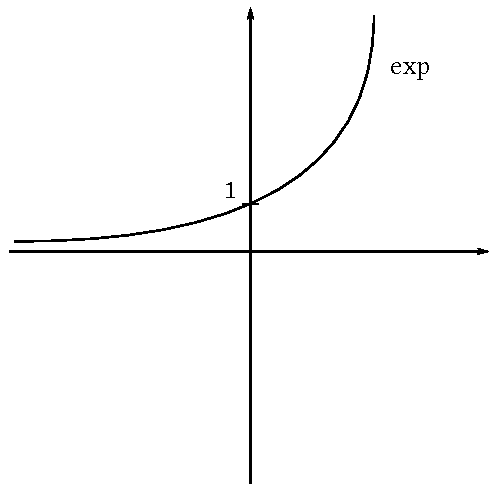
\includegraphics{img/exp-graph.pdf}
    \caption{Graph of the exponential function}
  \end{center}
\end{figure}

Let $n \in \mathbb N$
\[ \lim_{x\to+\infty} \frac{e^x}{x^n} = \infty \]
\[ \lim_{x\to-\infty} e^x \cdot x^n = 0 \]

\section{The natural logarithm}
%
\[ \exp: \mathbb R \to (0,\infty) \]
is injective, because $x_1 < x_2 \implies e^{x_1} < e^{x_2}$

\begin{lemma}
  $\exp: \mathbb R \to (0,\infty)$
  is surjective.
\end{lemma}
\begin{proof}
  We need to show that the equation $e^x = y$ has some solution for every $y > 0$.
  We will use the Intermediate Value Theorem, we discussed in the previous course \enquote{Analysis 1}.

  \begin{description}
    \item[Case 1]
      First of all, let $y \in [1,\infty)$. Then it holds that
      \[ e^0 = 1 \leq y \quad\text{and}\quad e^y = 1 + y + \underbrace{\frac{y^2}{2} + \frac{y^3}{3!} + \frac{y^4}{4!} + \ldots}_{\geq 0} \]
      \[ \geq 1 + y > y \]
      Therefore $e^0 \leq y < e^y$.
      Hence $\exp$ is continuous and the Intermediate Value Theorem applies:
      \[ \exists \xi \in [0,y]: \quad e^\xi = y \]
    \item[Case 2]
      Let $y \in (0,1)$. Then it holds that $w = \frac1{y} > 1$.
      The same as in Case~1 applies:
      \[ \exists \xi \in [0,w]: \quad e^\xi = w = \frac1{y} \]
      \[ \implies e^{-\xi} = \frac{1}{e^\xi} = y \]
  \end{description}

  So it holds that $\exp: \mathbb R \to (0,\infty)$ is bijective.
\end{proof}

\index[English]{Natural logarithm}
\index[German]{\foreignlanguage{ngerman}{Natürlicher Logarithmus}}
\begin{defi}
  We call the inverse function \emph{natural logarithm}\footnote{In non-German literature $\ln(y)$ is almost exclusively written with the more general $\log(y)$.}.
  \[ \exp^{-1}: (0,\infty) \to \mathbb R \]
  \[ \exp^{-1} = \ln(y) = \log(y) \]

  Properties:
  \begin{itemize}
    \item It holds $\forall x \in \mathbb R: \ln(e^x) = x$ and $\forall y \in (0,\infty): e^{\ln(y)} = y$.
    \item $\ln: (0,\infty) \to \mathbb R$ is strictly monotonically increasing
      \begin{proof}
        Let $0 < y_1 < y_2$. Assume $\ln(y_1) \geq \ln(y_2) \xRightarrow{\text{monotonicity}} e^{\ln(y_1)} \geq e^{\ln(y_2)} \implies y_1 \geq y_2$. Contradiction!
      \end{proof}
  \end{itemize}
\end{defi}

\subsection{Functional equations of logarithm}
%
\begin{itemize}
  \item
    For all $x,y > 0$ it holds that
    \[ \ln(x \cdot y) = \ln(x) + \ln(y) \]
  \item Limes:
    \[ \lim_{x \to 1} \frac{\ln(x)}{x - 1} = 1 \]
\end{itemize}
\begin{proof}
  \begin{itemize}
    \item
      \[ x \cdot y = e^{\ln(x \cdot y)} \]
      \[ e^{\ln(x)} \cdot e^{\ln(y)} = e^{\ln(x) + \ln(y)} \]
      Injectivity of $\exp$:
      \[ \ln(x \cdot y) = \ln(x) + \ln(y) \]
    \item
      Let $(x_n)_{n\in\mathbb N}$ with $x_n > 0$ be an arbitrary
      sequence with $\lim_{n\to\infty} x_n = 0$.
      Let $w_n = 1 + x_n$. Then it holds that
      $\lim_{n\to\infty} w_n = 1$ and $y_n = \ln(1 + x_n) = \ln(w_n)$.
      \[ \lim_{n\to\infty} y_n = \ln(1) = 0 \]
      \[ \lim_{n\to\infty} \frac{\ln(w_n)}{w_n - 1} = \lim_{n\to\infty} \frac{y_n}{e^{y_n} - 1} = \frac11 = 1 \]
      where
      \[ e^0 = 1 \implies \ln(1) = 0 \]
      \textbf{Personal notes:}
      I don't understand why this gives $\frac11$, but it is simple to recognize:
      \[ \lim_{x\to1} \frac{\ln{x}}{x-1} = \lim_{x\to0} \frac{\ln(x+1)}{x} = \lim_{x\to0} \frac{\ln(x+1) - \ln(1)}{x} = \left.\ln(t)'\right|_{t=1} = 1 \]
  \end{itemize}
\end{proof}

\begin{theorem}[Logarithmic growth]
  $\forall n \in \mathbb N_+$ it holds that $\lim_{x\to\infty} \frac{\ln(x)}{\sqrt[n]{x}} = 0$
\end{theorem}
\begin{proof}
  Let $x \in (0,\infty)$ with $x = e^{n\cdot\xi}$. That is,
  \[ \xi = \frac{\ln(x)}{n} \]
  \[ x \to \infty \Leftrightarrow \xi \to \infty \]
  \[
    \lim_{x\to\infty} \frac{\ln(x)}{\sqrt[n]{x}}
    = \lim_{\xi\to\infty} \frac{n \cdot \xi}{\sqrt[n]{e^{n \cdot \xi}}}
    = \lim_{\xi\to\infty} \frac{n \cdot \xi}{e^\xi} = 0
  \]
  because $n \cdot \xi < \xi^2$ for $\xi > n$ and $\lim_{\xi\to\infty} \frac{\xi^2}{e^\xi} = 0$.
\end{proof}

\begin{theorem}
  The logarithm function is differentiable in $(0,\infty)$ and it holds that $(\ln(x))' = \frac1x \quad \forall x > 0$.
\end{theorem}
\begin{figure}[!h]
  \begin{center}
    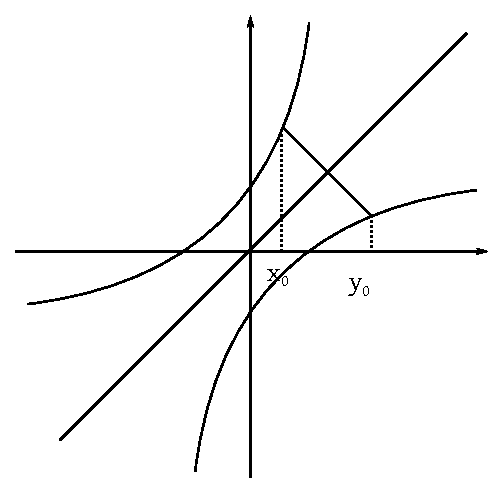
\includegraphics{img/geometric-exp-proof.pdf}
    \caption{A geometric proof of differentiability}
    \label{img:geo-diff}
  \end{center}
\end{figure}
\begin{proof}
  \begin{description}
    \item[First approach]
      Let $x > 0$, $x_n \to x$ with $x_n \neq x$, $x_n > 0$.
      Let $\xi_n = \ln(x_n)$ and $\xi = \ln(x) \implies \xi_n \neq \xi$.
      \[ e^{\xi_n} = x_n \qquad e^\xi = x \qquad \xi_n \to \xi \]
      Then it holds that
      \[ \lim_{n\to\infty} \frac{\ln(x_n) - \ln(x)}{x_n - x} = \lim_{n\to\infty} \frac{\xi_n - \xi}{e^{\xi_n} - e^\xi} \]
      \[
        = \lim_{n\to\infty} \frac{1}{\frac{e^{\xi_n} - e^\xi}{\xi_n - \xi}}
        = \frac{1}{\underbrace{\lim_{n\to\infty} \frac{e^{\xi_n} - e^\xi}{\xi_n - \xi}}_{(e^\xi)' = e^\xi}}
        = \frac1{e^\xi} = \frac1x
      \]
    \item[Second approach using chain rule]
      Compare with Figure~\ref{img:geo-diff}.
      \[ (f^{-1})'(y_0) = \frac{1}{f'(f^{-1}(y_0))} \]
      \[ f(f^{-1}(y)) = y \implies f(f^{-1}) f(f^{-1}(y)) = y = f'(f^{-1}(y)) \cdot (f^{-1})'(y) = 1 \]
      \[ \implies (f^{-1})'(y) = \frac{1}{f'(f^{-1}(y))} \text{ for } f(x) = \exp(x) \]
      \[ \implies (\ln)'(y) = \frac{1}{\exp(\ln(y))} = \frac{1}{y} \]

      \[ f(f^{-1}(y)) = y \]
      \[ f'(f^{-1}(y)) \cdot (f^{-1}) \]
      \[ = (f^{-1})'(y) = \frac{1}{f'(f^{-1}(y))} \]
      again for $f(x) = \exp(x)$.
    \item[Third approach]
      Let $x > 0$.
      \[ 0 = \ln(1) = \ln\left(x \cdot \frac1x\right) = \ln(x) + \ln\left(\frac1x\right) \]
      \[ \implies \ln\left(\frac1x\right) = -\ln(x) \]

      Let $x,y > 0$. Then it holds that
      \[ \ln{\frac{x}{y}} = \ln(x) - \ln(y) \]
      because $\ln\frac{x}{y} = \ln(x \cdot \frac1y) = \ln(x) - \ln(y)$.
  \end{description}
\end{proof}

\subsection{Extension of the functional equation of logarithm}
%
Let $x > 0$.
\[ 0 = \ln(1) = \ln\left(x \cdot \frac1x\right) = \ln(x) + \ln\left(\frac1{x}\right) \]
\[ \implies \ln\frac{1}{x} = -\ln(x) \]
Let $x,y > 0$. Then it holds that
\[ \ln(\frac{x}{y}) = \ln(x) - \ln(y) \]
because $\ln\frac{x}{y} = \ln\left(x \cdot \frac{1}{y}\right) = \ln(x) - \ln(y)$.

\subsubsection{A different proof for the derivative of logarithm}
%
\begin{proof}
  \[
    [\ln(x)]'
    = \lim_{h\to0} \frac{\ln(x + h) - \ln(x)}{h}
    = \lim_{h\to0} \frac{\ln\left(\frac{x+h}{x}\right)}{h}
    = \lim_{h\to0} \frac{\ln\left(1 + \frac{h}{x}\right)}{x \cdot \frac hx}
  \] \[
    = \frac1x \cdot \lim_{h\to0} \frac{\ln\left(1 + \frac{h}{x}\right)}{\frac{h}{x}}
    \text{ where } \frac hx \to 0
  \]
  $1 + \frac{h}{x} = w$ then it holds that $h \to 0 \implies w \to 1$.
  \[ \frac{h}{x} = w - 1 \]
  \[ \lim_{h\to0} \frac{\ln\left(1 + \frac{h}{x}\right)} = \lim_{h\to0} \frac{\ln(w)}{w - 1} = 1 \]
\end{proof}

\begin{rem}
  The exponential function can be defined from $\mathbb C$ to $\mathbb C$.
  \[ \exp: \mathbb C \to \mathbb C \]
  It is not possible to define the logarithm \emph{continuously} in entire $\mathbb C$
  (or $\mathbb C \setminus \set{0}$). We can only define a continuous inverse function
  of $\exp$ in $\mathbb C \setminus \set{x \in \mathbb R: x \leq 0}$
\end{rem}

\begin{figure}[!h]
  \begin{center}
    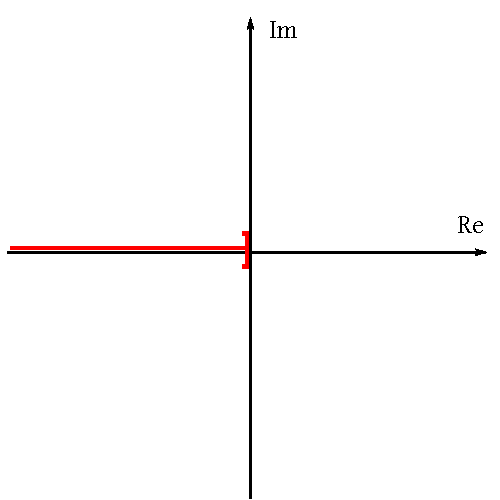
\includegraphics{img/continuous-exp-in-C.pdf}
    \caption{Continuous exponential function in $\mathbb C$}
  \end{center}
\end{figure}

\meta{lecture}{3rd of March 2016}{Wolfgang Ring}

\subsection{Further remarks on differential calculus}

\begin{theorem}
  Let $f: I \to \mathbb R$ be strictly monotonically increasing (or s. m. decreasing)
  where $I$ is an interval. Then $f^{-1}: f(I) \to \mathbb R$ is defined and the inverse function.

  Let $f$ in $x_0 \in I$ be differentiable and $f'(x_0) \neq 0$. Then $f^{-1}$ is in $y_0 = f(x_0)$
  differentiable and it holds that
  \[ (f^{-1})'(y_0) = \frac{1}{f'(x_0)} = \frac{1}{f'(f^{-1}(y_0))} \]
\end{theorem}

\begin{proof}
  Let $y_n \to y_0$ and $y_n \in f(I)$; $y_0 = f(x_0)$; $y_0 \in f(I)$; $y_n = f(x_n)$.
  $y_n \neq y_0 \implies x_n \neq x_0$.
  \[ \lim_{n\to\infty} \frac{f^{-1}(y_n) - f^{-1}(y_0)}{y_n - y_0} \]
  \[
    = \lim_{n\to\infty} \frac{x_n - x_0}{f(x_n) - f(x_0)}
    = \frac{1}{\lim_{n\to\infty} \underbrace{\frac{f(x_n) - f(x_0)}{x_n - x_0}}}_{\text{ex} = f'(x_0)} = \frac{1}{f'(x_0)}
  \]
\end{proof}

\begin{lemma}
  \label{lemma:const-diff}
  Let $f: I \to \mathbb R$ where $I$ is some interval. Then it holds that
  \[ f = \text{ const} \Leftrightarrow f \text{ is differentiable in $I$ and } f'(x) = 0 \forall x \in I \]
\end{lemma}
\begin{proof}
  \begin{description}
    \item[$\Rightarrow$]
      Immediate.
    \item[$\Leftarrow$]
      Let $f$ be differentiable and $f' \equiv 0$.
      Assume $f$ is not constant. Then there exist $x_1, x_2 \in I$, $x_1 \neq x_2$
      and $f(x_1) \neq f(x_2)$. Without loss of generality, $x_1 < x_2$.
      The Intermediate Value Theorem states that
      \[ \exists \xi \in (x_1, x_2) \subseteq I: f'(\xi) = \frac{f(x_2) - f(x_1)}{x_2 - x_1} \neq 0 \]
      This is a contradiction to the assumption that $f' \equiv 0$.
  \end{description}
\end{proof}

\index[English]{Primitive}
\index[German]{\foreignlanguage{ngerman}{Stammfunktion}}
\begin{defi}
  Let $I$ be an interval, $f: I \to \mathbb R$.
  A function $F: I \to \mathbb R$ is called \emph{primitive} or \emph{antiderivative} of $f$
  if $F$ is differentiable and
  \[ \forall x \in I: F'(x) = f(x) \]
\end{defi}
\begin{lemma}
  Let $f: I \to \mathbb R$. Let $F_1$ and $F_2$ be two primitive functions of $f$.
  Then it holds that $F_1 - F_2 = \text{const}$.
\end{lemma}
\begin{proof}
  $F_1$, $F_2$ are differentiable.
  \[ (F_1 - F_2)'(x) = F_1'(x) - F_2'(x) = f(x) - f(x) = 0 \]
  \[ \xRightarrow{\text{Lemma~\ref{lemma:const-diff}}} F_1 - F_2 = \text{ const} \]
\end{proof}

\begin{theorem}
  Let $I$ be an interval.
  Let $(f_n)_{n\in\mathbb N}$ be a sequence of differentiable functions in $I$.
  \[ f_n: I \to \mathbb R \text{ differentiable} \]
  Furthermore let $f: I \to \mathbb R$.
  It holds that,
  \begin{enumerate}
    \item
      $\forall x \in I$ let $f(x) = \lim_{n\to\infty} f_n(x)$
      ($f_n \to f$ pointwise)
    \item
      for every $x \in I$ let $(f'_n(x))_{n\in\mathbb N}$ be convergent
      (hence $\varphi(x) = \lim_{n\to\infty} f_n'(x)$ exists for every $x$)
    \item
      $\forall \varepsilon > 0 \exists N \in \mathbb N$ such that
      \[ n \geq N \Rightarrow \abs{(f_n - f)(u) - (f_n - f)(v)} \leq \varepsilon \abs{u - v} \forall u,v \in I \]
      Then $f$ is differentiable in $I$ and it holds that $f'(x) = \varphi(x) = \lim_{n\to\infty} f'_n(x)$.
      \[ f'(x) = [\lim_{n\to\infty} f]'(x) \]
  \end{enumerate}
\end{theorem}
\begin{proof}
  Let $x_0 \in I$ and $x \in I$. Let $\varepsilon > 0$ arbitrary.
  \[ \abs{\frac{f(x) - f(x_0)}{x - x_0} - \varphi(x_0)} \]
  \[ = \abs{\frac{f(x) - f(x_0)}{x - x_0} - \lim_{n\to\infty} f_N'(x_0)} \]
  \[ = \abs{\frac{f(x) - f(x_0)}{x - x_0} - f'_N(x_0)} + \abs{f'_N(x_0) - \lim_{n\to\infty} f'_n(x_0)} \forall N \in \mathbb N \]
  \[
    \leq \abs{\frac{f(x) - f(x_0)}{x - x_0} - \frac{f_N(x) - f_N(x_0)}{x - x_0}}
  \] \[
    + \abs{\frac{f_N(x) - f_N(x_0)}{x - x_0} - f'_N(x_0)}
    + \abs{f'_N(x_0) - \varphi(x_0)}
  \]

  \begin{description}
    \item[1st term]
      \[
        \abs{\frac{(f(x) - f_N(x)) - (f(x_0) - f_N(x_0))}{x - x_0}}
        = \abs{\frac{(f - f_N)(x) - (f - f_N)(x_0)}{x - x_0}}
      \] \[
        \leq \frac\varepsilon3 \frac{\abs{x - x_0}}{\abs{x - x_0}}
        \stackrel{\text{condition 3}}{=} \frac{\varepsilon}{3}
      \]
      for sufficiently large $N$.
    \item[3rd term]
      $\abs{f'_N(x_0) - \varphi(x)} < \frac{\varepsilon}{3}$ for sufficiently large $N$.
  \end{description}

  Now let $N$ be fixed (with a value such that the first and third term is less than $\frac\varepsilon3$).

  \begin{description}
    \item[2nd term]
      \[ \abs{\frac{f_N(x) - f_N(x_0)}{x - x_0}} - f'_N(x_0) \]
  \end{description}

  Differentiability of $f_N$:
  Therefore for $\abs{x - x_0} < \delta$.
  \[
    \abs{\frac{f(x) - f(x_0)}{x - x_0} - \varphi(x_0)}
    < \frac\varepsilon3 + \frac\varepsilon3 + \frac\varepsilon3
    = \varepsilon
  \]
  $f$ is differentiable in $x_0$ and $f'(x_0) = \varphi(x_0)$.
\end{proof}

\begin{theorem}
  Let $f_n: I \to \mathbb R$ and $f: I \to \mathbb R$ ($n \in \mathbb N$)
  and $f_n$ is differentiable in $I$.

  Assumption:
  \begin{enumerate}
    \item $f_n \to f$ converges pointwise in $I$
      (like the first statement in the previous Theorem)
    \item There exists $g: I \to \mathbb R$ such that
      $f'_n \to g$ is uniformly continuous in $I$, hence
      \[
        \forall \varepsilon > 0 \exists N \in \mathbb N: n \geq N, x \in I
        \implies \abs{f_n'(x) - g(x)} < \varepsilon
      \]
  \end{enumerate}
  Then $f$ is differentiable in $I$ and it holds that
  \[ f'(x_0) = g(x_0) \quad \forall x_0 \in I \]
\end{theorem}

\meta{lecture}{4th of March 2016}{Wolfgang Ring}

\begin{theorem}[Reminder of theorem]
  \label{thm:diff-conv}
  Let $(f_n)_{n\in\mathbb N}$ be a sequence of functions in $I$ and
  let $f_n$ be differentiable $\forall n \in \mathbb N$. Furthermore,
  \begin{itemize}
    \item $f_n \to f$ pointwise
    \item $f'_n(x) \to \varphi(x)$ for every $x$
    \item $\forall \varepsilon > 0 \forall u,v \in I \exists N: n \geq N
      \implies \abs{(f_n - f)(u) - (f_n - f)(v)} < \varepsilon \abs{u - v}$
  \end{itemize}
  Then it holds that $f$ is differentiable and $f'(x) = \varphi(x) \forall x \in I$.
\end{theorem}

Conclusion:
\begin{theorem}
  \label{thm:concl}
  Let $f_n$ and $f$ be differentiable as in Theorem~\ref{thm:diff-conv}:
  $f_n: I \to \mathbb R$ and $f: I \to \mathbb R$ and it holds that
  \begin{itemize}
    \item $f_n \to f$ pointwise in $I$ for $n \to \infty$
    \item $\exists g: I  \to \mathbb R$ such that $f'_n \to g$ is \emph{uniform} in $I$,
      hence $\forall \varepsilon > 0 \exists N \in \mathbb N:
      n \geq N \land x \in I \implies \abs{f'_n(x) - g(x)} < \varepsilon$
  \end{itemize}
  Then $f$ is differentiable in $I$ and $f'(x) = g(x) \forall x \in I$.
\end{theorem}
\begin{proof}
  We check whether the two conditions lead to the conditions of Theorem~\ref{thm:diff-conv}.

  We look at the conditions of Theorem~\ref{thm:diff-conv}:
  \begin{itemize}
    \item[2.] Uniform convergences of $f'_n \to g$ implies pointwise convergence
      \[ \forall x \in I: f'_n(x) \to g(x) \]
    \item[3.] From uniform convergence of $f'_n \to g$ it follows that
      Let $\varepsilon > 0$ be arbitrary and $N$ is sufficiently large enough, such that
      $\forall n \geq N$ and $\forall x \in I$:
      \[ \abs{f_n'(x) - g(x)} < \frac\varepsilon2 \]
      Choose $n,m \geq N$ and $x \in I$ arbitrary. Then it holds that
      \[ \abs{f'_n(x) - f'_m(x)} = \abs{f'_n(x) - g(x) + g(x) - f'_m(x)} \]
      \[ \leq \abs{f'_n(x) - g(x)} + \abs{g(x) - f'_m(x)} < \frac\varepsilon2 + \frac\varepsilon2 = \varepsilon \]
      So $(f_n)_{n\in\mathbb N}$ is a uniform Cauchy sequence.

      Let $\varepsilon > 0$ be arbitrary and $N$ such that $n,m \geq N$ and $x \in I$:
      \[ \abs{f'_n(x) - f'_m(x)} < \varepsilon \]

      Consider the third condition of Theorem~\ref{thm:diff-conv}. Let $u,v \in I$
      \[ \abs{(f - f_n)(u) - (f - f_n)(v)} = \lim_{m\to\infty} \abs{(f_m - f_n)(u) - (f_m - f_n)(v)} \]
      where $(f_m - f_n)$ and $(f_m - f_n)$ is differentiable. Then according to the
      mean value theorem of differential calculus (dt. Mittelwertsatz der Differentialrechnung)
      \begin{align*}
        &= \lim_{m\to\infty} \abs{(f_m - f_n)'(\xi_{m,n}) \cdot (u - v)} \\
        &= \lim_{m\to\infty} \abs{f'_m(\xi_{m,n}) - f'_n(\xi_{m,n})} \cdot \abs{u - v}
      \end{align*}
      For $m \geq N$:
      \[ \leq \varepsilon \cdot \abs{u - v} \]
      So the third condition of Theorem~\ref{thm:diff-conv} is satisfied.
  \end{itemize}
\end{proof}

\begin{figure}[!h]
  \begin{center}
    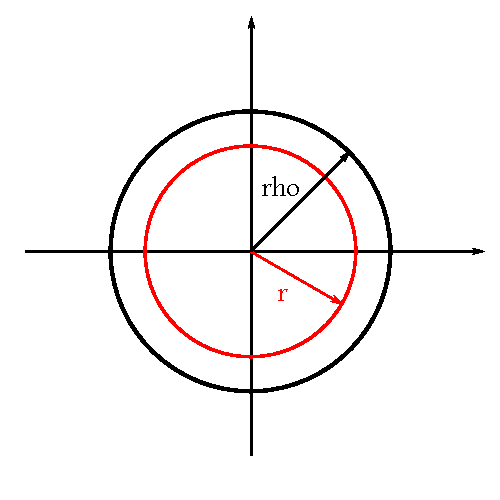
\includegraphics{img/convergence_radius.pdf}
    \caption{Convergence radius}
    \label{fig:convr}
  \end{center}
\end{figure}


\begin{rem}[An application of Theorem~\ref{thm:concl}]
  Let $P(z) = \sum_{k=0}^\infty a_k z^k$ be a power series with convergence radius $\rho(P)$ with
  \[ \rho(P) = \frac1L \qquad L = \limsup_{n\to\infty} \sqrt[n]{\abs{a_n}} \]
  \[ P_n(z) = \sum_{k=0}^n a_k z^k \qquad \text{\dots $n$-th partial sum} \]
  Let $r < \rho(P)$. Then it holds that $P_n(z) \to P(z)$ uniform in $\overline{B(0,r)}$~\footnote{Where overline means \enquote{closed}}.
  \[ P_n(x) \to P(x) \forall x \in [-r, r] \]

  Compare with Figure~\ref{fig:convr}.

  \[ P'_n(x) = \sum_{k=0}^n a_k k \cdot x^{k-1} = \sum_{j=0}^{n-1} a_{j+1} (j + 1) x^j \]
  is the $n-1$-th partial sum.
  \[ Q(z) = \sum_{j=0}^\infty a_{j+1} (j + 1) z^j \]
  Convergence radius of $Q$?
  \[ \tilde{L} = \limsup_{j\to\infty} \sqrt[j]{a_{j+1}} \cdot \sqrt[j]{j + 1} = \limsup_{j \to \infty} \abs{a_{j+1}}^{\frac{j+1}{j} \cdot \frac{1}{j+1}} \cdot (j+1)^{\frac{j+1}{j} \cdot \frac{1}{j+1}} \]
  \[
    = \limsup_{j\to\infty} \underbrace{\left(\abs{a_{j+1}}^{\overbrace{\frac{1}{j+1}}^{\to 1}}\right)^{\frac{j+1}{j}}}_{L^1 = L}
    \cdot \underbrace{\lim_{j\to\infty} \left[(j+1)^{\frac{1}{j+1}}\right]^{\frac{j+1}{j}}}_{1^1}
    = L
  \]
  In conclusion we have $\tilde L = L$ and $\rho(Q) = \frac1{L} = \rho(P)$.
  So $P'_n(z) = \sum_{k=1}^n k \cdot a_k z^{k-1}$ uniformly convergent in $\overline{B(0,r)}$ for $r<\rho$
  and therefore also uniformly convergent  in $[-r,r]$.

  From Theorem~\ref{thm:concl} it follows that $P(x)$ is differentiable
  in $[-r,r]$ and $P'(x) = \sum_{k=1}^\infty k \cdot a_k \cdot x^{k-1}$.

  Let $\abs{x} < \rho(P)$. Let $r = \frac12 (\abs{x} + \rho(P))$, then it holds that
  $x \in [-r, r]$ and $P$ is differentiable in point $x$ with
  \[ P'(x) = \sum_{k=1}^\infty k \cdot a_k \cdot x^{k-1} \]
\end{rem}

\begin{lemma}
  Let $P(z) = \sum_{k=0}^\infty a_k z^k$ be a power series with convergence radius $\rho(P) > 0$.
  Let $x \in (-\rho(P), \rho(P))$. Then $P$ is differentiable in $x$ and it holds that
  \[ P'(x) = \sum_{k=1}^\infty k \cdot a_k \cdot x^{k-1} \]

  Furthermore the power series $\sum_{k=1}^\infty k \cdot a_k \cdot x^{k-1}$ is uniformly convergent
  in every interval $[-r, r]$ with $0 < r < \rho(P)$.
\end{lemma}

\subsection{About logarithm functions}
%
We consider the power series
\[ g(z) = \sum_{k=1}^\infty \frac{z^k}{k} \]
\[ \rho(g) = \frac1L \text{ with } L = \limsup_{k\to\infty} \sqrt[k]{\frac1k} = \frac{1}{\lim_{k\to\infty} \sqrt[k]{k}} = 1 \]
So it holds that $\rho(g) = 1$.

Apply the previous theorem, followingly $g$ is differentiable in $(-1,1)$ and it holds that
\[ g'(x) = \sum_{k=1}^\infty \frac{k}{k} x^{k-1} = \sum_{j=0}^\infty x^j = \frac1{1 - x} \]

Remark:
\[ \left[-\ln(1 - x)\right]' = -\frac{1}{1 - x} \cdot (-1) = \frac1{1 - x} \]
\[ \implies \sum_{k=1}^\infty \frac{x^k}{k} + \ln(1 - x) = \text{ constant} \]
Let $x = 0$ (we determine the constant for this $x=0$):
\[ 0 + 0 = 0 = \text{ constant} \]
\[ \implies \ln(1 - x) = -\sum_{k=1}^\infty \frac{x^k}{k} \qquad \text{ for } \abs{x} < 1 \]

Let $x \in (-1,1) \Rightarrow -x \in (-1,1)$.
\[ \implies \ln(1 - (-x)) = \ln(1 + x) = -\sum_{k=1}^\infty \frac{(-x)^k}{k} \]
\[ = \sum_{k=1}^\infty \frac{(-1)^{k-1} \cdot x^k}{k} = x - \frac{x^2}{2} + \frac{x^3}{3} - \frac{x^4}{4} + \ldots \]

\index[English]{Logarithmic series}
\index[German]{\foreignlanguage{ngerman}{Logarithmische Reihe}}
Therefore: We introduce \emph{logarithmic series}:
\[ \ln(1 - x) = -\sum_{k=1}^\infty \frac{x^k}{k} \]
\[ \ln(1 + x) = \sum_{k=1}^\infty \frac{(-1)^{k-1} x^k}{k} \]
\[
  \ln\left(\frac{1 + x}{1 - x}\right)
  = \ln(1 + x) - \ln(1 - x)
  = 2 \sum_{l=1}^\infty \frac{x^{2l - 1}}{2l - 1}
  \quad \text{ for } x \in (-1,1)
\]

\begin{figure}[!h]
  \begin{center}
    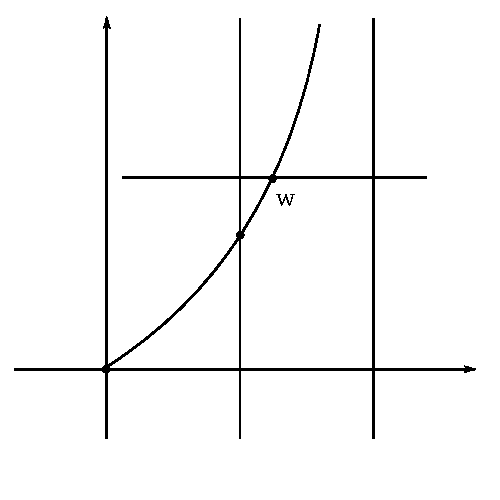
\includegraphics{img/1x_1-x.pdf}
    \caption{Plot of $\frac{1+x}{1-x}$}
    \label{img:1x-1x}
  \end{center}
\end{figure}

\[ f(x) = \frac{1 + x}{1 - x} \]
Compare with Figure~\ref{img:1x-1x}.
\[ f'(x) = \frac{1 - (-1)}{(1 - x)^2} = \frac{2}{(1 - x)^2} > 0 \quad \text{ in } (-1, 1) \]
Solve $\frac{1 + x}{1 - x} = w$ for $x$.

\[ \implies 1 + x  = w - wx \]
\[ x (1 + w) = w - 1 \]
\[ x = \frac{w - 1}{w + 1} \]

\[ \ln(w) = 2 \sum_{l=1}^\infty \frac{x^{2l-1}}{2l - 1} \]

\section{Trigonometic functions}

We define trigonometic functions using the exponential function in $\mathbb C$.

Let $t \in \mathbb R$.
\[ e^{it} = \sum_{k=0}^\infty \frac{(it)^k}{k!} = \lim_{n\to\infty} \left(\underbrace{1}_{\mathbb R} + \underbrace{\frac{it}{n}}_{i \mathbb R}\right)^n \]
\[
  e^{-it}
    = \lim_{n\to\infty} \left(1 - \frac{it}{n}\right)^n
    = \lim_{n\to\infty} \left[\overline{\left(1 + \frac{it}{n}\right)}\right]^n
\] \[
  = \lim_{n\to\infty} \overline{\left(1 + \frac{it}{n}\right)^n}
  = \overline{\lim_{n\to\infty} \left(1 + \frac{it}{n}\right)^n}
  = e^{it}
\] \[
  \abs{e^{it}}^2 = e^{it} \cdot \overline{e^{it}} = e^{it} \cdot e^{-it}
\] \[
  e^{it - it} = e^0 = 1
\]
So it holds that $\forall t \in \mathbb R$:
\[ \abs{e^{it}} = 1 \]
So $e^{it}$ lies inside the complex unit circle. Compare with Figure~\ref{img:unitc}.

\begin{figure}[!h]
  \begin{center}
    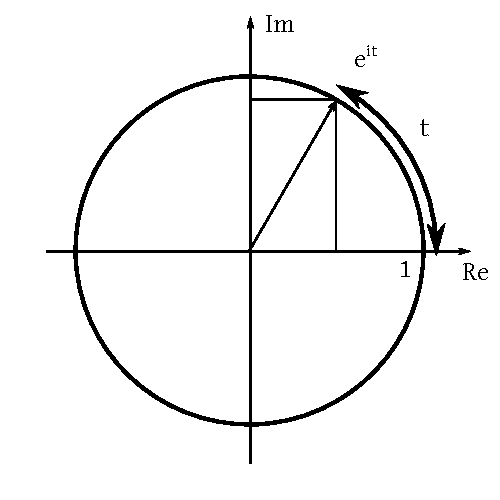
\includegraphics{img/unitcircle_in_C.pdf}
    \caption{Unit circle in $C$ with $t$}
    \label{img:unitc}
  \end{center}
\end{figure}

\index[English]{Sine function}
\index[German]{\foreignlanguage{ngerman}{Sinusfunktion}}
\index[English]{Cosine function}
\index[German]{\foreignlanguage{ngerman}{Cosinusfunktion}}
We define the cosine function $\cos: \mathbb R \to \mathbb R$ as
\[ \cos(t) = \Re(e^{it}) \]
and the sine function $\sin: \mathbb R \to \mathbb R$ as
\[ \sin(t) = \Im(e^{it}) \]

The following relations hold:
\begin{enumerate}
  \item $e^{it} = \cos(t) + i \cdot \sin(t)$ (Euler's identity)
  \item $\abs{e^{it}}^2 = 1 = (\cos{t})^2 + (\sin{t})^2$
  \item \[ \Re(z) = \frac12 (z + \overline{z}) \]
    \[ \Rightarrow \cos(t) = \Re(e^{it}) = \frac12 \left(e^{it} + e^{-it}\right) \]
    \[ \Im(z) = \frac1{2i} [z - \overline{z}] \]
    \[ \sin(t) = \Im(e^{it}) = \frac{1}{2i} \left[e^{it} - e^{-it}\right] \]
  \item
    \[ e^{-it} = \overline{e^{it}} = \cos{t} - i \cdot \sin{t} \]
\end{enumerate}

We use property 3 to extend the domain of sine and cosine:
\begin{defi}
  Let $z \in \mathbb C$. We define $\sin: \mathbb C \to \mathbb C$
  and $\cos: \mathbb C \to \mathbb C$ by
  \[ \cos(z) = \frac12 \left[e^{iz} + e^{-iz}\right] \]
  \[ \sin(z) = \frac1{2i} \left[e^{iz} - e^{-iz}\right] \]
\end{defi}

\meta{lecture}{8th of March 2016}{Wolfgang Ring}

\begin{figure}
  \begin{center}
    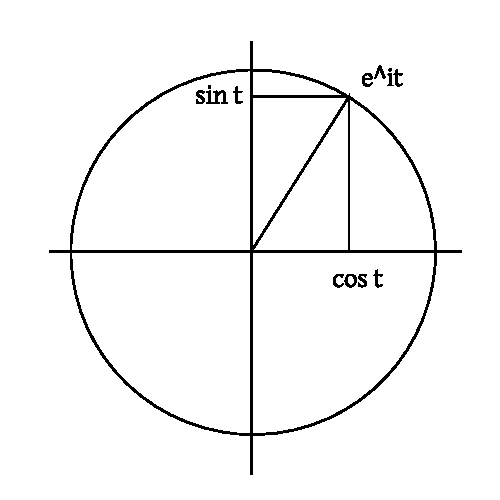
\includegraphics{img/complex_unit.pdf}
    \caption{The trigonometric values $\sin{t}$ and $\cos{t}$ in the unit circle}
    \label{img:cossin}
  \end{center}
\end{figure}
%
Compare with Figure~\ref{img:cossin}.

\begin{align*}
  t \in \mathbb R:
    \cos{t} = \Re(e^{it}) = \frac12 (e^{it} + e^{it}) \\
    \sin{t} = \Im(e^{it}) = \frac{1}{2i} (e^{it} - e^{-it})
\end{align*}

\begin{align*}
  z \in \mathbb C:
    \cos{z} &= \frac12 (e^{iz} + e^{-iz}) \\
    \sin{z} &= \frac{1}{2i} (e^{iz} - e^{-iz})
\end{align*}

Properties:
\begin{align*}
  \cos{-z} &= \frac12 (e^{i(-z)} + e^{-i}(-z)) = \cos{z} \\
  \intertext{$\cos{z}$ is even}
  \sin{-z} &= \frac1{2i} (e^{-iz} - e^{iz}) = -\sin{z}
  \intertext{$\sin{z}$ is odd}
\end{align*}

The cosine function in the complex space is even.

\subsection{Series representation of trigonometric functions}

\begin{lemma}[Addition of series of absolute convergence]
  Let $(a_n)_{n\in\mathbb N}$, $(b_n)_{n\in\mathbb N}$ be complex sequences
  and the series $\sum_{n=0}^\infty a_n$ and $\sum_{n=0}^\infty b_n$ are absolute
  convergent with series value $\sum_{n=0}^\infty a_n = a$ and $\sum_{n=0}^\infty b_n = s'$.

  Then $\sum_{n=0}^\infty (a_n + b_n)$ is absolute convergent with sum $s + s'$.
\end{lemma}
\begin{proof}[Proof for series sum:]
  Consider absolute convergence.
  Show that $\sum_{k=0}^n = \abs{a_k + b_k} = t_n$ and $(t_n)_{n\in\mathbb N}$ is bounded.

  Follows immediately, because
  \[ \sum_{k=0}^n \abs{a_kk + b_k} \leq \underbrace{\sum_{k=0}^n \abs{a_k}}_{\text{bounded}} + \underbrace{\sum_{k=0}^n \abs{b_k}}_{\text{bounded}} \]
\end{proof}

\begin{ex}[Application]
  Let $P(z) \coloneqq \sum_{k=0}^\infty a_k z^k$ and $Q(z) \coloneqq \sum_{k=0}^\infty b_k z^k$ be power series.
  Both are convergent in $B(0, \delta)$. Then also $\sum_{k=0}^\infty (a_k + b_k) z^k$ is convergent in $B(0,\delta)$
  and it holds that $\sum_{k=0}^\infty (a_k + b_k) z^k = P(z) + Q(z)$.
\end{ex}

\subsection{Application to trigonometric functions}
%
\[ e^{iz} = \sum_{k=0}^\infty \frac{(iz)^k}{k!} = \sum_{k=0}^\infty i^k \cdot \frac{z^k}{k!} \]
\[ i^0 = 1 \qquad i^1 = i \qquad i^2 = -1 \qquad i^3 = -i \qquad i^4 = 1 = i^0 \qquad i^5 = i \qquad \ldots \]
\[ \Rightarrow = 1 + i \frac{z}{1!} - \frac{z^2}{2!} - i \frac{z^3}{3!} + \frac{z^4}{4!} + i \frac{z^5}{5!} - \frac{z^6}{6!} \]

\[ e^{-iz} = \sum_{k=0}^\infty \frac{(-iz)^k}{k!} = \sum_{k=0}^\infty (-i)^k \frac{z^k}{k!} \]
\[ (-i)^0 = 1 \qquad (-i)^1 = -i \qquad (-i)^2 = -1 \qquad (-i)^3 = i \qquad (-i^4) = 1 \qquad \ldots \]
\[ \Rightarrow = 1 - i \frac{z}{1!} - 1\frac{z^2}{2!} + i \frac{z^3}{3!} + \frac{z^4}{4!} - i \frac{z^5}{5!} - \frac{z^6}{6!} + \ldots \]

\[ \frac12 (e^{iz} + e^{-iz}) = 1 - \frac{z^2}{2!} + \frac{z^4}{4!} - \frac{z^6}{6!} + \frac{z^8}{8!} - \frac{z^{10}}{10!} + \ldots \]

Followingly,
\begin{align*}
  \cos{z} &= 1 - \frac{z^2}{2!} + \frac{z^4}{4!} - \frac{z^6}{6!} + \frac{z^8}{8!} - \ldots \\
          &= \sum_{l=0}^\infty (-1)^l \frac{z^{2l}}{(2l)!} \text{ convergent in } \mathbb C \\
  \sin{z} &= \frac1{2i}(e^{iz} - e^{-iz}) = z - \frac{z^3}{3!} + \frac{z^5}{5!} - \frac{z^7}{7!} + \frac{z^9}{9!} + \ldots \\
          &= \sum_{l=0}^\infty (-1)^l \frac{z^{2l + 1}}{(2l+1)!}
\end{align*}

\subsection{Functional equations of trigonometric functions}
%
\begin{theorem}[Addition and substraction theorems]
  We derive them directly:

  Let $z,w \in \mathbb C$.
  \begin{align*}
    e^{z+w} &= e^z \cdot e^w = (\cos{z} + i \cdot \sin{z}) (\cos{w} + i \cdot \sin{w}) \\
    \intertext{but also}
            &= (\cos(z + w) + i \sin(z + w)) \\
            &\Rightarrow = (\cos{z} \cdot \cos{w} - \sin{z} \cdot \sin{w}) + i (\cos{z} \cdot \sin{w} + \sin{z} \cdot \cos{w})
  \end{align*}

  Analogously,
  \begin{align*}
    e^{-(z+w)} &= e^{-z} \cdot e^{-w} = (\cos(-z) + i \cdot \sin(-z)) (\cos(-w) + i \cdot \sin(-w)) \\
               &= \cos{z} \cdot \cos{w} - \sin{z} \sin{w} + i \left(-\cos{z} \sin{w} - \cos{w} \sin{z}\right) \\
    \intertext{but also}
            &= (-\cos(z + w) + i \sin(-(z + w))) \\
            &\Rightarrow = \cos{(z + w)} - i \sin(z + w)
  \end{align*}

  \begin{align*}
    \intertext{Addition (cosine):}
    2 \cos(z+w) &= 2 (\cos{z} \cdot \cos{w} - \sin{z} \sin{w}) \\
    \Rightarrow \cos(z + w) &= \cos{z} \cos{w} - \sin{z} \sin{w}
    \intertext{Addition (sine):}
    \Rightarrow \sin(z + w) &= \cos{z} \sin{w} + \sin{z} \cos{w} \forall z,w \in \mathbb C
  \end{align*}

  Substraction (hence $w \leftrightarrow -w$):
  \begin{align*}
    \cos(z - w) &= \cos{z} \cdot \underbrace{\cos{w}}_{=\cos(-w)} + \sin{z} \underbrace{\sin{w}}_{=-\sin(-w)} \\
    \sin(z - w) &= -\cos{z} \cdot \sin(w) + \sin(z) \cos(w)
  \end{align*}
\end{theorem}

\begin{cor}
  \[ z = \frac12 (z + w) + \frac12 (z - w) \]
  \[ \Rightarrow \cos{z} = \cos{\frac{z + w}{2}} \cos{\frac{z - w}{2}} - \sin{\frac{z + w}{2}} \sin{\frac{z - w}{2}} \]
  \[ w = \frac12 (w + z) + \frac12 (w - z) = \frac12 (z + w) - \frac12 (z - w) \]
  \[ \cos{w} = \cos{\frac{z + w}{2}} \cdot \cos{\frac{z - w}{2}} + \sin{\frac{z + w}{2}} \cdot \sin{\frac{z - w}{2}} \]
  \[ \cos{z} - \cos{w} = -2 \sin{\frac{z + w}{2}} \sin{\frac{z - w}{2}} \]
  Analogously,
  \[ \sin{z} - \sin{w} = 2 \cos{\frac{z + w}{2}} \cdot \cos{\frac{z - w}{2}} \]
\end{cor}

We consider
\begin{align*}
  \lim_{\substack{z \to 0 \\ z \neq 0}} \frac{\sin{z}}{z}
    &= \lim_{z \to 0} \frac{1}{2i} \left(\frac{e^{iz} - e^{-iz}}{z}\right) \\
    &= \lim_{z \to 0} e^{-iz} \left(\frac{e^{2iz} - 1}{2iz}\right) \\
    &= \underbrace{\lim_{z \to 0} e^{-iz}}_{=e^0 = 1} \cdot \underbrace{\lim_{z \to 0} \frac{e^{2iz} - 1}{2iz}}_{\substack{e = 2iz; z \to 0 \Leftrightarrow w = 0 \\ \lim_{w \to 0} \frac{e^w - 1}{w} = 1}}
\end{align*}

So it holds that
\[ \lim_{z\to0} \frac{\sin{z}}{z} = 1 \]

\subsection{Trigonometric functions for real arguments}
%
Subtitled \enquote{definition of $\pi$} and \enquote{periodicity}.

Let $x \in \mathbb R$.
\[ \cos{x} = \overbrace{1}^{=c_0} - \overbrace{\frac{x^2}{2}}^{=c_1} + \overbrace{\frac{x^4}{24}}^{=c_2} - \overbrace{\frac{x^6}{720}}^{=c_3} + \overbrace{\frac{x^8}{40320}}^{=c_4} - \ldots \]
\[ \sin{x} = \underbrace{x}_{=s_0} - \underbrace{\frac{x^3}{6}}_{=s_1} + \underbrace{\frac{x^5}{120}}_{=s_2} - \underbrace{\frac{x^7}{5040}}_{=s_3} + \ldots \]

\[ c_n = \frac{x^{2k}}{(2k)!} \qquad s_k = \frac{x^{2k+1}}{(2k+1)!} \]

For $x \in [0,2]$ and $k \geq 1$ it holds that
\[ \abs{\frac{c_{k+1}}{c_k}} = \abs{\frac{x^2}{(2k + 2)(2k + 1)}} \leq \frac{4}{3 \cdot 4} = \frac13 \]
so $(c_k)_{k\geq1}$ is strictly monotonically decreasing.

Leibniz criterion:
\[ 1 - \frac{x^2}{2} < \cos{x} < 1 - \frac{x^2}{2} + \frac{x^4}{24} \]
for $x \in (0,2]$.

Similarly for $x \in (0,2]$:
\[ \abs{\frac{s_{k+1}}{s_k}} = \abs{\frac{x^2}{(2k + 2)(2k + 3)}} \leq \frac{4}{4 \cdot 5} = \frac15 < 1 \]
So the Leibniz criterion tells us that
\[ x - \frac{x^3}{6} < \sin{x} < x \quad \text{ in } [0, 2] \]
So it holds that
\[ \cos(0) = 1 \]
\[ \cos(2) < 1 - 2 + \frac{16}{24} = -1 + \frac23 = -\frac13 \]
Intermediate value theorem (power series is continuous):
\[ \exists \xi \in (0,2) \text{ with } \cos(\xi) = 0 \]
Let $0 \leq w < z \leq 2$,
\[ 0 < \frac{z-w}{2} \leq \frac{z+w}{2} < \frac{z + z}{2} \leq 2 \]

Let $x \in (0,2]$, then it holds that
\[ \sin(x) > x - \frac{x^3}{6} = \underbrace{x}_{>0} \underbrace{\left(1 - \frac{x^2}{6}\right)}_{>1 - \frac46 = \frac13 > 0} > 0 \]
So it holds that $\sin(x) > 0$ in $(0,2]$.

Functional equation for $\cos{z} - \cos{w}$.
\[ \cos{z} - \cos{w} = \underbrace{-2  \cdot \underbrace{\sin{\underbrace{\frac{z+w}{2}}_{\in (0,2]}} \cdot \sin{\underbrace{\frac{z-w}{2}}_{\in (0,2]}}}_{>0}}_{<0} \]
$\cos{z} < \cos{w}$ for $0 \leq w < z \leq 2$.

So it holds that $\cos$ is a strictly monotonically decreasing functionin $[0,2)$. Hence $\cos$ has only one root because it is continuous in $(0,2]$.

\begin{defi}
  The number $\pi \in \mathbb R$ is defined as $\pi = 2\xi$, where $\xi$ is the uniquely defined root of the cosine in $(0,2]$.
\end{defi}

Some further important function values:
\[ 0 < \frac{\pi}{2} < 2 \text{ and } \cos{\frac\pi2} = 0 \]
because $\cos^2\left(\frac\pi2\right) + \sin^2\left(\frac\pi2\right) = 1$.
\[ \Rightarrow \abs{\sin\frac\pi2} = 1 \]
We know that $\sin{x} > 0$ for $x \in (0,2]$.
\[ \Rightarrow \sin\frac\pi2 = 1 \]

\[ e^{i \frac\pi2} = \cos\frac\pi2 + i \sin\frac\pi2 = i \]
\[ e^{i\pi} = e^{i\frac\pi2 + i\frac\pi2} = \left(e^{i\frac\pi2}\right)^2 = i^2 = -1 \]
\[ e^{i \frac32\pi} = e^{i\pi + \frac{i}2 \pi} = e^{i\pi} \cdot e^{i \frac\pi2} = -1 \cdot i = -i \]

Furthermore,
\[ e^{z + i\pi} = e^z \cdot \underbrace{e^{i\pi}}_{=-1} = -e^z \]
\[ e^{z + 2i\pi} = e^z \cdot \left(e^{i\pi}\right)^2 = e^z \]
So the exponential function is periodic in $\mathbb C$ with period $2i\pi$.

\begin{align*}
  \cos(z + 2\pi) &= \frac12 \left(e^{iz + 2\pi i} + e^{-iz - 2\pi i}\right) \\
    &= \frac12 \left(e^{iz} + e^{-iz} \cdot \underbrace{\frac1{e^{2\pi i}}}_{=1}\right) = \cos{z}
\end{align*}

Therefore the cosine is periodic in $\mathbb C$ with period $2\pi$.
Analogously, sine is periodic in $\mathbb C$ with period $2\pi$.

\meta{lecture}{10th of March 2016}{Wolfgang Ring}

\subsection{Periodicity and roots of trigonometric functions}
%
\[ \cos(z + 2\pi) = \cos(z) \]
\[ \sin(z + 2\pi) = \sin(z) \]
Compare with Figure~\ref{fig:unitcircle}.

\begin{figure}[p]
  \begin{center}
    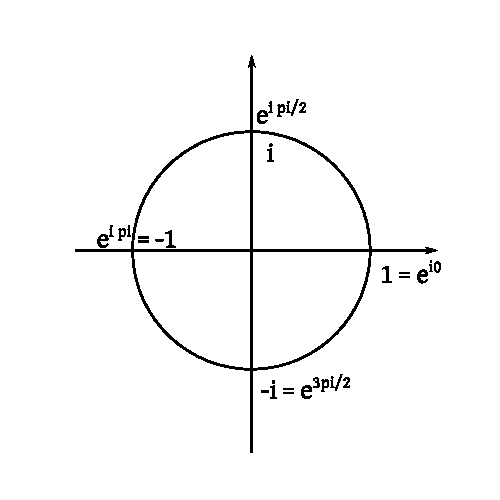
\includegraphics[width=0.4\textwidth]{img/trigonometric-periodicity.pdf}
    \caption{Periodicity of $\cos$ and $\sin$ on the unit circle in the complex plane}
    \label{fig:unitcircle}
  \end{center}
\end{figure}

\begin{rem}
  We will show: $\forall c \in (0, 2\pi)$, $\cos$ and $\sin$ are non-periodic with period $c$,
  hence $\exists x \in \mathbb R$ such that $\cos(x) \neq \cos(x + c)$.
\end{rem}

\index[English]{Periodic function}
\index[German]{\foreignlanguage{ngerman}{Periodische Funktion}}
\index[English]{Period}
\index[German]{\foreignlanguage{ngerman}{Periode}}
\begin{defi}
  $f: \mathbb C \to \mathbb C$ (or $f: \mathbb R \to \mathbb R$)
  is called \emph{periodic} with period $c \in \mathbb C$ ($c \in \mathbb R$)
  if $\forall z \in \mathbb C$ it holds that
  \[ f(z + c) = f(z) \]
  \[ (\text{or } \forall x \in \mathbb R: f(x + c) = f(x)) \]
  $c$ is called \emph{period of $f$}.
\end{defi}

\begin{rem}
  If $f$ is periodic with period $c \in \mathbb C$,
  then $f$ is also periodic with period $k \cdot c$ for every $k \in \mathbb Z \setminus \set{0}$.
\end{rem}

\begin{rem}
  \[ z = u + iv \]
  \[ \Re(i \cdot z) = \Re(i u - v) = -v = - \Im(z) \]
  \[ \Im(i \cdot z) = \Im(iu - v) = u = \Re(z) \]
\end{rem}

\begin{rem}
  Let $x \in \mathbb R$.
  \begin{align*}
    \cos\left(x + \frac\pi2\right)
      &= \Re(e^{i(x + \frac\pi2)}) \\
      &= \Re(e^{ix} \cdot e^{i\frac\pi2}) \\
      &= \Re(i e^{ix}) \\
      &= -\Im(e^{ix}) \\
      &= -\sin(x)
  \end{align*}

  \begin{align*}
    \sin\left(x + \frac\pi2\right)
      &= \Im\left(e^{i(x + \frac\pi2)}\right) \\
      &= \Im(ie^{ix}) \\
      &= \Re(e^{ix}) \\
      &= \cos(x)
  \end{align*}

  \begin{align*}
    \cos\left(x - \frac\pi2\right)
      &= \sin\left(x - \frac\pi2 + \frac\pi2\right) \\
      &= \sin(x)
  \end{align*}

  \begin{align*}
    \sin\left(x - \frac\pi2\right)
      &= -\cos\left(x - \frac\pi2 + \frac\pi2\right) \\
      &= -\cos(x)
  \end{align*}

  Summary:
  \begin{align*}
    \cos\left(x + \frac\pi2\right) &= -\sin(x) \\
    \sin\left(x + \frac\pi2\right) &= \cos(x) \\
    \cos\left(x - \frac\pi2\right) &= \sin(x) \\
    \sin\left(x - \frac\pi2\right) &= -\cos(x)
  \end{align*}
\end{rem}

\begin{rem}[A remark on the name \enquote{cosine}]
  \[ \sin\left(\frac\pi2 - x\right) = -\sin\left(x - \frac\pi2\right) = \cos(x) \]

  \begin{figure}[!h]
    \begin{center}
      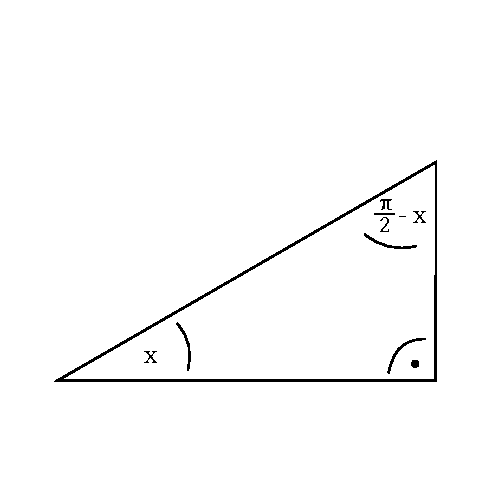
\includegraphics[width=0.4\textwidth]{img/complementary-angle.pdf}
      \caption{Complementary angle: co-sinus}
      \label{img:cosine}
    \end{center}
  \end{figure}

  The sine of the complementary angle is the co-sine of $x$ (Compare with Figure~\ref{img:cosine}).
\end{rem}

\begin{rem}
  \begin{align*}
    \cos(x + \pi) &= \Re(e^{i(x + \pi)}) \\
      &= \Re(-e^{ix}) \\
      &= -\cos(x) \\
    \sin(x + \pi) &= - \sin(x)
  \end{align*}
\end{rem}

\begin{rem}
  Let $0 < c < 2\pi$. Assume $\cos$ is periodic with period $c$.
  We know that $\cos$ has exactly one root in $[0,2]$,
  \[ \cos(x) = \cos(-x) \]
  $\cos$ has exactly two roots in $[-2,2]$, namely $\frac\pi2$ and $-\frac\pi2$.

  \begin{enumerate}
    \item Consider $c \in (0,\pi)$. Then $\cos\left(-\frac\pi2 + c\right) = \cos\left(-\frac\pi2\right) = 0$.
      \[ -\frac\pi2 + c < -\frac\pi2 + \pi = \frac\pi2 < 2 \]
      \[ -\frac\pi2 + c \geq -\frac\pi2 > -2 \]
      Therefore $\cos$ would have another root in $[-2,2]$, namely $-\frac\pi2 + c$.
      This is a contradiction.
    \item
      Consider $c \in [\pi,2\pi)$.
      $c = \pi$ is not a period because $\cos(0) = 1$ and $\cos(0 + \pi) = -1$.
      Let $\pi < c < 2\pi$.
      Then $\frac32 \pi - c < \frac32 \pi - \pi = \frac\pi2$ and $\frac32 \pi - c > \frac32 \pi - 2\pi = -\frac\pi2$.
      Hence,
      \[ \frac32 \pi - c \in \left(-\frac\pi2, \frac\pi2\right) \]
      \[ \cos\left(\frac32 \pi - c\right) = \cos\left(\frac32 \pi - c + c\right) = \cos\left(\frac32 \pi\right) = 0 \]
      $c$ would be the period.
      \[ \Rightarrow \frac32 \pi - c \text{ is a root of $\cos$ in } (-\frac\pi2, \frac\pi2) \]
      This is a contradiction.
  \end{enumerate}

  Therefore it holds that
  \[ \forall c \in (0,2\pi): \exists x \in \mathbb R: \cos(x + c) \neq \cos(x) \]
  Therefore $\cos$ is not periodic with period $c$.
  Hence $2\pi$ is indeed the smallest period of $\cos$.

  Analogously it holds for $\sin$.
\end{rem}

\begin{rem}[Roots of $\cos$]
  \[ \cos\left(\frac\pi2 + 2k\pi\right) = \cos\left(\frac\pi2\right) = 0 \qquad \forall k \in \mathbb Z \]
  \[ \cos\left(\frac32 \pi + 2k \pi\right) = \cos\left(\frac32 \pi\right) = 0 \qquad \forall k \in \mathbb Z \]
  \[ x_k = \frac\pi2 + 2k \pi = \frac{\pi}{2} \left(1 + 4k\right) \]
  \[ y_k = \frac32 \pi + 2k \pi = \frac\pi2 \left(3 + 4k\right) \]
  Hence for $z_l = \frac\pi2 \left(2l + 1\right)$ with $l \in \mathbb Z$ it holds that $\cos(z_l) = 0$.
  These are the odd multiples of $\frac\pi2$.

  \begin{align*}
    \sin(0 + 2k\pi) &= \sin(0) = 0 \\
    \sin(\pi + 2k\pi) &= \sin((2k + 1)\pi) = \sin(\pi) = 0
  \end{align*}
  \[ \Rightarrow (l\pi) = 0 \qquad \forall l \in \mathbb Z \]
\end{rem}

\subsection{Derivatives of trigonometric functions}
%
It holds that
\begin{mdframed}
  \[ \lim_{z \to 0} \frac{\sin{z}}{z} = 1 \]
\end{mdframed}
Furthermore it holds that
\begin{mdframed}
  \[ \lim_{z \to 0} \frac{1 - \cos{z}}{z} = 0 \]
\end{mdframed}

\begin{proof}
  \begin{align*}
    \frac{1 - \cos{z}}{z}
      &= \frac1z \left(1 - 1 + \frac{z^2}{2} - \frac{z^4}{4!} + \frac{z^6}{6!} - \frac{z^8}{8!} + \ldots\right) \\
      &= \frac{z}{2!} - \frac{z^3}{4!} + \frac{z^5}{6!} - \frac{z^7}{8!} + \ldots
  \end{align*}
  is convergent in $\mathbb C$ and (especially) continuous in $0$
  \[ \lim_{z \to 0} \left(\frac{z}{2!} - \frac{z^3}{4!} + \frac{z^5}{6!} - \ldots\right) = 0 \]
\end{proof}

\[
  \lim_{h\to0} \frac{\cos(x + h) - \cos(x)}{h}
\]

\meta{lecture}{11th of March 2016}{Wolfgang Ring}

Recall:
\[ \lim_{z\to0} \frac{\sin{z}}{z} = 1 \]
\[ \lim_{z\to0} \frac{1-\cos{z}}{z} = 0 \]

\begin{lemma}
  The trigonometric functions $\sin$ and $\cos$ are differentiable in $\mathbb R$
  (because they can be expressed as power series with infinite convergence radius)
  and it holds that
  \[ \cos'(x) = -\sin(x)  \qquad  \sin'(x) = \cos(x) \]
\end{lemma}
\begin{proof}
  \begin{align*}
    \lim_{h\to0} \frac{\cos(x + h) - \cos(h)}{h}
      &= \lim_{h\to0} \frac{\cos{x} \cdot \cos{h} - \sin{x} \cdot \sin{h} - \cos{x}}{h} \\
      &= \lim_{h\to0} \cos{x} \cdot \frac{\cos(h) - 1}{h} - \lim_{h\to0} \frac{\sin{x} \cdot \sin{h}}{h} \\
      &= \cos{x} \cdot \underbrace{\lim_{h\to0} \frac{\cos(h) - 1}{h}}_{=0} - \sin{x} \cdot \underbrace{\lim_{h\to0} \frac{\sin(h)}{h}}_{=1} \\
      &= -\sin(x)
  \end{align*}

  Analogously:
  \begin{align*}
    \lim_{h\to0} \frac{\sin(x + h) - \sin(h)}{h}
      &= \lim_{h\to0} \frac{\sin{x} \cdot \cos{h} + \sin{h} \cdot \cos{x} - \sin{x}}{h} \\
      &= \sin(x) \cdot \underbrace{\lim_{h\to0} \frac{\cos(h) - 1}{h}}_{=0} + \cos(x) \cdot \underbrace{\lim_{h\to0} \frac{\sin{h}}{h}}_{=1} \\
      &= \cos(x)
  \end{align*}
\end{proof}
\begin{figure}[!h]
  \begin{center}
    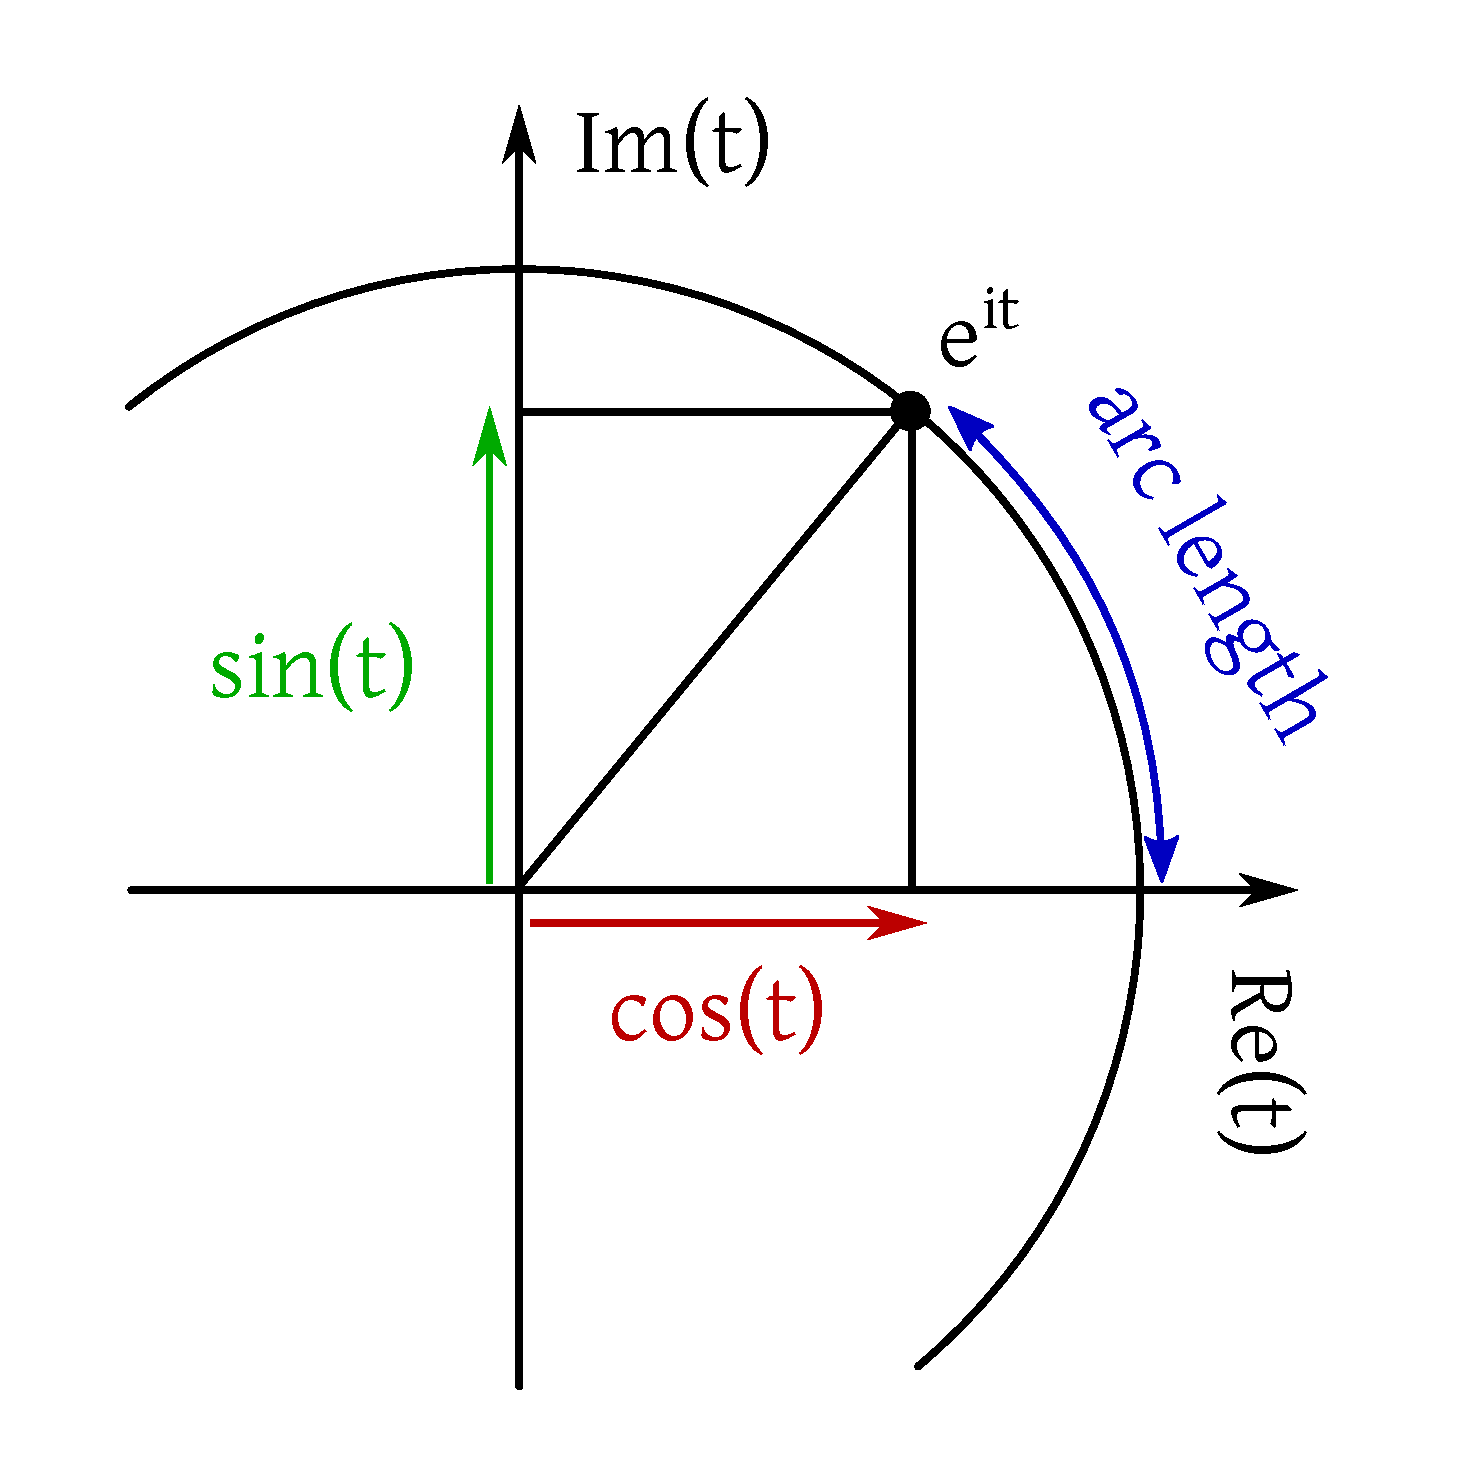
\includegraphics[width=0.3\textwidth]{img/arclength_on_unitcircle.pdf}
    \caption{The arc length is related to $\sin$ and $\cos$}
    \label{img:arc-length}
  \end{center}
\end{figure}

Compare with Figure~\ref{img:arc-length}. We now use tools of integral calculus:

Let $I = [a,b]$ and $\gamma: I \to \mathbb R^n$ ($\mathbb R^2$).
\[ \gamma(t) = \begin{bmatrix} \gamma_1(t) \\ \vdots \\ \gamma_n(t) \end{bmatrix} \]
Assumption: $\gamma_1: [a,b] \to \mathbb R^n$ is continuously differentiable.

\[ \gamma'(t) = \begin{bmatrix} \gamma'_1(t) \\ \vdots \\ \gamma'_n(t) \end{bmatrix} \]
is the tangential vector in $\gamma$. Compare with Figure~\ref{img:tangentialvector}.

\begin{figure}[!h]
  \begin{center}
    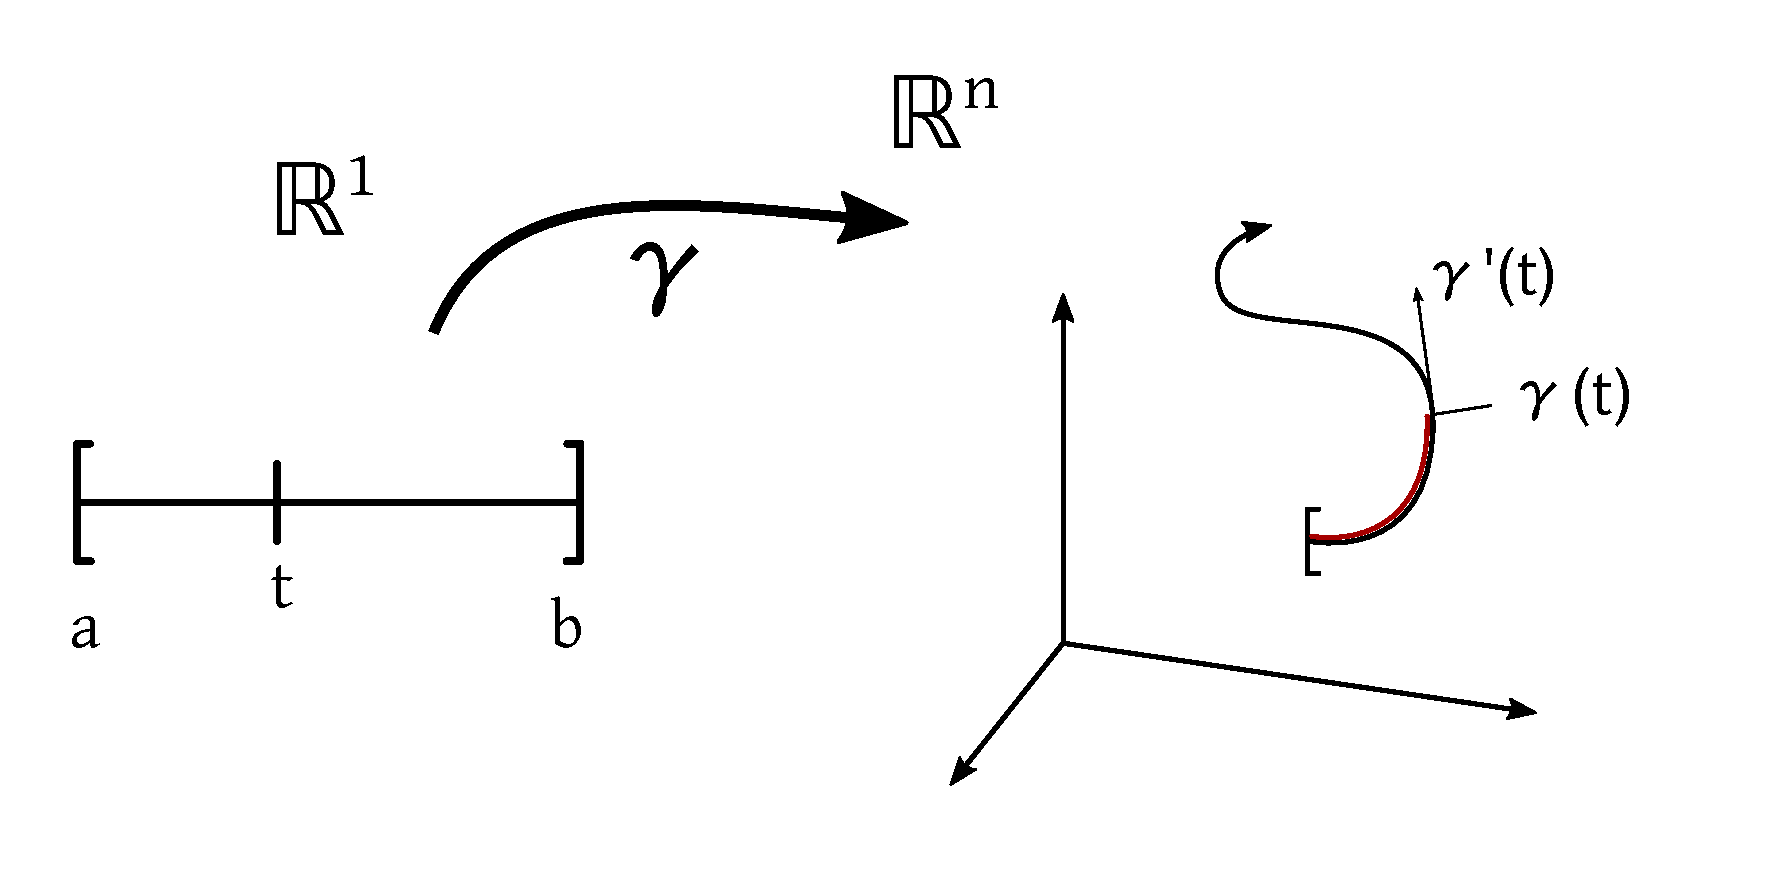
\includegraphics[width=0.4\textwidth]{img/curve_mapped.pdf}
    \caption{Mapping of the curve and tangential vector $\gamma'(t)$}
    \label{img:tangentialvector}
  \end{center}
\end{figure}

Let $t \in [a,b]$. Then the arc length of $\gamma$ between $a$ and $t$
is given by
\[ S(t) = \int_a^t \abs{\gamma'(\tau)} \, d\tau \]

We identify $\mathbb C$ with $\mathbb R^2$:
\[ x + iy \leftrightarrow \begin{bmatrix} x \\ y \end{bmatrix} \]

\[ \gamma: t \mapsto e^{it} = \cos{t} + i \cdot \sin{t} \]
is a curve in $\mathbb C \cong \mathbb R^2$.
\[ \gamma: [0,2\pi] \to \mathbb C \]

\[ \gamma(t) = \begin{bmatrix} \cos{t} \\ \sin{t} \end{bmatrix} \]
\[ \gamma'(t) = \begin{bmatrix} -\sin{t} \\ \cos{t} \end{bmatrix} \]

\begin{figure}[!h]
  \begin{center}
    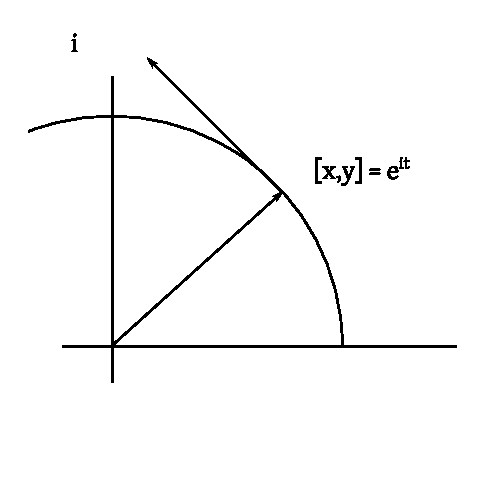
\includegraphics{img/derivative-in-r2.pdf}
    \caption{Derivative in $\mathbb R^2$}
    \label{img:deriv-r2}
  \end{center}
\end{figure}

Compare with Figure~\ref{img:deriv-r2}.
\[ \abs{\gamma'(t)} = \sqrt{(-\sin(t))^2 + (\cos(t))^2} = 1 \]
\[ \int_0^t \abs{\gamma'(\tau)} \, d\tau = \int_0^t 1 \, d\tau = t \]

\section{Integral calculus}
%
Integration calculus was developed to determine areas of curves regions.
It was developed by Leibniz, Cauchy, Riemann and Lebeque. There are different
notions of integrations and it will discussed in further details in the courses
\enquote{Functional analysis} and \enquote{Measure and integration theory}.
For now, we look at the basics (as discussed by \foreignlanguage{ngerman}{Königsberger}).

\index[English]{Step function}
\index[German]{\foreignlanguage{ngerman}{Treppenfunktion}}
\begin{defi}[Step function]
  Let $[a,b]$ be an interval, $a,b \in \mathbb R$ with $a<b$ and $\phi: [a,b] \to \mathbb R$.
  We call $\varphi$ a \emph{step function}, if $n \in \mathbb N$ and $x_0, \ldots, x_n$
  exist such that
  \[ x_0 = a < x_1 < x_2 < \ldots < x_n = b \]
  and $\varphi|_{(x_{j-1}, x_j)} = c_j$ is constant.
  The points $x_j$ define a partition of the interval $[a,b]$.
\end{defi}

$\tau[a,b]$ defines the set of step functions of interval $[a,b]$.
The function values defining the partitions do not have any constraints and
are therefore irrelevant for further considerations (compare with Figure~\ref{img:partition-int}).

\begin{figure}[!h]
  \begin{center}
    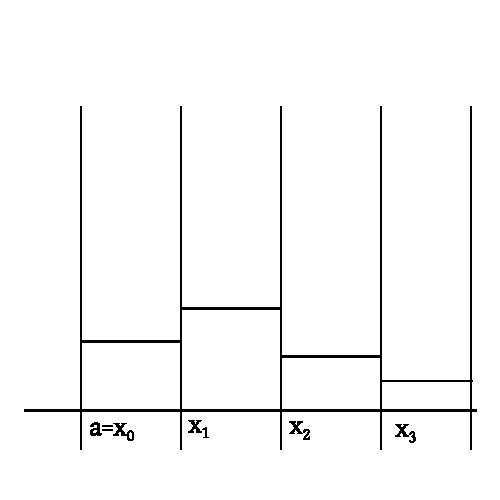
\includegraphics{img/partition-of-integral.pdf}
    \caption{Partition of an area into rectangles}
    \label{img:partition-int}
  \end{center}
\end{figure}

\index[English]{Integral}
\index[German]{\foreignlanguage{ngerman}{Integral}}
\begin{defi}[Integral]
  Let $\varphi:[a,b] \to \mathbb R$ be a step function and
  $x_0 = a < x_1 < \ldots < x_n = b$ a partition of
  $[a,b]$ and let $\varphi|_{(x_{j-1}, x_j)} = c_j$
  for $j = 1,\ldots,n$.
  Then we define
  \[ \int_a^b \varphi \,dx = \sum_{j=1}^n c_j \triangle x_j \]
  where
  $\triangle x_j = x_j - x_{j-1}$ (for $j=1,\ldots,n$).
  \[ \int_a^b \varphi \, dx \text{ is called \emph{integral} of $\varphi$ over $[a,b]$} \]
\end{defi}

$\varphi$ is the step function in terms of the partition $\set{x_0,x_1,\ldots, x_5}$,
but also a step function in terms of $\set{w_0, w_1, \ldots, w_5}$.

It remains to show that if $\varphi$ satisfies the definition of a step function in terms of
partition $\set{x_0,\ldots,x_n}$ and $\varphi|_{(x_{j-1}, x_j)} = c_j$
and $\varphi$ is a step function in terms of $\set{w_0,w_1,\ldots,w_m}$
and $\varphi|_{(w_{l-1},w_l)} = c'_l$, then it holds that
\[ \sum_{j=1}^n c_j \triangle x_j = \sum_{l=1}^m c'_l \triangle w_l \]
Compare with Figure~\ref{img:step-function}.

\begin{figure}[!h]
  \begin{center}
    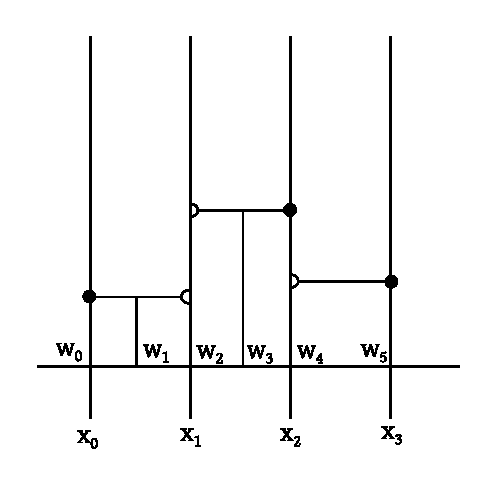
\includegraphics{img/step-function.pdf}
    \caption{Step function $\varphi$}
    \label{img:step-function}
  \end{center}
\end{figure}

\begin{proof}
  Let $Z = \set{x_0, \ldots, x_n}$ and $Z' = \set{w_0,\ldots,w_m}$.
  We define $Z'' = Z \cup Z'$ and $Z'' = \set{\alpha_0, \alpha_1, \ldots, \alpha_L}$.
  Duplicates get lost in the set.
  \[ \alpha_0 = a < \alpha_1 < \ldots < \alpha_L = b \]
  Because $Z \subseteq Z''$,
  \[ \forall x_j \exists k_j: x_j = \alpha_{k_j} \]
  Because $x_{j-1} < x_j$, it holds that $\alpha_{k_{j-1}} < \alpha_{k_j}$.
  Followingly, $k_{j-1} < k_j$.
  Now let $k_{j-1} < l \leq k_j$.
  It holds that $(\alpha_{l-1}, \alpha_l) \subseteq (x_{j-1}, x_j)$,
  because $l > k_{j-1} = l-1 \geq k_{j-1} \Rightarrow \alpha_{l-1} \geq \alpha_{k_{j-1}} = x_{j-1}$
  and $l \leq k_j$.
  \[ \Rightarrow \alpha_l \leq \alpha_{k_j} = x_j \]
  So for $x \in (\alpha_{l-1}, \alpha_l) \subseteq (x_{j-1}, x_j)$ it holds that
  $\varphi(x) = c_j$.

  $k_0 = 0$ because $x_0 = \alpha_0 = a$ and $k_n = L$ because $x_n = \alpha_L = b$.
  $\forall l \in \set{0,\ldots,L}$ there exists $j \in \set{1,\ldots,n}$ such that
  $k_{j-1} \leq l \leq k_j$.

  \[ \Rightarrow \varphi|_{(\alpha_{l-1},\alpha_l)} \text{ is constant} \]

  Hence $\varphi$ is a step function in terms of the partition $\set{\alpha_0, \ldots, \alpha_L}$.

  Let $l \in \set{0,1,\ldots,L}$ and $j$ such that
  \[ k_{j-1} < l \leq k_j \Rightarrow (\alpha_{l-1},\alpha_l) \subset (x_{j-1},x_j) \]
  and $c''_l = \varphi(x)$ for $x \in (\alpha_{l-1},\alpha_l)$, then $c''_l = c_j$.

  \[ \sum_{l=1}^L c''_l \cdot \triangle \alpha_l = \sum_{j=1}^n \sum_{l=k_{j-1}+1}^{k_j} c''_l \triangle \alpha_l \]
  \[ = \sum_{j=1}^n c_j \sum_{l=k_{j-1}+1}^{k_j} \triangle \alpha_l = \sum_{j=1}^n c_j \triangle x_j \]
  Because
  \[
    \sum_{l=k_{j-1} + 1}^{k_j} \triangle \alpha_l
    = (\alpha_{k_{j-1}+1} - \alpha_{k_{j-1}}) + (\alpha_{k_{j-1}+2} - \alpha_{k_{j-1}+1})
  \] \[
    + (\alpha_{k_{j-1}+3} - \alpha_{k_{j-1}+2}) + \ldots + (\alpha_{k_j-1} - \alpha_{k_j-2}) + (\alpha_{k_j} - \alpha_{k_j-1})
  \]
  This is a telescoping sum. What remains is:
  \[ = \alpha_{k_j} - \alpha_{k_{j-1}} \]

  \[ x_j - x_{j-1} = \triangle x_j \]
  Analogously,
  \[ \sum_{l=1}^L c''_l \cdot \triangle \alpha_l = \sum_{k=1}^m c'_k \triangle w_k \]
  So it holds that
  \[ \sum_{j=1}^n c_j \triangle x_j = \sum_{k=1}^m c'_k \triangle w_k \]
\end{proof}

\meta{lecture}{15th of March 2016}{Wolfgang Ring}

\begin{lemma}
  Let $\varphi \in \tau[a,b]$ be a step function in terms of partition
  $a = x_0 < x_1 < \ldots < x_n = b$.
  Let $a = \alpha_0 < \alpha_1 < \ldots < \alpha_L = b$ with
  $Z = \set{x_0, \ldots, x_n} \subseteq \set{\alpha_0, \alpha_1, \ldots, \alpha_L} = z'$
  ($z'$ has more intervals than $Z'$).

  Then also $\varphi$ is step function in terms of partition $z'$.
\end{lemma}

\begin{proof}
  See above.
\end{proof}

\index[English]{Linearity of integration}
\index[German]{\foreignlanguage{ngerman}{Linearität des Integral}}
\begin{lemma}
  Let $\varphi_1, \varphi_2 \in \tau[a,b]$ and $\alpha, \beta \in \mathbb C$.

  Then it holds that
  \begin{itemize}
    \item $\alpha \varphi + \beta \psi \in \tau[a,b]$ and
      \[ \int_a^b (\alpha \varphi + \beta \psi) \, dx = \alpha \int_a^b \varphi \, dx + \beta \int_a^b \psi \, dx \]
      Hence (\enquote{linearity}),
      \[ \int_a^b: \tau[a,b] \to \mathbb R \text{ is linear} \]
    \item $\abs{\varphi} \in \tau[a,b]$ and it holds that
      \[ \abs{\int_a^b \varphi \, dx} \leq \int_a^b \abs{\varphi} \, dx \leq \norm{\varphi}_\infty (b-a) \]
      Reminder: $\norm{\varphi}_\infty = \max\set{\abs{\varphi(x)}: x \in [a,b]}$ \\
      This gives \enquote{boundedness}.
    \item Let $\varphi$ and $\psi$ be real values and it holds that
      \[ \forall x \in [a,b]: \varphi(x) \leq \psi(x) \]
      Hence monotonicity is given.
      Then it holds that
      \[ \int_a^b \varphi \, dx \leq \int_a^b \psi \, dx \]
  \end{itemize}
\end{lemma}
\begin{proof}
  \begin{itemize}
    \item Let $\varphi|_{(x_{k-1},x_k)} = c_k$ $\psi|_{(w_{j-1},w_j)} = d_k$
      \[ z'' = \set{\alpha_0, \alpha_1, \ldots, \alpha_L} = \set{x_0, \ldots, x_n} \cup \set{w_0, \ldots, w_m} \]
      where $\alpha_i$ is sorted ascendingly.
      $\varphi$ and $\psi$ are step functions in terms of $z''$, hence
      \[ \varphi|_{(\alpha_{i-1},\alpha_i)} = c_i' \text{ and } \psi|_{(\alpha_{i-1},\alpha_i)} = d'_i \]
      \[ \Rightarrow (\alpha \varphi + \beta \psi) |_{(\alpha_{i-1},\alpha_i)} = \alpha c_i' + \beta d_i' \text{ constant} \]
      \[ \Rightarrow \alpha \varphi + \beta \psi \in \tau[a,b] \text{ and } \int_a^b (\alpha \varphi + \beta \psi) \, dx = \sum_{i=1}^L (\alpha c'_i + \beta d'_i) \cdot \triangle \alpha_i \]
      \[ = \alpha \sum_{i=1}^L c'_i \triangle \alpha_i + \beta \sum_{i=1}^L d_i' \triangle \alpha_i \]
      \[ = \alpha \int_a^b \varphi \, dx + \beta \int_a^b \psi \, dx \]
    \item
      Let $\varphi|_{(x_{i-1},x_i)} = c_i$ ($i = 1, \ldots, n$). Then,
      \[ \abs{\varphi} |_{(x_{i-1},x_i)} = \abs{c_i} \]
      \[
        \abs{\sum_{i=1}^n c_i \triangle x_i}
        \leq \sum_{i=1}^n \abs{c_i} \cdot \underbrace{\abs{\triangle x_i}}_{x_i - x_{i-1} > 0}
        = \sum_{i=1}^n \abs{c_i} \cdot \triangle x_i = \int_a^b \abs{\varphi} \, dx
      \]
      \[
        \leq \sum_{i=1}^n \norm{\varphi}_\infty \triangle x_i
        = \norm{\varphi}_\infty \sum_{i=1}^n \triangle x_i
      \] \[
        = \norm{\varphi}_\infty \left((x_1 - x_0) + (x_2 - x_1) + \ldots + (x_{n-1} - x_{n-2}) + (x_n - x_{n-1})\right)
      \] \[
        = \norm{\varphi}_\infty (x_n - x_0) = \norm{\varphi}_\infty (b-a)
      \]
    \item
      Let $\varphi$, $\psi$ and $z''$ as in the linearity statement.
      \[
        \left.\begin{array}{rl}
          \varphi|_{(\alpha_{i-1},\alpha_i)} &= c'_i \in \mathbb R \\
          \psi|_{(\alpha_{i-1}, \alpha_i)} &= d'_i \in \mathbb R
        \end{array}\right\}
      \] \[
        \int_a^b \varphi \, dx = \sum_{i=1}^L c'_i \underbrace{\triangle \alpha_i}_{>0} \leq \sum_{i=1}^L d'_i \, dx
      \] \[
        \int_a^b \varphi \, dx
      \]
  \end{itemize}
\end{proof}
\index[English]{Characteristic function}
\index[German]{\foreignlanguage{ngerman}{Charakteristische Funktion}}
\begin{defi}
  Let $A \subseteq \mathbb R$. Then we call $\chi_A = (\mathcal 1_A): \mathbb R \to \mathbb R$ as
  \[ \chi_A(x) = \begin{cases} 1 & x \in A \\ 0 & x \not\in A \end{cases} \]
  the \emph{characteristic function of $A$}. Hence $\chi_A(x)$ is $1$ if and only if $x$ is inside interval $A$.
\end{defi}
\begin{rem}
  Let $a \leq a' < b' \leq b$. Then
  \[ \chi_{(a',b')} \in \tau[a,b] \qquad \int_a^b \chi_{(a',b')} \, dx = 1 \cdot (b' - a') \]
  Every linear combination of characteristic functions is also in $\tau[a,b]$.

  On the opposite side, let $\varphi \in \tau[a,b]$ with $\varphi|_{(x_{i-1},x_i)} = c_i$
  and $\varphi(x_i) \eqqcolon r_j$ with $1 \leq i \leq n$ and $0 \leq j \leq n$.
  \[
    \Rightarrow \varphi = \sum_{i=1}^n c_i \chi_{(x_{i-1},x_i)}
    + \sum_{j=0}^n r_j \chi_{\set{x_j}}
  \]
  The step function is a linear combination of characteristic functions
  of open intervals and of characteristic functions of one-point sets.
  \[
    \int_a^b \varphi \, dx
    = \sum_{i=1}^n c_i \cdot (x_i - x_{i-1})
    = \sum_{i=1}^n c_j \int_a^b \chi_{(x_{i-1},x_i)} \, dx
  \]
\end{rem}

\section{Regulated functions}

\index[English]{Left-sided limit}
\index[German]{\foreignlanguage{ngerman}{Linksseitiger Grenzwert}}
\index[English]{Right-sided limit}
\index[German]{\foreignlanguage{ngerman}{Rechtsseitiger Grenzwert}}
\index[English]{One-sided limit}
\index[German]{\foreignlanguage{ngerman}{Einseitiger Grenzwert}}
\begin{defi}
  Let $D \subseteq \mathbb R$. Let $x_0$ be a limit point of $D \cap (-\infty, x_0)$
  hence $\exists (z_n)_{n \in \mathbb N}$ with $z_n \in D \cap (-\infty, x_0)$,
  hence $z_n < x_0$, and $\lim_{n\to\infty} z_n = x_0$.
  Let $f: D \to \mathbb C$ be given.

  We state that $f$ has left-sided limit $y_0$ in $x_0$ if
  \[ \forall \varepsilon > 0 \exists \delta > 0: \left[x \in D \cap (-\infty, x_0) \land \abs{x - x_0} < \delta \right] \]
  \[ \Rightarrow \abs{f(x) - y_0} < \varepsilon \]

  Equivalently $\forall (z_n)_{n\in\mathbb N}$ with $z_n \in D$
  and $z_n < x_0$ and $\lim_{n\to\infty} z_n = x_0$ $\forall n \in \mathbb N$
  \[ \lim_{n\to\infty} f(x_n) = y_0 \]

  Analogously for the right-sided limes, we replace $(-\infty, x_0)$ by $(x_0, \infty)$.

  We denote: $y_0$ is left-sided limit of $f$ in $x_0$:
  \[ y_0 = \lim_{x\to x_0^-} f(x) \]
  and right-sided limit of $f$ in $x_0$:
  \[ y_0 = \lim_{x\to x_0^+} f(x) \]
\end{defi}

\index[English]{Regulated function}
\index[German]{\foreignlanguage{ngerman}{Regelfunktion}}
\begin{defi}
  Let $a,b \in \mathbb R$ and $a < b$. A function $f: [a,b] \to \mathbb C$ is called
  \emph{regulated functions} if
  \begin{itemize}
    \item $\forall x \in (a,b)$ $f$ has a left-sided and a right-sided limes in $x$
    \item $f$ has a right-sided limes in $a$
    \item $f$ has a left-sided limes in $b$
  \end{itemize}
\end{defi}

Examples for regulated functions:
\begin{itemize}
  \item Every continuous function in $[a,b]$ is a regulated function.
  \item Every step function is a regulated function. \\
    Why? Consider $x \in (x_{i-1},x_i)$. Then
    \[ \lim_{\xi\to x^+} \varphi(\xi) = c_i = \lim_{\xi \to x^-} \varphi(\xi) \]
    Let $x = x_i$ be a partitioning point.
    \[ \lim_{\xi \to x_i^-} \varphi(\xi) = c_i \text{ and } \lim_{\xi \to x_i^+} \varphi(\xi) = c_{i+1} \]
    So $\tau[a,b] \subseteq R[a,b]$. Compare with Figure~\ref{img:step-regulated}.
  \item
    Let $f: [a,b] \to \mathbb R$ be monotonically.
    Then it holds that
    \[ f \in R[a,b] \]
\end{itemize}

\begin{figure}[!h]
  \begin{center}
    \fbox{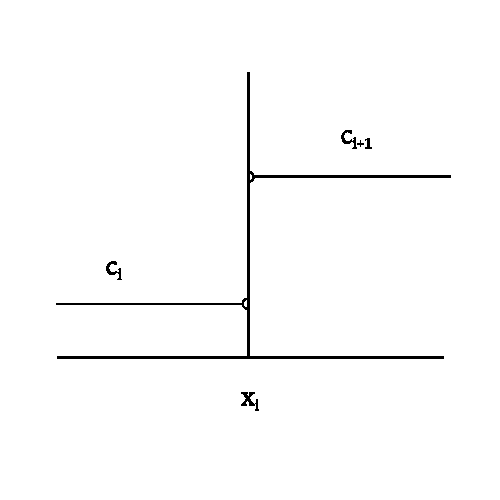
\includegraphics{img/step-functions-are-regulated-functions.pdf}}
    \caption{Step functions are also regulated functions}
    \label{img:step-regulated}
  \end{center}
\end{figure}

\subsection{Approximation theorem for regulated functions}

Let $f: [a,b] \to \mathbb C$. Then it holds that $f \in R[a,b] \Leftrightarrow \forall \varepsilon > 0 \exists \varphi \in \tau[a,b]$ such that $\norm{f - \varphi}_{\infty} < \varepsilon$. Hence,
\[ \forall x \in [a,b]: \abs{f(x) - \varphi(x)} < \varepsilon \]
\[ \Leftrightarrow \underbrace{\sup\set{\abs{f(x) - \varphi(x)}: x \in [a,b]}}_{\norm{f - \varphi}_{\infty}} < \varepsilon \]

Especially $\varepsilon_n = \frac1n \Rightarrow \exists \varphi_n \in \tau[a,b]$ such that
\[ \abs{\varphi_n(x) - f(x)} < \varepsilon \qquad \forall x \in [a,b] \]
hence $f$ is a continuous limit point of a sequence of step functions.
Hence the function sequence $(\varphi_n)_{n\in\mathbb N}$ converges continuously towards $f$.

\begin{proof}
  \begin{description}
    \item[$\Rightarrow$]
      Let $f \in R[a,b]$.
      Assume $\exists \varepsilon > 0$ fixed such that $\forall \varphi \in \tau[a,b]$
      \[ \exists x \in [a,b]: \abs{\varphi(x) - f(x)} \geq \varepsilon \]
      We build nested intervals such that the desired property $\abs{\varphi(x) - f(x)} \geq \varepsilon$
      holds on every subinterval $[a_n, b_n]$.

      Induction:
      \begin{description}
        \item[$n=0$] Let $a_0 = a$ and $b_0 = b$, hence the property holds in $[a_0, b_0]$.
        \item[$n\mapsto n+1$]
        Let $m = \frac12 (a_n + b_n)$. In $[a_n,b_n]$ the property holds.

        Then the property either holds in $[a_n,m]$ or $[m,b_n]$.
        If the property does not hold in $[a_n,m]$:
        \[ \exists \varphi_1 \in \tau[a_n,m] \text{ with } \abs{\varphi_1(\xi) - f(\xi)} < \varepsilon \qquad \forall \xi \in [a_n,m] \]
        If the property does not hold in $[m,b_n]$:
        \[ \exists \varphi_2 \in \tau[m,b_n] \text{ with } \abs{\varphi_2(\xi) - f(\xi)} < \varepsilon \qquad \forall \xi \in [m,b_n] \]
        Let
        \[
          \varphi(x) = \begin{cases}
            \varphi_1(x) & \text{ for } x \in [a_n,m] \\
            \varphi_2(x) & \text{ for } x \in [m,b_n]
          \end{cases}
        \]
        \[ \Rightarrow \varphi \in \tau[a,b] \text{ and } \abs{\varphi(\xi) - f(\xi)} < \varepsilon \qquad \forall \xi \in [a_n,b_n] \]
        So in at least one of the intervals the property holds.
        Let this interval be $[a_{n+1},b_{n+1}]$.

        $([a_n,b_n])_{n\in \mathbb N}$ are nested intervals.
        Let $\varphi \in \bigcap_{n \in \mathbb N} [a_n, b_n]$.

        \begin{description}
          \item[Case $\mathbf{\xi \in (a,b)}$]
            Let $\varepsilon$ satisfy the desired property.
            $f \in R[a,b]$, hence $f$ has left-sided limit $c_-$ in $\xi$
            and right-sided limit $c_+$. Hence $\exists \delta > 0$ such that
            \begin{itemize}
              \item $\abs{x - \xi} < \delta \land a \leq x < \xi
              \Rightarrow \abs{f(x) - c_-} < \varepsilon$
              \item $\abs{x - \xi} < \delta \land \delta < x \leq b
              \Rightarrow \abs{f(x) - c_+} < \varepsilon$
            \end{itemize}
            Choose $\delta$ sufficiently small such that
            \[ a < \xi - \delta < \xi + \delta < b \]
            Let
            \[
              \varphi(x) = \begin{cases}
                c_- & \text{ for } x \in (\xi - \delta, \xi) \\
                f(\xi) & \text{ for } x = \xi \\
                c_+ & \text{ for } x \in (\xi, \xi + \delta)
              \end{cases}
            \]
            $\varphi$ is necessarily a step function in $(\xi - \delta, \xi + \delta)$
            and it holds that $\forall x \in (\xi - \delta, \xi + \delta):
            \abs{\varphi(x) - f(x)} < \varepsilon$.

            Let $n$ be sufficiently large such that
            \[ [a_n,b_n] \subseteq (\xi - \delta, \xi + \delta) \]
            then
            \[
              \varphi|_{[a_n,b_n]} \in \tau[a_n,b_n]
              \text{ and }
              \abs{\varphi(x) - f(x)} < \varepsilon \quad \forall x \in [a_n,b_n]
            \]
            This is a contradiction to our desired property.
        \end{description}

        For $\xi = a$ or $\xi = b$ only with one-sided limit.
      \end{description}
  \end{description}
\end{proof}

\meta{lecture}{17th of March 2016}{Wolfgang Ring}

We learned: All regulated functions can be approximated with step functions.

$f \in R[a,b]$ in the proof $\Leftrightarrow$ $f$ is uniform limit of step functions.
We have prove direction $\Rightarrow$.

\begin{lemma}[Cauchy criterion for limits of functions]
  Let $f: D \subseteq \mathbb C \to \mathbb C$ and $z_0$ is a limit point
  of $D$. Then $f$ has a limit in $z_0$ if and only if $\forall \varepsilon > 0
  \exists \delta > 0: v,w \in D\setminus\set{z_0} \land \abs{v - z_0} < \delta \land
  \abs{w - z_0} < \delta \Rightarrow \abs{f(v) - f(w)} < \varepsilon$.

  If $D \subseteq \mathbb R$ and $x_0$ is limit point of $D \cap (x_0, \infty)$,
  then $f$ has a \emph{right-sided limit} in $x_0$ if and only if
  $\forall \varepsilon > 0 \exists \delta > 0: [v,w \in D \cap (x_0, \infty)
  \land \abs{v - x_0} < \delta \land \abs{w-x_0} < \delta \Rightarrow
  \abs{f(v) - f(w)} < \varepsilon]$.

  Analogously for left-sided limit.
\end{lemma}
\begin{proof}
  This proof is done only for the first point.

  \begin{description}
    \item[$\Rightarrow$] \hfill{} \\
      Assume $f$ has a limit $\eta$ in $z_0$. Choose $\delta$ such that $v,w \in D$
      with $\abs{v - z_0} < \delta$ and $\abs{w - z_0} < \delta$ implies
      that $\abs{f(v) - \eta} < \frac\varepsilon2$ and $\abs{f(w) - \eta} < \frac\varepsilon2$.
      Then $\abs{f(v) - f(w)} \leq \abs{f(v) - \eta} + \abs{\eta - f(w)}
      \leq \frac\varepsilon2 + \frac\varepsilon2 = \varepsilon$.
    \item[$\Leftarrow$] \hfill{} \\
      Assume the Cauchy criterion holds. Show: There exists $\eta \in \mathbb C$
      such that for every sequence $(w_n)_{n \in \mathbb N}$
      with $w_n \in D \setminus \set{z_0}$ with $\lim_{n\to\infty} w_n = z_0$
      it holds that $\lim_{n\to\infty} f(w_n) = \eta$.

      Let $(w_n)_{n\in\mathbb N}$ be as above. Show: $(f(w_n))_{n\in\mathbb N}$
      is a Cauchy sequence. Let $\varepsilon > 0$ be given and $\delta$ as above.
      Choose $N \in \mathbb N$ such that $n,m \geq N$
      \[ \Rightarrow \abs{w_n - z_0} < \delta \land \abs{w_m - z_0} < \delta \]
      The Cauchy criterion holds for $n,m \geq N$:
      \[ \abs{f(w_n) - f(w_m)} < \varepsilon \]
      So $(f(w_n))_{n \in \mathbb N}$ is a Cauchy sequence and (because $\mathbb C$ is complete)
      is also convergent.
      So $\exists \eta' \in \mathbb C: \lim_{n\to\infty} f(w_n) = \eta'$.

      It remains to show: $\eta'$ is unique.

      Let $(v_n)_{n\in\mathbb N}$ be another sequence with $\lim_{n\to\infty} v_n = z_0$
      and $v_n \in D \setminus \set{z_0}$. As above: $\exists \eta'' \in \mathbb C$ such that
      $\lim_{n\to\infty} f(v_n) = \eta''$.

      We construct:
      \[ (\xi_n)_{n\in\mathbb N} = (w_0, v_0, w_1, v_1, w_2, v_2, \ldots) \]
      Then it holds that $\lim_{n\to\infty} \xi_n = z_0$.

      We use the argument from above: $(f(\xi_n))_{n\in\mathbb N}$ is convergent,
      hence $\lim_{n\to\infty} f(\xi_n) = \eta$.
      Both subsequences $(f(w_n))_{n\in\mathbb N}$ and $(f(v_n))_{n\in\mathbb N}$
      must have the same limit, hence $\eta' = \eta = \eta''$.
  \end{description}
\end{proof}

\begin{proof}[Proof of approximation theorem]
  \begin{description}
    \item[$\Leftarrow$] \hfill{} \\
      Let $f = \lim_{n\to\infty} \varphi_n$ be uniform on $[a,b]$.
      Let $\varphi_n \in \tau[a,b]$ and let $x_0 \in [a,b)$.
      Show: $f$ has a right-sided limit in $x_0$.
      Let $\varepsilon > 0$ arbitrary. Choose $N \in \mathbb N$ sufficiently
      large such that
      \[
        \abs{f(x) - \varphi_N(x)} < \frac\varepsilon2
        \forall x \in [a,b]
      \]
      $\varphi_N$ is a step function (hence interval-wise constant).
      Choose $\delta > 0$ such that $\varphi_N|_{(x_0,x_0 + \delta)} = c$
      constant. Let $v,w \in (x_0, x_0 + \delta)$. Then it holds that
      \[ \abs{f(v) - f(w)} \leq \abs{f(v) - c} + \abs{c - f(w)} \]
      \[
        = \abs{f(v) - \varphi_N(v)} + \abs{f(w) - \varphi_N(w)}
        < \frac\varepsilon2 + \frac\varepsilon2 = \varepsilon
      \]
      The Cauchy criterion implies that $f$ has a right-sided limit in $x_0$.
  \end{description}
\end{proof}

\begin{cor}
  $f \in R[a,b]$ if and only if $f(x) = \sum_{j=0}^\infty \psi_j(x)$ with
  $\psi_j \in \tau[a,b]$ and the series converges uniformly in $[a,b]$.
\end{cor}
\begin{proof}
  \begin{description}
    \item[$\Leftarrow$] \hfill{} \\
      Let $\varphi_n = \sum_{j=0}^n \psi_j \in \tau[a,b]$ and $\varphi_n \to f$
      continuously in $[a,b]$. From the approximation theorem it follows that
      $f \in R[a,b]$.
    \item[$\Rightarrow$] \hfill{} \\
      Let $f \in R[a,b]$. Let $(\varphi_n)_{n \in \mathbb N}$ be a sequence of step
      functions with $\varphi_n \to f$ uniform in $[a,b]$. Let $\psi_0 = \varphi_0$.
      \[ \psi_j \coloneqq \varphi_j - \varphi_{j-1} \text{ for } j \geq 1 \]
      Then it holds that
      \[
        \sum_{j=0}^n \psi_j = \varphi_0 + (\varphi_1 - \varphi_0) +
          (\varphi_2 - \varphi_1) + \ldots + (\varphi_{n-1} - \varphi_{n-2}) +
          (\varphi_n - \varphi_{n-1})
        = \varphi_n
      \]
      and $(\varphi_n)_{n\in\mathbb N}$ converges uniform if and only if
      the series is uniformly convergent.
  \end{description}
\end{proof}

\begin{lemma}[Sidenote]
  \label{lemma-cont-func-seq}
  Let $(f_n)_{n\in\mathbb N}$ with $f_n: D \to \mathbb C$ a sequence of functions
  in $D$, let $z_0 \in D$ and $\forall n \in \mathbb N$ $f_n$ is continuous in $z_0$.
  Furthermore let $f: D \to \mathbb C$ and $f_n \to f$ is uniform in $D$.
  Then $f$ is continuous in $z_0$.
\end{lemma}
\begin{proof}
  Let $\varepsilon > 0$ arbitrary. Choose $N$ sufficiently large such that
  $\abs{f(z) - f_w(z)} < \frac\varepsilon3 \quad \forall z \in D$ (uniform convergence).
  Because $f_N$ is continuous in $z_0$, $\exists \delta > 0$ such that
  $z \in D$ and $\abs{z - z_0} < \delta$ then $\abs{f_N(z) - f_N(z_0)} < \frac\varepsilon3$.

  Then for $\abs{z - z_0} < \delta$ (with $z \in D$)
  \[
    \underbrace{\abs{f(z) - f(z_0)}}_{< \frac\varepsilon3} \leq
    \underbrace{\abs{f(z) - f_N(z)} + \abs{f_N(z) - f_N(z_0)}}_{< \frac\varepsilon3} +
    \underbrace{\abs{f_N(z_0) - f(z_0)}}_{< \frac\varepsilon3}
  \]
\end{proof}

\meta{lecture}{18th of March 2016}{Wolfgang Ring}

\begin{theorem}
  Let $f$ be a regulated function in $[a,b]$.
  Then $f$ is in at most countable infinite points of $[a,b]$ non-continuous.
\end{theorem}
\begin{proof}
  \[ f = \sum_{k=0}^\infty \psi_k \]
  where $\psi_k$ is a sequence of step functions and
  and the series is uniformly convergent.
  $\psi_k \in \tau[a,b]$.

  Let $\{x_0^k, \ldots, x_{n(k)}^k\}$ be the partition points of $\psi_k$.
  Then $\psi_k$ is continuous in $[a,b] \setminus Z_k$.
  Let $Z = \bigcup_{k=0}^\infty Z_k$ be countable.
  Let $x \in [a,b] \setminus Z$ and $\varphi_n = \sum_{k=0}^n \psi_k$.
  Then it holds that $\varphi_n \to f$ is uniform in $[a,b]$ and $\varphi_n$
  is continuous in $x$, because $x \not\in Z$.

  From Lemma~\ref{lemma-cont-func-seq} it follows that
  $f$ is continuous in $x$.
\end{proof}

\subsection{Norms and vector spaces}
%
\index[English]{Norm}
\index[German]{\foreignlanguage{ngerman}{Norm}}
\index[English]{Normed vector space}
\index[German]{\foreignlanguage{ngerman}{Normierter Vektorraum}}
\index[English]{Definity}
\index[German]{\foreignlanguage{ngerman}{Definitheit}}
\index[English]{Positive homogeneity}
\index[German]{\foreignlanguage{ngerman}{Positive Homogenität}}
\index[English]{Triangle inequality}
\index[German]{\foreignlanguage{ngerman}{Dreiecksungleichung}}
%
\begin{defi}[Normed vector spaces]
  Let $V$ be a vector space over $\mathbb C$ (or $\mathbb R$).
  A map $n: V \mapsto [0,\infty)$ is called \emph{norm} in $V$, if
  \begin{description}
    \item[Definite form] $n(V) = 0 \Leftrightarrow V = 0$ ($V$ is null vector)
    \item[Positive homogeneity] $\forall \lambda \in \mathbb C$ ($\mathbb R$) $\forall v \in V: n(\lambda v) = \abs{\lambda} \cdot n(v)$
    \item[Triangle inequality] $\forall v,w \in V: n(v + w) \leq n(v) + n(w)$
  \end{description}
  Common notation: $\norm{v}$ for $n(v)$ (\enquote{norm of $v$}) \\
  A vector space satisfying the norm properties is called \emph{normed vector space}.
\end{defi}

\begin{ex}
  \begin{itemize}
    \item $\abs{x}$ is a norm in $\mathbb R$.
    \item $\abs{z}$ is a norm in $\mathbb C$.
  \end{itemize}
  $\norm{\vec{x}}$ is norm in $\mathbb R^n$.

  Let $D \subseteq \mathbb C$.
  \[ B(D) = \set{f: D \to \mathbb C: f \text{ limited to } D} \]
  $B(D)$ is a vector space. For $f \in B(D)$ we define:
  \[ \norm{f}_{\infty} = \sup\set{\abs{f(z)}: z \in D} \]
  \enquote{supremum norm} of $\infty$-norm of $f$ in $D$.

  It holds that $\norm{\cdot}_{\infty}$ is a norm in $B(D)$.
  \begin{align*}
    \norm{f}_\infty = 0
    &\iff \sup\{\underbrace{\abs{f(z)}}_{\geq 0}: z \in D\} = 0 \\
    &\iff \abs{f(z)} = 0 \quad \forall z \in D \\
    &\implies f = 0 \text{ in } B(D)
  \end{align*}
  Homogeneity:
  \begin{align*}
    \abs{\lambda \cdot f}_\infty
      &= \sup\set{\abs{\lambda f(z)}: z \in D} \\
      &= \sup\set{\abs{\lambda} \abs{f(z)}: z \in D} \\
      &= \abs{\lambda} \cdot \sup\set{\abs{f(z)}: z \in D} \\
      &= \abs{\lambda} \cdot \norm{f}_\infty
  \end{align*}

  Triangle inequality:
  Let $f,g \in B(D)$.
  \begin{align*}
    \norm{f+g}_\infty
      &= \sup\set{\abs{f(z) + g(z)}: z \in D} \\
      &\leq \sup\set{\underbrace{\abs{f(z)}}_{\leq \norm{f}_\infty} + \underbrace{\abs{g(z)}}_{\leq \norm{g}_\infty}: z \in D} \\
      &\leq \sup\set{\inorm{f} + \inorm{g}: z \in D} \\
      &= \inorm{f} + \inorm{g}
  \end{align*}
\end{ex}

\begin{rem}
  Let $V \subseteq B(D)$ be an arbitrary subvectorspace of $B(D)$.
  So $\norm{\cdot}_\infty$ is also a norm in $V$.

  Important example:
  \[ V = \mathcal C_b(D) = \set{f: D \to \mathbb C: f \text{ is continuous and bounded in } D} \]

  Special case: $D = K$ compact in $\mathbb C$.
  Then every continuous function is also bounded.
  \begin{align*}
    \mathcal C(K) &= \set{f: K \to \mathbb C: f \text{ is continuous}} \\
      &\subseteq B(K) \qquad \text{(sub vector space)}
  \end{align*}

  Another special case: $D = [a,b] \subseteq \mathbb C$
  \[ \tau[a,b] \subseteq B([a,b]) \text{ and } \]
  \[ R[a,b] \subseteq B([a,b]) \]
\end{rem}

\begin{rem}[Further properties of the norm]
  The inverse triangle inequality holds:
  \[ \forall v,w \in V: \abs{\norm{v} - \norm{w}} \leq \norm{v - w} \]
\end{rem}
\begin{proof}
  \[ v = (v - w) + w \]
  From triangle inequality it follows that
  \[ \norm{v} \leq \norm{v - w} + \norm{w} \]
  \[ w = (w - v) + w \]
  \[ \norm{w} \leq \norm{w - v} + \norm{w} \]
  \begin{align*}
    &= \norm{(-1) \cdot (v - w)} + \norm{v} \\
    &= \abs{(-1)} \cdot \norm{v - w} + \norm{v} \\
    &= \norm{v - w} + \norm{v}
  \end{align*}
  \begin{align*}
    \text{requirement 1} &\Rightarrow \norm{v} - \norm{w} \leq \norm{v - w} \\
    \text{requirement 2} &\Rightarrow \norm{w} - \norm{v} \leq \norm{v - w} \\
    \text{requirement 1 \text{ and } 2} &\Rightarrow \abs{\norm{v} - \norm{w}} \leq \norm{v - w}
  \end{align*}
\end{proof}

\begin{defi}
  Let $V$ be a normed vector space, $(v_n)_{n\in\mathbb N}$ be a sequence of
  elements in $V$ and $v \in V$. We define $(v_n)_{n\in\mathbb N}$ is convergent
  with limit $V$ if
  \[
    \forall \varepsilon > 0 \exists N \in \mathbb N:
    \left[n \geq \mathbb N \Rightarrow \norm{V_n - V} \leq \varepsilon\right]
  \]
\end{defi}
\begin{rem}[Metric on $V$]
  \[ d(v, w) = \norm{v - w} \]
  defines a metric on $V$.
  Properties of a metric:
  \begin{enumerate}
    \item $d(v,w) \geq 0$
    \item $d(v,w) = 0 \Leftrightarrow v = w$
    \item $\norm{v - w} = 0 \Leftrightarrow v - w = 0 \Leftrightarrow v = w$
  \end{enumerate}
  Triangle inequality of metrics:
  Let $v,w,u \in V$.
  \[ d(v,u) = \norm{v - u} = \norm{v - w + w - u} \]
  \[ \leq \norm{v - w} + \norm{w - u} = d(v,w) + d(w,u) \]
  Works only if $d(v,w) = d(w,v)$ and can be simply proven:
  \[ d(v,w) = \norm{v-w} = \norm{w - v} = d(w,v) \]
\end{rem}

\index[English]{Cauchy sequence in normed vector spaces}
\index[German]{\foreignlanguage{ngerman}{Cauchyfolge in normierten Vektorräumen}}
\index[English]{Complete normed vector space}
\index[German]{\foreignlanguage{ngerman}{Vollständig normierter Vektorraum}}
\index[English]{Banach space}
\index[German]{\foreignlanguage{ngerman}{Banachraum}}
\begin{rem}
  $(V_n)_{n\in\mathbb N}$ is called \emph{Cauchy sequence in $V$} if
  \[ \forall \varepsilon > 0 \exists N \in \mathbb N: [n,m \geq N \Rightarrow \norm{v_n - v_m} < \varepsilon] \]
  $V$ is called \emph{complete normed vector space} if every Cauchy sequence in $V$
  is also a convergent sequence in $V$.

  A complete normed vector space is called \emph{Banach space}.
\end{rem}

\subsection{Integration of regulated functions}
%
\begin{theorem}
  Let $f \in \reg[a,b]$ and $\seq{\varphi_n}$ with $\varphi_n \in \tau[a,b]$ and $\varphi_n \to_{n\to\infty} f$
  uniform in $[a,b]$ ($\Leftrightarrow \norm{\varphi_n - f} \to 0$ for $n \to \infty$).

  Then we define
  \[ \int_a^b f\, dx = \lim_{n\to\infty} \int_a^b \varphi_n \, dx \]
  for the integral of $f$ in $[a,b]$.
  The right-sided limit exists for every sequence $\seq{\varphi}$ with the property above
  and is independent of the choice of the sequence $\seq{\varphi_n}$.
\end{theorem}
\begin{proof}
  Let $\seq{\varphi_n}$ such that
  \[
    \forall \varepsilon > 0 \exists N \in \mathbb N:
    [\underbrace{n \geq N \Rightarrow \abs{\varphi(x) - f(x)} < \varepsilon \forall x \in [a,b]}_{\sup\set{\abs{\varphi_n(x) - f(x)}: x \in [a,b] \leq \varepsilon}}]
  \] \[
    \Rightarrow \norm{\varphi_n - f}_\infty \leq \varepsilon
  \]
  So $\varphi_n$ converges towards $f$ in terms of $\norm{\cdot}_\infty$ in $\reg[a,b]$.

  Let $N$ be sufficiently large such that
  \[ \forall n \geq N: \norm{\varphi_n - f}_\infty < \frac\varepsilon{2(b-a)} \]
  Then it holds for $i_n = \inf_a^b \varphi_n \, dx$ and $n,m \geq N$,
  \begin{align*}
    \abs{i_n - i_m}
      &= \abs{\int_a^b \varphi_n\,dx - \int_a^b \varphi_m\,dx} \\
      &= \abs{\int_a^b (\varphi_n - \varphi_m) \, dx} \\
      &\leq \norm{\varphi_n - \varphi_m}_\infty (b-a) \\
      &= \norm{\varphi_n - f + f - \varphi_m}_\infty (b-a) \\
      &\leq (\norm{\varphi_n - f}_\infty + \norm{f - \varphi_m}_\infty) (b - a) \\
      &< \left(\frac{\varepsilon}{2(b-a)} + \frac{\varepsilon}{2(b - a)}\right)(b - a) \\
      &= \varepsilon
  \end{align*}
  So $\seq{i_n}$ is a Cauchy sequence in $\mathbb C$ and therefore convergent.
  So there exists
  \[ \lim_{n\to\infty} \int_a^b \varphi_n \, dx \]

  Let $i = \lim_{n\to\infty} \int_a^b \varphi_n \, dx$.
  Let $\seq{\psi_n}$ be another sequence of step functions with
  $\psi_n \to_{n\to\infty} f$ is uniform in $[a,b]$.
  Analogously as above:
  \[ j_n = \int_a^b \psi_n \, dx \]
  $\seq{j_n}$ is convergent and has limes $j$.

  Show that $i = j$. We again use a zip-like construction:

  \[ F = (\varphi_0, \psi_0, \varphi_1, \psi_1, \varphi_2, \ldots) \]
  $F$ is a sequence of step functions, which converge towards $f$ uniformly.
  Let $l$ be the limit of integrals of this sequence of step functions.
  Then it holds that (subsequences have the same limit)
  \[ i = l = j \]
\end{proof}

\begin{theorem}[Elementary properties of the integral]
  Let $f,g \in \reg[a,b]$ and $\alpha,\beta \in \mathbb C$.
  Then it holds that
  \begin{description}
    \item[linearity]
      \[ \int_a^b (\alpha f + \beta g) \, dx = \alpha \int_a^b f \, dx + \beta \int_a^b g\, dx \]
    \item[boundedness]
      \[ \abs{\int_a^b f \, dx} \leq \int_a^b \abs{f} \, dx \leq \norm{f}_\infty (b - a) \]
    \item[monotonicity]
      Let $f,g \in \reg[a,b]$ with values in $\mathbb R$ and it holds that
      \[ f(x) \leq g(x) \qquad \forall x \in [a,b] \]
      Then it holds that
      \[ \int_a^b f\, dx \leq \int_a^b g \, dx \]
  \end{description}
\end{theorem}
\begin{proof}
  \begin{itemize}
    \item Let $\seq{\varphi_n}$ and $\seq{\psi_n}$ be sequences of step functions
      with $\varphi_n \to f$ and $\psi_n \to g$ uniform in $[a,b]$.
      Then it holds that
      \[ \alpha \varphi_n + \beta \psi_n \to_{n\to\infty} \alpha f + \beta g \]
      (proof left as exercise to the reader) \\
      uniform in $[a,b]$. So it holds that
      \begin{align*}
        \int_a^b (\alpha f + \beta g) \, dx
          &= \lim_{n\to\infty} \int_a^b (\alpha \varphi_n + \beta \psi_n) \, dx \\
          &= \alpha \lim_{n\to\infty} \int_a^b \varphi_n \, dx + \beta \lim_{n\to\infty} \int_a^b \varphi_n \, dx \\
          &= \alpha \int_a^b f \, dx + \beta \int_a^b g \, dx
      \end{align*}
    \item
      Let $\seq{\varphi_n}$ be a sequence of step functions with $\varphi_n \to_{n\to\infty} f$ continuous
      in $[a,b]$. Then also $\seq{\abs{\varphi_n}}$ is a sequence of step functions and it holds that
      \[ \abs{\varphi_n} \to_{n\to\infty} \abs{f} \text{ uniform in } [a,b] \]
      \begin{proof}
        Let $N$ be sufficiently large such that $\forall n \geq N \forall x \in [a,b]:$
        \[
          \abs{\varphi_n(x) - f(x)} < \varepsilon
          \Rightarrow \abs{\abs{\varphi_n(x)} - \abs{f(x)}} \leq \abs{\varphi_n(x) - f(x)} < \varepsilon
        \] \[
          \abs{\varphi_n} \to_{n\to\infty} \abs{f} \text{ uniform in } [a,b]
        \]
        So it holds that
        \[
          \abs{\int_a^b f \, dx}
          = \abs{\lim_{n\to\infty} \int_a^b \varphi_n \, dx}
          = \lim_{n\to\infty} \abs{\int_a^b \varphi_n \, dx}
        \] \[
          \leq \lim_{n\to\infty} \int_a^b \abs{\varphi_n} \, dx
          = \int_a^b \abs{f} \, dx
        \]
        Because $\abs{f - \varphi_n}_\infty \to_{n\to\infty} 0$ it follows that
        \[ \abs{\inorm{f} - \inorm{\varphi_n}} \leq \inorm{f - \varphi_n} \to 0 \]
        hence $\inorm{f} = \lim_{n\to\infty} \inorm{\varphi_n}$.
      \end{proof}
      Hence,
      \begin{align*}
        \int_a^b \abs{f} \, dx
          &= \lim_{n \to \infty} \int_a^b \abs{\varphi_n} \, dx \\
          &\leq \lim_{n\to\infty} \inorm{\varphi_n} (b - a) \\
          &= \inorm{f} (b - a)
      \end{align*}
      \begin{rem}
        We have proven that $\norm{\cdot}: V \to [0,\infty)$ is a continuous
        map, hence $v_n \to v \Rightarrow \norm{v_n} \to \norm{v}$.
      \end{rem}
  \end{itemize}
\end{proof}

\meta{lecture}{12th of April 2016}{Wolfgang Ring}

\begin{defi}
  Let $f: [a,b] \to \mathbb R$ be given.
  Let $x_0 \in [a,b)$. We claim that $f$ has a right-sided derivative $f'_+(x_0)$ in $x_0$
  if the function
  \[
    \varphi(x) = \begin{cases}
      \frac{f(x) - f(x_0)}{x - x_0} & \text{ for } x \neq x_0 \\
      0                             & \text{ for } x = x_0
    \end{cases}
  \]
  has a right-sided limit in $x_0$.
  Then $f$ is denoted with $f'_+(x_0)$.

  \[ f'_+(x_0) = \lim_{x\to x_0^+} \frac{f(x) - f(x_0)}{x - x_0} \]

  Analogously for the left-sided derivative:
  Let $x_0 \in (a,b]$. $f'_-(x_0) = \lim_{x \to x_0^-} \frac{f(x) - f(x_0)}{x - x_0}$
  if the limit exists.
\end{defi}

\begin{theorem}[Intermediate value theorem of calculus]
  Let $f: [a,b] \to \mathbb R$ be continuous in $[a,b]$ and $p: [a,b] \to \mathbb R$
  is a regulated function with $p(x) \geq 0 \quad \forall x \in [a,b]$.

  Then there exists $\xi \in [a,b]$ such that
  \[ \int_a^b f(x) \cdot p(x) \, dx = f(\xi) \cdot \int_a^b p(x) \, dx \]
\end{theorem}

\begin{proof}
  Let $M = \max\set{f(x): x \in [a,b]}$ and $m = \min\set{f(x): x \in [a,b]}$
  \[ m p(x) \leq f(x) \underbrace{p(x)}_{\geq 0} \leq M p(x) \qquad \forall x \in [a,b] \]
  Due to monotonicity of the integral it holds that
  \[ m \int_a^b p(x) \, dx \leq \int_a^b f(x) p(x) \, dx \leq M \int_a^b p(x) \, dx \]
  hence $\exists \eta \in [m,M]$ such that $\eta \cdot \int_a^b p(x) \, dx = \int_a^b f(x) p(x) \, dx$.
  From the Intermediate Value Theorem it follows that $\exists \xi \in [a,b]: \eta = f(\xi)$.
  \[ \Rightarrow f(\xi): \int_a^b p(x) \, dx = \int_a^b f(x) p(x) \, dx \]
\end{proof}

\begin{rem}
  Consider $p \equiv 1$.
  \[ \exists \xi \in [a,b]: \int_a^b f(x) \cdot 1 \, dx = f(\xi) \cdot \int_a^b 1 \, dx = f(\xi) \cdot (b-a) \]
  \begin{figure}[!h]
    \begin{center}
      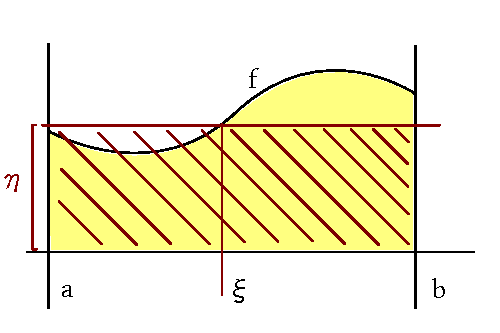
\includegraphics{img/intermediate_value_theorem.pdf}
      \caption{Intermediate value theorem where the area below the curve is given as $I = \int_a^b f(x)\, dx = \eta \cdot (b - a) = f(\xi) (b - a)$.}
    \end{center}
  \end{figure}
\end{rem}

\begin{lemma}
  Let $I = [a,b]$ and $f \in R[a,b]$ and $a \leq \alpha < \beta < \gamma \leq b$ (compare with Figure~\ref{img:nl}).
  Then $f |_{[\alpha,\gamma]} \in R[\alpha,\gamma]$.

  \begin{figure}[!h]
    \begin{center}
      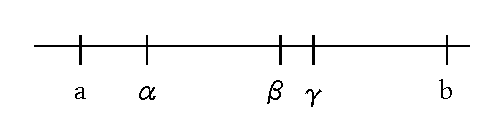
\includegraphics{img/number_line.pdf}
      \caption{Relation of $a \leq \alpha < \beta < \gamma \leq b$}
      \label{img:nl}
    \end{center}
  \end{figure}

  Furthermore it holds that
  \[ \int_{\alpha}^\beta f(x) \, dx = \int_\alpha^\beta f(x) \, dx + \int_\beta^\gamma f(x) \, dx \]
\end{lemma}

\begin{proof}
  Let $\varphi$ be a step function in $[\alpha, \gamma]$. Then $\varphi |_{[\alpha, \beta]} \in \tau[\alpha,\beta]$
  and $\varphi |_{[\beta,\gamma]} \in \tau[\beta,\gamma]$.
  Furthermore it holds (proof not given here)
  \[ \int_\alpha^\gamma \varphi \, dx = \int_\alpha^\beta \varphi \, dx = \int_\beta^\gamma \varphi \, dx \]
  For $(\varphi_n)_{n \in \mathbb N}$ a sequence of subsequences with $\varphi_n \to f$ continuous in $[\alpha,\gamma]$.
  \[ \Rightarrow \varphi_n |_{[\alpha,\beta]} \to f|_{[\alpha,\beta]} \text{ uniform in } [\alpha,\beta] \]
  analogously for $[\beta,\gamma]$.
  \[
    \int_{\alpha}^\gamma f dx
    = \lim_{n\to\infty} \int_\alpha^\gamma \varphi_n \, dx
    = \lim_{n\to\infty} \left[\int_\alpha^\beta \varphi_n \, dx + \int_\beta^\gamma \varphi_n \, dx\right]
  \] \[
    = \underbrace{\lim_{n\to\infty} \int_\alpha^\beta \varphi_n \, dx}_{=\int_\alpha^\beta f \, dx}
    + \underbrace{\lim_{n\to\infty} \int_\beta^\gamma \varphi_n \, dx}_{=\int_\beta^\gamma f \, dx}
  \]
\end{proof}

\begin{rem}
  Notation ($\alpha,\beta \in [a,b]$):
  \[ \int_\beta^\alpha f(x) \, dx = - \int_\alpha^\beta f(x) \, dx \]
  So it follows that
  \[ \int_\alpha^\alpha f(x) \, dx = - \int_\alpha^\alpha f(x) \, dx = 0 \]
  With this notation it holds that $\forall \alpha,\beta,\gamma \in I$:
  \[ \int_\alpha^\gamma f \, dx = \int_\alpha^\beta f \, dx + \int_\beta^\gamma f(x) \, dx \]
  independent of the relation of $\alpha, \beta, \gamma$ towards each other.
  For $\alpha < \beta < \gamma$ everything is fine.

  Let's also look at $\beta < \gamma < \alpha$ as an exercise.

  Then it holds that
  \[ \int_\beta^\alpha f \, dx = \int_\beta^\gamma f \, dx + \int_\gamma^\alpha f \, dx \]
  \[ - \int_\alpha^\beta f \, dx = \int_\beta^\gamma f \, dx - \int_\alpha^\gamma f \, dx \]
  \[ \Rightarrow \int_\alpha^\gamma f \, dx = \int_\alpha^\beta f \, dx + \int_\beta^\gamma f \, dx \]

  Case $\alpha = \beta$ or $\beta = \gamma$ is trivial.
\end{rem}

\index[English]{Primitive function}
\index[German]{\foreignlanguage{ngerman}{Stammfunktion}}
\index[English]{Fundamental theorem of Calculus}
\index[German]{\foreignlanguage{ngerman}{Hauptsatz der Integralrechnung}}
\begin{theorem}[Fundamental theorem of Calculus]
  Originally formulated by Isaac Barrow (1630--1677).
  Followingly popularized by Newton (1642--1727) and Leibniz (1646--1716).

  Let $f: I \to \mathbb R$ be a regulated function. $I$ is an interval and $a \in I$ is fixed.
  For $x \in I$ we define
  \[ F(x) = \int_a^x f(\xi) \, d\xi \]
  Then it holds that (two variants/characterizations)
  \begin{enumerate}
    \item $F$ is right-sided derivable and also left-sided derivable for every $x_0 \in I$
      and it holds that
      \[ F'_+(x) = f_+(x_0) = \lim_{x\to x^+_0} f(x) \qquad \text{ and } \]
      \[ F'_-(x) = f_-(x_0) = \lim_{x\to x^-_0} f(x) \]
      Especially if $f$ is continuous in $x_0$, then $F$ is differentiable in $x_0$ with
      derivative $F'(x_0) = f(x_0)$.

      We call a function with the properties of $F$ above a \emph{primitive function} of the regulated function $f$.
    \item
      Let $\Phi: I \to \mathbb R$ be an arbitrary primitive function of $f$ and
      let $a,b \in I$. Then it holds that
      \[ \int_a^b f(\xi) \, d\xi = \Phi(b) - \Phi(a) \]
  \end{enumerate}

  The first characterization claims that (informally speaking)
  the derivative for the upper limit of the integral of $f$ gives $f$.

  Let $f = \Phi'$ ($\Phi$ is our primitive function of $f$).
  The second characterization claims that the integral of a derivative of $\Phi$ gives $\Phi$.
  \[ \int_a^b \Phi' \, dx = \Phi(b) - \Phi(a) \]
\end{theorem}

\begin{proof}
  \begin{enumerate}
    \item Let $x_1, x_2 \in I$ and wlog $x_1 \leq x_2$.
      \[ \abs{F(x_1) - F(x_2)} = \abs{\int_a^{x_1} f(\xi) \, d\xi - \int_a^{x_2} f(\xi) \, d\xi} \]
      \[ = \abs{\int_a^{x_1} f(\xi) \, d\xi + \int_{x_2}^a f(\xi) \, d\xi} \]
      \[ = \abs{\int_{x_2}^{x_1} f(\xi) \, d\xi} = \abs{\int_{x_1}^{x_2} f(\xi) \, d\xi} \]
      \[ \leq \int_{x_1}^{x_2} \abs{f(\xi)} \, d\xi \leq \abs{x_2 - x_1} \cdot \norm{f}_\infty \]
      hence $F$ is Lipschitz continuous in $I$.
      So $F$ is continuous in $I$.

      One-sided limits:

      Let $\varepsilon > 0$ arbitrary and $x_0 \in I$ and $\delta$ such that $\forall x \in (x_0, x_0 + \delta)$ it holds that:
      \[ \abs{f(x) - f_+(x_0)} < \varepsilon \]
      \begin{align*}
        &\abs{\frac{F(x) - F(x_0)}{x - x_0} - f_+(x_0)} \\
        &= \frac{1}{\abs{x - x_0}} \abs{\int_a^x f(\xi) \, d\xi - \int_a^{x_0} f(\xi) \, d\xi - f_+(x_0) \cdot (x - x_0)} \\
        &= \frac{1}{\abs{x - x_0}} \abs{\int_{x_0}^x f(\xi) \, d\xi - f_+(x_0) \int_{x_0}^x 1 d\xi} \\
        &= \frac{1}{\abs{x - x_0}} \abs{\int_{x_0}^x f(\xi) \, d\xi - \int_{x_0}^x f_+(x_0) \, d\xi} \\
        &= \frac{1}{\abs{x - x_0}} \abs{\int_{x_0}^x f(\xi) - f_+(x_0) \, d\xi} \\
        &\leq \frac{1}{\abs{x - x_0}} \int_{x_0}^x \abs{f(\xi) - f_+(x_0)} \, d\xi \\
      \intertext{$\xi \in (x_0, x) \subseteq (x_0, x_0 + \delta)$}
        &< \frac{1}{\abs{x - x_0}} \cdot \varepsilon \underbrace{\int_{x_0}^x 1 \, d\xi}_{\abs{x - x_0}} \\
        &= \varepsilon \\
        &\Rightarrow F_+'(x_0) = f_+(x_0)
      \end{align*}
      Analogously $F_-'(x_0) = f_-(x_0)$.
  \end{enumerate}
\end{proof}

\meta{lecture}{14th of April 2016}{Wolfgang Ring}

\begin{theorem}[Addition: Lipschitz continuity of differentiable functions]
  Let $I = [a,b]$, $f: I \to \mathbb R$ and $f$ is continuous in $I$.
  Let $A \subseteq I$. Let $A$ be countable and $f$ is differentiable in $I \setminus A$
  and $\exists L > 0: \abs{f'(x)} \leq L \quad\forall x \in I \setminus A$.

  Then it holds that $\forall x_1, x_2 \in I$:
  \[ \abs{f(x_1) - f(x_2)} \leq L\abs{x_1 - x_2} \]
\end{theorem}
\begin{proof}
  Without loss of generality, $x_1 < x_2$. Let $\varepsilon > 0$, define
  $F_\varepsilon: I \to \mathbb R$
  \[ F_{\varepsilon}(x) = \abs{f(x) - f(x_1)} - (L + \varepsilon) (x - x_1) \]
  Show $F_\varepsilon(x_2) \leq 0$.

  Assume there is some $\varepsilon' > 0$ with $F_{\varepsilon'}(x_2) > 0$.
  It holds that
  \begin{itemize}
    \item $F_{\varepsilon'}(A) \subseteq \mathbb R$ is countable
    \item $0 = F_{\varepsilon'}(x_1) < F_{\varepsilon'}(x_2)$.
      Because $F_{\varepsilon'}$ is continuous (by Intermediate Value Theorem,
      $[0,F_{\varepsilon'}(x_2)] \subseteq F_{\varepsilon'}([x_1, x_2])$)
      and $[0, F_{\varepsilon'}(x_2)]$ contains overcountably many points,
      $F_{\varepsilon'}(A)$ is countable.
      \[ \Rightarrow \exists \gamma: 0 < \gamma < F_{\varepsilon'}(x_2) \]
      and
      \[ \gamma \in F_{\varepsilon'}([x_1, x_2] \setminus A) \]
      Let $\underbrace{F_{\varepsilon'}^{-1}(\set{y})}_{B} \cap [x_1, x_2]
      = \setdef{x \in [x_1, x_2]}{F_{\varepsilon'}(x) = y}$.

      $B$ is bounded.
      Let $c = \sup{B}$. Let $(\xi_n)_{n \in \mathbb N}$, $\xi_n \in B$ with
      $\lim_{n\to\infty} \xi_n = c$. Then it holds that $c \in [x_1, x_2]$
      and $F_{\varepsilon'}(\xi_n) = y \xRightarrow{\text{continuity of } F_{\varepsilon'}}
      \underbrace{\lim_{n\to\infty} F_{\varepsilon'}(\xi_n)}_{y} = F_{\varepsilon'}(c)$.

      Therefore $c = \max{B} = \max\set{x \in [x_1, x_2]: F_{\varepsilon'}(x) = y}$.
      Because $F_{\varepsilon'}(x_2) > y$ and $F_{\varepsilon'}(x_1) = 0 < \gamma$,
      it holds that $x_1 < c < x_2$.

      Consider $x \in (c, x_2]$ and let $\varphi(x) \coloneqq
      \frac{F_{\varepsilon'}(x) - F_{\varepsilon'}(c)}{x - c}$.
      Furthermore $F_{\varepsilon'}(x) > \gamma = F_{\varepsilon'}(c)$ for $x \in (c,x_2]$.
      Because if we define $F_{\varepsilon'}(x) < \gamma$, then (due to Intermediate Value Theorem)
      $\exists \xi \in (x, x_2)$ with $F_{\varepsilon'}(\xi) = \gamma$, so $\exists \xi \in B$
      which would be a contradiction to $c = \max{B}$.

      \begin{align*}
        \varphi(x) &= \frac{\abs{f(x) - f(x_1)} - \abs{f(c) - f(x_1)} - (L + \varepsilon')(x - x_1 - c + x_1)}{x - c} \\
          &= \frac{\abs{f(x) - f(x_1)} - \abs{f(c) - f(x_1)} - (L + \varepsilon')(x - c)}{x - c} \\
          &\overset{\text{inv. triangle ineq.}}{\leq} \frac{\abs{f(x) - f(c)}}{x - c} - (L + \varepsilon')
      \end{align*}
      Now as far as $c \not\in A$ holds, $f$ is differentiable in $c$ and it holds that $\abs{f'(c)} \leq L$,
      hence there exists an interval $(c, d)$, $d < x_2$ and $d > c$, such that
      \[ \frac{\abs{f(x) - f(c)}}{x - c} < L + \varepsilon' \]

      Because $F_{\varepsilon'}(x) > \gamma$,
      \[ \Rightarrow \varphi(x) > 0 \qquad \forall x \in (c, x_2] \]
      \[ \Rightarrow 0 < \varphi(x) \leq \abs{f(x) - f(c)}{x - c} - (L + \varepsilon') \]
      \[ \Rightarrow \abs{\frac{f(x) - f(c)}{x - c}} > L + \varepsilon' \]

      This is a contradiction to the assumption that $F_{\varepsilon'}(x_2) > 0$.
      So $F_{\varepsilon}(x_2) \leq 0 \quad \forall \varepsilon > 0$
      \[ \Rightarrow F_0(x_2) \leq 0 \Rightarrow \abs{f(x_2) - f(x_1)} \leq L - \abs{x_2 - x_1} \]
  \end{itemize}
\end{proof}

\begin{rem}
  Let $f$ be differentiable in $[a,b]$ and $\abs{f'(x)} < L \quad \forall x \in [a,b]$.
  Let $x_1, x_2 \in [a,b]$
  \[ \abs{f(x_L) - f(x_1)} = \abs{f'(\xi) \cdot (x_2 - x_1)} \leq L \abs{x_2 - x_1} \]
  by Mean Value Theorem of differential calculus.
\end{rem}

\begin{cor}
  Let $f,g: I \to \mathbb R$. $I$ as above and $f,g$ are differentiable in $I \setminus A$,
  $A$ countable and it holds that $f'(x) = g'(x) \quad \forall x \in I \setminus A$.
  There exists a constant $k$ such that
  \[ f(x) = g(x) + k \qquad \forall x \in I \]
\end{cor}
\begin{proof}
  We use the previous Theorem for
  \[ h(x) = f(x) - g(x) \]
  Then it holds that $\abs{h'(x)} = 0 = L \quad \forall x \in I \setminus A$.
  \[ \Rightarrow \abs{h(x_1) - h(x_2)} \leq 0 \cdot \abs{x_1 - x_2} \quad \forall x_1, x_2 \in I \]
  \[ \Rightarrow h(x_1) = h(x_2) \quad \forall x_1, x_2 \in I \]
  \begin{align*}
    f(x_1) - g(x_1)
      &= f(x_2) - g(x_2) \quad \forall x_1, x_2 \in I \\
      &= k \ldots \text{ constant}
  \end{align*}
  $\forall x_1 \in I$ it holds that $f(x_1) = g(x_1) + k$.
\end{proof}

\meta{lecture}{15th of April 2016}{Wolfgang Ring}

\begin{proof}[cont, 2nd part]
  We need to show: Let $f$ be a regulated function and $\Phi$ is a
  primitive function of $f$ with the following properties
  \[ \Phi'(x) = f(x) \quad \forall x \in I \text{ where f is continuous} \]
  \[ \Phi_+'(x) = \lim_{\xi\to x_+} f(x) \]
  \[ \Phi_-'(x) = \lim_{\xi\to x_-} f(x) \quad \forall x \in I \]
  Then it holds that
  \[ \int_\alpha^\beta f(x) \, dx = \Phi(\beta) - \Phi(\alpha) \]

  \begin{proof}
    For $\Phi(x) = \int_\alpha^x f(\xi) \, d\xi = F(x)$ (where $F$ is also a primitive function)
    it holds that
    \[ \int_\alpha^\beta f(\xi) \, d\xi = F(\beta) - \underbrace{F(\alpha)}_{=0} \]
    Because $\Phi$ and $F$ are both primitive functions of $f$,
    $\Phi'$ and $F'$ correspond in all continuous points,
    hence everywhere, but one countable set.

    By the uniqueness theorem, it holds that
    \[ \Phi(x) = F(x) + c \]
    \[ F(x) = \Phi(x) - c \]
    \[ \int_a^b f(\xi)\, d\xi = F(b) - F(a) = \Phi(b) - c - \Phi(a) + c = \Phi(b) - \Phi(a) \]
  \end{proof}
\end{proof}

\index[English]{Indefinite integral}
\index[German]{\foreignlanguage{ngerman}{Unbestimmtes Integral}}
\begin{rem}[Notational remark]
  Let $f$ be a regulated function. Then we denote
  \[
    \int f(x) \, dx =
    \begin{cases}
      \text{the set of all primitive function of } f & \\
      \text{an arbitrary primitive function of } f
    \end{cases}
  \]
  $\int f(x) \, dx$ is called \emph{indefinite integral}.
\end{rem}

\begin{rem}
  \[
    \int x^n \, dx = \frac{1}{n+1} x^{n+1}
    \qquad \forall n \in \mathbb R \setminus \set{-1} \forall x > 0
  \]
  If you consider all primitive functions of the indefinite integral,
  you consider a constant $c \in \mathbb R$.
  \[
    \int x^n \, dx = \frac{1}{n+1} x^{n+1} + c
    \qquad \forall n \in \mathbb R \setminus \set{-1} \forall x > 0
  \]

  Let $x > 0$: $(\ln{x})' = \frac1x$. \\
  Let $x < 0$: $(\ln{-x})' = \frac1{-x} \cdot (-1) = \frac1x$
  \[
    \int \frac 1x \, dx = \begin{cases}
      \ln(x)  & \text{ for } x > 0 \\
      \ln(-x) & \text{ for } x < 0 \\
    \end{cases}
    = \ln{\abs{x}} \qquad \text{ for } x \neq 0
  \]

  \[ \int \cos{x} \, dx = \sin{x} \]
  \[ \int \sin{x} \, dx = -\cos{x} \]
  \[ \int e^{cx} \, dx = \frac1c \cdot e^{cx} \quad (c \neq 0) \]
\end{rem}

\begin{lemma}
  Let $f_1$ and $f_2$ be regulated functions in $I = [a,b]$ and
  there exists some countable set $A$ such that
  \[ f_1(x) = f_2(x) \qquad \forall x \in I \setminus A \]
  Then it holds that
  \[
    \int f_1(x) \, dx = \int f_2(x) \, dx \text{ and } \int_a^b f_1(x) \, dx = \int_a^b f_2(x) \, dx
    \qquad \forall a,b \in I
  \]
\end{lemma}
\begin{proof}
  Let $F_1$ be a primitive function on $f_1$, $F_2$ be a primitive function of $f_2$.
  Then it holds that $F_1' = F_2'$ in $I \setminus A$.
  Due to identity theorem:
  \[ \Rightarrow F_1 = F_2 + c \Rightarrow \int f_1 \, dx = \int f_2 \, dx \]
\end{proof}

\begin{rem}
  Example of a function, which is differentiable everywhere.
  Its derivative is not a regulated function.

  Let $I = [-1,1]$ and
  \[
    f(x) = \begin{cases}
      x^2 \cdot \sin{\frac1x} & x \neq 0 \\
      0                       & x = 0
    \end{cases}
  \]
  For $x \neq 0$ it holds that
  \[ f'(x) = 2x \cos \sin{\frac1x} - \frac{x^2}{x^2} \cdot \cos{\frac1x} \]
  \[ f'(x) = 2x \sin{\frac1x} - \cos{\frac1x} \]

  \[
    f'(0)
      = \lim_{h\to0} \frac1h \left[h^2 \cdot \sin{\frac1h} - 0\right]
      = \lim_{h\to0} \underbrace{h}_{\to0} \cdot \underbrace{\sin{\frac1h}}_{\in [-1,1]}
      = 0
  \] \[
    f'(x) = \begin{cases}
      0 & \text{ for } x = 0 \\
      \underbrace{2x \sin{\frac1x} - \cos{\frac1x}}_{\text{has no one-sided limit in } x = 0} & \text{ for } x \neq 0
    \end{cases}
  \] \[
    f'_+(0) \neq \lim_{x\to 0^+} f'(x)
  \]
\end{rem}

\subsection{Integration techniques}
%
\begin{theorem}[Integration by parts (dt. \enquote{\foreignlanguage{ngerman}{partielle Integration}})]
  Let $u,v: I \to \mathbb R$ be both primitive functions of regulated functions.
  Then also $u \cdot v$ is a primitive function of a regulated function and it holds that
  \[ \int u' v \, dx = u \cdot v - \int u \cdot v' \, dx \]
  and
  \[ \int_a^b u' v \, dx = \underbrace{u(b) \cdot v(b) - u(a) \cdot v(a)}_{\eqqcolon u \cdot v |_a^b} - \int_a^b u \cdot v' \, dx \]
\end{theorem}
\begin{proof}
  $u$ is continuous and therefore a regulated function. \\
  $v$ is continuous and therefore a regulated function.

  $u'$ and $v'$ are regulated function by assumption.
  \[ \Rightarrow (u' \cdot v + u \cdot v') \in \mathcal R(I) \]
  $u \cdot v$ is differentiable in every point in which $u$ and $v$ is differentiable.
  Let $u$ be differentiable in $I \setminus A$, $v$ is differentiable in $I \setminus B$.
  \[ \Rightarrow u \cdot v \text{ is differentiable in } I \setminus \underbrace{(A \cup B)}_{\text{countable}} \]
  In $I \setminus (A \cup B)$ it holds that
  \[ (u \cdot v)'(x) = u'(x) \cdot v(x) + u(x) v'(x) \]
  Hence the function $u \cdot v$ is primitive function of the regulated function $(u' v + u v')$.
  \[ \Rightarrow \int (u' v + uv') \, dx = u \cdot v \]
  \[ \Rightarrow \int_a^b (u' v + uv') \, dx = u(b) v(b) - u(a) v(a) \]
\end{proof}

\begin{ex}
  Let $a \neq -1$ and $x > 0$.
  \[
    \int x^a \ln{x} \, dx = \begin{vmatrix}
      u' = x^a     & u = \frac1{1+a} \cdot x^{a+1} \\
      v = \ln{x}   & v' = \frac{1}{x}
    \end{vmatrix}
  \] \[
    \overset{\text{int. by parts}}{=} \frac{1}{1+a} x^{1+a} \cdot \ln{x} - \frac{1}{1+a} \int x^a \, dx
  \] \[
    = \frac{1}{1+a} x^{1+a} \ln{x} - \frac{1}{(1 + a)^2} x^{1+a}
    = \frac{1}{1+a} x^{1+a} \left[\ln{x} - \frac{1}{1 + a}\right]
  \]
\end{ex}

\begin{ex}
  \[ \int \cos^k(x) \, dx \text{ for } k = 2,3,4,\ldots \]
  \[
    \begin{vmatrix}
      u' = \cos{x} & \Rightarrow u = \sin{x} \\
      v = \cos^{k-1}(x) & v' = - (k-1) \cdot \cos^{k-2}(x) \cdot \sin(x)
    \end{vmatrix}
  \] \begin{align*}
    \int \cos^k(x) \, dx
      &= \cos^{k-1}(x) \cdot \sin(x) + \int (k-1) \cdot \cos^{k-2}(x) \cdot \underbrace{\sin^2(x)}_{1 - \cos^2(x)} \, dx \\
      &= \cos^{k-1}(x) \cdot \sin(x) + (k-1) \cdot \int \cos^{k-2}(x) \, dx - (k-1) \cdot \int \cos^k(x) \, dx
  \end{align*}
  Recognize that we have $\int \cos^k(x) \, dx$ twice in the equation (LHS and RHS, RHS with a sign).
  \[
    k \cdot \int \cos^k(x) \, dx
      = \cos^{k-1}(x) \cdot \sin(x) + (k-1) \int \cos^{k-2}(x) \, dx
  \] \[
    \int \cos^k(x) \, dx = \frac1k \cos^{k-1}(x) \sin(x) + \frac{k-1}{k} \int \cos^{k-2}(x) \, dx
  \]
  Recursion formula.

  Analogously,
  \[ \int \sin^k(x) \, dx = -\frac1k \sin^{k-1}(x) \cos(x) + \frac{k-1}{k} \int \sin^{k-2}(x) \, dx \]
  Let $c_m = \int_0^{\frac\pi2} \cos^m(x) \, dx$. Then it holds that
  \[
    c_{2n} = \frac{(2n - 1)}{2n} \cdot \frac{(2(n-1) - 1)}{2(n-1)} \cdots \frac34 \cdot \frac12 \cdot \frac\pi2
      = \left(\prod_{k=1}^n \frac{2k - 1}{2k}\right) \cdot \frac\pi2
  \] \[
    c_{2n + 1} = \left(
      \prod_{k=1}^n \frac{2k}{2k+1}
    \right)
  \]
  Proof by complete induction:
  \begin{description}
    \item[Case $n=0$]
      \[ \int_0^{\frac\pi2} \cos^{2\cdot 0} x \, dx = \int_0^{\frac\pi2} 1 \, dx = \frac\pi2 \]
      \[ \int_0^{\frac\pi2} \cos^{2\cdot 0 + 1} x \, dx = \int_0^{\frac\pi2} \cos{x} \, dx = \sin(x)|_0^{\frac\pi2} = 1 \]
      \begin{align*}
        \int_0^{\frac\pi2} \cos^{2(n+1)} \, dx
          &= \left.\frac{1}{2(n+1)} \cdot \cos^{2(n+1)-1}(x) \cdot \sin(x) \right|_0^{\frac\pi2} \\
          &+ \frac{2(n+1) - 1}{2(n+1)} \cdot \int_0^{\frac\pi2} \cos^{2n}(x) \, dx
      \end{align*} \[
        = \frac{2n+1}{2n+2} \cdot \left(\underbrace{\prod_{k=1}^n \frac{2k-1}{2k}}_{\text{induction hypothesis}}\right) \cdot \frac\pi2
        = \left(\prod_{k=1}^{n+1} \frac{2k-1}{2k}\right) \cdot \frac\pi2
      \]
  \end{description}
\end{ex}

\begin{theorem}[Wallis product]
  (John Wallis, 1616--1703)
  \[
    \frac\pi2 = \lim_{n\to\infty} w_n
    \quad \text{with} \quad
    w_n = \prod_{k=1}^n \frac{(2k)^2}{(2k-1)(2k+1)}
    = \frac{2 \cdot 2}{1 \cdot 3} \cdot \frac{4 \cdot 4}{3 \cdot 5} \cdot \frac{6 \cdot 6}{5 \cdot 7} \ldots
  \]
\end{theorem}
\begin{proof}
  \[
    \frac\pi2 \cdot \frac{c_{2n+1}}{c_{2n}}
      = \frac\pi2 \cdot \frac{\prod_{k=1}^n \frac{2k}{2k+1}}{\prod_{k=1}^n \frac{2k-1}{2k} \cdot \frac\pi2}
      = \prod_{k=1}^n \frac{(2k)^2}{(2k + 1)(2k - 1)} = w_n
  \]
  It remains to show: $\lim_{n\to\infty} \frac{c_{2n+1}}{c_{2n}} = 1$.

  In $\left[0, \frac\pi2\right]$ it holds that $0 \leq \cos{x} \leq 1$.
  \[
    \Rightarrow \int_0^{\frac\pi2} \cos^{2n}(x) \, dx
    \geq \int_0^{\frac\pi2} \cos^{2n+1}(x) \, dx
    \geq \int_0^{\frac\pi2} \cos^{2n+2}(x) \, dx
  \] \[
    c_{2n} \geq c_{2n+1} \geq c_{2n+2}
  \] \[
    1 \geq \frac{c_{2n+1}}{c_{2n}} \geq \frac{c_{2n+2}}{c_{2n}}
    = \frac{\prod_{k=1}^{n+1} \frac{2k - 1}{2k}}{\prod_{k=1}^n \frac{2k - 1}{2k}}
    = \underbrace{\frac{2n+1}{2n+2}}_{\to 1 \text{ for } n \to \infty}
  \]
  $\Rightarrow \frac{c_{2n+1}}{c_{2n}}$ converges and limit is $1$.
  \[ \lim_{n\to\infty} \frac{\pi}2 \cdot \frac{c_{2n+1}}{c_{2n}} = \frac\pi2 = \lim_{n\to\infty} w_n \]
\end{proof}

\begin{theorem}[Substitution law]
  Let $f: I \to \mathbb R$ be a regulated function with primitive function
  $F$. Furthermore $t: [\alpha, \beta] \to I$ is continuously differentiable.
  Then $F \circ t$ is a primitive function for function $(f \circ t) \cdot t'$
  and it holds that
  \[
    \int_{\alpha}^\beta f(t(x)) \cdot t'(x) \, dx
      = \int_{t(\alpha)}^{t(\beta)} f(t) \, dt
  \]
\end{theorem}

\begin{proof}
  The right-side integral is given (according to the Fundamental Theorem) by
  \[ F(t(\beta)) - F(t(\alpha)) \]
  The left-side integral is
  \[ F(t(x))' = F'(t(x)) \cdot t'(x) \]
  Or more precisely:
  \[ \frac{d}{d\,x} F(t(x)) = \frac{d}{d\,t} F(t) \cdot \frac{d\,t}{d\,x} \]
  Hence $F \circ t$ is the primitive function of the left-side integral.
  So it holds that
  \[
    \int_a^b f(t(x)) \cdot t'(x) \, dx
    = F \circ t(b) - F \circ t(a)
    = F(t(b)) - F(t(a))
  \]
\end{proof}

\begin{ex}
  \[ \int_0^1 x \sqrt{1 + x^2} \, dx = \frac12 \int_0^1 2x \sqrt{1 + x^2} \, dx \]
  \[
    \begin{vmatrix}
      t(x) = 1 + x^2    & t'(x) = 2x \\
      f(y) = \sqrt{y}   &
    \end{vmatrix}
  \] \[
    = \frac12 \int_1^2 \sqrt{x} \, dx
    = \left.\frac12 \frac{x^{\frac32}}{\frac32} \right|_1^2
    = \frac23^{\frac32} - \frac13^{\frac32}
    = \frac13 (\sqrt{8} - 1)
  \] \[
    \int_0^1 x \cdot \sqrt{1 + x^2} \, dx =
    \begin{vmatrix}
      \overbrace{y = x^2 + 1}^{\text{transform variables}}        &   \\
      \frac{dy}{dx} = 2x & \underbrace{dy = 2x \, dx}_{\text{transformation of differences}} \\
                         & x\,dx = \frac12 \, dy
    \end{vmatrix}
  \]
  Transformation of limits:
  \[ x = 0 \Leftrightarrow y = 1 \qquad x = 1 \Leftrightarrow y = 2 \]
  \[
    = \frac12 \int_1^2 \sqrt{y} \, dy
    = \left.\frac12 \frac{y^{\frac32}}{\frac32}\right|_1^2
    = \left.\frac{(x^2 + 1)^{\frac32}}{3}\right|_0^1
  \]

  Hence it is also necessary to transform the limits.
\end{ex}

\begin{ex}[Integration by parts]
  \[
    \int \ln{x} \, dx
    = \begin{vmatrix}
      v' = 1 & v = x \\
      u = \ln{x} & u' = \frac1x
    \end{vmatrix}
    = x \ln{x} - \int x \frac{1}{x} \, dx = x \ln{x} - x
  \]
\end{ex}

\index[English]{$\pi$ is irrational}
\index[German]{\foreignlanguage{ngerman}{$\pi$ is irrational}}
\begin{theorem}
  Ivan M. Niven (published in 1947, 1915--1999)

  It holds: $\pi^2$ is an irrational number. So $\pi$ is irrational.
\end{theorem}
\begin{proof}[Proof by contradiction]
  Let $\pi^2 = \frac ab \in \mathbb Q$.

  Because $\lim_{n\to\infty} \frac{a^n}{n!} = 0$ (practicals!)
  there exists $n \in \mathbb N$ such that $\pi \frac{a^n}{n!} < 1$.

  \begin{align*}
    f(x) &= \frac1{n!} x^n (1 - x)^n \\
    \intertext{is symmetrical along axis $x = \frac12$} \\
         &= \frac1{n!} \sum_{k=n}^{2n} c_k x^k \qquad \text{ with } c_k = (-1)^{k-n} \binom{n}{k-n} = \pm \binom{n}{k-n} \in \mathbb Z \\
    f^{(\mu)}(0) &= 0 \text{ for } \mu = 0,1,\ldots,n-1 \in \mathbb Z \qquad\qquad \text{ and also:} \\
    f^{(\mu)}(1) &\in \mathbb Z \text{ for } \mu = n, n+1, \ldots, 2n \\
    f^{(\mu)}(x) &= \frac1{n!} \sum_{k=0}^{2n} \underbrace{k (k-1) \ldots (k-\mu+1)}_{= \mu!} \cdot c_k \cdot x^{k-\mu} \\
    f^{(\mu)}(0) &= \frac1{n!} \mu! \left(\pm \binom{n}{\mu-n}\right) \cdot 1 \\
                 &= \frac1{n!} \mu! \frac{n!}{(\mu - n)! (n - \mu + n)!} \\
                 &= \frac{\mu!}{(\mu - n)! (2n - \mu)!} \\
                 &= \frac{(\mu-n+1) (\mu - n + 2) \ldots \mu}{1 \cdot 2 \cdot 3 \ldots (2n - \mu)} \\
                 &\in \mathbb Z
  \end{align*}
  Why does $\in \mathbb Z$ hold?
  \[ \frac{\mu!}{n!} \underbrace{\binom{n}{\mu - n}}_{\in \mathbb Z} \in \mathbb Z \qquad n \leq \mu \leq 2n \]
  \[ (n + 1) (n + 2) \ldots \nu \in \mathbb Z \]

  \[ n \leq \mu \leq 2n \]
  $f^{(\mu)}(0) \in \mathbb Z$ for $\mu \in \set{n, n+1, \ldots, 2n}$, analogously
  $f^{(\mu)}(1) \in \mathbb Z$ for $\mu \in \set{n, n+1, \ldots, 2n}$.

  \[
    F(x) = b^n \left(\pi^{2n} f(x) - \pi^{2n-2} f''(x) + \pi^{2n-4} f^{(4)} (x) + (-1)^n f^{2n}(x) \pi^0\right)
  \] \[
    F(0) \in \mathbb Z \text{ because } f^{(\mu)}(0) \in \mathbb Z \text{ for } \mu = 0,2,4,6,\ldots,2n
  \] \[
    \pi^2 = \frac ab \qquad \pi^{2n - 2l} = \frac{a^{k-l}}{b^{n-l}}
  \] \[
    b^n \cdot \pi^{2n-2l} = a^{n-l} \cdot b^l \in \mathbb Z
  \]
  Analogously for $F(1) \in \mathbb Z$.

  \begin{align*}
    &(F'(x) \cdot \sin(\pi x) - \pi F(x) \cdot \cos(\pi x))' \\
    &= F''(x) \cdot \sin(\pi x) + \pi^2 \cdot F(x) \cdot \sin{\pi x} \\
    &+ F'(x) (\cos(\pi x) - \pi \cos{\pi x}) \\
    &= (F''(x) + \pi^2 F(x)) \cdot \sin(\pi x)
  \end{align*}
  \begin{align*}
    F''(x) &= b^n \cdot (\pi^{2n} \cdot f''(x) + \pi^{2n-2} f^{(4)}(x) + \\
    &\hspace{35pt} \pi^{2n - 4} f^{(6)}(x) - \ldots + (-1)^n f^{(2n+2)}(x)) \\
    &\implies F''(x) + \pi^2 \cdot F(x)
  \end{align*}
  \begin{align*}
    F''(x) + \pi^2 \cdot F(x)
    &= b^n (
          \pi^{2n} f''(x) - \pi^{2n - 2} f^{(4)}(x) + \pi^{2n - 4} f^{(6)}(x) + \\
    &\hspace{26pt} \ldots + (-1)^n f^{(2n + 2)}(x)) \\
    &+ b^n ( \pi^{2n + 2} f(x) - \pi^{2n} f''(x) + \pi^{2n - 2} f^{(4)}(x) - \\
    &\hspace{25pt} \pi^{2n-4} f^{(6)}(x) + \ldots + (-1)^n \pi^2 \cdot f^{(2n)}(x))
  \end{align*}
  Almost all expressions cancel each other out.
  So it holds that
  \begin{align*}
    &\left(F'(x) \cdot \sin(\pi x) - \pi F(x) \cos(\pi x)\right)' \\
    &= \pi^{2n + 2} \cdot b^n \cdot f(x) \cdot \sin(\pi x) \\
    &= \frac{a^{n+1}}{b^{n+1}} \cdot b^n \cdot f(x) \cdot \sin(\pi x) \\
    &= \frac{a^{n+1}}{b} \cdot f(x) \cdot \sin(\pi x) \\
    &= \pi^2 \cdot a^n f(x) \cdot \sin(\pi x) \\
    &= \pi \left(\pi a^n f(x) \sin(\pi x)\right) \\
    I &= \pi \int_0^1 a^n f(x) \cdot \sin(\pi x) \, dx \\
    &= \left.\frac1{\pi} \cdot \left[F'(x) \cdot \sin(\pi x) - \pi \cdot F(x) \cos(\pi x)\right]\right|_0^1 \\
    &= F(1) + F(0) \in \mathbb Z
  \end{align*}
  On the other hand it holds that
  \[ f(x) = \frac{1}{n!} \underbrace{x^{n}}_{\leq 1} (\underbrace{1 - x}_{\leq 1})^n \]
  So $0 \leq f(x) \leq \frac1{n!}$. Hence,
  \[ 0 \leq a^n f(x) \cdot \sin(\pi x) \leq \frac{a^n}{n!} < \frac{1}{\pi} \]
  So $0 < I < 1 \Rightarrow I \in \mathbb Z$. This is a contradiction to our assumption that
  $I \in \mathbb Z$.
\end{proof}

\begin{rem}
  Hence $\pi$ is not rational. So there exists no linear affine function $g(x) = ax + b$
  with $a,b \in \mathbb Z$ such that $\pi$ is root of $g$.
\end{rem}

\index[English]{Algebraic numbers}
\index[German]{\foreignlanguage{ngerman}{Algebraische numbers}}
\index[English]{Transzedente Zahlen}
\index[German]{\foreignlanguage{ngerman}{Transcedental numbers}}
\begin{rem}
  We state, $\xi \in \mathbb R$ is an \emph{algebraic} number if polynomial
  \[ P(x) = a_n x^n + a_{n-1} x^{n-1} + \ldots + a_n \]
  exists with $a_i \in \mathbb Z$ for $i = 0, \ldots, n$ and $P(\xi) = 0$.

  Algebraic numbers are a generalization of rational numbers.

  $\eta \in \mathbb R$ is called \emph{transcendental}, if $\eta$ is not algebraic.
\end{rem}

\begin{rem}
  $\pi$ is transcendental.
\end{rem}

\begin{theorem}[Integration of non-compact intervals]
  \[ \int_0^\infty e^{-x} \, dx = \lim_{c\to\infty} \int_0^c e^{-x} \, dx \]
\end{theorem}
\begin{defi}[Definition of indefinite integrals]
  Let $I$ be an interval with boundary values $a$ and $b$ with
  $- \infty \leq a < b \leq \infty$.

  Let $f$ be a regulated function in $I$. Then we define
  \begin{enumerate}
    \item if $I = [a,b)$, $\int_a^b f(x) \, dx = \lim_{\beta \to b_-} \int_a^\beta f(x) \, dx$
    \item if $I = (a,b]$, $\int_a^b f(x) \, dx = \lim_{\alpha \to a_+} \int_\alpha^a f(x) \, dx$
    \item if $I = (a,b)$, we choose $c \in I$ and $\int_a^b f(x) \, dx = \lim_{\alpha\to a_+} \int_\alpha^c f(x) \, dx + \lim_{\beta \to b_-} \int_{c}^\beta f(x) \, dx$.
  \end{enumerate}
\end{defi}

\meta{lecture}{21st of April 2016}{Wolfgang Ring}

\[ f: [a,b) \to \mathbb R \qquad b \in (-\infty, \infty] \]
\[ \int_a^b f(x) \, dx = \lim_{\beta \to b_-} \int_a^b f(x) \, dx \]

\begin{ex}[Classic examples]
  \begin{enumerate}
    \item Let $s > 1$.
      \begin{align*}
        \int_1^\infty \frac{1}{x^s} \, dx
          &= \lim \int_1^\beta x^{-s} \, dx \\
          &= \left.\frac{1}{-s+1} \cdot x^{-s+1} \right|_1^\beta \\
          &= \lim_{\beta\to\infty} \frac{1}{1 - s} \cdot \frac{1}{\beta^{s-1}} - \frac{1}{1 - s}
        \intertext{$s - 1 > 0$ and $\frac{1}{1 - s} \to 1$}
          &= \frac{1}{s - 1} \qquad \text{ so indefinite integral exists}
      \end{align*}
    \item Let $s < 1$.
      \begin{align*}
        \int_0^1 x^{-s} \, dx
          &= \lim_{\alpha\to 0_+} \int_\alpha^1 x^{-s} \, dx \\
          &= \left.\lim_{\alpha\to 0_+} \frac{1}{-s+1} x^{-s+1}\right|_{\alpha}^1 \\
          &= \frac{1}{1 - s} - \underbrace{\lim_{\alpha\to 0_+} \frac{1}{1 - s} \alpha^{1 - s}}_{= 0} \\
          &= \frac{1}{1 - s}
      \end{align*}
      Compare with Figure~\ref{img:1divs}.
    \item
      \begin{align*}
        \int_0^\infty e^{-cx} \, dx
          &= \lim_{\beta\to\infty} \int_0^\beta e^{-cx} \, dx \\
          &= \left.\lim_{\beta\to\infty} \frac{1}{-c} \cdot e^{-cx} \right|_0^\beta \\
          &= \lim_{\beta\to\infty} \left(-\frac{1}{c} \cdot e^{-c\beta}\right) + \frac1{c} \\
          &= \frac{1}{c}
      \end{align*}
    \item
      \begin{align*}
        \int_{-\infty}^{\infty} \frac{1}{1 + x^2} \, dx
          &= \lim_{\alpha\to-\infty} \int_{\alpha}^0 \frac{1}{1 + x^2} \, dx + \lim_{\beta\to0} \int_0^\beta \frac{1}{1 + x^2} \, dx \\
          &= \arctan(0) - \underbrace{\lim_{\alpha\to-\infty} \arctan(\alpha)}_{-\frac\pi2} + \underbrace{\lim_{\beta\to\infty} \arctan(\beta)}_{\frac\pi2} - \arctan(0) \\
          &= - \left(-\frac\pi2\right) + \frac\pi2 \\
          &= \pi
      \end{align*}
      Compare with Figure~\ref{img:tanarctan}.
  \end{enumerate}
\end{ex}

\begin{figure}[p]
  \begin{center}
    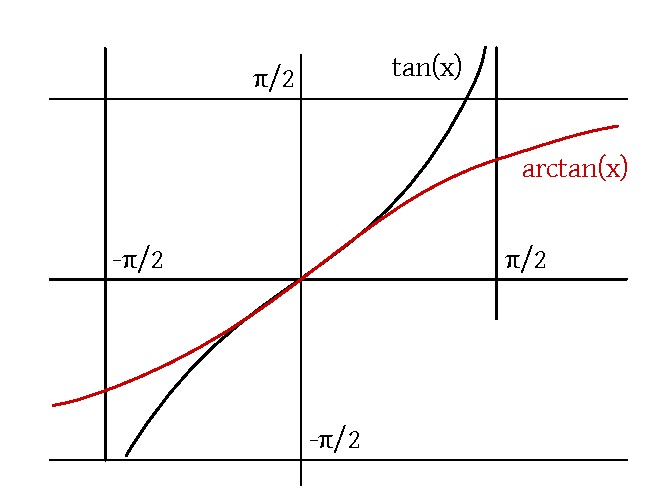
\includegraphics[width=0.3\textwidth]{img/tanarctan.pdf}
    \caption{$\tan(x)$ and $\arctan(x)$}
    \label{img:tanarctan}
    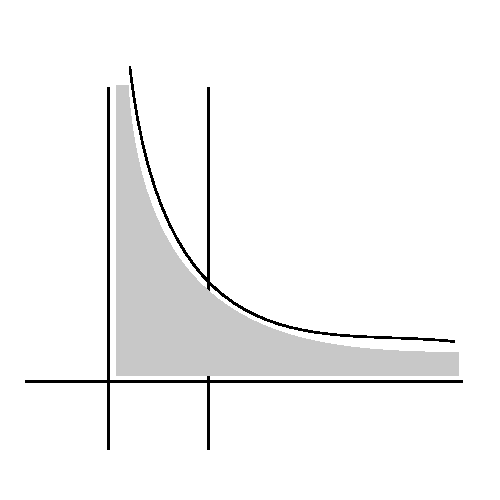
\includegraphics[width=0.2\textwidth]{img/1divsmin1.pdf}
    \caption{$\frac{1}{1 - s}$}
    \label{img:1divs}
  \end{center}
\end{figure}

\begin{rem}
  \enquote{Integral converges} means \enquote{an (indefinite) integral exists}
\end{rem}

\begin{rem}
  \[ \arctan'(x) = \frac{1}{1 + x^2} \]
  \[ \tan'(x) = \frac{\cos{x} \cdot \cos{x} - (\sin{x}) (-\sin{x})}{\cos^2{x}} = \frac{1}{\cos^2(x)} \]
  \[ \tan(x) = \frac{\sin{x}}{\cos{x}} \]
  \begin{align*}
    \arctan'(x)
      &= \frac{1}{\tan'(\arctan(x))} \\
      &= \begin{vmatrix} \arctan{x} = s \end{vmatrix} \\
      &= \left(\frac{1}{\cos^2(s)}\right)^{-1} \\
      &= \left(\frac{\cos^2(s) + \sin^2(s)}{\cos^2(s)}\right)^{-1} \\
      &= \left(1 + \left(\frac{\sin{s}}{\cos{s}}\right)^2\right)^{-1} \\
      &= \left(1 + \left[\tan(\arctan{x})\right]^2\right)^{-1} \\
      &= (1 + x^2)^{-1} \\
      &= \frac{1}{1 + x^2}
  \end{align*}
\end{rem}

\index[English]{Direct comparison test for indefinite integrals}
\index[German]{\foreignlanguage{ngerman}{Majorantenkriterium für unbestimmte Integrale}}
\begin{theorem}[Direct comparison test for indefinite integrals]
  (dt. \enquote{\foreignlanguage{ngerman}{Majorantenkriterium für uneigentliche Integrals}})
  Let $f,g$ be regulated functions in $[a,b]$ and $\abs{f(x)} \leq g(x) \quad \forall x \in [a,b)$.
  Assume $\int_a^b g(x) \, dx$ exists. Then also $\int_a^b \abs{f(x)} \, dx$ exists
  and also $\int_a^b f(x) \, dx$.
\end{theorem}

\begin{proof}
  \[ G(\beta) = \int_a^\beta g(x) \, dx \]
  We know that $\lim_{\beta\to b_-} G(\beta)$ exists.

  Cauchy criterion:
  $\forall \varepsilon > 0$ there exists a left-sided environment of $b$ such that
  for all $u,v$ in this environment it holds that
  \[ \underbrace{\abs{G(u) - G(v)}}_{\int_u^v g(x) \, dx} < \varepsilon \]
  Because $\abs{f} \leq g$ it holds that
  \[ F(\beta) = \int_a^\beta \abs{f(x)} \, dx \]
  and also that
  \[ \abs{\int_u^v \abs{f(x)} \, dx} = \abs{F(v) - F(u)} \overset{\text{monotonicity}}{\leq} \abs{\int_u^v g(x) \, dx} < \varepsilon\]
  Hence $\lim_{\beta\to b} F(\beta)$ exists because of the Cauchy criterion.
  So $\int_a^b \abs{f(x)} \, dx$ exists. Analogously for $f$ instead of $\abs{f}$.
\end{proof}

\begin{ex}
  \[ \int_0^\infty \frac{\sin{x}}{x} \, dx \text{ exists} \]
  \[
    f(x) = \begin{cases}
      \frac{\sin{x}}{x} & \text{ for } x \neq 0 \\
      1 & \text{ for } x = 0
    \end{cases}
    \text{ continuous in } 0
  \]
  \[ \int_0^1 \frac{\sin{x}}{x} \, dx = \int_0^1 f(x) \, dx \text{ exists because $f$ is continuous} \]
  \begin{align*}
    \lim_{\beta\to\infty} \int_1^\beta \frac{\sin{x}}{x} \, dx
    &= \begin{vmatrix}
      u = \frac1x & u' = -\frac1{x^2} \\
      v' = \sin{x} & v = -\cos{x}
    \end{vmatrix} \\
    &= \lim_{\beta\to\infty} \left.\frac1x \cdot (-\cos{x}) \right|_1^\beta - \int_1^\beta \frac{\cos{x}}{x^2} \, dx \\
    &= \lim_{\beta\to\infty} \left[ \underbrace{-\frac{1}{\beta} \cdot \cos{\beta}}_{\to 0} + \cos{1} - \int_1^\beta \frac{\cos{x}}{x^2} \, dx \right] \\
    &= \lim_{\beta\to\infty} \int_1^\beta \frac{\cos{x}}{x^2} \, dx
  \end{align*}
  The last expression exists, because $\frac1{x^2}$ is a majorant for $\frac{\cos(x)}{x^2}$ and $\int_1^\infty \frac{1}{x^2} \, dx$ exists.
\end{ex}

\meta{lecture}{22nd of April 2016}{Wolfgang Ring}

\[ \int_0^\infty \abs{\frac{\sin{x}}{x}} \, dx \text{ does not exist } \]
\[
  \int_{k\pi}^{(k+1)\pi} \abs{\frac{\sin{x}}{x}} \, dx
  \geq \frac{1}{(k+1) \pi} \int_{k\pi}^{(k+1)\pi} \abs{\sin{x}} \, dx
\] \[
  = \left.\frac{1}{(k+1) \pi} (\pm 1) \cdot \left(-\cos{x}\right) \right|_{k\pi}^{(k+1) \pi}
  = \frac{1}{(k+1) \pi} (\pm 1) (\pm 2)
\] \[
  = \frac{2}{(k+1)\pi}
\] \[
  \underbrace{\int_0^{(n+1)\pi} \abs{\frac{\sin{x}}{x}} \, dx}_{\text{unbounded} \Leftarrow}
    \geq \frac{2}{\pi} \cdot \underbrace{\sum_{k=0}^n \frac{1}{k+1}}_{\substack{\text{harmonic series,} \\ \text{divergent}}}
\]
In terms of the Lebesgue integral, $\int_0^\infty \frac{\sin{x}}{x} \, dx$ does not exist.

We can define new types of integration which yield new types of function which are not representable with techniques discussed so far.

\index[English]{Eulerian $\Gamma$-function}
\index[German]{\foreignlanguage{ngerman}{Eulerian $\Gamma$-function}}
\begin{ex}[The Eulerian $\Gamma$-function]
  \[ \Gamma(x) = \int_0^\infty t^{x-1} e^{-t} \, dt \text{ for } x > 0 \]
  The function variable of the $\Gamma$-function is a parameter of the integrand.
\end{ex}

The indefinite integral from above exists,
\[ \lim_{\alpha\to 0_+} \int_\alpha^1 \underbrace{t^{x-1} e^{-t}}_{>0} \, dt \text{ exists} \]
of $\int_\alpha^1 t^{x-1} e^{-t} \, dt$ is bounded in terms of $\alpha$.

\[ \int_\alpha^1 t^{x-1} \underbrace{e^{-t}}_{<1} \, dt < \underbrace{\int_\alpha^1 t^{x-1} \, dt}_{\text{converges for } x - 1 > -1} \]
hence for $x > 0$.

Right-side integral boundary:
\[ \int_1^\infty t^{x-1} e^{-t} \, dt \text{ converges?} \]

\begin{ex}[Claim]
  There exists $c > 0$ such that
  \[ t^{x-1} e^{-t} < c \cdot e^{-\frac t2} \quad \forall t \geq 1 \]

  \[ t^{x-1} \cdot e^{-\frac t2} < c \cdot e^{-\frac t2} \quad \forall t \geq 1 \]

  \begin{align*}
    \lim_{t\to\infty} \left(t^{x-1} \cdot e^{-\frac t2}\right)
    &= \begin{vmatrix} \frac t2 = s \\ t = 2s \end{vmatrix} \\
    &= \lim_{s\to\infty} (2s)^x-1 e^{-s} \\
    &\leq \lim_{s\to\infty} (2s)^{\lfloor x\rfloor + 1 - 1} \cdot e^{-s} \\
  \intertext{with $\lfloor x\rfloor \leq x < \lfloor x\rfloor + 1$}
    &= \lim_{s\to\infty} (2s)^{\lfloor x\rfloor} \cdot e^{-s} \\
    &\leq  \lim_{s\to\infty} s^{\lfloor x\rfloor + 1} \cdot e^{-s}
  \end{align*}
  because $s^{n+1} > (2s)^n$ for $s > 2^n$.

  Hence for $\varepsilon > 0$, $\exists t$ such that
  \[ \abs{t^{x-1} e^{-\frac t2}} < \varepsilon \text{ if } t > L \]
  and
  \[ \abs{t^{x-1} e^{-\frac t2}} \leq M \text{ for } t \in \underbrace{[1,L]}_{\text{compact}} \]
  $\Rightarrow$ for $t \in [1,\infty)$ it holds that
  \[
    \abs{t^{x-1} e^{-\frac t2}} \leq \max\left\{M, \varepsilon\right\} \eqqcolon c
  \]

  \[ t^{x-1} e^{-\frac t2} \leq c \]
  \[
    \int_0^\infty t^{x-1} e^{-t} \, dt
      \leq \int_0^\infty c \cdot e^{-\frac t2} \, dt
      = \left.c \cdot \left(-2 \cdot e^{-\frac t2}\right) \right|_0^\infty
      = 2c
  \]
  hence $\int_0^\infty t^{x-1} e^{-t} \, dt$ exists.

  It holds that $\Gamma(1) = 1$ because,
  \[ \int_0^\infty e^{-t} \, dt = 1 \]

  Furthermore it holds that for all $x > 0$,
  \[ \Gamma(x+1) = x \cdot \Gamma(x) \]
  \[
    \Gamma(x+1) = \int_0^\infty t^{x+1-1} e^{-t} \, dt
    = \lim_{\substack{\varepsilon \to 0 \\ R \to \infty}} \int_\varepsilon^R t^x e^{-t} \, dt
  \] \[
    = \begin{vmatrix}
      u = t^x & u' = x \cdot t^{x-1} \\
      v' = e^{-t} & v = -e^{-t}
    \end{vmatrix}
  \] \[
    = \lim_{\substack{\varepsilon \to 0 \\ R \to \infty}}\left[
      \left. -t^x e^{-t} \right|_{t=\varepsilon}^R
      + \int_\varepsilon^R x \cdot t^{x-1} \cdot e^{-t} \, dt
    \right]
  \] \[
    = \lim_{\substack{\varepsilon \to 0 \\ R \to \infty}} \left(
      \underbrace{-R^x \cdot e^{-R}}_{\to 0 \text{ for } R \to \infty} +
      \underbrace{\varepsilon^x \cdot e^{-\varepsilon}}_{\to 0 \text{ for } \varepsilon \to 0}
    \right) + x \cdot \int_0^\infty t^{x-1} e^{-t} \, dt
    = x \cdot \Gamma(x)
  \]

  So it holds that
  \begin{align*}
    T(2) &= 1 \cdot T(1) = 1 \\
    T(3) &= 2 \cdot T(2) = 2 \cdot 1 \\
    T(4) &= 4 \cdot T(3) = 3 \cdot 2 \cdot 1 \\
    T(5) &= 4 \cdot T(4) = 4 \cdot 3 \cdot 2 \cdot 1
  \end{align*}
  By complete induction we can show that
  \[ \Gamma(n+1) = n! \qquad \forall n \in \mathbb N \]
\end{ex}

\subsection{Some important inequalities}
%
\index[English]{Young's inequality}
\index[German]{\foreignlanguage{ngerman}{Young's Ungleichung}}
\begin{theorem}[Young's inequality]
  Let $f: [0, \infty) \to [0,\infty)$ be continously differentiable,
  $f(0) = 0$; $f$ is strictly monotonically increasing and unbounded
  (hence $f$ is injective because of strong monotonicity
  and surjective because of unboundedness).

  So there exists $f^{-1}: [0,\infty) \to [0,\infty)$.

  Let $a,b \geq 0$. Then it holds that
  \[ a \cdot b \leq \int_0^a f(x) \, dx + \int_0^b f^{-1}(y) \, dy \]
  Equality holds if and only if,
  \[ b = f(a) \text{ i.e. } a = f^{-1}(b) \]

  Compare with Figure~\ref{img:youngs-ineq}
\end{theorem}
\begin{figure}[!h]
  \begin{center}
    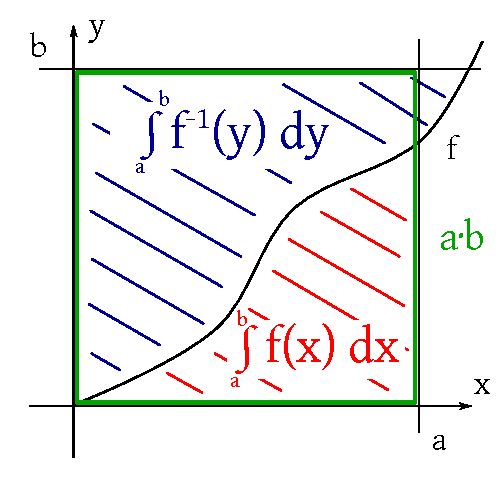
\includegraphics{img/youngs_inequality.pdf}
    \caption{Young's inequality: the blue and red areas are larger than the green area}
    \label{img:youngs-ineq}
  \end{center}
\end{figure}
\begin{proof}
  \[ \int_0^b f^{-1}(y) \, dy \overset{\text{substitution}}{=}
    \begin{vmatrix}
      y = f(x) \\
      dy = f'(x) \, dx \\
      y = 0 \Leftrightarrow x = f^{-1}(0) = 0 \\
      y = b \Leftrightarrow x = f^{-1}(b)
    \end{vmatrix}
  \]
  \begin{align*}
    &= \int_0^{f^{-1}(b)} \underbrace{f^{-1}(f(x))}_{x} \cdot f'(x) \, dx \\
    &= \int_0^{f^{-1}(b)} x \cdot f'(x) \, dx \\
    &= \left. f(x) \cdot x \right|_0^{f^{-1}(b)} - \int_0^{f^{-1}(b)} 1 \cdot f(x) \, dx \\
    &= f(f^{-1}(b)) \cdot f^{-1}(b) - \int_0^{f^{-1}(b)} f(x) \, dx \\
    &= b \cdot f^{-1}(b) - \int_0^{f^{-1}(b)} f(x) \, dx
  \end{align*}
  Therefore,
  \begin{align*}
    I
    &= \int_0^a f(x) \, dx + \int_0^b f^{-1}(y) \, dy \\
    &= \int_0^a f(x) \, dx + \int_{f^{-1}(b)}^0 f(x) \, dx + b \cdot f^{-1}(b) \\
    &= \int_{f^{-1}(b)}^a f(x) \, dx + b \cdot f^{-1}(b)
  \end{align*}

  \begin{description}
    \item[Case 1: $f^{-1}(b) = a$] ($f(a) = b$)
      \[ \implies I = \underbrace{\int_a^b f(x) \, dx}_{=0} + b \cdot a = ab \]
      Proven.
    \item[Case 2: $b < f(a) \Leftrightarrow f^{-1}(b) < a$]
      $f$ is strictly monotonically increasing, hence $f(x) > f(f^{-1}(b)) = b$
      for all $x \in (f^{-1}(b), a]$.
      \[ \int_{f^{-1}(b)}^a f(x) \, dx > b \cdot \int_{f^{-1}(b)}^a 1 \, dx \]
      \[ = b \cdot \left(a - f^{-1}(b)\right) \]
      \[ I > b \left(a - f^{-1}(b)\right) + b \cdot f^{-1}(b) = a \cdot b \]
      Proven.
    \item[Case 3: $b > f(a)$]
      \[ I = \underbrace{- \int_a^{f^{-1}(b)} f(x) \, dx}_{\text{strictly mon. decreasing}} + b f^{-1}(b) \]
      For $(-f(x))$ it holds that:
      \[ > (-f(f^{-1}(b)) = -b) \]
      \[ > (-b) \left(f^{-1}(b) - a\right) + b \cdot f^{-1}(b) = a \cdot b \]
      Proven.
  \end{description}
\end{proof}
\begin{rem}
  Young's inequality also holds if $f$ has all the properties above
  but is not necessarily differentiable.
\end{rem}
\begin{theorem}[Young's inequality, special case]
  Let $A, B \geq 0$. $p,q > 1$ such that $\frac1p + \frac1q = 1$ (hence $p$ and $q$ are \enquote{conjugate exponents}).
  Then it holds that
  \[ A \cdot B \leq \frac{A^p}{p} + \frac{B^q}{q} \]
\end{theorem}
\begin{proof}
  Let $f(x) = x^{p-1}$ satisfy the requirements for Young's inequality.
  \[ f^{-1}(y) = y^{\frac{1}{p-1}} \]
  \[ \left( \frac1q = 1 - \frac1q \qquad q = \left(1 - \frac1q\right)^{-1}\right) \]
  \[ q - 1 = \left(1 - \frac1p\right)^{-1} - 1 = \left(\frac{p-1}{p}\right)^{-1} - 1 \]
  \[ = \frac{p}{p-1} - 1 = \frac{p - p + 1}{p - 1} = \frac{1}{p-1} \]
  \[ f^{-1}(y) = y^{q-1} \]
  Therefore
  \[
    A \cdot B \leq \int_0^A x^{p-1} \, dx + \int_0^B y^{q-1} \, dy
    = \left.\frac{x^p}{p}\right|_0^A + \left.\frac{y^q}{q}\right|_0^B
    = \frac{A^p}{p} + \frac{B^q}{q}
  \]
\end{proof}
\begin{rem}
  Equality holds if $A^p = B^q$. The proof is left as an exercise to the reader.
\end{rem}

\index[English]{Hölder's inequality}
\index[German]{\foreignlanguage{ngerman}{Hölder's Ungleichung}}
\begin{theorem}[Hölder's inequality]
  Let $I$ be an interval, $a, b$ are boundary values of $I$ ($a,b \in [-\infty, \infty]$).
  Let $p,q$ be conjugate exponents, hence $p,q > 1$ and $\frac1p + \frac1q = 1$.

  Let $f_1$ and $f_2$ be regulated functions in $I$ and
  \[ \int_a^b \abs{f_1(x)}^p \, dx \text{ exists and } \int_a^b \abs{f_2(x)}^q \, dx \text{ exists} \]

  Let
  \[ \norm{f_1}_p = \left(\int_a^b \abs{f_1(x)}^p \, dx\right)^{\frac1p} \]
  and
  \[ \norm{f_2}_q = \left(\int_a^b \abs{f_2(x)}^q \, dx\right)^{\frac1q} \]
  Then it holds that
  \[
    \int_a^b \abs{f_1(x) \cdot f_2(x)} \, dx \text{ exists and }
    \int_a^b \abs{f_1(x) f_2(x)} \, dx
    \leq \norm{f_1}_p \cdot \norm{f_2}_q
  \]
\end{theorem}
\begin{proof}
  Let $A = \frac{\abs{f_1(x)}}{\norm{f_1}_p}$ and $B = \frac{\abs{f_2(x)}}{\norm{f_2}_q}$.
  \[
    A \cdot b \leq \frac{A^p}{p} + \frac{B^q}{q}
  \] \[
    \overset{\text{integration}}{\Rightarrow}
    \int_a^b \frac{\abs{f_1(x)}}{\norm{f_1}_p} \cdot \frac{\abs{f_2(x)}}{\norm{f_2}_q} \, dx
    \leq \frac1p \int_a^b \frac{\abs{f_1(x)}^p}{\norm{f_1}_p^p} \, dx
    + \frac1q \int_a^b \frac{\abs{f_2(x)}^q}{\norm{f_2}_q^q} \, dx
  \] \[
    \Rightarrow \frac{1}{\norm{f_1}_p \norm{f_2}_q} \cdot
    \int_a^b \abs{f_1(x) \cdot f_2(x)} \, dx
  \] \[
    \leq \frac{1}{p} \frac{1}{\norm{f_1}_p^p} \underbrace{\int_a^b \abs{f_1(x)}^p}_{\norm{f_1}_p^q} \, dx
    + \frac1q \frac1{\norm{f_2}_q^q} \underbrace{\int_a^b \abs{f_2(x)}^q}_{\norm{f_2}_q^q} \, dx
  \] \[
    = \frac1p + \frac1q = 1
  \] \[
    = \underbrace{\int_a^b \abs{f_1(x) \cdot f_2(x)} \, dx}_{\text{exists}}
    \leq \norm{f_1}_p \cdot \norm{f_2}_q
  \]
\end{proof}

\meta{lecture}{28th of April 2016}{Wolfgang Ring}

\begin{ex}[Special case $p = q = 2$]
  Let $p = q = 2$. $\frac12 + \frac12 = 1$ holds.
  \[
    \int_a^b \abs{f_1(x) \cdot f_2(x)} \, dx
    \leq \left(\int_a^b \abs{f_1(x)}^2 \, dx\right)^{\frac12}
    \cdot \left(\int_a^b \abs{f_2(x)}^2 \, dx\right)^{\frac12}
  \] \[
    \int_a^b \abs{f_1(x) \cdot f_2(x)} \, dx \geq \abs{\int_a^b f_1(x) \cdot f_2(x) \, dx}
  \]
  $f_1$ and $f_2$ such that $\norm{f_i}_2 < \infty$ for $i = 1,2$,
  then
  \[ \fun{f_1, f_2} = \int_a^b f_1(x) \cdot f_2(x) \, dx \]
  is a scalar (= inner) product in the vector space of functions
  with norm:
  \[
    \norm{f} = (\fun{f, f})^{\frac12} = \norm{f}_2
  \]
\end{ex}

\index[English]{Cauchy-Schwarz inequality}
\index[German]{\foreignlanguage{ngerman}{Cauchy-Schwarz Ungleichung}}
The resulting inequality is named \enquote{Cauchy-Schwarz inequality}
\[
  \abs{\fun{f_1, f_2}} \leq \norm{f_1}_2 \cdot \norm{f_2}_2
\]

\subsection{Elementwise integration of series}
%
\begin{lemma}
  Let $f_n \in R(I)$ with $I$ as interval, $f_n$ converges uniformly to $f$ in $I$.
  Then also $f$ is a regulated function and
  \[ \int_a^b f(x) \, dx = \lim_{n\to\infty} \int_a^b f_n(x) \, dx \]
\end{lemma}
\begin{proof}
  We know $f$ is a regulated function if and only if $f$ can be uniformly
  approximated using a step function.

  Let $\varepsilon > 0$ be arbitrary.
  Because $f$ is the uniform limit of $f_n$, there exists $n \in \mathbb N$
  such that $\inorm{f - f_N} < \frac\varepsilon2$. Because $f_N$ is a regulated
  function, there exists $\varphi \in \tau(I)$ with
  \[
    \inorm{f_N - \varphi} < \frac\varepsilon2 \Rightarrow
    \inorm{f - \varphi} \leq \inorm{f - f_N} + \inorm{f_N - \varphi}
    < \frac\varepsilon2 + \frac\varepsilon2 = \varepsilon
  \]
  Hence $f$ is a regulated function.
  Choose $N$ such that $\forall n \geq N$:
  \[ \inorm{f - f_n} < \frac\varepsilon{b - a} \]
  Then it holds that
  \begin{align*}
    \abs{\int_a^b f_n(x) \, dx - \int_a^b f(x) \, dx}
      &\leq \int_a^b \abs{f_n(x) - f(x)} \, dx \\
      &\leq \int_a^b \underbrace{\inorm{f_n - f}}_{< \frac\varepsilon{b - a}} \, dx \\
      &< \frac\varepsilon{b - a} \cdot (b - a) \\
      &= \varepsilon
  \end{align*}
\end{proof}

\begin{ex}[Application]
  Let $f(x) = \sum_{n=0}^\infty a_k x^k$ is a power series.
  Let $\rho_f$ be a convergence radius of $f$ and $0 < r < \rho_f$.
  Then it holds that
  \[ f_n(x) = \sum_{k=0}^n a_k x^k \text{ converges uniformly to $f$ in $[-r,r]$} \]
  \[ f_n \in R([-r,r]) \]
  \[
    \Rightarrow
    \int_{-r}^r f(x) \, dx
    = \lim_{n\to\infty} \int_{-r}^r f_n(x) \, dx
  \]
  The integral is determined by elementwise integration
  \[ \int_{-r}^r a_k x^k \, dx = \left. a_k \frac{x^{k+1}}{k+1} \right|_{-r}^r \]
  Analogously for integration over any compact interval $[a,b] \subset (-\rho_f, \rho_f)$
  i.e. for the indefinite integration. Hence,
  \[ \sum_{k=0}^\infty a_k \frac{x^{k+1}}{n+1} + c \]
  is primitive function of $f$ uniformly convergent on every interval
  $[-r,r] \subseteq (-\rho_f, \rho_f)$.
\end{ex}

\begin{ex}
  \[ F: \mathbb R \to \left(-\frac\pi2, \frac\pi2\right) \qquad F(x) = \arctan(x) \]
  \[
    F'(x) = f(x) = \frac{1}{1 + x^2}
    = \sum_{k=0}^\infty \left(-(x^2)\right)^k = \sum_{k=0}^\infty (-1)^k x^{2k}
    \qquad \forall x \in (-1, 1)
  \]

  Elementwise integration:
  \[ F(x) = \arctan(x) = \sum_{k=0}^\infty (-1)^k \frac{x^{2k+1}}{2k + 1} + c \]
  \[ \arctan(0) = 0 = c \]
  Hence,
  \[ \arctan(x) = \sum_{k=0}^\infty (-1)^k \frac{x^{2k+1}}{2k + 1} \quad \text{ in } (-1, 1) \]
  Compare with Figure~\ref{img:arctan-approx}
\end{ex}

\begin{figure}[!h]
  \begin{center}
    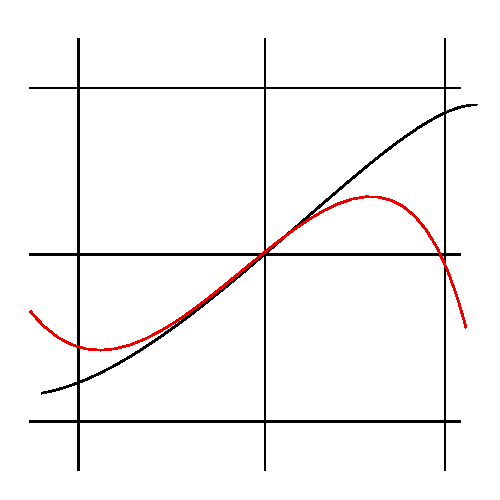
\includegraphics{img/approximation_of_arctan.pdf}
    \caption{Approximation of $\arctan(x)$}
    \label{img:arctan-approx}
  \end{center}
\end{figure}

\section{Taylor polynomials and Taylor series}
%
\begin{theorem}
  Approximation of a function with polynomials or representation
  of a function using a power series.
  \[
    \mathcal C^n((a,b))
    = \setdef{f: (a,b) \to \mathbb R}{f \text{ differentiable $n$ times in } (a,b)}
  \]
  Hence $f^{(k)}: (a,b) \to \mathbb R$ is continuous for $k = 0, 1, \ldots, n$.
  Choose $x_0 \in (a,b)$.
  Find a polynomial $T_f^a(x)$ of degree $n$ such that
  \[ \left(T_f^a\right)^{(k)}(x_0) = f^{(k)}(x_0) \]
  It holds that $T_f^a$ can be determined uniquely as
  \[ T_f^a(x) = \sum_{k=0}^n \frac{f^{(k)}(x_0)}{k!} (x - x_0)^k \]
  Taylor polynomial of $n$-th order of $f$ in point $x_0$.
\end{theorem}

\meta{lecture}{29th of April 2016}{Kniely Michael}

\begin{defi}[Additional remark to Taylor polynomials]
  Let $P(x) \coloneqq \sum_{k=0}^n a_k x^k$, $a_n \neq 0$. Let $k \in \set{1, \ldots, n}$.
  \begin{enumerate}
    \item $x_0$ is called $k$-th root of $P$ iff $P(x) = (x - x_0)^k Q(x)$ with $Q(x_0) \neq 0$.
    \item It holds that $x_0$ is a $k$-th  root of $P$ iff
      \[ \forall j \in \set{0,\ldots,k-1}: P^{(j)}(x_0) = 0 \land P^{(k)}(x_0) \neq 0 \]
  \end{enumerate}
\end{defi}
\begin{proof}[Complete induction over $k$]
  \begin{description}
    \item[$\mathbf{k=1}$] \hfill{} \\
      $\Rightarrow$: Let $x_0$ be 1st root of $P$.
        \[ P(x) = (x - x_0) Q(x) \Rightarrow P^{(0)}(x_0) = 0 \land P^{(1)}(x_0) = Q(x_0) \neq 0. \]
      $\Leftarrow$: Let $P^{(0)}(x_0) = 0$.
        \[ P^{(1)}(y_0) \neq 0 \]
        Division with remainder $\Rightarrow$
        \[ P(x) = (x - x_0) Q(x) + R(x) \text{ with } \deg(R) < \deg(x - x_0) = 1 \]
        with $R$ constant.
        \[ 0 = P(y_0) = R \Rightarrow P(x) = (x - x_0) Q(x) \]
        \[
          x \neq x_0 \Rightarrow Q(x) = \frac{P(x)}{x - x_0}
          = \frac{P(x) - P(x_0)}{x - x_0}
          \Rightarrow Q(x_0)
        \] \[
          \overset{\text{Q continuous}}{=}
          \lim_{x\to x_0} Q(x) = \lim_{x \to x_0} \frac{P(x) - P(x_0)}{x - x_0}
          = P^{(1)}(x_0) \neq 0
        \]
    \item[$\mathbf{k\geq 2, k-1 \to k}$]
      $\Rightarrow$. Let $x_0$ be the k-th root of $P$.
      Hence $P(x) = (x - x_0)^k Q(x)$ with $Q(x_0) \neq 0$.
      Let $\tilde{P}(x) \coloneqq (x - x_0)^{k-1} Q(x)$.
      $x_0$ is $(k-1)$-th root of $\tilde{P}$.
      \[
        \xRightarrow{\text{ind. hypo.}}
        \tilde{P}^{(j)}(x_0) = 0
        \land \tilde{P}^{(k-1)}(x_0) \neq 0
        \quad \forall j \in \set{0,\ldots,k-2}
      \] \[
        P(x) = (x - x_0) \tilde{P}(x) \Rightarrow
        P^{(j)}(x) = (x - x_0) \tilde{P}^{(j)}(x) + j \tilde{P}^{(j-1)}(x)
      \]
      We prove the last statement using complete induction:
      \begin{proof}
        \begin{description}
          \item[$j=0$]
            Follows immediately.
          \item[$j \geq 0, j \to j+1$]
            \[ P^{(j+1)}(x) = \left(P^{(j)}\right)'(x) \]
            \[
              = \tilde{P}^{(j)}(x) + \tilde{P}^{(j+1)}(x) (x - x_0)
            \] \[
              + j \tilde{P}^{(j)}(x)
              = (x - x_0) \tilde{P}^{(j+1)}(x) + (j+1)P^{j}(x).
            \] \[
              P^{(j)}(x_0) = j \tilde{P}^{(j-1)}(x_0)
            \] \[
              \begin{cases}
                = 0 & j = 0,\ldots,k-1 \\
                \neq 0 & j = k
              \end{cases}
            \]
        \end{description}
      \end{proof}

      We then prove the second part: $\Leftarrow$.

      Let $P^{(j)}(x_0) = 0$ for $j \in \set{0,\ldots,k-1}$, $P^{(k)}(x_0) \neq 0$.
      It holds that $P(y_0) = 0$ because of $P^{(0)}(x_0) = 0$.
      Like above: $P(x) = (x - x_0) \tilde{P}(x)$ and
      \[ P^{(j)}(x) = (x - x_0) \tilde{P}^{(j)}(x) + j \tilde{P}^{(j-1)}(x). \]
      \[ j \in \set{1,\ldots,k-1} \implies 0 = P^{(j)}(x_0) = j \cdot \tilde{P}^{(j-1)}(x_0) \]
      \[ \implies \forall l \in \set{0,\ldots,k-2}: \tilde{P}^{(l)}(x_0) = 0 \]

      \[ 0 \neq P^{(k)}(x_0) = k \tilde{P}^{(k-1)}(x_0) \Rightarrow \tilde{P}^{(k-1)}(x_0) \neq 0 \]

      induction hypothesis $\Rightarrow$
      \[ \tilde{P}(x) = (x - x_0)^{k-1} Q(x) \text{ with } Q(x_0) \neq 0 \]
      \[ \implies P(x) = (x - x_0) \tilde{P}(x) = (x - x_0)^k Q(x). \]
  \end{description}
\end{proof}

\index[English]{Taylor polynomial}
\index[German]{\foreignlanguage{ngerman}{Taylorpolynom}}
\begin{theorem}
  Let $f$ in $\mathbb C^n((a,b))$ with $n \in \mathbb N$.
  Let $a,b \in [-\infty, \infty]$, $x_0 \in (a,b)$.
  Find a polynomial $T$ of degree $n$ such property
  \begin{align}
    \forall k \in \set{0,\ldots,n}: T^{(k)}(x_0) = f^{(k)}(x_0).
    \label{taypoly}
  \end{align}
  Claim:
  \[ T_f^n(x) \equiv T_f^n(x; x_0) \coloneqq \sum_{k=0}^n \frac{f^{(k)}(x_0)}{k!} (x - x_0)^k \]
  where $x_0$ is the base point, is the only polynmial of degree $n$, which satisfies
  property~\ref{taypoly}.

  $T_f^n$ is called \emph{Taylor polynomial} of $n$-th degree of $f$ in $x_0$.
\end{theorem}
\begin{proof}
  Let $k \in \set{0,\ldots,n}$.
  \[ (T_g^n)^{(k)}(x) = \sum_{j=k}^n \frac{f^{(j)}(x_0)}{j!} j (j-1) \cdot \ldots \cdot (j - (k-1))(x - x_0)^{j-k} \]
  \[
    \left(T_f^n\right)^{(k)} (x_0)
    = \frac{f^{(k)}(x_0)}{k!} \underbrace{\left(k \cdot \ldots \cdot (k - (k-1))\right)}_{= k!}
    = f^{(k)}(x_0).
  \]
  Let $T(x) = \sum_{j=0}^n a_j x^j$ be a polynomial, which satisfies \ref{taypoly}.
  For $P \coloneqq T_g^n - T$ it holds that $P^{(k)}(x_0) = 0$ for all $k \in \set{0,\ldots,n}$.
  And $P$ is a polynomial of degree at most $n$.
  $x_0$ is at least an $(n+1)$-th root of $P \Rightarrow P \equiv 0$.
\end{proof}

\index[English]{Taylor series error}
\index[German]{\foreignlanguage{ngerman}{Taylorreihen-Fehler}}
\index[English]{Error of Taylor series}
\index[German]{\foreignlanguage{ngerman}{Fehler von Taylorreihen}}
\begin{defi}[Deviation, error, remainder]
  \[ R_g^{n+1}(x; x_0) \equiv R_g^{n+1}(x) \coloneqq f(x) - T_g^n(x; x_0) \]
\end{defi}
\begin{theorem}[Integration form of the remainder]
  Let $f \in C^{n+1}((a,b), \mathbb C)$, $n \in \mathbb N$,
  $a,b \in [-\infty, \infty], x_0, x \in (a,b)$. Then it holds that
  \[
    R_g^{n+1}(x) = \frac{1}{n!} \int_{x_0}^x (x - t)^n f^{(n+1)}(t) \, dt
  \]
\end{theorem}
\begin{proof}[Complete induction over $n$]
  Let $n = 0$.
  \[ R_g^1(x) = f(x) - T_g^0(x) = f(x) - f(x_0) \]
  \[
    \frac1{n!} \int_{x_0}^{x} (x - t)^n f^{(n+1)} (t) \, dt
    = \int_{x_0}^x f'(t) \, dt = f(x) - f(x_0).
  \]

  Consider $n\geq 1, n-1 \to n$.
  From induction hypothesis we consider
  \begin{align*}
    \Rightarrow f(x) - T_g^{n-1}(x) = R_g^n(x)
    &= \frac{1}{(n-1)!} \int_{x_0}^x (x - 1)^{n-1} f^{(n)}(t) \, dt \\
    &= - \left.\frac{(x - t)^n}{n (n-1)!} f^{(n)}(t)\right|_{x_0}^x + \int_{x_0}^x \frac{(x - t)^n}{n (n-1)!} f^{(n+1)}(t) \, dt \\
    &= \frac{(x - x_0)^n}{n!} f^{(n)}(x_0) + \frac{1}{n!} \int_{x_0}^x (x - t)^n f^{(n+1)}(t) \, dt
  \end{align*}
  \[ \Rightarrow R_f^{n+1}(x) = f(x) - T_g^n(x) = f(x) - T_g^{n-1}(x) - \frac{f^{(n)}(x_0)}{n!}(x - x_0)^n \]
  \[ = \frac{1}{n!} \int_{x_0}^x (x - t)^n f^{n+1}(t) \, dt \]

  Recognize that we consider $f$ over $\mathbb C$. In the next theorem we will only
  consider it in $\mathbb R$.
\end{proof}

\index[English]{Lagrange representation of remainder}
\index[German]{\foreignlanguage{ngerman}{Lagrange-Form des Restglieds}}
\begin{theorem}[Lagrange representation of remainder]
  Let $f \in C^{n+1}((a,b), \mathbb R), n \in \mathbb N$,
  $a,b \in [-\infty, \infty]$, $x_0,x \in (a,b)$. Then there exists some $\xi$
  between $x_0$ and $x$ such that
  \[ R_g^{n+1}(x) = \frac{f^{(n+1)}(\xi)}{(n+1)!} (x - x_0)^{n+1} \]
\end{theorem}
\begin{proof}
  \[ R_f^{n+1}(x) = \frac{1}{n!} \int_{x_0}^x (x - t)^n f^{(n+1)}(t) \, dt \]
  \begin{description}
    \item[Case 1: $x \geq x_0$:] \hfill{} \\
      \[ \forall t \in [x_0, x]: (x - t)^n \geq 0 \]
      $f \mapsto (x - 1)^n$ regulated function.
      $t \mapsto f^{(n+1)}(t)$ continuous. Hence,
      \[
        \exists \xi \in [x_0, x]:
        \int_{x_0}^x (x - 1)^n f^{n+1} (t) \, dt
        = f^{n+1}(\xi) \int_{x_0}^x (x - t)^n \, dt
      \] \[
        = f^{(n+1)}(\xi) \frac{(x - x_0)^{n+1}}{n + 1}
      \] \[
        \Rightarrow R_f^{n+1}(x) = \frac{f^{n+1}}{(n+1)!} (x - x_0)^{n+1}.
      \]
    \item[Case 2: $x < x_0$:]
      \[
        \forall t \in [x, x_0]: (t - x)^n \geq 0 \qquad \text{ analogously }
      \] \[
        \exists \xi \in [x, x_0]: \int_{x}^{x_0} (t - x)^n f^{(n+1)} (t) \, dt
      \]
      \begin{align*}
        &= f^{(n+1)}(\xi) \int_x^{x_0} (1 - x)^n \, dt \\
        &= \frac{f^{(n+1)}(\xi)}{n+1} (x_0 - x)^{n+1} \\
        &\Rightarrow R_g^{n+1}(x) = \frac{(-1)^{n+1}}{n!} \int_{x}^{x_0} (t - x)^n f^{(n+1)}(t) \, dt \\
        &= (-1)^{n+1} \frac{f^{(n+1)}(\xi)}{(n+1)!} (x_0 - x)^{n+1} \\
        &= \frac{f^{(n+1)}(\xi)}{(n+1)!} (x - x_0)^{n+1}
      \end{align*}
  \end{description}
\end{proof}

\begin{cor}[Sufficient criterion for local extremes]
  Let $f \in C^{n+1}((a,b), \mathbb R), x_0 \in (a,b)$ with
  $f^{(n)}(x_0) = \ldots = f^{(n)}(x_0) = 0, f^{(n+1)}(x_0) \neq 0$.
  Then $f$ has the following in $x_0$:
  \begin{itemize}
    \item a strict local minimum, if $n$ is odd and $f^{(n+1)}(x_0) > 0$.
    \item a strict local maximum, if $n$ is odd and $f^{(n+1)}(x_0) < 0$.
    \item no extreme, if $n$ is even.
  \end{itemize}
\end{cor}
\begin{proof}
  \begin{description}
    \item[Case 1: $f^{(n+1)}(x_0) > 0$:] \hfill{} \\
      $f^{(n+1)}$ is continuous $\Rightarrow$
      \[ \exists \varepsilon > 0: f^{(n+1)} > 0 \text{ in } (x_0 - \varepsilon, x_0 + \varepsilon) \eqqcolon I \]
      by Induction hypothesis it holds that
      \[ \forall x \in (a,b): f(x) = T_g^n(x) + R_g^{n+1}(x) = f(x_0) + R_f^{n+1}(x). \]

      If $n$ is even, then $n+1$ is odd, then
      \[ \forall x \in I \setminus \set{x_0}: \exists \xi \in I: R_f^{n+1}(x) = \frac{f^{(n+1)}(\xi)}{(n+1)!} (x - x_0)^{n+1} > 0. \]
      So,
      \[ \forall x \in I \setminus \set{x_0}: f(x) > f(x_0) \]

      If $n$ is odd, $n+1$ is even, then
      \[ \forall x \in I \setminus \set{x_0}: \exists \xi \in I: R_f^{n+1}(x) = \frac{f^{(n+1)}(\xi)}{(n+1)!} (x - x_0)^{n+1} \]
      \[
        \begin{cases}
          >0 & x > x_0 \\
          <0 & x < x_0
        \end{cases}
      \]
      $\Rightarrow$ $f$ has no extremum in $x_0$.
    \item[Case 2: $f^{(n+1)}(x_0) < 0$] follows analogously like Case~1.
  \end{description}
\end{proof}
\begin{theorem}[Qualitative Taylor formula]
  Let $f \in C^n((a,b), \mathbb C), x, x_0 \in (a,b)$.
  There exists some $r \in C((a,b), \mathbb C)$ with $r(x_0) = 0$ and
  \begin{align} f(x) = T_f^n(x) + (x - x_0)^n r(x) \label{qtf} \end{align}
\end{theorem}
\begin{proof}
  Equation~\ref{qtf} only has to be shown for $f: (a,b) \to \mathbb R$,
  because for $f: (a,b) \to \mathbb C$, $f = f_R + i f_I$ with $f_R, f_I: (a,b) \to \mathbb R$.
  Representations for $f_R$ and $f_I$ provide corresponding representations for $f$.
  Hence let $f: (a,b) \to \mathbb R$. Let $r: (a,b) \to \mathbb R$.
  \[ x \mapsto \frac{f(x) - T_f^n(x)}{(x - x_0)^n}, x \neq x_0 \text{ and } r(x_0) \coloneqq 0 \]
  We only need to show: \\
  $r$ is continuous in $x_0$, hence $\lim_{x\to x_0} r(x) = r(x_0) = 0$.
  \[
    x \in (a,b) \setminus \set{x_0} \Rightarrow
    r(x) = \frac{1}{(x - x_0)^n} \left(f(x) - T_f^{n-1}(x) - \frac{f^{(n)}}{n!} (x - x_0)^n\right)
  \] \[
    = \frac{1}{(x - x_0)^n} \left(R_g^n(x) - \frac{f^{(n)}(x_0)}{n!} (x - x_0)^n\right)
  \] \[
    = \frac{1}{(x - x_0)^n} \left(\frac{f^{(n)}(\xi)}{n!} (x - x_0)^n - \frac{f^{(n)}(x_0)}{n!} (x - x_0)^n\right)
  \] \[
    = \frac{1}{n!} \left(f^{(n)}(\xi) - f^{(n)}(x_0)\right)
  \]
  $\xi$ is between $x_0$ and $x$.
  $f^{(n)}$ is continuous and $\xi \to x_0$ for $x \to x_0$
  \[ \Rightarrow r(x) = \frac{1}{n!}(f^{(n)}(\xi) - f^{(n)}(x_0)) \overset{x \to x_0}{\to} 0 \]
\end{proof}

\meta{lecture}{3rd of May 2016}{Wolfgang Ring}

\begin{theorem}
  Assumption:
  Let $f: I \to \mathbb R$ be arbitrarily often continuously derivable.
  Hence,
  \[ T_f^n(x; x_0) \text{ exists for } \forall n \in \mathbb N \]
  Therefore we can consider a power series
  \[ T_f(x; x_0) = \sum_{k=0}^\infty \frac{f^{(k)}(x_0)}{k!} (x - x_0)^k \]
  $T_f(x; x_0)$ is called Taylor series of $f$ in $x_0$.
  Is a power sereis in $\xi = (x - x_0)$.
  Converges for $\abs{\xi} = \abs{x - x_0} < \rho(T_f)$.

  If $\rho(T_f) > 0$, it holds that $T_f(x;x_0) = f(x)$?
  \[ \lim_{n\to\infty} T_f^n(x; x_0) = T_f(x; x_0) = f(x) \text{ for } \abs{x - x_0} < \rho(T_f) \]
  is \emph{not} always satisfied.
\end{theorem}

\begin{ex}
  \[
    f(x) = \begin{cases}
      e^{-\frac1x} & \text{ for } x > 0 \\
      0 & \text{ for } x < 0
    \end{cases}
  \]
  Compare with Figure~\ref{img:e1x}.
  \begin{figure}[!h]
    \begin{center}
      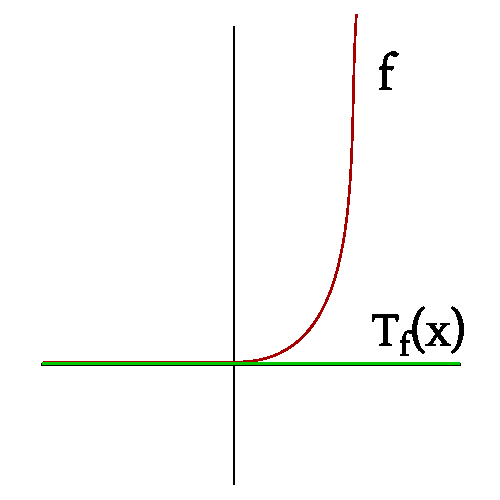
\includegraphics[width=150px]{img/e1x.pdf}
      \caption{Plot of $f$}
      \label{img:e1x}
    \end{center}
  \end{figure}
  \[ f_-^{(n)}(0) = 0 \]
  \[ f_+^{(n)}(0) = \lim_{x\to0^+} f^{(n)}(x) \]

  \[ f^{(n)}(x) = R(x) \cdot e^{-\frac1x} \]
  with $R(x) = \frac{P(x)}{Q(x)}$ with $P$ and $Q$ as polynomials.
  $R$ is a rational function (i.e. division of two polynomials).

  \[ \lim_{x\to0_+} R(x) \cdot e^{-\frac1x} = 0 \]
  Hence $f^{(n)}(0) = 0$ and therefore Taylor series
  $T_f(x; 0) = \sum_{k=0}^\infty \frac{0}{k!} x^k = 0$.
\end{ex}

\begin{rem}
  Taylor:
  \[ R_f(x) = T_f(x; 0) - f(x) \]
  It holds that
  \[ \abs{R_f(x)} \leq c_n \cdot \abs{x}^n \qquad \forall n \in \mathbb N \]
\end{rem}

\begin{theorem}
  Let $f(x) = \sum_{k=0}^\infty a_k (x - x_0)^k$ be a power series in $\xi = x - x_0$.
  Let $\rho(f) > 0$. We already know that $f$ is differentiable for all $\abs{\xi} = \abs{x - x_0} < \rho(f)$ (differentiable by $x$) and $f'$ is a power series with convergence radius $\rho(f') = \rho(f)$.
  \[ f'(x) = \sum_{k=1}^\infty a_k \cdot k x^{k-1} \]
  By complete induction it follows that:
  \begin{itemize}
    \item For all $n \in \mathbb N$ there exists $f^{(n)}(x)$ as power series of form
      \[
        f^{(n)}(x)
        = \sum_{k=n}^\infty a_k \cdot k \cdot (k-1) \cdot (k-2)
          \cdot \ldots (k-n+1) \cdot x^{k-n}
      \]
    \item
      $f^{(n)}$ as convergent power series is a continuous function. Hence,
      \[ f^{(n)}(x_0) = a_n \cdot n \cdot (n-1) \cdot (n-2) \ldots (n-n+1) = a_n \cdot n! \]
      \[ a_n = \frac{f^{(n)}(x_0)}{n!} \]
      Backsubstitution in the power series yields
      \[
        f(x) = \sum_{k=0}^\infty a_k (x - x_0)^k
          = \sum_{k=0}^\infty \frac{f^{(k)}(x_0)}{k!} (x - x_0)^k
          = T_f(x; x_0)
      \]
      Hence $f$ has a power series representation, then the power series is the Taylor series in $f$.
  \end{itemize}
\end{theorem}

\index[English]{Analytical function}
\index[German]{\foreignlanguage{ngerman}{Analytische Funktion}}
\begin{rem}
  A function representable with a power series is called \emph{analytical}.
  In the complex space, once differentiable means arbitrary often differentiable.
\end{rem}

\section{Curves in $\mathbb R^n$}
%
\index[English]{Parametric curve}
\index[German]{\foreignlanguage{ngerman}{Parametrische Kurve}}
\index[English]{Trace of a curve}
\index[German]{\foreignlanguage{ngerman}{Trace of the curve}}
\begin{defi}
  A parametric curve is a map $\gamma: I \to \mathbb R^n$ where $I$ is an interval which has form
  \[
    \gamma(t) = \begin{bmatrix}
      \gamma_1(t) \\
      \gamma_2(t) \\
      \vdots \\
      \gamma_n(t)
    \end{bmatrix}
  \]
  and every function $\gamma_i: I \to \mathbb R$ ($i = 1, \ldots, n$) is continuous.
  Often we write $\gamma_i(t) = x_i(t)$.
  If every $\gamma_i$ is differentiable in $I$, a differentiable, parametric curve
  is given. $t$ is the curve parameter.

  We call $\Gamma = \setdef{\gamma(t)}{t \in I} = \gamma(I) \subseteq \mathbb R^n$
  the \emph{trace of the curve $\gamma$}.
\end{defi}

\begin{ex}
  \[ \gamma: [0, 4\pi] \to \mathbb R^2 \]
  \[ \gamma(t) = \begin{bmatrix} \cos(t) \\ \sin(t) \end{bmatrix} \]
  In this example, every point on the curve is hit twice by the function.

  \[ \Gamma = \setdef{\begin{bmatrix} x_1 \\ x_2 \end{bmatrix} \in \mathbb R}{x_1^2 + x_2^2 - 1 =0 } \]
  $F(x_1, x_2) = x_1^2 + x_2^2 - 1 = 0$ is called trace equation of the curve
  \[ \tilde{\gamma}(t) = \begin{bmatrix} \cos{t} \\ -\sin{t} \end{bmatrix} \text{ in } I = [0, 4\pi] \]

  If $\begin{bmatrix} x_1 \\ x_2 \end{bmatrix} = \begin{bmatrix} \cos{t} \\ \sin{t} \end{bmatrix}$, then
  \[ x_2^1 + x_2^2 - 1 = \cos^2(t) + \sin^2(t) - 1 = 1 - 1 = 0 \]
  On the inverse, let $\begin{bmatrix} x_1 \\ x_2 \end{bmatrix} \in \mathbb R^2$ with $x_1^2 + x_2^2 = 1$. Then there exists $t \in [0,2\pi)$ such that $x_1 = \cos{t}$ and $x_2 = \sin{t}$.

  In this example it holds that $\tilde{\gamma} \neq \gamma$, but $T = \tilde{T}$.
\end{ex}

\begin{ex}
  Let $\tilde{\gamma}(t) = \begin{bmatrix} \cos{t} \\ \sin{t} \end{bmatrix}$ with $\tilde{\gamma}: [0,\pi] \to \mathbb R^2$.

  \[ \forall \begin{bmatrix} x_1 \\ x_2 \end{bmatrix} \in \tilde{T}: T(x_1, x_2) = x_1^2 + x_2^2 - 1 = 0 \]
  but
  \[ \tilde{T} \neq \setdef{\begin{bmatrix} x_1 \\ x_2 \end{bmatrix}}{F(x_1, x_2) = 0} \]
\end{ex}

\index[English]{Tangential vector of a curve}
\index[German]{\foreignlanguage{ngerman}{Tangential vector}}
\begin{defi}
  Let $\gamma: I \to \mathbb R^n$ be a differentiable, parametric curve.
  We define
  \[
    \dot{\gamma}(t) =
    \begin{bmatrix} \gamma'_1(t) \\ \gamma'_2(t) \\ \vdots \\ \gamma'_n(t) \end{bmatrix}
    = \begin{bmatrix} x'_1(t) \\ x'_2(t) \\ \vdots \\ x'_n(t) \end{bmatrix}
  \]
  and we call $\dot\gamma(t)$ the derivation vector of $\gamma$ in $t$.
  If $\gamma$ is considered as motion curve, then $\dot\gamma(t)$ is considered as
  speed vector of $\gamma$ in $t$.

  Consider
  \[ \dot{\gamma}(t) = \lim_{h\to 0} \frac{1}{h} \left[\gamma(t + h) - \gamma(t)\right] \]
  as illustrated in Figure~\ref{img:curve_example}.

  \begin{figure}[!h]
    \begin{center}
      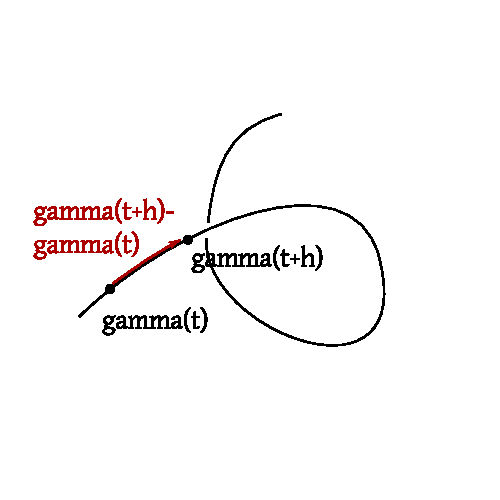
\includegraphics{img/curve_example.pdf}
      \caption{Curve example}
      \label{img:curve_example}
    \end{center}
  \end{figure}

  If $\dot{\gamma}(t) \neq 0$, then $\dot{\gamma}$ is tangential in $\Gamma$
  and we call $\dot\gamma(t)$ the \emph{tangential vector of $\gamma$ in $t$}.

  If $\dot\gamma(t) \neq 0$, we set
  \[ T_\gamma(t) = \frac{\dot\gamma(t)}{\norm{\dot\gamma(t)}_2} \]
  and we call $T_\gamma(t)$ the tangential unit vector of $\gamma$ in $t$.
\end{defi}

\begin{ex}
  \[ \gamma: \mathbb R \to \mathbb R^2 \]
  \[ \gamma(t) = \begin{bmatrix} t^2 - 1 \\ t^3 - 1 \end{bmatrix} \text{ differentiable} \]

  \[ \gamma(1) = \begin{bmatrix} 1-1 \\ 1-1 \end{bmatrix} = \vec0 \]
  \[ \gamma(-1) = \begin{bmatrix} 1-1 \\ -1+1 \end{bmatrix} = \vec0 \]

  \begin{figure}[!h]
    \begin{center}
      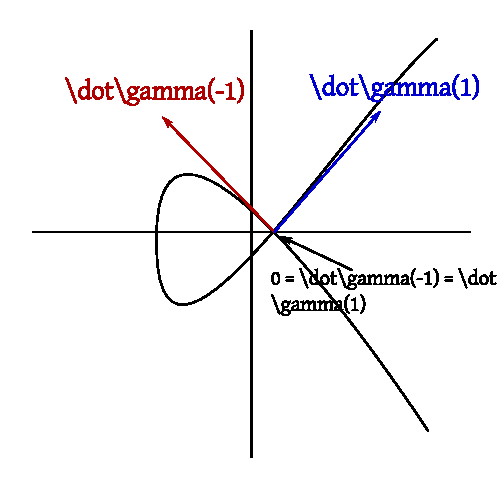
\includegraphics{img/double_point.pdf}
      \caption{A double pointed curve}
      \label{img:dbl-point}
    \end{center}
  \end{figure}

  This curve has a double point, meaning that one point is crossed two times (compare with Figure~\ref{img:dbl-point}).
  \[ \dot\gamma(t) = \begin{bmatrix} 2t \\ 3t^2 - 1 \end{bmatrix} \]
  \[ \dot\gamma(-1) = \begin{bmatrix} -2 \\ 2 \end{bmatrix} \]
  \[ \dot\gamma(1) = \begin{bmatrix} 2 \\ 2 \end{bmatrix} \]
\end{ex}

\index[English]{Regular curve}
\index[German]{\foreignlanguage{ngerman}{Reguläre Kurve}}
\begin{defi}
  Let $\gamma: I \to \mathbb R^n$ be a differentiable, parametric curve.
  $\gamma$ is called \emph{regular} curve, if $\dot\gamma(t) \neq \vec0 \quad \forall t \in I$.
\end{defi}

\index[English]{Neil's parabola}
\index[German]{\foreignlanguage{ngerman}{Neilsche Parabel}}
\begin{ex}
  \[ \gamma(t) = \begin{bmatrix} t^2 \\ t^3 \end{bmatrix} \]
  is called \emph{Neil's parabola} and non-regular.
  \[ \dot\gamma(t) = \begin{bmatrix} 2t \\ 3t^3 \end{bmatrix} \]
  \[ \dot\gamma(0) = \vec0 \]
  Has no tangent in the root.
\end{ex}

\begin{figure}[!h]
  \begin{center}
    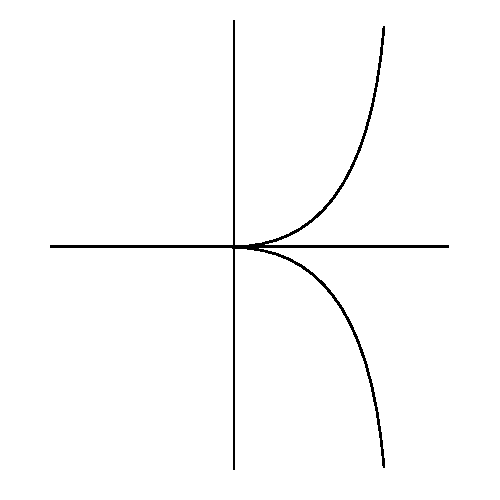
\includegraphics{img/neils_parabola.pdf}
    \caption{Neil's parabola}
  \end{center}
\end{figure}

\begin{ex}
  \[
    \gamma(t)
    = \begin{bmatrix} x_1(t) \\ x_2(t) \end{bmatrix}
    = \begin{bmatrix} a\cos(t) \\ b\sin(t) \end{bmatrix}
  \]
  $a, b > 0$ and $t \in [0,2\pi]$.
  We search for a trace equation of $\gamma$:
  \[
    \frac{x_1(t)}{a} = \cos(t)
    \qquad
    \frac{x_2(t)}{b} = \sin(t)
  \]

  We use the trace equation of the unit circle:
  \[ \left(\frac{x_1}{a}\right)^2 + \left(\frac{x_2}{b}\right)^2 - 1 = 0 \]
  \[ \frac{x_1^2}{a^2} + \frac{x_2^2}{b^2} = 1 \]

  $\gamma$ has an ellipsis as trace with major axis lengths $a$ and $b$.
  The interpretation of curve parameter $t$ is given in Figure~\ref{img:curpar}.

  \begin{figure}[!h]
    \begin{center}
      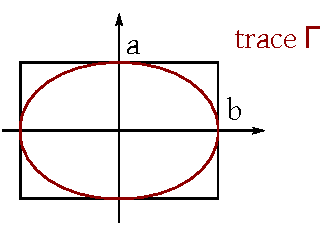
\includegraphics{img/curve_parameter.pdf}
      \caption{Curve parameter $t$}
      \label{img:curpar}
    \end{center}
  \end{figure}
\end{ex}

\meta{lecture}{6th of May 2016}{Wolfgang Ring}

\section{Hyperbolic functions}

\index[English]{Cosine hyperbolic function}
\index[German]{\foreignlanguage{ngerman}{Cosinus Hyperbolicus Funktion}}
\index[English]{Hyperbolic cosine function}
\index[English]{Sine hyperbolic function}
\index[German]{\foreignlanguage{ngerman}{Sine Hyperbolicus Funktion}}
\index[English]{Hyperbolic sine function}
\begin{defi}
  We define the \emph{cosine and sinus hyperbolic functions} as follows:
  \[ \cosh: \mathbb C \to \mathbb C \qquad \cosh(z) = \frac12 \left(e^z + e^{-z}\right) \]
  \[ \sinh: \mathbb C \to \mathbb C \qquad \sinh(z) = \frac12 \left(e^z - e^{-z}\right) \]

  For real values we get Figure~\ref{img:coshsinh}.

  Properties:
  \begin{align*}
    \cosh'(x) &= \frac12 (e^x - e^{-x}) \\
    &= \sinh(x) \\
    \sinh'(x) &= \frac12 (e^x + e^{-x}) \\
    &= \cosh(x) \\
    \cosh^2(x) - \sinh^2(x) &= \frac14 \left(e^{2x} + 2 \underbrace{e^x e^{-x}}_{=1} + e^{-2x} \right) \\
      & -\frac14 \left(e^{2x} - 2 \underbrace{e^x e^{-x}}_{=1} + e^{-2x}\right) \\
      &= \frac14 \cdot 4 \cdot 1 = 1 \\
    \cosh^2(x) - \sinh(x) &= 1
  \end{align*}
\end{defi}

\begin{figure}[!h]
  \begin{center}
    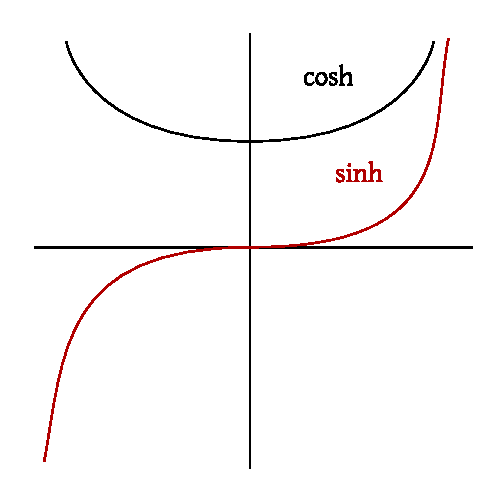
\includegraphics{img/sinhcosh.pdf}
    \caption{Plot of hyperbolic cosine and sine}
    \label{img:coshsinh}
  \end{center}
\end{figure}

\begin{ex}
  Let $y: \mathbb R \to \mathbb R^2$.
  \[
    \gamma(t)
      = \begin{bmatrix} \underbrace{a \cosh(t)}_{>0} \\ b \sinh(t) \end{bmatrix}
      = \begin{bmatrix} x(t) \\ y(t) \end{bmatrix}
  \] \[
    \frac{(x(t))^2}{a^2} - \frac{(y(t))^2}{b^2} = \cosh^2(t) - \sinh^2(t) = 1
  \]
  hence the trace $T$ of $\gamma$ is inside the hyperbola
  \[ H = \setdef{\begin{bmatrix} x \\ y \end{bmatrix} \in \mathbb R^2}{\frac{x^2}{a^2} - \frac{y^2}{b^2} = 1} \]
  \begin{figure}[h!]
    \begin{center}
      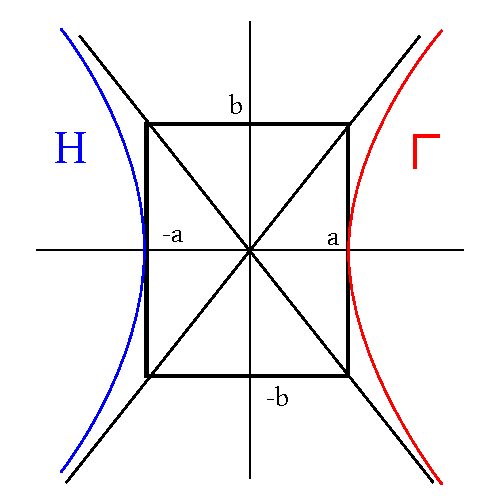
\includegraphics{img/hyperbolic_hyperbola.pdf}
      \caption{Hyperbola $H$}
    \end{center}
  \end{figure}
\end{ex}

\begin{theorem}
  Let $I \subseteq \mathbb R$ be an interval and $f: I \to \mathbb R$
  continuously differentiable. Then
  \[
    \left.\begin{array}{c}
      t \mapsto \begin{bmatrix} t \\ f(t) \end{bmatrix} \\
      I \to \mathbb R^2
    \end{array}\right\}
  \]
  a parametric, differentiable curve.
  The function graph is equivalent to the trace of the curve.
\end{theorem}

\begin{theorem}[Representation as function graph]
  Let $\gamma: I \to \mathbb R^2$ a continuously differentiable curve,
  $I$ is an interval and
  \[
    \gamma(t) = \begin{bmatrix} \gamma_1(t) \\ \gamma_2(t) \end{bmatrix}
    = \begin{bmatrix} x(t) \\ y(t) \end{bmatrix}
  \]
  it holds that
  \[ \dot{\gamma}_1(t) \neq 0 \quad \forall t \in I \]
  Then there exists a continuously differentiable function
  $f: J = \gamma_1(I) \to \mathbb R$ such that the graph of $f$
  matches the trace of $\gamma$.

  Let $x_0 = \gamma_1(t_0)$. Then it holds that
  \[ f'(x_0) = \frac{\dot{y}(t_0)}{\dot{x}(t_0)}. \]
  If $\gamma$ is differentiable twice in $t_0$,
  then $f$ is differentiable twice in $x_0$.
  \[ f''(x_0) = \frac{\dot{x}(t_0) \ddot{y}(t_0) - \ddot{x}(t_0) \dot{y}(t_0)}{[\dot{x}(t_0)]^3} \]
\end{theorem}
\begin{proof}
  $\dot{y}_1$ has no root, is continuous,
  this means $\dot{\gamma}_1$ has a uniform sign in $I$.
  Hence $\gamma_1$ is strictly monotonical in $I$.
  So $\gamma_1: I \to J = \gamma_1(I)$ is bijective.

  Let $\gamma_1^{-1}: J \to I$ be the inverse function.
  Because $\dot{\gamma}_1 \neq 0$ in $I$ is $\gamma_1^{-1}$ is differentiable
  with
  \[ \left(\gamma_1^{-1}\right)'(s) = \frac{1}{\dot{\gamma}_1(\gamma_1^{-1}(s))} \]
  We define \[ f(x) = \gamma_2(\gamma_1^{-1}(x)) \]
  \[ I \to \mathbb R \]

  Let $T_f = \setdef{(x, f(x))}{x \in I}$ be the graph of $f$ and $(x, f(x)) \in T_f$;
  $(x, f(x)) = (x, \gamma_2(\gamma_1^{-1}(x)))$.
  Let $\gamma_1^{-1}(x) = t \in I$ and therefore $x = \gamma_1(t)$. So it holds that
  \[ (x, f(x)) = (\gamma_1(t), \gamma_2(t)) \in T \qquad \text{\dots{} trace of } \gamma \]

  On the opposite, we have $(\gamma_1(t), \gamma_2(t)) \in T$.
  Let $x = \gamma_1(t) \in J$ and $t = \gamma_1^{-1}(x)$ and $(\gamma_1(t), \gamma_2(t)) = (x, \gamma_2(\gamma_1^{-1}(x))) = (x, f(x)) \in T_f$.

  \[ \left.f'(x)\right|_{x = x_0} = \dot{\gamma}_2(\gamma_1^{-1}(x_0)) \cdot \frac{1}{\dot{\gamma}_1^{-1}(x_0)} = \frac{\dot{y}(t_0)}{\dot{x}(t_0)} \]
  Let $\gamma_1^{-1}(x_0) = t_0$.

  \[
    f''(x_0) = \frac{\ddot{\gamma_2}(t_0) \cdot \frac{1}{\dot{\gamma}_1(t_0)} \cdot \dot{\gamma}_1(t_0) - \dot{\gamma}_2(t_0) \cdot \ddot{\gamma}_1(t_0) \cdot \frac{1}{\dot{\gamma}_1(t_0)}}{(\dot{\gamma}_1(t_0))^2}
  \] \[
    = \frac{\ddot{\gamma}_2(t_0) \cdot \dot{\gamma}_1(t_0) - \ddot{\gamma}_1(t_0) \cdot \dot{\gamma}_2(t_0)}{(\dot{x}(t_0))^3}
  \]
  \[ = \frac{\ddot{\gamma}(t_0) \cdot \dot{x}(t_0) - \dot{y}(t_0) \ddot{x}(t_0)}{(\dot{x}(t_0))^3} \]
\end{proof}

Figure~\ref{img:parametriccurve} gives an example for a curve which is not representable as function graph of $x$ in $\dot\gamma(t_0) = 0$.

\begin{figure}[h!]
  \begin{center}
    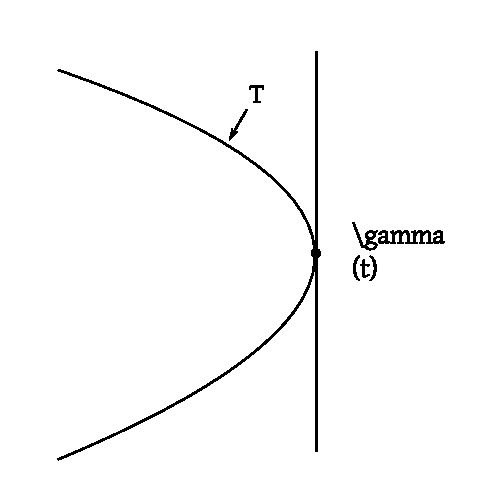
\includegraphics{img/parametric_curve_hyperbola.pdf}
    \caption{A parametric curve with $\dot\gamma(t_0) = 0$}
    \label{img:parametriccurve}
  \end{center}
\end{figure}

\section{Arc length of a parametric curve}
%
\begin{theorem}
  Let $\gamma: I = [a,b] \to \mathbb R^n$ be a parametric curve.
  Let $z = \set{t_0 = a, t_1, t_2, \ldots, t_N = b}$ with $t_{i-1} < t_i$
  for $i = 1, \ldots, N$ be a partition of the interval $I$.
  We denote the length of the polygonal line through the partition points
  $\gamma(t_0)$, $\gamma(t_1)$, \ldots, $\gamma(t_N)$ with
  \[ s(z) = s_{\gamma}(z) = \sum_{i=1}^{N} \norm{\gamma(t_1) - \gamma(t_{i-1})} \]

  Let $z^*$ be more detailed than $z$. Then it holds that
  \[ s(z^*) \geq s(z) \]
\end{theorem}
\begin{figure}[!h]
  \begin{center}
    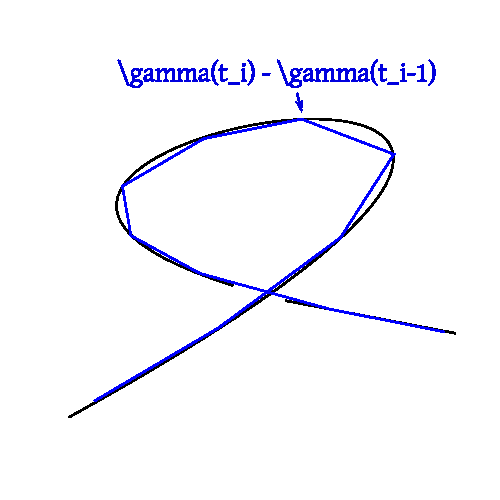
\includegraphics{img/arc.pdf}
    \caption{Approximation of the arc length}
  \end{center}
\end{figure}
\begin{proof}[Insertion of partition points]
  Let $z = \set{t_0 < t_1 < \ldots < t_N}$ and $z^* = \set{t_0 < \ldots < t_{k-1} < t' < t_k < \ldots < t_N}$.
  \begin{align*}
    s(z)   &= \sum_{i=1}^N \norm{\gamma(t_i) - \gamma(t_{i-1})} \\
    s(z^*) &= \sum_{i=1}^{k-1} \norm{\gamma(t_i) - \gamma(t_{i-1})} \\
           & + \underbrace{\norm{\gamma(t') - \gamma(t_{k-1})} + \norm{\gamma(t_k) - \gamma(t')}}_{\geq \norm{\gamma(t_K) - \gamma(t') + \gamma(t') - \gamma(t_{K-1})}} \\
           &+ \sum_{i=K+1}^N \norm{\gamma(t_i) - \gamma(t_{i-1})} \\
           &\geq \sum_{i=1}^N \norm{\gamma(t_1) - \gamma(t_{i-1})} = s(z)
  \end{align*}
  For insertion of multiple points use induction.
\end{proof}

\index[English]{Rectifiable curve}
\index[German]{\foreignlanguage{ngerman}{Rektifizierbare Kurve}}
\index[English]{Length of a curve}
\index[German]{\foreignlanguage{ngerman}{Länge einer Kurve}}
\index[English]{Curve length}
\index[German]{\foreignlanguage{ngerman}{Kurvenlänge}}
\begin{defi}
  Let $\gamma: I = [a,b] \to \mathbb R^n$ be a continuous curve.
  $\gamma$ is call \emph{rectifiable} if
  \[ s(\gamma) = \sup{s(z)} < \infty \]
  where $z$ is a partition of $I$.
  In this case $s(\gamma)$ is called length of curve $\gamma$.
\end{defi}
\begin{ex}
  Let $\gamma: I \to \mathbb R^n$ be Lipschitz continuous.
  Hence
  \[ \exists L \geq 0: \norm{\gamma(s) - \gamma(t)} \leq L(s - 1)  \]
  for all $s,t \in I$. Then $\gamma$ is rectifiable and $s(\gamma) \leq L \cdot (b-a)$.
\end{ex}
\begin{proof}
  Let $z$ be a partition of $I$.
  \[ z = \set{t_0 < t_1 < t_2 < \ldots < z_N} \]
  Then it holds that
  \begin{align*}
    s(z) &= \sum_{i=1}^N \norm{\gamma(t_i) - \gamma(t_{i-1})} \\
         &\leq \sum_{i=1}^N L \abs{t_i - t_{i-1}} \\
         &= L \sum_{i=1}^N (t_i - t_{i-1}) \\
         &= L (t_N - t_0) = L(b - a)
  \end{align*}
\end{proof}

\begin{theorem}
  Let $\gamma: I \to \mathbb R^n$ be a continuous curve.
  \[
    \gamma(t) = \begin{bmatrix}
      \gamma_1(t) \\
      \vdots \\
      \gamma_n(t)
    \end{bmatrix}
  \]
  Let every $\gamma_i: I \to \mathbb R$ be a primitive function of a regulated function
  (hence $\dot{\gamma}_i$ exists for all $t$ except for finitely many points,
  furthermore $\dot{\gamma}_i$ has left-sided and right-sided limits everywhere).
  \[ I = [a,b] \]
  Then $\gamma$ is rectifiable and it holds that
  \[ s(\gamma) = \int_a^b \norm{\dot{\gamma}(t)} \, dt \]
\end{theorem}

\begin{rem}[Some necessary preparations]
  \[
    \int_a^b \gamma(t) \, dt \coloneqq
    \begin{bmatrix}
      \int_a^b \gamma_1(t) \, dt \\
      \int_a^b \gamma_2(t) \, dt \\
      \vdots \\
      \int_a^b \gamma_n(t) \, dt
    \end{bmatrix}
  \]
\end{rem}

\begin{lemma}
  Let $\gamma: [a,b] \to \mathbb R^n$ be a continuous curve.
  Then it holds that
  \[ \norm{\int_a^b \gamma(t) \, dt} \leq \int_a^b \norm{\gamma(t)} \, dt \]
\end{lemma}
\begin{proof}
  Let $\varphi_i$ be a step function which approximates $\gamma_i$ uniformly.
  Hence, we assume that $\inorm{\varphi_i - \gamma_i} < \varepsilon$.
  $z_i$ is a partition such that $\varphi_i$ is constant at every interval.

  Define $z = \bigcup_{i=1}^n z_i$ ascendingly ordered.
  Then every $\varphi_i$ is also a step function in terms of $z$.
  \[ z = \set{t_0 < t_1 < \ldots < t_N} \]
  \[ \varphi_i(t) = c^i_k \quad \text{ for } t \in (t_{k-1}, t_k) \]
  \[ \int_a^b \varphi_i(t) \, dt = \sum_{k=1}^n c_k^i (t_k - t_{k-1}) \]
  Build
  \[
    \varphi(t) = \begin{bmatrix}
      \varphi_1(t) \\
      \vdots \\
      \varphi_N(t)
    \end{bmatrix}
  \]
  Then it holds that
  \[
    \norm{\int_a^b \varphi(t) \, dt} = \norm{
      \begin{bmatrix}
        \sum_{k=1}^N c_k^1 (t_k - t_{k-1}) \\
        \sum_{k=1}^N c_k^2 (t_k - t_{k-1}) \\
        \vdots \\
        \sum_{k=1}^N c_k^n (t_k - t_{k-1})
      \end{bmatrix}
    } = \norm{\sum_{k=1}^N (t_k - t_{k-1}) \cdot \begin{bmatrix} c_k^1 \\ \vdots \\ c_k^n \end{bmatrix}}
  \] \[
    \underbrace{\leq}_{\text{triangle ineq. in } \mathbb R^n} \sum_{k=1}^N (t_k - t_{k-1})
    \norm{\begin{bmatrix} c_k^1 \\ \vdots \\ c_k^n \end{bmatrix}}
    = \int_a^b \underbrace{\norm{\varphi(t)}}_{\text{step function in } \mathbb R} \, dt
  \] \[
    \norm{\gamma(t) - \varphi(t)} = \left(\sum_{i=1}^n \abs{\gamma_i(t) - \varphi_i(t)}^2\right)^{\frac12}
  \] \[
    \leq \left(\sum_{i=1}^n \varepsilon^2\right)^{\frac12} = \sqrt{n} \cdot \varepsilon
  \] \[
    \Rightarrow \int_a^b \norm{\gamma(t) - \varphi(t)} \, dt < \varepsilon \sqrt{n} (b - a)
   \] \[
    \norm{\int_a^b (\gamma(t) - \varphi(t)) \, dt} = \norm{
      \begin{bmatrix}
        \int_a^b \gamma_1(t) - \varphi_1(t) \, dt \\
        \int_a^b \gamma_2(t) - \varphi_2(t) \, dt \\
        \vdots \\
        \int_a^b (\gamma_n(t) - \varphi_n(t)) \, dt
      \end{bmatrix}
    }
  \] \[
    = \norm{\begin{bmatrix}
      \abs{\int_a^b (\gamma_1(t) - \varphi_1(t)) \, dt} \\
      \abs{\int_a^b (\gamma_2(t) - \varphi_2(t)) \, dt} \\
      \vdots \\
      \abs{\int_a^b (\gamma_n(t) - \varphi_n(t)) \, dt}
    \end{bmatrix}}
    \leq
    \norm{\begin{bmatrix}
      \varepsilon (b - a) \\
      \varepsilon (b - a) \\
      \vdots \\
      \varepsilon (b - a) \\
    \end{bmatrix}}
    = \varepsilon (b - a) \sqrt{n}
  \]
  Hence it holds that
  \[
    \norm{\int_a^b \gamma(t) \, dt}
    = \norm{\int_a^b \varphi(t) \, dt - \int_a^b (\varphi(t) - \gamma(t)) \, dt}
  \] \[
    \leq \norm{\int_a^b \varphi(t) \, dt} + \norm{\int_a^b (\varphi(t) - \gamma(t)) \, dt}
  \] \[
    \leq \int_a^b \norm{\varphi(t)} \, dt + \varepsilon (b - a) \sqrt{n}
  \] \[
    \leq \int_a^b \left(\norm{\varphi(t) - \gamma(t)} + \norm{\gamma(t)}\right) \, dt
    + \varepsilon (b - a) \sqrt{n}
  \] \[
    \leq \varepsilon (b - a) \sqrt{n} + \int_a^b \norm{\gamma(t)} \, dt + \varepsilon (b - a) \sqrt{n}
  \]
  Hence
  \[ \norm{\int_a^b \gamma(t) \, dt} \leq \int_a^b \norm{\gamma(t)} \, dt + 2 \varepsilon (b - a) \sqrt{n} \qquad \forall \varepsilon > 0 \]
  Hence
  \[ \norm{\int_a^b \gamma(t) \, dt} \leq \int_a^b \norm{\gamma(t)} \, dt \]
\end{proof}

\meta{lecture}{10th of May 2016}{Wolfgang Ring}

\begin{proof}[Proof of the formula for the arc length]
  Its definition depends on the parameterization.
  \[ s(\gamma) = \sup_z{s(z)} \]
  \[ s(z) = \sum_{k=1}^N \norm{\gamma(t_k) - \gamma(t_{k-1})} \]

  We show:
  \begin{enumerate}
    \item
      For all decompositions of $z$, it holds that
      \[ s(z) \leq \int_a^b \norm{\dot\gamma(t)} \, dt \]
      \[ \Rightarrow s(\gamma) \leq \int_a^b \norm{\dot\gamma(t)} \, dt \]
    \item
      \[ \forall \varepsilon > 0 \exists \text{ decomposition } z: s(\gamma) \geq s(z) \geq \int_a^b \norm{\dot\gamma(t)} \, dt - \varepsilon \]
  \end{enumerate}

  \begin{enumerate}
    \item Let $z = \set{t_0 < t_1 < \ldots < t_N}$.
      \begin{align*}
        s(z) &= \sum_{k=1}^N \norm{\gamma(t_k) - \gamma(t_{k-1})}  \\
          &\overset{\substack{\text{fundamental} \\ \text{theorem}}}{=}
            \sum_{k=1}^N \norm{\int_{t_{k-1}}^{t_k} \dot\gamma(t) \, dt} \\
          &\overset{\text{Lemma}}{=}
            \sum_{n=1}^n \int_{t_{k-1}}^{t_k} \norm{\dot\gamma(t)} \, dt \\
          &= \int_{t_0}^{t_N} \norm{\dot\gamma(t)} \, dt \\
          &= \int_a^b \norm{\dot\gamma(t)} \, dt
      \end{align*}
    \item Let $\varepsilon > 0$ be arbitrary.
      Find decomposition $z$ such that $s(\gamma) \geq s(z) \geq \int_a^b \norm{\dot\gamma(t)} \, dt - \varepsilon$.
      Let
      \[ \varphi(t) = \begin{bmatrix} \varphi_1(t) \\ \vdots \\ \varphi_n(t) \end{bmatrix} \]
      and $\varphi_t$ is a step function in $[a,b]$.

      Every $\varphi_i$ is constant in ($t_{k-1}, t_k$) for $k=1,\ldots,N$.
      and we let $z = \set{t_0, t_1, \ldots, t_N}$.
      Let $\varphi_i$ such that $\inorm{\dot\gamma_i - \varphi_i} \leq \frac{\varepsilon}{2(b - a) \sqrt{N}}$.

      Then it holds that $\forall t \in [a,b]$:
      \[ \norm{\dot\gamma(t) - \gamma(t)} = \left(\sum_{i=1}^n \abs{\dot\gamma_i(t) - \varphi_i(t)}\right)^{\frac12} \]
      \[
        \leq \left(\sum_{i=1}^n \inorm{\dot\gamma_i - \varphi_i}^2\right)^{\frac12}
        \leq \left(\sum_{i=1}^n \left(\frac{\varepsilon}{2(b - a)}^2 \cdot \frac1n\right)\right)^[\frac12]
        = \frac{\varepsilon}{2 (b - a)}
      \]
      We let
      \begin{align*}
        \inorm{\dot\gamma - \varphi}
          &= \sup\set{\norm{\dot\gamma(t) - \varphi(t)}_2: t \in [a,b]} \\
          &= \max\set{\norm{\dot\gamma(t) - \varphi(t)}_2: t \in [a,b]}
      \end{align*}
      It holds that
      \[ \inorm{\dot\gamma - \varphi} < \frac{\varepsilon}{2 (b - a)} \]
      \[ z = \set{t_0, t_1, \ldots, t_N} \]
      \[
        \norm{\int_{t_{k-1}}^{t_k} \dot\gamma(t) \, dt}
        = \norm{\int_{t_{k-1}}^{t_k} (\dot\gamma(t) - \varphi(t)) \, dt + \int_{t_{k-1}}^{t_k} \varphi(t) \, dt}
      \] \[
        \geq \norm{\int_{t_{k-1}}^{t_k} \varphi(t) \, dt} - \norm{\int_{t_{k-1}}^{t_k} (\dot\gamma(t) - \varphi(t)) \, dt}
      \]
      $\varphi$ is constant and the right summand is $\leq \int_{t_{k-1}}^{t_k} \norm{\dot\gamma(t) - \varphi(t)} \, dt$.
      \[
        \geq \int_{t_{k-1}}^{t_k} \norm{\varphi(t)} \, dt - \int_{t_{k-1}}^{t_k} \underbrace{\norm{\dot\gamma(t) - \varphi(t)}}_{< \frac{\varepsilon}{2(b-1)}} \, dt
      \] \[
        > \int_{t_{k-1}}^{t_k} \norm{\varphi(t)} \, dt - \frac{\varepsilon}{2(b - a)} (t_k - t_{k-1})
      \] \[
        s(z) = \sum_{k=1}^N \norm{\int_{t_{k-1}}^{t_k} \dot\gamma(t) \, dt}
          > \sum_{k=1}^N \int_{t_{k-1}}^{t_k} \norm{\varphi(t)} - \frac{\varepsilon}{2(b - a)} (t_{k} - t_{k-1})
      \] \[
        = \int_a^b \norm{\varphi(t)} \, dt - \frac{\varepsilon}{2(b - a)} \underbrace{(t_N - t_0)}_{= b - a}
      \] \[
        = \int_a^b \norm{\varphi(t)} \, dt - \frac{\varepsilon}{2}
      \]

      \[
        \int_a^b \norm{\varphi(t)} \, dt = \int_a^b \norm{\varphi(t) - \dot\gamma(t) + \dot\gamma(t)} \, dt
      \] \[
        \geq \int_a^b \left(\norm{\dot\gamma(t)} - \underbrace{\norm{\varphi(t) - \dot\gamma(t)}}_{< \frac{\varepsilon}{2(b - a)}}\right) \, dt
      \] \[
        = \int_a^b \norm{\dot\gamma(t)} \, dt - \frac{\varepsilon}{2}
      \] \[
        \Rightarrow s(z) > \int_a^b \norm{\dot\gamma(t)} \, dt - \frac\varepsilon2 - \frac\varepsilon2
      \] \[
        \Rightarrow s(\gamma) \geq s(z) > \int_a^b \norm{\dot\gamma(t)} \, dt - \varepsilon
        \qquad \forall \varepsilon > 0
      \] \[
        \Rightarrow s(\gamma) \geq \int_a^b \norm{\dot\gamma(t)} \, dt
      \]
  \end{enumerate}
\end{proof}

\begin{ex}[Circumference of a circle with radius $r$]
  \[
    \gamma_r(t) = r \begin{bmatrix}
      \cos(t) \\
      \sin(t)
    \end{bmatrix}
    \qquad t \in [0, 2\pi];
    \dot\gamma_t(t) = r \begin{bmatrix}
      -\sin(t) \\
      \cos(t)
    \end{bmatrix}
  \] \[
    s(\gamma_r) = \int_0^{2\pi} \norm{r \begin{bmatrix} - \sin(t) \\ \cos(t) \end{bmatrix}} \, dt
    = \int_0^{2\pi} r \, dt = 2\pi r
  \]
\end{ex}

\index[English]{Elliptic integral}
\index[German]{\foreignlanguage{ngerman}{Elliptisches Integral}}
\begin{ex}[Ellipsis]
  \[
    \gamma(t) = \begin{bmatrix}
      a \cos(t) \\
      b \sin(t)
    \end{bmatrix} \qquad a,b > 0
  \] \[
    \dot\gamma(t) = \begin{bmatrix}
      -a \sin(t) \\
      b \cos(t)
    \end{bmatrix}
  \] \[
    \norm{\dot\gamma(t)} = (a^2 \underbrace{\sin^2(t)}_{1 - \cos^2(t)} + b^2 \cos^2 (t))^{\frac12}
  \]
  Let $a \geq b$, $\varepsilon^2 = 1 - \frac{b^2}{a^2}$.
  \begin{align*}
    \norm{\dot\gamma(t)} &= (a^2 - (a^2 - b^2) \cos^2(t))^{\frac12} \\
      &= a \left(1 - \left(1 - \frac{b^2}{a^2}\right) \cos^2(t)\right)^2 \\
      &= a \left(1 - \varepsilon^2 \cos^2(t)\right)^{\frac12}
  \end{align*}
  \[ s(\gamma) = a \int_0^{2\pi} \sqrt{1 - \varepsilon^2 \cos^2(t)} \, dt \]
  This defines a new set of functions which cannot be solved with means we discussed so far.
  They are called \emph{elliptic integral}.
\end{ex}

\subsection{Change of parameters, reparameterization}
\index[English]{Reparameterization}
\index[German]{\foreignlanguage{ngerman}{Reparametrisierung}}
%
Let $\sigma: I \to J$ as smooth (ie. differentiable) as required.
$\sigma$ is bijective and $\sigma^{-1}: J \to I$ is be part
of the same differentiation class like $\sigma$.
Let $\gamma: I \to \mathbb R^n$ be a curve. We call
$\beta = \gamma \circ \sigma^{-1}: I \to \mathbb R^n$ a reparameterization
of $\gamma$ using $\sigma$. Compare with Figure~\ref{img:reparam}.

\begin{figure}[!h]
  \begin{center}
    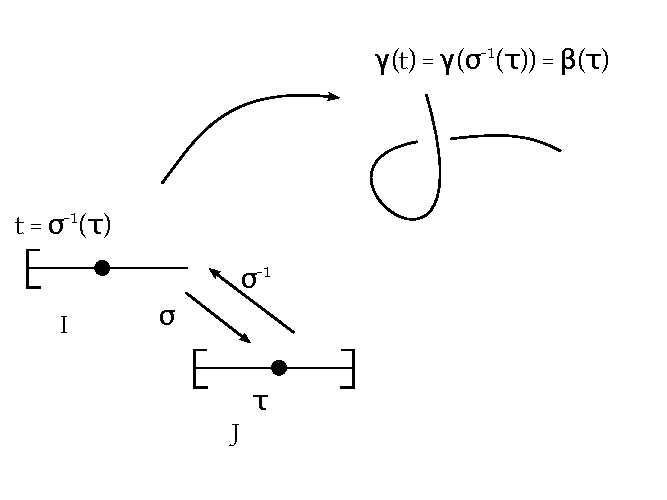
\includegraphics{img/reparameterization.pdf}
    \caption{Reparameterization: $\beta$ and $\gamma$ have the same trace}
    \label{img:reparam}
  \end{center}
\end{figure}

\index[English]{Orientation preserving reparameterization}
\index[German]{\foreignlanguage{ngerman}{Orientierungserhaltende Reparameterisierung}}
$\sigma$ is called parameter transformation.
$\gamma$ is called orientation preserving, if $\sigma$ is strictly monotonically increasing.

\index[English]{Geometric curve measures}
\index[German]{\foreignlanguage{ngerman}{Geometrisches Maß}}
A measure, defined by the curve (arc length, tangential vector, curvature, \dots)
is called \emph{geometric}, if reparameterization can be applied without modifications.

$s(\gamma)$ is obviously a geometric measure, because
\begin{enumerate}
  \item By definition of polygonal lines
  \item Let $\beta(\tau) = \gamma \circ \sigma^{-1}(\tau)$.
    \[ \dot{\beta}(\tau) = \dot{\gamma}(\sigma^{-1}(\tau)) \circ (\sigma^{-1})'(\tau) \]
    \[ \norm{\dot\beta(\tau)} = \norm{\dot\gamma(\sigma^{-1})(\tau)} \cdot \abs{(\sigma^{-1})'(\tau)} \]
    \begin{description}
      \item[Case $\sigma$ is orientation preserving]
        If and only if $\sigma' > 0 \Leftrightarrow (\sigma^{-1})' > 0$

        Let $I = [a,b]; J = [c,d]; c = \sigma(a); d = \sigma(b)$.
        \[ s(\beta) = \int_c^d \norm{\dot\gamma(\underbrace{\sigma^{-1}(\tau)}_{= t})} \cdot \underbrace{(\sigma^{-1})' (\tau) \, d\tau}_{dt} \]
        \[ = \int_a^b \norm{\dot\gamma(t)} \, dt = s(\gamma) \qquad \text{ (by substitution)} \]
      \item[Case $\sigma$ is orientation inversing]
        \[ \gamma' < 0 \qquad (\gamma^{-1})' < 0 \]
        \[ \abs{(\sigma^{-1})'(\tau)} = -(\sigma^{-1})'(\tau) \qquad \sigma(a) = d, \sigma(b) = c \]
        \[
          \int_c^d \norm{\dot\beta(\tau)} \, d\tau
          = \int_c^d \norm{\dot\gamma(\underbrace{\sigma^{-1}(\tau)}_{t})} \cdot \underbrace{\left(- (\sigma^{-1})'(\tau)\right)\, d\tau}_{dt}
        \] \[
          \begin{vmatrix}
            \tau = c \Leftrightarrow t = b \\
            \tau = a \Leftrightarrow t=  a
          \end{vmatrix}
        \] \[
          = -\int_b^a \norm{\dot\gamma(t)} \, dt
        \] \[
          = \int_a^b \norm{\dot\gamma(t)} \, dt = s(\gamma)
        \]
    \end{description}
\end{enumerate}

\subsection{Reparameterization by arc length}
%
We consider a regular curve $\gamma$, hence $\norm{\dot\gamma(t)} > 0 \quad \forall t \in I$
and let $s: I \to J = S(I)$ by
\[ s(t) = \int_a^t \norm{\dot\gamma(\tau)} \, d\tau \]

$s(t)$ is the length of the curve $\gamma$ between $a$ and $t$. Let $s(a) = 0$.
It holds that $\dot{s}(t) = \norm{\dot\gamma(t)} > 0$ (by the Fundamental Theorem of Differential and Integration Theory), hence $s$ is strictily monotonically increasing.
We use $s$ for reparameterization.
\[ \beta(\xi) = \gamma \circ s^{-1}(\xi) \]
is a reparameterization of $\gamma$ by the arc length.

\begin{align*}
  \norm{\dot\beta(\xi)}
    &= \norm{\dot\gamma(s^{-1}(\xi)) \circ (s^{-1})'(\xi)} \\
    &= \norm{\dot\gamma(s^{-1}(\xi)) \frac{1}{\dot{s}(s^{-1}(\xi))}} \\
    &= \norm{\dot\gamma(s^{-1})(\xi)} \cdot \abs{\frac{1}{\dot{s} (s^{-1}(\xi))}} \\
    &= \frac{\norm{\dot{\gamma}(s^{-1}(\xi))}}{\norm{\dot\gamma(s^{-1}(\xi))}} = 1
\end{align*}
Hence the tangential vector is the unit vector (in every point)
\[ s_{\beta}(\xi) = \int_0^{\xi} \underbrace{\norm{\dot\beta(\eta)}}_{=1} \, d\eta = \xi \]
So the curve parameter corresponds to the arc length.
On the opposite: Let $\gamma: I \to \mathbb R^n$ with property $\norm{\dot\gamma(t)} = 1 \quad\forall t \in I = [0,b]$.
Then it holds that
\[ s(t) = \int_0^t \underbrace{\norm{\dot\gamma(\tau)}}_{=1} \, d\tau = t \]
So it holds that $s = s^{-1} = \operatorname{id}_{[0,b]}$.
So $\gamma$ is parameterized by the arc length.

\begin{rem}[Notation]
  We don't write $\xi = s(t)$, but $s = s(t)$.
\end{rem}

Reparameterization by the arc length:
\[ \beta(s) = \gamma(s^{-1}(s)) = \gamma(t) \]

\meta{lecture}{12th of May 2016}{Wolfgang Ring}

\subsection{Invariance of arc length}
%
Let $\gamma: I \to \mathbb R$ be a parametric curve.
\[ \sigma: I \to J \text{ orientation-preserving parameter transformation} \]
\[ S_\gamma(t) = \int_a^t \norm{\dot\gamma(\xi)} \, d\xi \]
\[ I = [a,b] \qquad J = [c,d] \]

\[ \tilde{\gamma} = \gamma \circ \sigma^{-1}: J \to \mathbb R^n \quad \text{ reparameterization} \]
\[ S_{\tilde{\gamma}}(\tau) = \int_C^\tau \abs{\dot{\tilde{\gamma}}(\eta)} \, d\eta \]
We know that $S_{\tilde{\gamma}}(\tau) = S_{\tilde{\gamma}}(\sigma(t)) = S_{\gamma}(t)$.
\[ S_{\tilde{\gamma}} \circ \sigma = S_{\gamma} \]
Let $S = S_{\gamma}(t)$ and $\beta$ is a reparameterization of $\gamma$ by its arc length.
Hence $\beta(s) = \gamma(s^{-1}_\gamma(s))$ and $\beta = \gamma \circ S_{\gamma}^{-1}$.

\[ \tilde{\beta}(s) = \tilde{\gamma} \circ S_{\tilde{\gamma}}^{-1} = \gamma \circ \sigma^{-1} \circ \sigma \circ S_{\gamma}^{-1} = \gamma \circ S_{\gamma}^{-1} = \beta(s) \]

Hence, reparametric curves $\gamma$ and $\tilde{\gamma}$ have the same reparameterization by its arc length $\beta$.

We require orientation preservation (compare with Figure~\ref{img:arclength}).
%
\begin{figure}[!h]
  \begin{center}
    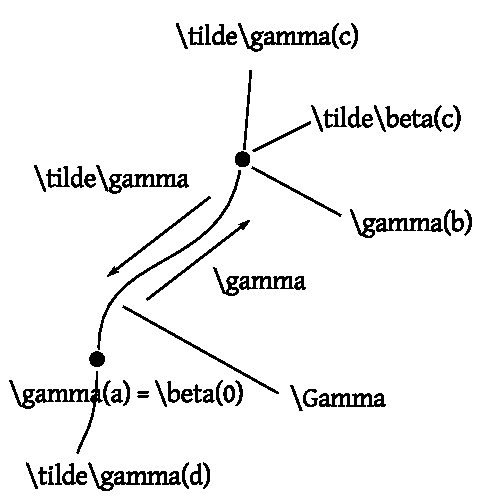
\includegraphics{img/arc_length_invariance.pdf}
    \caption{Invariance of arc length}
    \label{img:arclength}
  \end{center}
\end{figure}

Then it holds that
\[ \tilde{\beta}(s) = \beta(s(\gamma) - s) \]

Consider special case $\gamma: I \to \mathbb R^2$.

\[
  \gamma(t) = \begin{bmatrix} x(t) \\ y(t) \end{bmatrix};
  \qquad
  S_\gamma(t) = \int_a^t \sqrt{\dot{x}(\xi)^2 + \dot{y}(\xi)^2} \, d\xi
\]
or even more special:
\[ \gamma(t) = \begin{bmatrix} t \\ f(t) \end{bmatrix} \qquad \text{ \dots function graph} \]
\[ S_\gamma(t) = S_f(t) = \int_a^t \sqrt{1 + (f'(\xi))^2} \, d\xi \]


\subsection{Curvature}
%
Curvature corresponds to the rate of change of the direction of motion.
This corresponds to the rate of change of
\[ T(t) = \frac{\dot{\gamma}(t)}{\abs{\gamma(t)}} \]
in regards of the arc length.

\begin{enumerate}
  \item Let $\gamma: I \to \mathbb R^2$ be a parameterized regular curve.
    $\beta(s)$ is the reparameterization of $\gamma$ by its arc length.
    $\beta: [0, s(\gamma)] \to \mathbb R^2$.
    \[ \dot\beta(s) = T(s) \quad \text{ is a unit vector} \]
    It holds that $\langle \dot\beta(s), \dot\beta(s)\rangle = 1$,
    hence $\dot\beta_1^2(s) + \dot\beta_2^2(s) = 1$.
    $\beta$ can be differentiated twice.

    So we derive $\dot\beta_1^2(s) + \dot\beta_2^2(s)$:
    \[ 2\dot\beta_1(s) \cdot \ddot{\beta_1}(s) + 2 \dot\beta_2(s) \cdot \ddot{\beta}_2(s) = 0 \]
    So it holds with
    \[
      \ddot{\beta}(s) = \begin{bmatrix} \ddot{\beta}_1(s) \\ \ddot{\beta}_2(s) \end{bmatrix}
      \qquad
      \langle \dot{\beta}(s), \ddot{\beta}(s) \rangle = 0
    \]
    $\ddot{\beta}$ is orthogonal to $\dot{\beta} = T$.
    We define $N = \begin{bmatrix} -\dot{\beta}_2 \\ \dot{\beta}_1 \end{bmatrix} = \begin{bmatrix} 0 & -1 \\ 1 & 0 \end{bmatrix} \cdot T$.
\end{enumerate}

\begin{defi}
  We define a \emph{signed} curvature $\kappa$ in $\gamma$ in point $\gamma(t) = \beta(s)$
  by its relation
  \[ \frac{d^2 \beta}{ds^2} = \ddot{\beta}(s) = \kappa(S) \cdot N(S) \]
  $\kappa$ (with this property) actually exists, because $\ddot{\beta}$ is orthogonal to $T$
  and therefore a multiple of $N$.

  In case of reparameterization $\gamma(t) = \tilde{\gamma}(\tau)$, the arc length stays
  the same. Therefore the curvature in $\gamma(t)$ and $\dot{\gamma}(\tau)$ is also the same.
  Hence the curvature is invariant in terms of orientation-preserving reparameterization.
\end{defi}

\meta{lecture}{13th of May 2016}{Wolfgang Ring}

From now on: We denote the derivative by arc length of a function $f(s)$ using \enquote{$f'(s)$}.

Again:
\[ T'(s) = \kappa(S) \cdot N(S) \]
\[ \langle T'(s), N(s)\rangle = \kappa(S) \cdot \underbrace{\langle N(S), N(S)\rangle}_{=1} \]
\[ \kappa(S) = \langle T'(s), N(s)\rangle \]

\index[English]{Curvature radius}
\index[German]{\foreignlanguage{ngerman}{Krümmungsradius}}
\begin{ex}
  \[ \gamma(t) = r \begin{bmatrix} \cos(t) \\ \sin(t) \end{bmatrix} \]
  where $r$ is the radius. It holds that $\norm{\dot{\gamma}(t)} = r$.
  \[
    S_{\gamma}(t) = \int_0^t r \, d\xi = r \cdot t
    \implies t = \frac{s}{r}
    \implies \beta(s) = r \begin{bmatrix} \cos{\frac{s}{r}} \\ \sin{\frac{s}{r}} \end{bmatrix}
  \] \[
    \beta'(s) = r \cdot \frac1{r} \begin{bmatrix}
      -\sin{\frac{s}{r}} \\
      \cos{\frac{s}{r}}
    \end{bmatrix}
    = \begin{bmatrix}
      -\sin{\frac{s}{r}} \\
      \cos{\frac{s}{r}}
    \end{bmatrix}
    = T(s)
  \] \[
    T'(s) = \frac1r \begin{bmatrix}
      -\cos{\frac{s}{r}} \\
      -\sin{\frac{s}{r}}
    \end{bmatrix}
  \] \[
    N(s) = \begin{bmatrix}
      - \cos(\frac{s}{r}) \\
      - \sin(\frac{s}{r})
    \end{bmatrix} = D \cdot T(s)
  \] \[
    \kappa(s) = \langle T'(s), N(s)\rangle
    = \frac{1}{r} \cdot 1
    = \frac{1}{r}
  \]
  For an arbitrary curve $\gamma$ we define the \emph{curvature radius} in
  point $\gamma(t) = \beta(s)$ as $\rho(s) = \frac{1}{\kappa(s)}$
  for $\kappa(s) \neq 0$.
  $\rho(s) = \infty$ if $\kappa(s) = 0$.
\end{ex}

\begin{rem}
  Hence the curvature radius of the circle line is $r$.
  $\gamma^-(t)$ goes in counter-clockwise direction along the circumference of the circle.
  If $\gamma^-(t) = r \cdot \begin{bmatrix} \cos(t) \\ -\sin(t) \end{bmatrix}$,
  an analogous calculation can be made:
  $\kappa_{\gamma^{-}}(s) = -\frac{1}{r}$.
\end{rem}

\begin{theorem}
  Let $\gamma: I \to \mathbb R^2$ be a regular, twice continuously differentiable
  curve. Then it holds that
  \[ \kappa(t) = \kappa_{\beta}(s) = \frac{\dot{x}(t) \ddot{y}(t) - \ddot{x}(t) \dot{y}(t)}{(\dot{x}(t)^2 + \dot{y}(t)^2)^{\frac32}} \]
  if $\gamma(t) = \begin{bmatrix} t \\ f(t) \end{bmatrix}$ (function graph) it holds that
  \[ \kappa(t) = \frac{f''(t)}{(1 + f'(t)^2)^{\frac32}} \]
\end{theorem}

\begin{proof}
  \[ \beta(s) = \gamma(\underbrace{t(s)}_{s_\gamma^{-1}(s)}) \]
  \[
    \beta'(s) =
    \dot{\gamma}(t(s)) \cdot \underbrace{t'(s)}_{\frac{1}{\dot{s}_{\gamma}(s_\gamma^{-1}(s))}}
    = \dot{\gamma}(t(s)) \cdot \frac{1}{\norm{\dot{\gamma}(t(s))}}
    = \frac{1}{\dot{s}_\gamma(t(s))} \cdot \dot{\gamma}(t(s))
  \]
  Let $\frac1{\lambda} = -\frac{1}{(\dot{s}_\gamma(t(s)))^2} \cdot \ddot{s}_\gamma(t(s)) \cdot t'(s) \cdot \dot{\gamma}(t(s))$.
  \[
    \beta''(s) = -\frac{1}{(\dot{s}_\gamma(t(s)))^2} \cdot \ddot{s}_\gamma(t(s)) \cdot t'(s)
    + \frac{1}{s'_\gamma(t(s))} \cdot \ddot{\gamma}(t(s)) \cdot \underbrace{\frac{1}{\dot{s}_\gamma(t(s))}}_{t'(s)}
  \] \[
    \kappa(t) = \kappa(s(t)) = \ang{N}{T'} = \langle D\beta'(s), \beta''(s)\rangle
  \] \[
    = \ang{D \cdot \frac{1}{\dot{s}_\gamma} \dot\gamma(t(s))}{\frac{1}{\dot{s}_\gamma(t(s))^2} \cdot \ddot{\gamma}(t(s)) - \lambda \dot{\gamma}(t(s))}
  \]
  where
  \[
    \ang{D \cdot \frac{1}{\dot{s}_\gamma} \dot\gamma(t(s))}{\ddot{\gamma}(t(s)) - \lambda \dot{\gamma}(t(s))} = 0
  \]
  \[ = \underbrace{\frac{1}{(\dot{s}_\gamma(t))^3}}_{*}
  \ang{\begin{bmatrix} -\dot{y}(t) \\ \dot{x}(t) \end{bmatrix}}%
      {\begin{bmatrix} \ddot{x}(t) \\ \ddot{y}(t) \end{bmatrix}} \]
  \[ * = \norm{\dot\gamma(t)} = \sqrt{\dot{x}^2(t) + \dot{y}^2(t)} \]
  \[
    \implies
    \kappa(t) = \frac{\dot{x}(t) \ddot(t) - \dot\gamma(t) \dot{x}(t)}{(\dot{x}^2(t) + \dot{\gamma}^2(t))^{\frac32}}
  \]
\end{proof}

\index[English]{Curvature center}
\index[German]{\foreignlanguage{ngerman}{Krümmungsmittelpunkt}}
\begin{defi}
  Let $\gamma: I \to \mathbb R^2$ be a regular, twice continuously differentiable curve.
  Let $\rho(t) = \frac{1}{\kappa(t)}$ be the curvature radius in $\gamma(t)$.

  Then let
  \[ \underbrace{m(t)}_{\mathbb R^2} = \gamma(t) + \rho(t) \cdot N(t) \]
  and denote $m(t)$ as \emph{curvature center} of $\gamma$ in $\gamma(t)$
  (compare with Figure~\ref{img:curvature-center}).
\end{defi}

\index[English]{Osculating circle}
\index[German]{\foreignlanguage{ngerman}{Schmiegkreis}}
\begin{figure}[!h]
  \begin{center}
    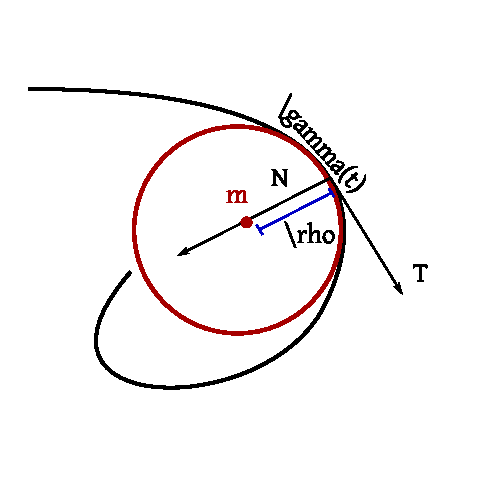
\includegraphics{img/curvature_center.pdf}
    \caption{Curvature center $m$.
      A circle with center $m$ and radius $\rho$ is called curvature radius
      or \enquote{osculating circle} (dt. \enquote{Schmiegkreis}) of $\gamma$ in $\gamma(t)$.
    }
    \label{img:curvature-center}
  \end{center}
\end{figure}

\begin{rem}
  The error (deviation) from the osculating circle is of order $\mathcal O^2$.
\end{rem}
\index[English]{Evolute}
\index[German]{\foreignlanguage{ngerman}{Evolute}}
\begin{rem}
  The curve of curvature centers $t \to m(t)$ is called \emph{evolute}
  of $\gamma$.
\end{rem}

\subsection{Situation in $\mathbb R^3$}
%
Let $\gamma: I \to \mathbb R^3$ be parameterized by its arc length.
It is twice continuously differentiable.
\[ T(s) = \beta'(s) \qquad \text{\dots tangential vector} \]
Analogously to $\mathbb R^2$ it holds that $\ang{T'(s)}{T(s)} = 0$
(this follows from $\ang{T(s)}{T(s)} = 1$).
Hence the unit vector $N(s) \coloneqq \frac{T'(s)}{\norm{T'(s)}}$
is normal to $T(s)$ (only for $T'(s) \neq 0$) and we let $\kappa(s) = \norm{T'(s)} \geq 0$.
Also it holds that $\kappa(s) N(s) = T'(s)$ and $\ang{T'(s)}{N(s)} = \kappa(s)$.

\subsection{Analysis in $\mathbb R^n$}
%
We look at some important inequalities:
%
\begin{theorem}[Jensen's inequality]
  Let $I$ be an interval, $f: I \to \mathbb R$ is convex.
  \[ \lambda_1, \lambda_2, \ldots, \lambda_n \in [0,1] \text{ and } \sum_{k=1}^{n} \lambda_k = 1 \]
  Let $x_1, \ldots, x_n \in I$. Then it holds that
  \[ f(\lambda_1 x_1 + \ldots + \lambda_n x_n) \leq \lambda_1 f(x_1) + \ldots + \lambda_n f(x_n) \]
\end{theorem}
\begin{proof}
  By complete induction over $n$:
  \begin{description}
    \item[Case $n=1$:] Trivial
    \item[Case $n=2$:] convexity
    \item[Case $n\to n+1$:] left as an exercise to the reader
  \end{description}
\end{proof}
\begin{rem}
  Reminder: $f$ is convex if
  \[
    \forall x_1, x_2 \in I, \lambda \in [0,1]:
    f(\lambda x_1 + (1 - \lambda) x_2) \leq \lambda f(x_1) + (1  - \lambda) f(x_2)
  \]
\end{rem}
\begin{rem}
  Is $f$ strictly convex, then equality holds only for $x_1 = x_2 = \ldots = x_n = x$.
\end{rem}

\begin{theorem}
  Inequality between the weighted geometric and the weighted arithmetic mean.

  Let $x_1, \ldots, x_n$ positive, real numbers.
  Let $\lambda_i \in [0,1]$ for $i = 1, \ldots, n$
  such that $\sum_{i=1}^n \lambda_i = 1$.

  Then it holds that
  \[
    x_1^{\lambda_1} x_2^{\lambda_2} \ldots x_n^{\lambda_n}
    \leq \lambda_1 x_1 + \ldots + \lambda_n x_n
  \]
  Especially for $\lambda_i = \frac1n \forall i$.:
  \[
    \underbrace{\sqrt[n]{x_1 x_2 \ldots x_n}}_{\text{geometric mean}}
    \leq
    \underbrace{\frac1n \left(x_1 + \ldots + x_n\right)}_{\text{arithmetic mean}}
  \]
  Equality in the equality above only holds for
  $x_1 = x_2 = \ldots = x_n = x$.
\end{theorem}
\begin{proof}
  Consider $f: (0,\infty) \to \mathbb R$ and $x \mapsto \ln(x)$.
  \[ f''(x) = -\frac1{x^2} < 0 \text{ hence $f$ is concave} \]
  $-f$ is convex. Jensen's inequality for $-f$:
  \[
    -\ln\underbrace{(\lambda_1 x_1 + \ldots + \lambda_n x_n)}_{\text{convex combination}}
    \leq
    - \lambda_1 \ln(x_1) - \ldots - \lambda_n \ln(x_n)
  \] \begin{align*}
    \ln(\lambda_1 x_1 + \ldots + \lambda_n x_n)
      &\geq \lambda_1 \ln{x_1} + \ldots + \lambda_n \ln{x_n} \\
      &= \ln{x_1^{\lambda_1}} + \ln{x_2^{\lambda_2}} + \ldots + \ln{x_n^{\lambda_n}} \\
      &= \ln(x_1^{\lambda_1} \cdot x_2^{\lambda_2} \cdot \ldots \cdot x_n^{\lambda_n})
  \end{align*}
  Exponential function:
  \[ \implies \lambda_1 x_1 + \ldots + \lambda_n x_n \geq x_1^{\lambda_1} \ldots x_n^{\lambda_n} \]
  Equality in Jensen's inequality holds only for $x_1 = x_2 = \ldots = x_n$.
\end{proof}
\index[English]{$p$-norm}
\index[German]{\foreignlanguage{ngerman}{$p$-norm}}
\index[English]{maximum norm}
\index[German]{\foreignlanguage{ngerman}{Maximumsnorm}}
\index[English]{Euclidean norm}
\index[German]{\foreignlanguage{ngerman}{Euklidsche Norm}}
\index[English]{Infinity norm}
\index[German]{\foreignlanguage{ngerman}{Unendlichnorm}}
\begin{defi}
  Let $x \in \mathbb R^n$. $x = \begin{bmatrix} x_1 \\ \vdots \\ x_n \end{bmatrix}$.
  We define
  \[ \norm{x}_p = \left(\sum_{i=1}^n \abs{x_i}^p\right)^{\frac1p} \text{ for } p \geq 1 \]
  $\norm{x}_p$ is called \emph{$p$-norm of $x$}.
  For $p=2$, $\norm{x}_2$ is called \emph{Euclidean norm of $x$}.
  \[ \norm{x}_\infty = \max\set{\abs{x_i}: i = 1, \ldots, n} \]
  is called \emph{maximum norm} or \emph{$\infty$-norm}.
\end{defi}

\meta{lecture}{19th of May 2016}{Wolfgang Ring}

Reminder:
\begin{rem}
  Let $V$ be a vector space. Then $\|.\|: V \to [0,\infty)$ is called \emph{norm}, if
  \begin{itemize}
    \item $\norm{x} = 0 \Leftrightarrow x = 0$ in $V$
    \item $\forall \lambda \in \mathbb R$ ($\mathbb C$) it holds that $\norm{\lambda x} = \abs{\lambda} \norm{x} \forall x \in V$
    \item $\forall x,y \in V$ it holds that $\norm{x + y} \leq \norm{x} + \norm{y}$
  \end{itemize}
  A norm defines defines a distance function (metric) in $V$ with $d(x,y) = \norm{x - y}$.

  Analogously,
  \[ f: I \to \mathbb R \qquad I = [a,b] \]
  \[ \norm{p}_p = \left(\int_a^b \abs{f(x)}^p \, dx\right)^{\frac1p} \]

  Let $V \in \mathbb R^n$.
  \[ V: \set{1, 2, \ldots, n} \to \mathbb R \]
  \[ v(k) = v_k \]
  \[ \int v \, \underbrace{dz}_{\text{counting measure}} \coloneqq \sum_{k=1}^{n} v_k \]
  \[
    \left(\int \abs{V}^p \, dz\right)^{\frac1p}
    = \left(\sum_{k=1}^n \abs{V_k}^p\right)^{\frac1p}
    = \norm{v}_p
  \]

  It holds that $\norm{.}_p$ for $p \geq 1$ and $\inorm{.}$ are norms in $\mathbb R^n$.

  \begin{enumerate}
    \item
      \[ \inorm{.}: \inorm{v} = 0 \Rightarrow \max\set{\abs{v_k}: k = 1, \ldots, n} \]
      \[ \Rightarrow \abs{v_k} = 0 \text{ for } k = 1, \ldots, n \Leftrightarrow v = \vec{0} \in \mathbb R^n \]
    \item
      \[ \inorm{\lambda v} = \max\set{\underbrace{\abs{\lambda v_k}}_{\abs{\lambda} \cdot \abs{v_k}}: k = 1, \ldots, n} \]
      \[ = \abs{\lambda} \cdot \max\set{\abs{v_k}: k = 1, \ldots, n} = \abs{\lambda} \cdot \inorm{v} \]
    \item
      \begin{align*}
        \inorm{v + w}
        &= \max\set{\abs{v_k + w_k}: k = 1, \ldots, n} \\
        &\leq \max\set{\abs{v_k} + \abs{w_k}: k = 1, \ldots, n} + \max\set{\abs{w_k}: k = 1, \ldots, n} \\
        &= \inorm{v} + \inorm{w}
      \end{align*}
  \end{enumerate}
  Hence $\inorm{.}$ is norm in $\mathbb R^n$.
  For $\norm{.}_p$-norms it holds that $p \geq 1$.

  \begin{enumerate}
    \item
      Let $\norm{v}_p = 0 \Rightarrow \left(\sum_{k=1}^{n} \abs{v_k}^p\right)^{\frac{1}{p}} = 0$.
      \[ \Leftrightarrow \sum_{k=1}^n \underbrace{\abs{v_k}}_{\geq 0}^p = 0 \Leftrightarrow \abs{v_k}^p = 0 \text{ for } k = 1, \ldots, n \]
      \[ \Leftrightarrow v_k = 0 \text{ for } k = 1, \ldots, n \iff v = \vec{0} \text{ in } \mathbb R^n \]
    \item
      Let $\lambda \in \mathbb R$.
      \[ \norm{\lambda \cdot v}_p = \left(\sum_{k=1}^n \abs{\lambda v_k}^p\right)^{\frac1p} \]
      \[ = \left(\sum_{k=1}^n \abs{\lambda^p} \cdot \abs{v_k}^p\right)^{\frac1p} = \left(\abs{\lambda}^p \sum_{k=1}^n \abs{v_k}^p\right) \]
      \[ = \abs{\lambda} \left(\sum_{k=1}^n \abs{v_k}^p\right)^{\frac1p} = \abs{\lambda} \cdot \norm{v}_p \]
    \item
      Consider $p = 1$.
      \[ \norm{v + w}_1
        = \left(\sum_{k=1}^n \abs{v_k + w_k}^1\right)^{\frac{1}{1}}
        \leq \left(\sum_{k=1}^n \left(\abs{v_k} + \abs{w_k}\right)\right)
        = \norm{v}_1 + \norm{w}_1
      \]
      We want to consider $p > 1$. But first we need to talk about Hölder's inequality in $\mathbb R^n$.
      \index[English]{Hölder's inequality}
      \index[German]{\foreignlanguage{ngerman}{Hölders Ungleichung}}
      \begin{theorem}[Hölder's inequality]
        Let $p, q > 1$ with $\frac1p + \frac1q = 1$.
        Let $v, w \in \mathbb R^n$. Then it holds that
        \[ \sum_{k=1}^n \abs{v_k \cdot w_k} \leq \norm{v}_p \cdot \norm{w}_q \]
      \end{theorem}
      \begin{proof}
        $v = \vec{0}$ holds, analogously $w = \vec{0}$ holds.

        Hence let $\norm{v}_p \neq 0$ and $\norm{w}_q \neq 0$.
        Inequality of geometrical and arithmetical mean for $\lambda_1 = \frac1p$, $\lambda_2 = \frac1q$ and
        \[ x_1 = \frac{\abs{v_k}^p}{\norm{v}_p^p} \qquad x_2 = \frac{\abs{w_k}^q}{\norm{w}_q^q} \]
        \[
          \frac{\abs{v_k}}{\norm{v}_p} \cdot \frac{\abs{w_k}}{\norm{w}_q}
          \leq \frac1p \frac{\abs{v_k}^p}{\norm{v}_p^p} + \frac1q \frac{\abs{w_k}^q}{\norm{w}_q^q}
        \]
        Sum over $k = 1, \ldots, n$.
        \[
          \frac{1}{\norm{v}_p \cdot \norm{w}_q} \sum_{k=1}^n \abs{v_k \cdot w_k}
          \leq \frac1p \frac{\sum_{k=1}^n \abs{v_k}^p}{\norm{v}_p^p}
            + \frac1q \frac{\sum_{k=1}^n \abs{w_k}^q}{\norm{w}_q^q}
        \] \[
          = \frac1p + \frac1q = 1
          \implies
          \sum_{k=1}^n \abs{v_k \cdot w_k} \leq \norm{v}_p \cdot \norm{w}_q
        \]
      \end{proof}
      \begin{theorem}[Minkovski inequality]
        Let $p > 1$.
        \[ \forall v, w \in \mathbb R: \norm{v + w}_p \leq \norm{v}_p + \norm{w}_p \]
      \end{theorem}
      \begin{proof}
        Let $s_k = \abs{v_k + w_k}^{\overbrace{p-1}^{>0}}$.
        We chose $q$ such that $\frac1p + \frac1q = 1$.
        \[ \left(\frac1q = \frac{1-p}{p}; q = \frac{p}{p-1}\right) \]
        \[ \abs{v_k + w_k}^p = \abs{v_k + w_k} \cdot \abs{s_k} \overset{\text{triangle ineq. for 1st expr}}{\leq} \abs{v_k} \cdot \abs{s_k} + \abs{w_k} \cdot \abs{s_k} \]
        \[
          \underbrace{\sum_{k=1}^n \abs{v_k + w_k}^p}_{= \norm{v + w}_p^p}
          \leq \sum_{k=1}^n \abs{v_k \cdot s_k} + \sum_{k=1}^n \abs{w_k \cdot s_k}
        \] \[
          \overset{\text{Hölder's ineq}}{\leq}
          \norm{v}_p \cdot \norm{s}_q + \norm{w}_p \cdot \norm{s}_q
        \]
        with $s = \begin{bmatrix} s_1 \\ \vdots \\ s_n \end{bmatrix}$.
        \[ \abs{s_k}^q = \abs{v_k + w_k}^{(p-1) \cdot q} = \abs{v_k + w_k}^p \]
        \[
          \norm{s_k}_q = \left(\sum_{k=1}^n \abs{v_k + w_k}^p\right)^{\frac1q \cdot \frac{p}{p}}
          = \norm{v + w}_p^{\frac{p}{q}}
        \]
        It holds that $\frac{p}{q} = p - 1$.
        \[ = \norm{v + w}_p^{p-1} \]

        Insert into $\norm{v}_p \cdot \norm{s}_q + \norm{w}_p \cdot \norm{s}_q$:
        \[ \norm{v+w}_p \leq \norm{p} \norm{v + w}_p^{p-1} + \norm{w}_p \norm{v + w}_p^{n-1} \]
        \[ \Rightarrow \norm{v + w}_p \leq \norm{v}_p + \norm{w}_p \]
      \end{proof}
  \end{enumerate}
\end{rem}

\meta{lecture}{20th of May 2016}{Wolfgang Ring}

\begin{rem}[Notation]
  \[ v \in \mathbb R^n \qquad v = \begin{bmatrix} v^1 \\ v^2 \\ \vdots \\ v^n \end{bmatrix} \]
  Coordinate index is at top.
\end{rem}

\begin{defi}
  Let $V$ be a vector space and $\norm{.}_1$ and $\norm{.}_2$ are two norms in $V$.
  We call $\norm{.}_1$ and $\norm{.}_2$ equivalent if $\exists m,M > 0$ such that
  for all $v \in \mathbb V$ the relation.
  \begin{align} m \norm{v}_1 &\leq \norm{v}_2 \leq M \norm{v}_1 \ref{eq:n1} \end{align}
  Remark: Let $N = \setdef{\norm{.}}{\norm{.} \text{ is norm in } V}$.
  Then Equation~\ref{eq:n1} defines an equivalence relation in $N$.
  \begin{enumerate}
    \item Reflexivity
    \item Let $m \norm{v}_1 \leq \norm{v}_2 \leq M \norm{v}_1$
      Then it holds that $\norm{v}_1 \geq \frac{1}{M} \norm{v}_2$
      because $\norm{v_2} \leq M \norm{v}_1$. Furthermore
      $\norm{v}_1 \leq \frac1{m} \norm{v}_2$ because $m \norm{v}_1 \leq \norm{v}_2$.
      Hence we get symmetry.
    \item Let
      \begin{enumerate}
      \item $m \norm{v}_1 \leq \norm{v}_2 \leq M \norm{v}_1$
      \item and $m' \norm{v}_2 \leq \norm{v}_3$
      \item and $\norm{v}_3 \leq M' \norm{v}_2$.
      \end{enumerate}
      \[ \Rightarrow m \cdot m' \norm{v}_1 \overbrace{\leq}^{(1)} m' \norm{v}_2 \overbrace{\leq}^{(2)} \norm{v}_3 \overbrace{\leq}^{(3)} M' \]
      \[ \leq M' \cdot M \norm{v}_1 \]
      Transitivity
  \end{enumerate}
\end{defi}

\section{Topological terms in normed vector spaces}
(Convergence, continuity, open set, compactness, etc.)

Let $(V, \norm{.})$ be a normed vector space.

\begin{defi}[Convergence]
  Let $x_n \in V$ for $n \in \mathbb N$ and $x \in V$.
  We state $(x_n)_{n\in\mathbb N}$ converges to $x$ in regards of $\norm{.}$, if
  \[ \forall \varepsilon > 0 \exists N \in \mathbb N: [n \geq N \Rightarrow \norm{x_n - x} < \varepsilon] \]
  Notation: $\lim_{n\to\infty} x_n = x$ i.e. $x_n \to x$ for $n \to \infty$ (we replace norm by vertical bars for absolute value). \\
  Remark: We explicitly tell for which norm the expression converges. If no norm is explicitly mentioned, we mean the only norm we talk about (denoted $x_n \overset{\norm{.}}{\to} x$).
\end{defi}

\begin{rem}
  Let $(\xi)_{n\in\mathbb N}$ and $\xi_n \in \mathbb N_+$ with $\xi_n = \norm{x_n - x}$.
  Then it holds that $x_n \overset{\norm{.}}{\to} x$ for $x \to \infty$ in $V$
  $\Leftrightarrow \xi_n \to 0$ for $n \to \infty$ in $\mathbb N$.

  Because $\xi_n \to 0$ in $\mathbb R$,
  \[ \Leftrightarrow \forall \varepsilon > 0 \exists N \in \mathbb N: [n \geq N \Rightarrow \abs{\underbrace{\norm{x_n - x}}_{\xi_n \text{ with } \abs{\xi_n} = \xi}} < \varepsilon] \]
\end{rem}

\index[English]{Cauchy sequence in $V$}
\index[German]{\foreignlanguage{ngerman}{Cauchyfolge in $V$}}
\begin{defi}[Cauchy sequence in $V$]
  Let $(x_n)_{n\in\mathbb N}$ be a sequence in $V$. We claim that
  $(x_n)_{n\in\mathbb N}$ is a Cauchy sequence if
  \[ \forall \varepsilon > 0 \exists N \in \mathbb N: [n,m \geq N \Rightarrow \norm{x_n - x_m} < \varepsilon] \]
\end{defi}

\index[English]{Complete vector space}
\index[German]{\foreignlanguage{ngerman}{Vollständiger Vektorraum}}
\begin{defi}
  $(V, \norm{.})$ is called \emph{complete} if every Cauchy sequence in $V$ is a convergent sequence in $V$,
  hence has a limit. A complete, normed vector space is called \emph{Banach space}.

  \fbox{Stefan Banach (1892--1945)}
\end{defi}

\begin{rem}
  Every convergent sequence is also a Cauchy sequence. Proof as in $\mathbb R$ (relevant for exam).
\end{rem}

\index[English]{Continuity in normed vector spaces}
\index[German]{\foreignlanguage{ngerman}{Stetigkeit in normierten Vektorräumen}}
\begin{defi}
  Let $f: D \leq V \to W$, $V$ and $W$ are normed vector spaces.
  Let $x_0 \in D$. $f$ is called continuous in $x_0$, if
  \[ \forall \varepsilon > 0 \exists \delta > 0: \forall x \in D: \norm{x - x_0}_V < \delta \Rightarrow \norm{f(x) - f(x_0)}_w < \varepsilon \]
  Continuity is another concept, which depends in the norms used in $V$ and $W$.
\end{defi}

\index[English]{Sequence criterion for continuity}
\index[German]{\foreignlanguage{ngerman}{Folgenkriterium für Stetigkeit}}
\begin{rem}
  Let $V$ and $W$ be normed vector spaces, $f: D \subseteq V \to W$,
  $\overline{x} \in D$. Then $f$ is continuous in $\overline{x}$
  \[ \Leftrightarrow [\forall (x_n)_{n \in \mathbb N} \text{ with } x_n \in D \land \lim_{n\to\infty} x_n = \overline{x} \text{ in terms of $\norm{.}_v$ } \]
  \[ \implies \lim_{n\to\infty} f(x_n) = f(\overline{x}) \text{ in terms of } \norm{.}_W] \]
\end{rem}
\begin{proof}
  Proof as in $\mathbb R$ (but not relevant for exam).
\end{proof}

\index[English]{Continuous function}
\index[German]{\foreignlanguage{ngerman}{Stetige Funktion}}
\begin{defi}
  Let $f: D \subseteq V \to W$ and $V,W$ are normed vector spaces.
  Then $f$ is called \emph{continuous in $D$} if $f$ is continuous in every point $\overline{x} \in D$.
\end{defi}
\begin{defi}
  Let $V$ be a normed vector space.
  \begin{enumerate}
  \item Let $x \in V$ and $r \geq 0$. We let $B(x,r) \coloneqq \setdef{y \in V}{\norm{y - x} < r}$.
    $B(x,r)$ is a ball (in terms of $\norm{.}$) with center $x$ and radius $r$.
    $B(x,r) \coloneqq \setdef{y \in V}{\norm{y - x} \leq r}$ is a closed ball with center $x$ and radius $r$.
  \item
    $O \subseteq V$ is called open if $\forall x \in O \exists r > 0: B(x,r) \subseteq O$.
    $A \subseteq V$ is called \emph{closed} (dt. abgeschlossen), if $V \setminus A$ is open in $V$.
  \end{enumerate}
\end{defi}

\begin{rem}
  $B(x,r)$ is open for $r \geq 0$. $\overline{B(x,r)}$ is closed for $r \geq 0$.
  \[ B(x,O) = \emptyset \qquad \overline{B(x,O)} = \set{x} \]
\end{rem}
\begin{proof}
  Left to the reader as an exercise.
\end{proof}

\begin{lemma}
  Let $(V, \norm{.})$ be a normed vector space.
  Then it holds that,
  \begin{enumerate}
  \item $\varphi$ is open in $V$, $V$ is open in $V$
  \item Let $O_i$ with $i \in I$ be a family of open sets. Then the union
    \[ \bigcup_{i \in I} O_i = \setdef{x \in V}{\exists i \in I: x \in O_i} \]
    is open.
  \item Let $O_1, O_2, \ldots, O_N$ be a set of open sets.
    Then $\bigcap_{k=1}^N O_k$ is open.
  \end{enumerate}
\end{lemma}
\begin{proof}
  \begin{enumerate}
  \item It holds that
    \[ \forall x \in \varphi \exists r > 0: B(x,r) \subseteq \varphi \]
    \[ \forall x \in V: \exists r > 0: B(x, r) \subseteq V \]
    For example for $r=1$.
  \item Let $O = \bigcup_{i \in I} O_i$, $O_i$ is open and let $x \in O$.
    Hence $\exists i \in I: x \in O_i$, because $O_i$ is open, there exists
    some $r > 0$ such that
    \[ B(x,r) \subseteq O_i \implies B(x,r) \subseteq O_i \subseteq \bigcup_{i \in I} O_i \]
  \item
    Let $O = \bigcap_{k=1}^N O_k$ and $x \in O$.
    Hence $\forall k \in \set{1, \ldots, N}: x \in O_n$ and therefore exist $r_k > 0$
    such that $B(x, r_k) \subseteq O_k$ (because every $O_k$ is open).
    Choose $r = \min\set{\underbrace{r_1}_{>0}, \underbrace{r_2}_{>0}, \ldots, \underbrace{r_N}_{>0}} > 0$.
    Then it holds that
    \[ B(x, r) \subseteq B(x,r_k) \subseteq O_k \text{ for } k = 1, \ldots, N \implies B(x,r) \subseteq \bigcap_{k=1}^N O_k = O \]
  \end{enumerate}
\end{proof}

\index[English]{Topology}
\index[German]{\foreignlanguage{ngerman}{Topologie}}
\begin{defi}
  A system of sets $\tau \subseteq \mathcal P(V)$ (where $\mathcal P(V)$ denotes the power set of $V$)
  which satisfy properties 1, 2 and 3 is called \emph{topology in $V$}.
\end{defi}

\begin{lemma}
  Let $(V, \norm{.})$ be a normed vector space. Then it holds that
  \begin{itemize}
  \item[4.] If $\varphi$ is closed, then $V$ is closed.
  \item[5.] If $I$ is an index set, $(A_i)_{i \in I}$ is a family of closed sets.
    Then it holds that $\bigcap_{i \in I} A_i = \setdef{x \in V: \forall i \in I}{x \in A_i}$
    is closed in $V$.
  \item[6.] Let $A_1, A_2, \ldots, A_N$ be closed.
    Then the union $\bigcup_{k=1}^N A_k$ is closed in $V$.
  \end{itemize}
\end{lemma}
\begin{proof}
  Follows by generation of complement generation and DeMorgan's laws.
\end{proof}

\begin{defi}[Limit point, Contact point, inner point]
  Let $M \subseteq V$ where $V$ is a normed vector space.
  \begin{itemize}
  \item $x \in M$ is called \emph{inner point} of $M$ if $r > 0$ exists, such that $B(x, r) \subseteq M$.
  \item $x \in V$ is called \emph{contact point} $M$ if $\forall r > 0: B(x,r) \cap M \neq \varphi$.
  \item $x \in V$ is called \emph{limit point} of $M$ if $\forall r > 0: \left(B(x,r) \setminus \set{x}\right) \cap M \neq 0$
    ($\left(B(x,r) \setminus \set{x}\right)$ is also called \emph{pointed ball} $\dot{B}(x,r)$).
  \end{itemize}
\end{defi}

\begin{rem}
  $O \subseteq V$ is open iff $\forall x \in O: x$ is inner point of $O$.
  $A \subseteq V$ is closed iff $\forall x \in V$ where $x$ is contact point of $A$, $x \in A$ holds.
\end{rem}
\begin{proof}
  Let $A$ be closed and $x$ is contact point of $A$. Assume $x \not\in A$, hence $x \in V \setminus A$ is open.
  Because $V \setminus A$ is open, there exists $r > 0$:
  \[ B(x, r) \subseteq V \setminus A \implies B(x,r) \cap A = 0 \]
  is a contradiction to $x$ is a contact point of $A$.
  On the opposite, let every contact point of $A$ be element of $A$.
  Then it holds that $\forall x \not\in A$ (hence $x \in V \setminus A$)
  that $x$ is not a contact point of $A$.
  \[ \implies \exists r > 0: B(x, r) \cap A = \varphi \]
  \[ \implies B(x, r) \subseteq V \setminus A \]
  Hence $V \setminus A$ is open and therefore $A$ is closed.
\end{proof}

\begin{defi}
  Let $M \subseteq V$. Then $\mathring{M} = \setdef{x \in M}{x \text{ is inner point of } M}$.
  $\mathring{M}$ is called \emph{open kernel} of $M$.
  $\overline{M} = \setdef{x \in V}{x \in \text{ contact point}}$
  $\overline{M}$ is closed cover of $M$.
\end{defi}

\begin{lemma}
  $\forall M \subseteq V$ it holds that
  \begin{itemize}
  \item $\mathring{M}$ is open, $\mathring{M} \subseteq M$
  \item $\overline{M}$ is closed, $M \subseteq \overline{M}$
  \item $M$ is open iff $M = \mathring{M}$
  \item $M$ is closed iff $M = \overline{M}$
  \end{itemize}
\end{lemma}
\begin{proof}
  $\mathring{M} \subseteq M$. Let $x \in \mathring{M}$.

  Show that there exists $r > 0$ such that $B(x,r) \subseteq \mathring{M}$.
  Choose $r > 0$ such that $B(x,r) \subseteq M$.

  Show that $\forall y \in B(x,r)$ it holds that $y \in \mathring{M}$.
  \[ y \in B(x,r) \implies \norm{y - x} < r \]
  Choose $r_y = r - \norm{y-x} > 0$. We show
  \[ B(y,r_y) \subseteq B(x,r) \subseteq M \]
  hence $y \in \mathring{M}$.

  Let $z \in B(y,r_y)$, hence $\norm{z-y} < r_y$.
  It follows that
  \[ \norm{z-y} = \norm{z-y+y-x} \leq \norm{z-y} + \norm{y-x} < r_y + \norm{y-x} = r - \norm{y-x} + \norm{y-x} = r \]
  Therefore $\norm{z-x} < r$, hence $z \in B(x,r)$.
  So it holds that $B(y,r_y) \subseteq B(x,r) \subseteq M$, so $y \in \mathring{M}$.
\end{proof}

\meta{lecture}{24th of May 2016}{Wolfgang Ring}

\begin{lemma}
  Let $M \subseteq V$. Then it holds that
  \begin{enumerate}
    \item $\mathring{M}$ is open, if $\mathring{M} \subseteq M$.
    \item $\overline{M}$ is closed, if $M \subseteq \overline{M}$.
    \item $M$ is open, iff $M = \mathring{M}$.
    \item $M$ is closed, iff $M = \overline{M}$.
  \end{enumerate}
\end{lemma}

\begin{proof}
  \begin{enumerate}
    \item Trivial.
    \item Direction $\Rightarrow$: $M$ is open, so every $x \in M$ is an inner point of $M$, so $\forall x \in M: x \in \mathring{M}$.

      Direction $\Leftarrow$: $M = \mathring{M}$ is open, so $M$ is open.
    \item Let $x \in M$. For all $r > 0$, $B(x, r) \cap M \supseteq \set{x} \neq \emptyset$, so $x \in \overline{M}$.
      It remains to show: $\overline{M}$ is closed. We show $V \setminus \overline{M}$ is open. Let $y \not\in \overline{M}$. $\exists r > 0$ such that $B(y, r) \cap M = \emptyset$. Let $x \in B(y, r)$. So $\rho \coloneqq r - \abs{z - y} > 0$ and
      \[ \forall w \in B(z, \rho): \abs{w - y} \leq \abs{w - z} + \abs{z - y} < \rho + \abs{z - y} = r \]
      \[ \implies \forall w \in B(z, \rho): w \in B(y, r) \implies B(z, \rho) \subset B(y, r). \]
      \[ B(z, \rho) \cap M \subseteq B(y, r) \cap M = \emptyset \text{ because } B(y,r) \cap M = \emptyset \]
      \[ \implies z \not\in \overline{M}. \]
      Hence $B(y, r) \subset V \setminus \overline{M}$ and therefore $V \setminus \overline{M}$ is open.
    \item Direction $\Leftarrow$: $M = \overline{M}$. Due to the second property, $M$ must be closed.

      Direction $\Rightarrow$: It remains to show: $\overline{M} \subset M$. Let $x \in \overline{M}$.
      Assume $x \not\in M$. $x \not\in M \Rightarrow x \in V \setminus M$ is open.
      \[ \implies \exists r > 0: B(x, r) \subset V \setminus M \]
      \[ \implies B(x, r) \cap M \subset V \setminus M \cap M = \emptyset \]
      \[ \implies x \not\in \overline{M} \]
      Is a contradiction. Hence $x \in M$.
  \end{enumerate}
\end{proof}

\begin{lemma}
  \label{lemma:con-lim}
  Let $x \in V$.
  \begin{enumerate}
    \item $x$ is a contact point of $M$ ($x \in \overline{M}$)
      \[ \iff \exists (x_n)_{n\in\mathbb N} \subseteq M: \lim_{n\to\infty} x_n = x \]
    \item $x$ is a limit point of $M$
      \[ \iff \exists (x_n)_{n\in\mathbb N} \subseteq M \setminus \set{x}: \lim_{n\to\infty} x_n = x \]
  \end{enumerate}
\end{lemma}
\begin{proof}
  We show the first property, but the second follows analogously.

  Direction $\Rightarrow$:
  Let $x$ be a contact point in $M$. We know $B\left(x, \frac1{n}\right) \cap M \neq \emptyset$ for all $n \in \mathbb N$.
  \[ \forall n \in \mathbb N \exists x_n \in M: \norm{x_n - x} < \frac{1}{n} \land \lim_{n\to\infty} x_n = x \]

  Analogously for the second property:

  Let $x$ be a limit point in $M$. We know $B\left(x, \frac1n\right) \setminus \set{x} \cap M \neq \emptyset$ for all $n \in \mathbb N$.
  \[ \forall n \in \mathbb N \exists x_n \in M \setminus \set{x}: \norm{x_n - x} < \frac{1}{n} \]
  And $\lim_{n\to\infty} x_n = x$.

  Direction $\Leftarrow$:
  Let $x = \lim_{n\to\infty} x_n$ with $x_n \in M$.
  (analogously: $x_n \in M \setminus \set{x}$).
  Let $r > 0$. Choose $N \in \mathbb N$ such that $\forall n \geq N: \norm{x_n - x} < r$.
  \[ x_N \in B(x,r) \implies x_N \in B(x, r) \cap M \]
  Analogously:
  \[ x_N \in B(x, r) \implies x_N \in B(x, r) \setminus \set{x} \cap M \]

  Hence $x$ is contact point (analogously: limit point) of $M$.
\end{proof}
\begin{ex}
  Consider unit circle and point $(2,0)$ in $V \coloneqq \mathbb R^2$.
  \[ M \coloneqq \overline{B(0,1)} \cup \set{(2,0)} \]
  $(2,0)$ is a contact point of $M$, but not limit point of $M$.
\end{ex}

\begin{cor}
  Let $M$ be closed and $(x_n)_{n\in\mathbb N}$ is a convergent sequence in $M$.
  Then $x \coloneqq \lim_{n\to\infty} x_n \in M$.
\end{cor}
\begin{proof}
  From Lemma~\ref{lemma:con-lim} it follows that $x \in \overline{M} \implies x \in M$.
\end{proof}

\begin{lemma}
  Let $\norm{.}_1$ and $\norm{.}_2$ be equivalent norms in $V$ and $(x_n)_{n\in\mathbb N} \subset V$, $x \in V$. $m \norm{v}_1 \leq \norm{v}_2 \leq M \norm{v}_1$.
  \[ \implies \left(\lim_{n\to\infty} \norm{x_n - x}_1 = 0
       \implies x_n \to x \text{ in } (V, \norm{.}_1)\right) \]
  \[ \iff \left(\lim_{x_n - x} \norm{x_n - x}_2 = 0
       \implies x_n \to x \text{ in } (V, \norm{.}_2)\right) \]
\end{lemma}

\begin{proof}
  We only show direction $\Rightarrow$, because the other direction follows analogously.

  Let $\varepsilon > 0$. Choose $N \in \mathbb N$ such that $\forall n \geq N: \norm{x_n - x}_1 < \frac{\varepsilon}{M}$.
  Let $n \geq N$, then $\norm{x_n - x}_2 \leq M \norm{x_n - x}_1 < \varepsilon$.
  So $\lim_{n\to\infty} \norm{x_n - x}_2 = 0$.
\end{proof}

\begin{lemma}
  Let $\norm{.}_1$ and $\norm{.}_2$ be equivalent norms in $V$ and $O \subseteq V$.
  Then $O$ is open in $(V, \norm{.}_1)$ if and only if $O$ is open in $(V, \norm{.}_2)$.
\end{lemma}
\begin{proof}
  Let $O$ be open in $(V, \norm{.}_1)$.
  Let $x \in O$.
  \[ \exists r > 0: B_{\norm{.}_1}(x, r) \subseteq O \]
  Consider $B_{\norm{.}_2}(x, r \cdot m)$. Let $y \in B_{\norm{.}_2}(x, r \cdot m)$.
  Then
  \[ \norm{y - x}_1 \leq \frac1m \norm{y - x}_2 < \frac{1}{m} r \cdot m = r \]
  So $y \in B_{\norm{.}_1}(x, r)$. Hence $B_{\norm{.}_2}(x, r \cdot m) \subset B_{\norm{.}_1}(x, r) \subseteq O$ where $r \cdot m > 0$. So $O$ is open in $(V, \norm{.}_2)$.
\end{proof}

\begin{rem}
  $A \subset V$ is closed in $(V, \norm{.}_1)$ if and only if $A$ is closed
  in $(V, \norm{.}_2)$.
\end{rem}
\begin{lemma}
  Let $V, W$ be normed vector spaces. $f: D \subset V \to W$, $\overline x \in D$. Let $\norm{.}_{1,v}$ and $\norm{.}_{2,v}$ be equivalent norms with $\norm{.}_{1,W}$ and $\norm{.}_{2,W}$ in $V$ and $W$ respectively.

  Then it holds that
  \begin{align*}
         & f: D \subset (V, \norm{.}_{1,V}) \to (W, \norm{.}_{1,W}) \text{ is continuous in } \overline{x} \\
    \iff & f: D \subset (V, \norm{.}_{2,V}) \to (W, \norm{.}_{2,W}) \text{ is continuous in } \overline{x}
  \end{align*}
\end{lemma}
\begin{proof}
  Let $(x_n)_{n\in\mathbb N} \subset V$ with $x_n \underset{x\to\infty}{\overset{\norm{.}_{2,V}}{\longrightarrow}} \overline{x}$, hence $\lim_{n\to\infty} \norm{x_n - \overline{x}}_{2,V} = 0$.
  Show: $\lim_{n\to\infty} \norm{f(x_n) - f(\overline{x})}_{2,W} = 0$, hence $f(x_n) \overset{\norm{.}_{2,W}}{\underset{n\to\infty}{\longrightarrow}} f(\overline{x})$.
  It holds that
  \[ \lim_{n\to\infty} \norm{x_n - \overline{x}}_{1,V} = 0 \overset{\text{VS}}{\implies} \lim_{n\to\infty} \norm{f(x_n) - f(\overline{x})}_{1,W} = 0 \]
  \[ \Rightarrow \lim_{n\to\infty} \norm{f(x_n) - f(\overline{x})}_{2,W} = 0 \]
  Hence, $f$ is continuous in terms of $\norm{.}_{2,V}$ and $\norm{.}_{2,W}$ in $\overline{x}$ by the sequence criterion.
\end{proof}

\begin{lemma}
  Consider $V \coloneqq \mathbb R^n$.
  Let $1 \leq i \leq n$. Then the projective map
  \[ p_i: (\mathbb R^n, \inorm{.}) \to (\mathbb R, \abs{.}) \]
  \[ p_i(x) = x^i \qquad \text{ denotes the $i$-th component} \]
  continuous in $\mathbb R^n$. Furthermore $\abs{p_i(x)} = \abs{x^i} \leq \inorm{x}$.
\end{lemma}

\begin{proof}
  Let $\varepsilon > 0$, $x \in \mathbb R^n$. Let $\delta \coloneqq \varepsilon$.
  Let $z \in \mathbb R^n$ with $\inorm{z - x} < \delta = \varepsilon$.
  Then
  \[ \abs{p_i(z) - p_i(x)} = \abs{z^i - x^i} \leq \max\setdef{\abs{z^i - x^i}}{i \in \set{1, \ldots, n}} = \inorm{z - x} < \varepsilon \]
  So $p_i$ is continuous in $x$.
\end{proof}

\begin{lemma}
  Let $(x_n)_{n\in\mathbb N} \subseteq \mathbb R^{\hat{n}}$, $x \in \mathbb R^{\hat{n}}$.
  Then it holds that
  \[
  \left(\lim_{n\to\infty} \inorm{x_n - x} = 0 \implies x_n \to x \text{ in } (\mathbb R^{\hat{n}}, \inorm{.})\right) \iff \]
  \[
  \left(\forall i \in \set{1, \ldots, \hat n}: \lim_{n\to\infty} \abs{x_n^i - x^i} = 0 \implies \forall i \in \set{1, \ldots, \hat n}: x_n^i \to x^i \text{ in } (\mathbb R, \abs{\cdot})\right)
  \]
\end{lemma}
\begin{proof}
  Direction $\Rightarrow$: Trivial because of continuity of all $p_i$.

  Direction $\Leftarrow$: Let $\varepsilon > 0$.
  Choose $N_i \in \mathbb N$ with $\forall n \geq N_i: \abs{x_n^i - x^i} < \varepsilon$.
  Let $N \coloneqq \max\setdef{N_i}{1 \leq i \leq \hat n}$. For $n \geq N$ it holds that
  \[ \inorm{x_n - x} = \max\setdef{\abs{x_n^i - x^i}}{1 \leq i \leq \hat n} < \varepsilon \]
  because $n \geq N_i$ for all $1 \leq i \leq \hat n$. Hence $\lim_{n\to\infty} \inorm{x_n - x} = 0$.
\end{proof}

\index[English]{Sequence compactness}
\index[German]{\foreignlanguage{ngerman}{Folgenkompaktheit}}
\index[English]{Boundedness in normed vector spaces}
\index[German]{\foreignlanguage{ngerman}{Beschränktheit in normierten Vektorräumen}}
\begin{defi}
  Let $K \subseteq V$ where $V$ is a normed vector space. Then $K$ is called \emph{sequence-compact} if and only if every sequence $(x_n)_{n\in\mathbb N} \subseteq K$ has a subsequence $(x_{n_k})_{k \in \mathbb N}$, which converges and whose limit $x$ is in $K$.

  $M \subset V$ is called \emph{bounded} iff $\exists R > 0 \forall x \in M: \norm{x} \leq R$.
\end{defi}

\begin{lemma}
  Let $V$ be a normed vector space. $K \subseteq V$. Then it holds that
  \[ K \text{ is compact} \implies K \text{ is closed and bounded}. \]
\end{lemma}
\begin{proof}
  Let $K$ be compact. Assume $K$ is unbounded, then
  \[ \forall n \in \mathbb N \exists x_n \in K: \norm{x_n} > n \]
  $(x_n)_n$ has no bounded subsequence and especially no convergent subsequence.
Hence $K$ is not compact. This is a contradiction. So $K$ is bounded.

  It remains to show: $\overline{K} \subseteq K$. Let $x \in \overline{K}$.
  $\exists (x_n)_n \subseteq K: x_n \to x$. $K$ is compact, hence
  \[ \exists (x_{n_k})_{k\in\mathbb N} \subset (x_n)_{n\in\mathbb N}, \overline{x} \in K: x_{n_k} \overset{k \to \infty}{\longrightarrow} \overline{x} \]
  \[ \lim_{k\to\infty} x_{n_k} = \lim_{n\to\infty} x_n = x \implies x = \overline{x} \in K \]
\end{proof}

\meta{lecture}{31st of May 2016}{Wolfgang Ring}

\begin{theorem}
  Let $\mathbb K \subseteq \mathbb R^n$ ($n \in \mathbb N$)
  and we consider $\inorm{.}$ in $\mathbb R^n$.
  Let $\mathbb K$ be bounded and closed (in terms of $\inorm{.}$).
  Then $\mathbb K$ is compact.
\end{theorem}
\begin{proof}
  Let $(x_n)_{n\in\mathbb N}$ be an arbitrary sequence in $\mathbb K$
  ($x_n \in \mathbb K \forall n \in \mathbb N$).
  Construct convergent subsequences with limit in $K$.
  \[ x^j = p_j(x) \qquad \text{($j$-th coordinate of $x$)} \]
  Because $(x_n)_{n\in\mathbb N}$ is bounded (in terms of $\inorm{.}$), it holds that
  \[ \abs{x_n^j} \leq \inorm{x_n} \]
  Hence $(x_n^j)_{n\in\mathbb N}$ is bounded in $\mathbb R$ for $j=1,\ldots,n$.
  Consider $(x_n^1)_{n\in\mathbb N}$ bounded in $\mathbb R$.
  There exists a convergent subsequence ${x_n^1}_{i_1} \to \xi^1$ where $i_1$ is
  the subsequence index. Consider $(x_{n_{i_1}}^2)_{i_1 \in \mathbb N}$ which is
  subsequence of $(x_n^2)_{n\in\mathbb N}$ bounded.
  Hence ${({x_n^2}_{i_1})}_{i_1 \in \mathbb N}$ is also bounded.

  \[ n \mapsto x_n \]
  \[ i_1 \mapsto n_{i_1} \]
  
  Bolzano-Weierstrass implies that there exists a subsequence $(x_{n_{{i_1}_{i_2}}}^2)_{i_2 \in \mathbb N}$ convergent with $\lim_{i_2 \to \infty} x^2_{n_{{i_1}_{i_2}}} = \xi_2$ for $(x^1_{n_{i_1}})_{i_1 \in \mathbb N}$ convergent towards $\xi^2$ it holds that:

  \[ \implies \lim_{i_2 \to \infty} x^1_{n_{{i_1}_{i_2}}} = \xi \]
  We continue this construction.
  Assume $(x^j_{n_{{{i_1}_{i_2}}_{i_k}}})$ convergent towards $\xi^j$ for $j = 1, \ldots, k$.
  Sequence $(x^{k+1}_{n_{{{i_1}_{\ldots}}_{i_k}}})_{i_n \in \mathbb N}$ bounded in $\mathbb R$.
  Bolzano-Weierstrass implies that there exists $(x^{k+1}_{n_{{{{i_1}_{i_2}}_{\ldots}}_{i_{k+1}}}})_{i_{k+1} \in \mathbb N}$ convergent to $\xi^{k+1}$.

  Definition of subsequences do not change convergent.
  \[ \implies \forall j \in \set{1, \ldots, k}: \lim_{i_{k+1}\to\infty} x^j_{n_{{{i_1}_{\ldots}}_{i_{n+1}}}} = \xi^j \]
  until $k=n$ is reached.
  Then $(x_{n_{{{i_1}_{\ldots}}_{i_n}}})_{i_n \in \mathbb N}$ is a subsequence of $(x_n)_{n\in\mathbb N}$ for every coordinate sequence $(x^j_{n_{{{i_1}_{\ldots}}_{i_n}}})_{i_n \in \mathbb N}$ converges.
  Hence it holds that
  \[ \lim_{i_n \to \infty} x_{n_{{{i_1}_{\ldots}}_{i_n}}} = \xi = \begin{bmatrix} \xi^1 \\ \vdots \\ \xi^n \end{bmatrix} \]
  in terms of $\inorm{.}$.
  Because $\mathbb K$ is bounded, it holds that $\xi \in \mathbb K$.
\end{proof}
\begin{lemma}
  Let $\mathbb K \subseteq (\mathbb R^n, \inorm{.})$ be compact,
  let $f: \mathbb K \to \mathbb R$ be continuous (in terms of $\inorm{.}$).
  Then $f$ has a maximum as well as minimum in $\mathbb K$.

  So $\exists x_{\min} \in \mathbb K$ such that $f(x_{\min}) \leq f(x)$
  and $\exists x_{\max} \in \mathbb K: [\forall x \in \mathbb K: f(x) \leq f(x_{\max})] \forall x \in \mathbb K$.
\end{lemma}
\begin{proof}
  Let $(x_n)_{n\in\mathbb N}$ be a maximum sequence. So for $\eta = \sup\set{f(x): x \in \mathbb K}$ it holds that $\eta = \lim_{n\to\infty} f(x_n)$.
  $(x_n)_{n\to\infty}$ has a convergent subsequence $(x_{n_k})_{k\in\mathbb N}$ with $\lim_{k\to\infty} x_{n_k} = \xi \in \mathbb K$. Because of continuity of $f$ it holds that
  \[ \eta = \lim_{k\to\infty} f(x_{n_k}) = f(\xi) \]
  Hence it holds that
  \[ f(\xi) = \eta = \sup\set{f(x): x \in \mathbb K} \]
  Hence $x_{\max} = \xi$ is maximum point.
\end{proof}

\index[English]{Equivalence of norms}
\index[German]{\foreignlanguage{ngerman}{Äquivalenz von Normen}}
\begin{theorem}
  In $\mathbb R^n$ all norms are equivalent.
\end{theorem}
\begin{proof}
  Let $\norm{.}$ be a norm in $\mathbb R^n$. We show $\norm{.}$ is equivalent to $\inorm{.}$. We use three steps:
  \begin{enumerate}
  \item $\exists M > 0: \norm{v} \leq M \inorm{v}$ for every $v \in \mathbb R^n$. Let
    \[
    v = \sum_{i=1}^n v^i e_i \qquad
    v^i \in \mathbb R \qquad
    e_i = \begin{bmatrix} 0 \\ \vdots \\ 1 \\ \vdots \\ 0 \end{bmatrix}
    \]
  where $1$ is at the $i$-th coordinate.
  Then it holds that
  \[
  \norm{v} = \norm{\sum_{i=1}^n v^i e_i} \leq \sum_{i=1}^n \norm{v^i \cdot e_i}
  \] \[
  = \sum_{i=1}^n \abs{v^i} \cdot \norm{e_i} \leq \underbrace{\max\set{\abs{v^j}: j = 1, \ldots, n}}_{= \inorm{v}} \cdot \underbrace{\sum_{i=1}^n \norm{e_i}}_{=M} = M \cdot \inorm{v}
  \]
\item We consider $f: (\mathbb R^n, \inorm{.}) \to \mathbb R$ with $f(v) = \norm{v}$.
  We show $f$ is continuous. Let $\varepsilon > 0$ be arbitrary, $v \in \mathbb R^n$ is arbitrary
  and $\delta = \frac{\varepsilon}{M}$. Then it holds that
  \[ \inorm{v - w} < \delta = \frac{\varepsilon}{M}:
  \norm{v-w} \leq M \inorm{v-w} < M \cdot \frac{\varepsilon}{M} = \varepsilon \]
  Hence $f$ is continuous.
\item We consider $S_{\infty}^{n-1} = \set{v \in \mathbb R^n: \inorm{v} = 1}$.
  $S_\infty^{n-1}$ is bounded in terms of $\inorm{.}$.
  $S_\infty^{n-1}$ is closed in terms of $\inorm{.}$.

  Let $(V_n)_{n\in\mathbb N}$ is a convergent (in terms of $\inorm{.}$) sequence in $S_{\infty}^{n-1}$ with limit $v$.
  Then because $\inorm{v_n - v} \to 0$ holds for $n \to \infty$,
  \[ \underbrace{\abs{\inorm{v_n} - \inorm{v}}}_{\to 0} \leq \inorm{v_n - v} \to 0 \]
  Hence $\inorm{v} = \lim_{n\to\infty} \underbrace{\inorm{v_n}}_{1} = 1$.

  So $v \in S_{\infty}^{n-1}$. So $S_{\infty}^{n-1}$ is closed.
  So $S_{\infty}^{n-1}$ is compact in terms of $\inorm{.}$
  \[
    \left.\begin{array}{c}
      f: S_{\infty}^{n-1} \to \mathbb R \\
      f(v) = \norm{v}
    \end{array}\right\} \text{ takes minimum $m$ in } S_{\infty}^{n-1}
  \]
  Hence,
  \[ \forall v \in S_{\infty}^{n-1}: \norm{v} \geq \underbrace{\norm{v_{\min}}}_{\in S_{\infty}^{n-1}} = m \]
  Because $\inorm{v_{\min}} = 1$ ($\neq 0$) $\Rightarrow v_{\min} \neq \vec{0}$.
  Hence $\norm{v_{\min}} = m \neq 0$ (so $>0$).
  Therefore $m > 0$.

  Let $w \in \mathbb R^n \setminus \set{\vec{0}}$.
  Then $v = \frac{w}{\inorm{w}} \in S_{\infty}^{n-1}$ and it holds that
  \[ \norm{v} = \norm{\frac{w}{\inorm{w}}} = \frac{1}{\inorm{w}} \norm{w} \geq m \]
  So $\norm{w} \geq m \cdot \inorm{w}$.
  For $w = 0$, $\norm{0} \geq m \cdot \inorm{0}$ holds trivially.

  Hence there exists $m$, $M > 0$ such that $\forall v \in \mathbb R^n$:
  \[ m \inorm{v} \leq \norm{v} \leq M \inorm{v} \]
  So $\norm{,}$ and $\inorm{.}$ are equivalent.

  Followingly transitivity of normequivalence shows that
  any two norms in $\mathbb R^n$ are equivalent.

  This implies that all topological terms like convergence, continuity,
  open and closed sets, contact points, compactness, et cetera are
  independent of the norm choice in $\mathbb R^n$.
\end{enumerate}
\end{proof}

\begin{ex}
  Let $f: D \to \mathbb R^m$, $D \subseteq \mathbb R^n$.
  \[
  f(\xi) = \begin{bmatrix}
    f^1(\xi) \\
    f^1(\xi) \\
    \vdots \\
    f^m(\xi)
    \end{bmatrix}
  \]
  Let $f^k: D \to \mathbb R$ for $k=1,\ldots,m$.
  Let $\norm{.}$ and $\inorm{.}$ be arbitrary norms in $\mathbb R^n$ (or equivalently $\mathbb R^m$).
  Then $f$ is continuous in $x$ in terms of $\norm{.}_{\mathbb R^n}$ and $\norm{.}_{\mathbb R^m}$
  if and only if $f^k$ is continuous in $x$ in terms of $\norm{.}_{\mathbb R^n}$ and $\abs{.}$ in the
  image set $\mathbb R$.
\end{ex}
\begin{proof}
  $f$ is continuous in terms of $\norm{.}_{\mathbb R^m}$ in the image set if and only if
  $f$ is continuous in terms of $\inorm{.}$ in $\mathbb R^m$ if and only if
  $\overbrace{f(x_n) \to f(x)}^{\text{in terms of } \inorm{.}}$ for $n\to\infty$ if $x_n \to x$ in terms of $\norm{.}_{\mathbb R^n}$ if and only if
  $\abs{f^k(x_n) - f^k(x)} \to 0$ for $n \to \infty$ and $k=1,\ldots,m$ if $x_n \to x$ in terms of $\norm{.}_{\mathbb R^n}$ if and only if
  $f^k$ is continuous in $x$ for $k = 1, \ldots, m$.
\end{proof}

\begin{lemma}
  $x_n \to x$ in $(\mathbb R^n, \norm{.}_{\mathbb R^n}) {\iff} x_n^j \to x^j$ in $\mathbb R$ for $j = 1, \ldots, n$.
\end{lemma}
\begin{proof}
  This statement holds for $\norm{.}_{\mathbb R^n} = \inorm{.}$ and therefore for any norm.
\end{proof}

\section{Differential calculus in $\mathbb R^n$}
\label{sec:diff-in-Rn}
%
\index[English]{Landau's o-notation}
\index[German]{\foreignlanguage{ngerman}{Landau's o-Notation}}
\begin{defi}[Landau's o-symbol]
  With $o(x)$ we denote a function of $\vec{o} \in D \to \mathbb R$ if $D$ is open and
  $o(x) = q(x) \cdot \norm{x}$ and $\lim_{x\to\vec{0}} q(x) = 0$, $q(\vec{0}) = 0$ with $q: D \to \mathbb R$.
  Hence $q$ is continuous in $\vec{0}$ with $q(\vec{o}) = 0$.
\end{defi}
\begin{defi}
  Let $D \subseteq \mathbb R^n$ be open, $f: D \to \mathbb R^m$.
  Let $x_0 \in D$. We call $f$ Fréchet-differentiable in $x_0$ if $A: \mathbb R^n \to \mathbb R^m$.
  $A$ exists linearly such that
  \[ \norm{f(x) - f(x_0) - A(x - x_0)} = o(x - x_0) \]
  (similar to Taylor polynomial of degree 1)
\end{defi}

\index[English]{Fréchet derivation}
\index[German]{\foreignlanguage{ngerman}{Fréchet Ableitung}}
\begin{rem}
  \[ A = \lim_{x\to\infty} \frac{f(x) - f(x_0)}{x - x_0} \]
  does not work, because vectors cannot be divided.
\end{rem}
\begin{lemma}
  The linear map $A$ is (if it exists) by differentiability uniquely defined.
  In the following case we denote
  \[ Df(x_0) \coloneqq A \]
  and $Df(x_0)$ is called \emph{Frechet derivative} of $f$ in $x_0$.
\end{lemma}
\begin{proof}
  Assume $A$ and $\tilde{A}$ both satisfy the differentiability condition.
  Then for arbitrary $x \in D$ it holds that
  \[
    \norm{(A - \tilde{A}) (x - x_0)} =
    \norm{f(x) - f(x_0) - \tilde{A}(x - x_0) - \left(f(x) - f(x_0) - A(x - x_0)\right)}
  \] \[
    \leq \underbrace{\norm{f(x) - f(x_0) - \tilde{A}(x - x_0)}}_{o(x - x_0)} + \underbrace{\norm{f(x) - f(x_0) - A(x - x_0)}}_{o(x - x_0)} = o(x - x_0)
  \]
  Hence
  \[ \norm{(A \cdot \tilde{A})(x - x_0)} = q (x - x_0) \norm{x - x_0} \]
  with
  \[ \lim_{x \to x_0} q(x - x_0) = 0 \]
  \[ \norm{(A - \tilde{A})} \cdot \frac{x - x_0}{\norm{x - x_0}} = q (x - x_0) \]

  Let $v \in \mathbb R^n \setminus \set{\vec{0}}$ with $\norm{V} = 1$ be arbitrary.
  Let $\varepsilon > 0$ such that $B(x_0, \varepsilon) \subseteq D$ ($D$ is open)
  and choose $x = x_0 + \frac{\varepsilon}{2} V \in B(x_0, \varepsilon) \subseteq D$.
  Then it holds that $x - x_0 = \frac{\varepsilon}{2} \cdot v$ and $\norm{x - x_0} = \frac{\varepsilon}{2} \cdot 1$.
  So it holds that $\frac{x - x_0}{\norm{x - x_0}} = \frac{x - x_0}{\frac{\varepsilon}{2}} = v$ and $\abs{(A - \tilde{A}) v} = q(x - x_0)$.
  for $x \to x_0$. The left-hand side is independent of $x - x_0$ and the right side converges to $0$. So $\norm{(A - \tilde{A}) v} = 0$.
  Let $w \in \mathbb R^n \setminus \set{\vec{0}}$. Let $v = \frac{w}{\norm{w}}$.
  Then it holds that $\norm{(A - \tilde{A}) w} = \norm{w} \cdot \underbrace{\norm{(A - \tilde{A}) \cdot v}}_{=0}$.
  Hence $(A - \tilde{A}) w = 0 \forall w \in \mathbb R^n$
  \[ \implies Aw = \tilde A w \forall w \in \mathbb R^n \]
\end{proof}

\meta{lecture}{2nd of June 2016}{Wolfgang Ring}

\begin{rem}
  Because of norm equivalence in $\mathbb R^n$, differentiability and the form of the derivative $Df(x_0)$ is independent of the chosen norm.
\end{rem}

Let $D$ be an open set. Let $D$ be the definition set of $f$.
We consider only inner points as definition points of the derivative.

\begin{figure}[!h]
  \begin{center}
    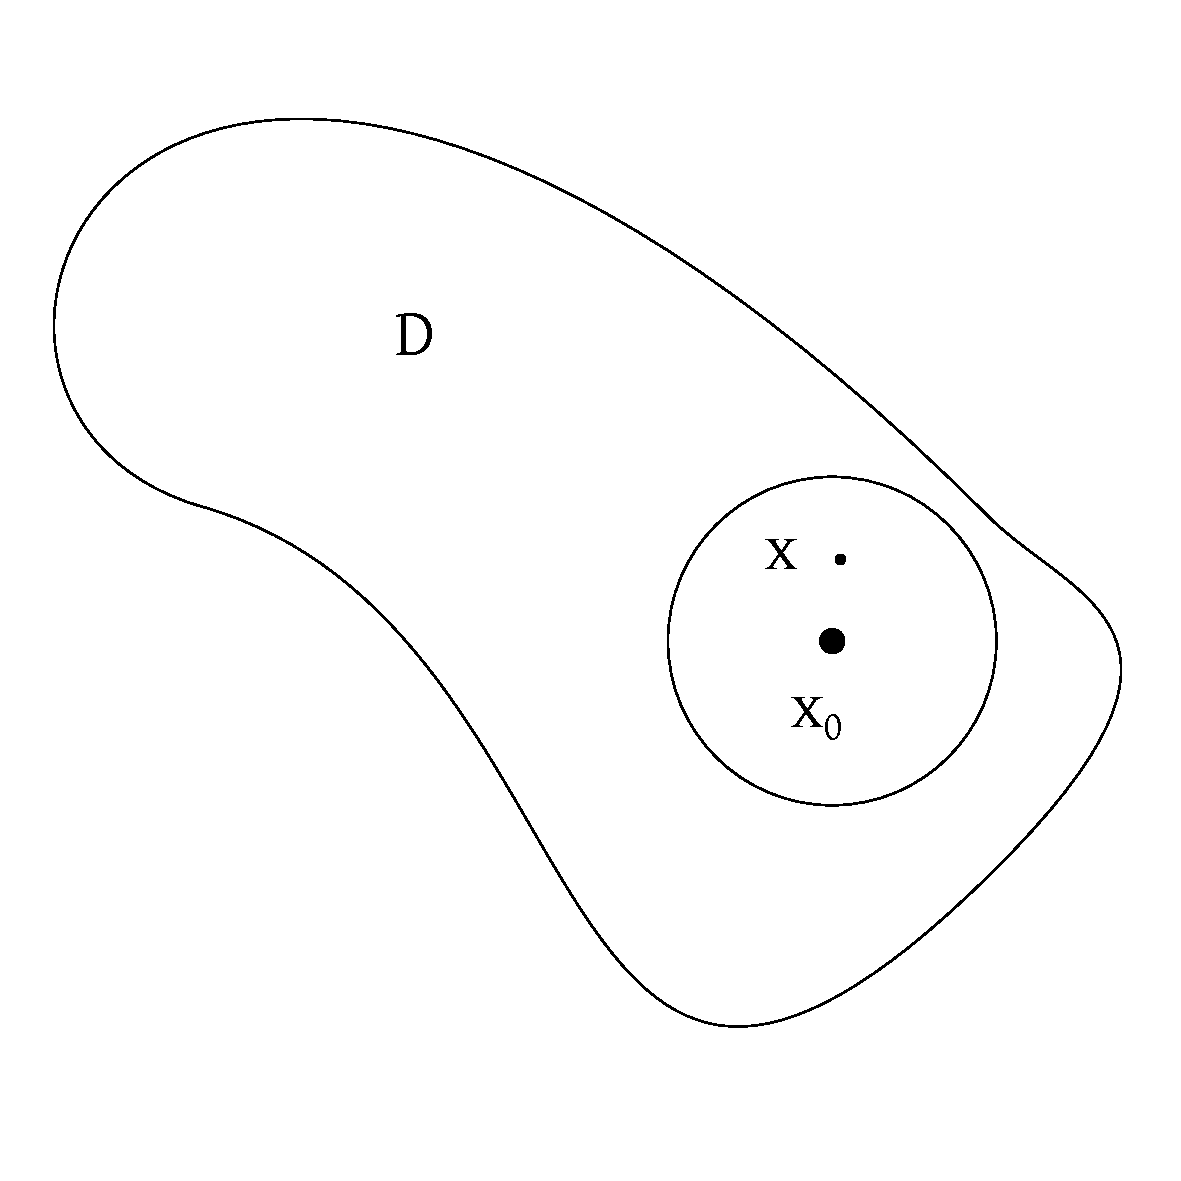
\includegraphics[width=0.3\textwidth]{img/D.pdf}
    \caption{Open set $D$}
  \end{center}
\end{figure}

\begin{lemma}
  Let $f, g: D \to \mathbb R^m$, $D \subseteq \mathbb R^n$ open.
  Let $f$ and $g$ be differentiable in $x_0$.
  Then for $\lambda \in \mathbb R$, $\lambda \cdot f$ is also differentiable in $x_0$.
  and $f + g$ is differentiable in $x_0$ with
  \[ D(\lambda f) (x_0) = \lambda Df(x_0) \]
  \[ D(f + g)(x_0) = Df(x_0) + Dy(x_0) \]
  Hence the derivative operator $D$ applies linearly on the function.
\end{lemma}
\begin{proof}
  \begin{align*}
    &\norm{\lambda f(x) - \lambda f(x_0) - \lambda Df(x_0) \cdot (x - x_0)}_{\mathbb K^m} \\
    &= \abs{\lambda} \cdot \norm{f(x) - f(x_0) - Df(x_0) \cdot (x - x_0)}_{\mathbb R^m} \\
    &= \underbrace{\abs{\lambda} \cdot r(x - x_0)}_{\lim_{x\to x_0} r(x- x_0) = 0} \cdot \norm{x - x_0} \text{with} \lim_{x\to x_0} r(x - x_0) = 0 = o(x - x_0)
  \end{align*}
  \[
  \leq \underbrace{\norm{f(x) - f(x_0) - Df(x_0) (x - x_0)}_{\mathbb R^m}}_{o(x - x_0)} +
  \underbrace{\norm{g(x) - g(x_0) - Dg(x_0) (x - x_0)}_{\mathbb R^m}}_{o(x - x_0)}
  \] \[
  = o(x - x_0)
  \]
\end{proof}

\begin{rem}
  Let $A: \mathbb R^n \to \mathbb R^m$ be linear.
  We identify $A$ with the matrix representation of $A$ in regards of canonical bases in $\mathbb R^m$
  (or $\mathbb R^n$).
\end{rem}

\index[English]{Matrix norm}
\index[German]{\foreignlanguage{ngerman}{Matrix norm}}
\begin{defi}[Matrix norms]
  Let $X$ and $Y$ be vector spaces. Then $\mathcal{L}(X, Y) = \operatorname{Hom}(X, Y) = \setdef{A}{A: X \to Y \text{ is linear}}$
  is also a vector space.
  A norm on $\mathcal{L}(\mathbb R^n, \mathbb R^m) = \mathbb R^{m\times n}$ is called \emph{matrix norm}.
\end{defi}

\begin{ex}
  Let $A = [a_{ij}]_{\substack{i = 1, \ldots, m \\ j = 1, \ldots, n}}$ be an $m \times n$ matrix.
  We let $\norm{A}_{F} = \left(\sum_{i=1}^m \sum_{j=1}^n a_{i,j}^2\right)^{\frac 12}$.
  $\norm{.}_F$ is called Forbeniusnorm in $A$. $\norm{.}_F$ is a matrix norm.
\end{ex}

\index[English]{Operator norm}
\index[German]{\foreignlanguage{ngerman}{Operatorennorm}}
\begin{defi}
  Let $A: \mathbb R^n \to \mathbb R^m$ be linear and let $\norm{.}_{\mathbb R^n}$ and $\norm{.}_{\mathbb R^m}$ be chosen.
  Then we define
  \[ \norm{A} = \sup_{V \neq \vec{0}}{\norm{A \frac{V}{{\norm{V}}_{\mathbb R^n}}}_{\mathbb R^m}} \]
  and we call $\norm{A}$ the \emph{operator norm} of $A$ in regards of $\norm{.}_{\mathbb R^n}$ and $\norm{.}_{\mathbb R^m}$.
\end{defi}

\begin{lemma}
  Let $\norm{.}_{\mathbb R^n}$ and $\norm{.}_{\mathbb R^m}$ be chosen norms.
  Let $A: \mathbb R^n \to \mathbb R^m$ be linear. Then it holds that
  \begin{enumerate}
  \item $h(w) = \norm{w}_{\mathbb R^m}$ is a continuous map
    \[ h: (\mathbb R^m, \norm{.}_{\mathbb R^m}) \to \mathbb R^+ \]
  \item
    \[ \norm{A} = \sup_{V \neq 0} \norm{A \cdot \frac{V}{\norm{V}_{\mathbb R^n}}}_{\mathbb R^m} \]
    \[ \max_{\substack{x \in \mathbb R^n \\ \norm{x}_{\mathbb R^n} = 1}} \norm{A \cdot x}_{\mathbb R^m} \]
  \end{enumerate}
\end{lemma}

\begin{proof}
  \begin{enumerate}
  \item
    Let $\varepsilon > 0$ be arbitrary.
    \[ \abs{h(w_1) - h(w_2)} = \abs{\norm{w_1}_{\mathbb R^m} - \norm{w_2}_{\mathbb R^m}} \]
    \[ \overset{\text{inv. triangle ineq.}}{\leq} \norm{w_1 - w_2}_{\mathbb R^m} < \varepsilon \text{ if } \norm{w_1 - w_2} < \varepsilon \]
  \item
    Let $x \in S^{n-1}_{\norm{.}_{\mathbb R^n}} = \setdef{x \in \mathbb R^n}{\norm{x}_{\mathbb R^n} = 1}$.
    Then it holds that
    \[ \norm{Ax}_{\mathbb R^n} = \norm{A \frac{x}{\norm{x}_{\mathbb R^n}}}_{\mathbb R^m}
       \leq \sup_{\substack{V \in \mathbb R^n \\ V \neq 0}} \norm{A \frac{V}{\norm{V}_{\mathbb R^n}}} = \norm{A} \]
    So it also holds
    \[ \sup_{x \in S^{n-1}_{\norm{.}_{\mathbb R^n}}} \norm{Ax} \leq \norm{A} \]
    On the opposite, let $v \in \mathbb R^n$ with $v \neq 0$ arbitrary.
    Then it holds that $z = \frac{V}{\norm{V}}_{\mathbb R^n} \in S^{n-1}_{\norm{.}_{\mathbb R^n}}$
    and
    \[ \norm{A \frac{V}{\norm{V}_{\mathbb R^n}}} = \norm{A z}_{\mathbb R^m} \leq \sup_{\norm{x}_{\mathbb R^n} = 1} \norm{Ax}_{\mathbb R^m} \]
    \[ \implies \norm{A} = \sup_{\substack{V \neq 0 \\ V \in \mathbb R^n}} \norm{A \cdot \frac{V}{\norm{V}_{\mathbb R^n}}} \leq \sup_{\norm{x}_{\mathbb R^n} = 1} \norm{Ax}_{\mathbb R^m} \]
    So it holds that
    \[ \sup_{\substack{V \neq 0 \\ V \in \mathbb R^n}} \norm{A \frac{V}{\norm{V}_{\mathbb R^n}}}_{\mathbb R^m} = \sup_{\substack{x \in \mathbb R^n \\ \norm{x}_{\mathbb R^n} = 1}} \norm{Ax}_{\mathbb R^m} \]
    It remains to show: right-sided $\sup$ is maximum.

    We consider: $f: S^{n-1}_{\norm{.}_{\mathbb R^n}} \to \mathbb R$.
    \[ f(x) = \norm{Ax}_{\mathbb R^m} = h \circ A(x) \]
    Linear maps $A \in \mathcal{L}(\mathbb R^n, \mathbb R^m)$ are continuous,
    $h$ is continuous. Hence $f$ is continuous and takes the maximum value in compact set $S^{n-1}_{\norm{.}_{\mathbb R^n}}$.
  \end{enumerate}
\end{proof}

\begin{rem}
  Equivalent definition: Recall: $\sup_2\set{M}$.

  $M \subseteq \mathbb R$ is the smallest upper bound of $M$.

  Hence $\norm{A} = \inf\set{\tilde{m} \geq 0: \norm{A \frac{V}{\norm{V}_{\mathbb R^n}}}_{\mathbb R^m} \leq \tilde{m} \quad \forall v \in \mathbb R^n \setminus \set{0}}$
  \[ = \inf\set{\tilde{m} \geq 0: \underbrace{\norm{Av}_{\mathbb R^m} \leq \tilde{m} \norm{v}_{\mathbb R^n}}_{*}} \]
  $*$ holds anyways for $v = 0$.

  So $\norm{A}$ is the smallest constant $\tilde{m}$ such that
  \[ \norm{A v}_{\mathbb R^m} \leq \tilde{m} \norm{v}_{\mathbb R^n} \]
  holds for all $v \in \mathbb R^n$. Especially it holds that
  \begin{mdframed}
    \[ \norm{Av}_{\mathbb R^n} \leq \norm{A} \cdot \norm{v}_{\mathbb R^n} \]
    \end{mdframed}
  (This only works for operator norms. A very important result.)
\end{rem}

\meta{lecture}{3rd of June 2016}{Wolfgang Ring}

\begin{rem}[Equivalent characterization of $\norm{A}$]
  \[ \norm{A} = \max_{\substack{x \in \mathbb R^n \\ \norm{x} = 1 \\ \mathbb R^n}} \norm{Ax}_{\mathbb R^m} = \max_{\substack{v \in \mathbb R^n \\ v \neq \vec{0}}} \frac{1}{\norm{v}_{\mathbb R^n}} \cdot \norm{Av}_{\mathbb R^m} \]
  \[ = \min\set{\tilde{m}: \norm{Av}_{\mathbb R^m} \leq  \tilde{m} \norm{v}_{\mathbb R^n} \forall v \in \mathbb R^n} \]
\end{rem}

\begin{lemma}
  Let $A \in \mathcal{L}(\mathbb R^n, \mathbb R^m)$. Then $A$ is continuous in $\mathbb R^n$.
\end{lemma}
\begin{proof}
  Consider linear $A: \mathbb R^n \to \mathbb R^m$. We know that $A$ is continuous if and only if component $A^j$ is continuous as map from $\mathbb R^n \to \mathbb R$ (for $i=1,\ldots,m$).
  \[ A^i(x) = \sum_{j=1}^n a_{ij} x_j \]
  Choose $\norm{.}_2$ in $\mathbb R^n$ and $\abs{.}$ in $\mathbb R$.
  Show: Component $A^i$ is continuous for these norms.
  Let $x,y \in \mathbb R^n$. Then it holds that
  \[ \abs{A^i x - A^i y} = \abs{A^i (x - y)} = \sum_{j=1}^n a_{ij} (x_j - x_i) \]
  \[ = \langle a^i, x - y\rangle \overset{\text{Cauchy-Schwarz}}{\leq} \norm{a^i}_2 \cdot \norm{x - y}_2  \]
  So $A^i$ is Lipschitz continuous and therefore continuous.
\end{proof}

\begin{cor}[Conclusion of estimate $\norm{Ax} \leq \norm{A} \norm{x}$]
  The function $A: \mathbb R^n \to \mathbb R^m$ is Lipschitz continuous with Lipschitz constant $\norm{A}$.

  Obvious, because $\norm{A(x-y)} \leq \norm{A} \cdot \norm{x-y}$.
\end{cor}

\begin{rem}
  These law only hold for operator norms.
  This estimate also defines \emph{boundedness}.
  Bounded equals linear for operator norms.
\end{rem}

\begin{lemma}
  Let $\norm{A}$ be an operator norm in $\mathcal{L}(\mathbb R^n, \mathbb R^m)$.
  Then $\norm{A}$ is a norm in $\mathcal{L}(\mathbb R^n, \mathbb R^m)$.
\end{lemma}
\begin{proof}
  \begin{enumerate}
    \item
      \begin{align*}
        \norm{A} = 0 &\iff \max\set{\frac{1}{\norm{v}} \norm{Av}: v \in \mathbb R^n, v \neq 0} = 0 \\
          &\iff \frac{1}{\norm{v}} \norm{Av} = 0 \forall v \in \mathbb R^n, v \neq \vec{0} \\
          &\iff \norm{Av} = 0 \forall v \neq \vec{0} \iff A = \underbrace{0}_{\text{zero matrix}}
      \end{align*}
    \item \begin{align*}
        \norm{\lambda A} &= \max\set{\norm{\lambda Ax}: \norm{x} = 1} \\
          &= \abs{\lambda} \cdot \max{\norm{Ax}: \norm{x} = 1} = \abs{\lambda} \cdot \norm{A}
      \end{align*}
    \item
      Let $x \in \mathbb R^n$ with $\norm{x} = 1$ arbitrary. $A,B \in \mathcal{L}(\mathbb R^n, \mathbb R^m)$.
      Then it holds that
      \[ \norm{(A+B)x} \overset{\text{triangle ineq. in $\mathbb R^m$}}{\leq} \norm{Ax} + \norm{Bx} \leq \norm{A} \underbrace{\norm{x}}_{=1} + \norm{B} \underbrace{\norm{x}}_{=1} \]
      \[ = \norm{A} + \norm{B} \]
      \[ \implies \forall x \in \mathbb R^n: \norm{(A+B)x} \leq \norm{A} + \norm{B} \]
      \[ \implies \underbrace{\max\set{\norm{(A+B)x}: \norm{x} = 1}}_{\norm{A+B}} \leq \norm{A} + \norm{B} \]
  \end{enumerate}
\end{proof}

\begin{lemma}
  Let $A = \set{\mathbb R^n, \mathbb R^m}$ and $B \in \mathcal{L}(\mathbb R^m, \mathbb R^n)$.
  Choose fixed norms in $\mathbb R^n$, $\mathbb R^m$, $\mathbb R^l$.
  Let $\norm{A}$ be the operator norm of $A$ in regards of $\norm{.}_{\mathbb R^n}$ and $\norm{.}_{\mathbb R^m}$.
  Let $\norm{B}$ be the operator norm of $B$ in regards of $\norm{.}_{\mathbb R^n}$ (like for $\norm{A}$!) and $\norm{.}_{\mathbb R^l}$.
  Then it holds that
  \[ \norm{BA} \leq \norm{B} \norm{A} \]
\end{lemma}
\begin{proof}
  \[ \norm{BA} = \max\set{\underbrace{\norm{BAx}_{\mathbb R^l}}_{\leq \norm{B} \cdot \norm{Ax}}: \norm{x} = 1} \]
  \[ \leq \norm{B} \cdot \underbrace{\max\set{\norm{Ax}: \norm{x} = 1}}_{= \norm{A}} = \norm{B} \cdot \norm{A} \]
\end{proof}

\subsection{Returning to differential calculus in $\mathbb R^n$}
%
\begin{theorem}[Chain rule in multiple dimensions]
  Let $f: O \subseteq \mathbb R^n \to \mathbb R^m$.
  Let $U \subseteq \mathbb R^m$ be open and $g: U \to \mathbb R^l$ and $f(O) \subseteq U$.

  \begin{figure}[!h]
    \begin{center}
      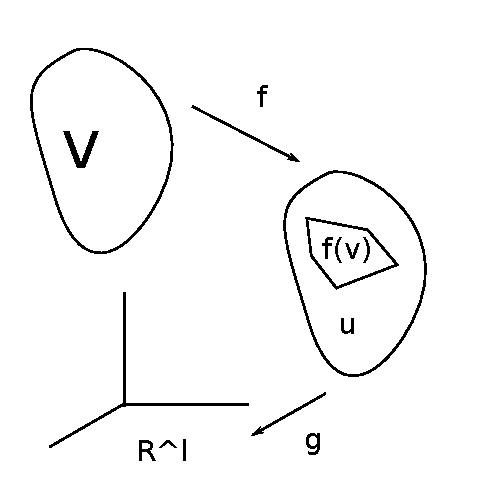
\includegraphics{img/multiple_dimension_chain_rule.pdf}
      \caption{Chain rule in multiple dimensions}
      \label{img:chain-rule}
    \end{center}
  \end{figure}

  Let $f$ in $x_0 \in O$ differentiable and $y$ in $y_0 = f(x_0) \in U$ differentiable.
  Then $g \circ f$ in $x_0$ is differentiable and it holds that
  \[ D(g \circ f)(x_0) = Dg(y_0) \cdot Df(x_0) = \underbrace{Dg(f(x_0))}_{\in \mathbb R^{l\times m}} \cdot \underbrace{Df(x_0)}_{\in \mathbb R^{m\times n}} \]
\end{theorem}
\begin{proof}
  Let $\varepsilon > 0$ be arbitrary.
  Show that
  \[ \frac{1}{\norm{x - x_0}} \norm{g(f(x)) - g(f(x_0)) - Dg(f(x_0)) \cdot Df(x_0) (x - x_0)} = r (x - x_0) < \varepsilon \]
  for sufficiently small $\norm{x - x_0}$.
  \[ \frac{1}{\norm{x - x_0}} \| g(f(x)) - g(f(x_0)) \mp Dg(f(x_0)) \cdot (f(x) - f(x_0)) \]\[ - Dg(f(x_0)) \cdot Df(x_0) (x - x_0)\| \]
  \[ \leq \frac{1}{\norm{x - x_0}} \norm{g(f(x)) - g(f(x_0)) - Dg(f(x_0)) (f(x) - f(x_0))} \]
  \[ + \frac{1}{\norm{x - x_0}} \norm{Dg(f(x_0)) \cdot \left(f(x) - f(x_0) - Df(x_0) (x - x_0)\right)} \]
  \[ \leq \frac{1}{\norm{x - x_0}} \norm{\overbrace{g(f(x)) - g(f(x_0)) - Dg(f(x_0)) (f(x) - f(x_0))}^{\text{small, because }g\text{ is differentiable in }f(x_0)}} \]
  \[ + \frac{1}{\norm{x - x_0}} \norm{Dg(f(x_0))} \cdot \underbrace{\norm{f(x) - f(x_0) - Df(x_0) \cdot (x - x_0)}}_{\text{small, because $f$ is differentiable in $x_0$}} \]
  Remember those expressions as (\#).

  First, choose $\delta_1$ such that
  \[ \norm{f(x) - f(x_0) - Df(x_0) (x - x_0)} \leq 1 \cdot \norm{x - x_0} \]
  for all $\norm{x - x_0} < \delta_1$, $x \in O$.
  Possible, because $f$ is differentiable in $x_0$.
  \[ \implies \frac{\norm{f(x) - f(x_0)}}{\norm{x - x_0}} < 1 + \norm{Df(x_0)} \]
  Choose $\delta_g$ such that $\norm{y - y_0} < \delta_g$ (with $f(x_0) = y_0$) such that
  \[ \norm{g(y) - g(y_0) - Dg(y_0) (y - y_0)} \leq \frac\varepsilon2 \frac{1}{\norm{Df(x_0)} + 1} \norm{y - y_0} \]
  is possible, because $g$ is differentiable in $y_0$.
  The inequality above also holds for $y = y_0$.
  Let $\delta_2$ such that for all $\norm{x - x_0} < \delta_2 \implies \norm{f(x) - f(x_0)} < \delta_g$.
  This is possible, because $f$ is continuous in $x_0$
  (and $f$ differentiable in $x_0 \implies f$ is continuous in $x_0$).

  Now let $\norm{x - x_0} < \min\set{S_1, S_2}$. Then it holds that
  \[ \frac{1}{\norm{x - x_0}} \cdot \norm{g(f(x)) - g(f(x_0)) - Dg(y_0)\left(\underbrace{f(x) - f(x_0)}_{\norm{f(x) - f(x_0)} < \delta g}\right)} \]
  \[ \leq \frac{\varepsilon}{2} \frac{1}{\norm{x - x_0}} \frac{1}{\norm{Df(x_0)} + 1} \underbrace{\norm{f(x) - f(x_0)}}_{\leq (\norm{Df(x_0)} + 1)\norm{x - x_0}} < \frac{\varepsilon}{2} \]
  The expression in underbrace holds by choice of $\delta_1$.
  Now let $\delta_3 > 0$ such that
  \[ \norm{x - x_0} < \delta_3
  \implies \frac{1}{\norm{x - x_0}} \norm{f(x) - f(x_0) - Df(x_0)(x - x_0)} \]
  \[ < \frac{1}{\norm{Dg(f(x_0)) + 1}} \frac{\varepsilon}{2} \]
  is possible, because $f$ is differentiable in $x_0$.
  So it holds that $\norm{x - x_0} < \delta_3$.
  \[ \frac{1}{\norm{x - x_0}} \norm{Dg(y_0)} \cdot \norm{f(x) - f(x_0) - Df(x_0)(x - x_0)} \]
  \[ < \norm{Dg(y_0)} \cdot \frac{\varepsilon}{2} \cdot \frac{1}{\norm{Dg(y_0)} + 1} < \frac{\varepsilon}{2} \]
  For $\norm{x - x_0} < \min{\delta_1, \delta_2, \delta_3}$ every expression from (\#)
  is smaller than $\frac\varepsilon2$. The desired inequality was proven.
\end{proof}

\begin{lemma}
  Let $f: D \subseteq \mathbb R$ where $D$ is open and $x_0 \in D$.
  If $f$ is differentiable in $x_0$, then $f$ is also continuous in $x_0$.
\end{lemma}
\begin{proof}
  Let $\varepsilon > 0$ be arbitrary.
  \[ \norm{f(x) - f(x_0)} \leq \overbrace{\norm{f(x) - f(x_0) - Df(x_0)(x - x_0)}}^{r(x - x_0) \norm{x - x_0}} + \norm{Df(x_0) (x - x_0)} \]
  \[ \leq r (x - x_0) \norm{x - x_0} + \norm{Df(x_0)} \cdot \norm{x - x_0} \]
  Choose $\delta > 0$ such that
  \begin{enumerate}
  \item $\delta < \frac\varepsilon2 \left(\norm{Df(x_0)} + 1\right)^{-1} \leq \frac{\varepsilon}{2}$
  \item for $\norm{x - x_0} < \delta \implies r(x - x_0) \leq 1$
  \end{enumerate}
  Let $\norm{x - x_0} < \delta$. Then it holds that
  \[ \norm{f(x) - f(x_0)} \leq 1 \cdot \frac{\varepsilon}{2} + \norm{Df(x_0)} \cdot \frac{\varepsilon}{2} \frac{1}{\norm{Df(x_0)} + 1} < \frac{\varepsilon}{2} + \frac{\varepsilon}{2} = \varepsilon \]
  Hence $f$ is continous in $x_0$.
\end{proof}

\index[English]{Differentiability in $\mathbb R^n$}
\index[German]{\foreignlanguage{ngerman}{Ableitbarkeit in $\mathbb R^n$}}
\begin{defi}
  Let $f: D \subseteq \mathbb R^n \to \mathbb R^m$ a function.
  We state: $f$ is \emph{differentiable in $D$}, if $f$ is
  differentiable in every point $x_0 \in D$. The map
  \[ x \mapsto Df(x) \]
  \[ D \to \mathbb R^{m\times n} \]
  is called \emph{derivative function of $f$}.

  We say $f$ is \emph{continuously differentiable in $D$}
  if the derivative function $x \mapsto Df(x)$ is continuous in terms of $\norm{.}_{\mathbb R^n}$ in $\mathbb R^n$ and
  in terms of the operator norm in $\mathbb R^{m\times n}$.

  Hence,
  \[ \forall \varepsilon > 0 \exists \delta > 0:
  \left[\norm{x - x_0} < \delta \text{ and } x \in D \implies \norm{Df(x) - Df(x_0)} < \varepsilon\right]
  \]
\end{defi}

\begin{rem}
  $f$ is continuously differentiable in $\overline{D}$,
  if every point of $\overline{D}$ is a limit point (dt. \enquote{H\"aufungspunkt}) in $D$ and
  in every point $x_0 \in \overline{D}$ the differentiability condition
  \[ \norm{f(x) - f(x_0) - Df(x_0)(x - x_0)} = o(x - x_0) \]
  holds and $x \mapsto Df(x)$ is a continuous function on $\overline{D}$.
\end{rem}

\section{Computing $Df(x_0)$}
%
\[ \lim_{v \to 0} \frac{f(x_0 + v) - f(x_0)}{v} = ? \]

\index[English]{Gateaux derivative}
\index[German]{\foreignlanguage{ngerman}{Gateaux Ableitung}}
\begin{defi}
  Let $f: D \to \mathbb R^m$ be given.
  Let $D \subseteq \mathbb R^n$ be open.
  Let $x_0 \in D$ and $v \in \mathbb R^n \setminus \set{\vec{0}}$.
  We define
  \[ df(x_0; v) = \lim_{t\to 0} \frac1{t} \left(f(x_0 + tv) - f(x_0)\right) \]
  if the limit exists.

  In this case we call $df(x_0; v)$ the directional derivative (\emph{G\^ateaux derivative})
  of $f$ in direction $v$ in point $x_0$. Compare with Figure~\ref{img:gatder}.
\end{defi}

\begin{figure}[t]
  \begin{center}
    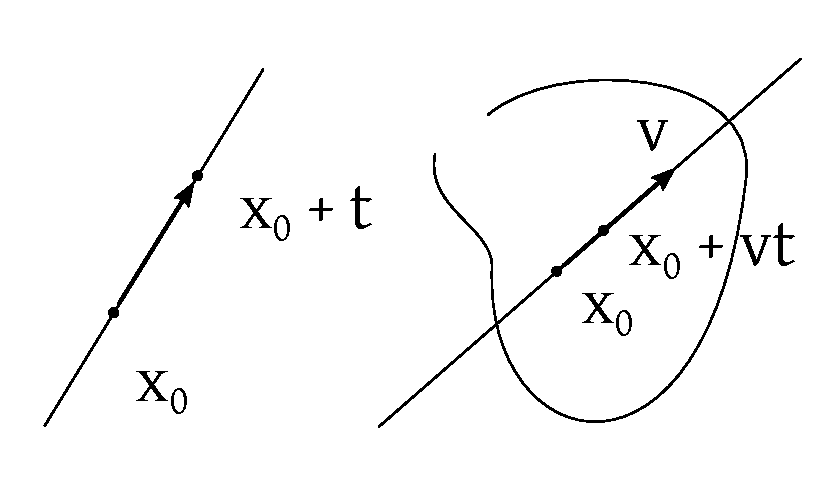
\includegraphics[width=0.4\textwidth]{img/Gateaux_derivative.pdf}
    \caption{Directional derivative and Gateaux derivative}
    \label{img:gatder}
  \end{center}
\end{figure}

\begin{rem}
  Let $l_{x_0,v}(t) = x_0 + t \cdot v$ (parameter form of a straight line).
  \[ l_{x_0,v}: \mathbb R \to \mathbb R^n \]
  is linear affine (constant and linear).
  $l_{x_0,v}$ is differentiable in $\mathbb R$.
  Furthermore it holds (by chain rule) that $f(x_0 + t\cdot v) = f \circ l_{x_0,v}(t)$
  defines an environment of $t = o$.
  \[ df(x_0;v) = D(f \circ l_{x_0,v}) (0) \]
  \[ Dl_{x_0;v}(0) = v \in \mathbb R^n \quad \text{ column vector} \]
  If $f$ is Frech\'et differentiable in $x_0$, then it holds (by the chain rule)
  \[ df(x_0; v) = Df(l_{x_0,v}(0)) \cdot Dl_{x_0,v}(0) = Df(x_0) \cdot v \]
\end{rem}

\begin{lemma}
  Let $f$ be like above and Frech\'et differentiable in $x_0$. Then it holds that
  \[ df(x_0;v) = Df(x_0) \cdot v \]
  Now I can build the columns of $Df$.
\end{lemma}

\meta{lecture}{7th of June 2017}{Wolfgang Ring}

\subsection{Special directional derivatives}

\begin{rem}[Reminder]
  We write indices for coordinates as superscript
  (notation originates in differential geometry).
  But in the following we also which to subscript,
  which is more convenient under some circumstances.
\end{rem}

\index[English]{$k$-th partial derivative of $f$ in $x_0$}
\index[German]{\foreignlanguage{ngerman}{$k$-te partielle Ableitung von $f$ in $x_0$}}
\begin{defi}
  Let $v = e_k$ where $1$ is at the $k$-th index;
  i.e. $k$-th canonical basis vector in $\mathbb R^n$.

  \[
    df(x_0, e_l) = \lim_{t\to 0} \frac1{t} \left(f(x_0 + t \cdot e_k) - f(x_0)\right)
    \text{ with } \begin{bmatrix} 0 \\ \vdots \\ 1 \\ \vdots \\ 0 \end{bmatrix}
  \] \[
    = \lim_{t \to 0} \frac{1}{t} \left(f(x_0^1, x_0^2, \ldots, x_0^k + t, x_0^{k-1}, \ldots, x_0^n) - f(x_0^1, \ldots, x_0^n)\right)
  \] \[
    = \frac{\partial f}{\partial x^k} = f_{x^k} = f_k = \partial_k f
  \]
  is called \emph{$k$-th partial derivative of $f$ in $x_0$}.
\end{defi}

\subsection{Determination of partial derivatives}
%
In the $k$-th derivative, $x^1, \ldots, x^{k-1}, x^{k+1}, \ldots, x^n$ are treated like constants.
Derivative rules are applied to the \enquote{variable} $x^k$.

An example:
\[
f(x^1, x^2, x^3) =
\begin{bmatrix}
  x^1 (x^3)^2 + \sin(x^2 x^3) \\
  \frac{(x^2)^2}{(x^1)^2 + 1}
\end{bmatrix}
\]
where $x^2$ is the derivative variable. Then:
\[
\partial_2 f(x_0^1, x_0^2, x_0^3) =
\begin{bmatrix}
  \cos(x^2 \cdot x^3) \cdot x^3 \\
  \frac{2x^2}{(x^1)^2 + 1}
\end{bmatrix}
\]

\index[English]{Jacobi matrix}
\index[German]{\foreignlanguage{ngerman}{Jacobi Mmatrix}}
\begin{theorem}
  Let $f: D \to \mathbb R^m$, $D$ is open in $x_0 \in D$ differentiable.
  Then it holds that
  \[ Df(x_0) = \left(\partial_j f^i(x_0)\right)_{\substack{i = 1,\ldots,m \\ j = 1,\ldots,n}} \in \mathbb R^{m\times n} \]
  \[ \left(\partial_j f^i(x_0)\right)_{\substack{i=1,\ldots,m \\ j = 1,\ldots,m}} \]
  is called \emph{Jacobi matrix} of $f$ in $x_0$.
\end{theorem}

\begin{proof}
  The matrix representation of the linear map $Df(x_0)$ in regards of canonical bases
  in $\mathbb R^n$ (or equivalently $\mathbb R^m$) contains the vector
  $Df(x_0) \cdot e_k = df(x_0; e_k)$ in the $k$-th column.

  \[
    df(x_0, e_k) = \partial_k f = \begin{bmatrix} \partial_k f^1 \\ \partial_k f^2 \\ \vdots \\ \partial_k f^m \end{bmatrix}
    \implies (Df(x_0))_{i,k} = \partial_k f^i(x_0)
  \]
\end{proof}

\begin{ex}
  \[
    f: \mathbb R^3 \to \mathbb R^2: f(\underbrace{x_1, x_2, x_3}_{\begin{bmatrix} x_1 \\ x_2 \\ x_3 \end{bmatrix}}) =
    \begin{bmatrix}
      x_1 x_3^2 + \sin(x_2 \cdot x_3) \\
      \frac{x_2^2}{x_1^2 + 1}
    \end{bmatrix}
  \] \[
  Df\left(\begin{bmatrix} x_1 \\ x_2 \\ x_3 \end{bmatrix}\right) =
  \begin{bmatrix}
    x_3^2                                   & \cos(x_2 x_3) \cdot x_3                & 2x_2 x_3^2 + \cos(x_2 x_3) \cdot x_2 \\
    - \frac{x_2^2}{(x_1^2 + 1)} \cdot 2x_1   & \frac{2x_2}{x_1^2 + 1} \cdot 2x_1      & 0
  \end{bmatrix}
  \]
\end{ex}

\begin{theorem}
  Let $D \subset \mathbb R^n \to \mathbb R^m$ and $D$ is open.
  \[
    f(x) = \begin{bmatrix}
      f^1(x) \\ \vdots \\ f^m(x)
    \end{bmatrix}
  \]
  Then if $f$ is differentiable in $x_0 \in D$,
  then $f^j: D \to \mathbb R$ in $x_0$ is differentiable for $j = 1, \ldots, m$.
\end{theorem}
\begin{proof}
  $f$ is differentiable in $x_0$ iff
  \[\forall \varepsilon > 0 \exists \delta > 0: \norm{x - x_0} < \delta \]
  \[ \implies \inorm{f(x) - f(x_0) - Df(x_0) (x - x_0)} < \varepsilon \norm{x - x_0} \]

  \[ \iff \forall \varepsilon > 0 \exists \delta > 0: \norm{x - x_0} < \delta \]
  \[ \implies \abs{f^0(x) - f^0(x_0) - \sum_{k=1}^m \partial_k f^j(x_0)(x^k - x_0^k)} < \varepsilon \norm{x - x_0} \]
  \[ \text{ for } j = 1, \ldots, m \]

  $\iff$ $f^j$ is Fr\'echet differentiable in $x_0$ with derivative
  \[ Df^j(x_0) = [\partial_1 f^1, \partial_2 f^2, \ldots, \partial_n f^j](x_0) \]

  Additionally,
  \[ Df^j(x_0) = [\partial_1 f^j(x_0), \ldots, \partial_n f^j(x_0)] \]
\end{proof}

\index[English]{Total differential of $f$ in $x_0$}
\index[German]{\foreignlanguage{ngerman}{Totales Differential von $f$ in $x_0$}}
\index[English]{Gradient vector of $f$ in $x_0$}
\index[German]{\foreignlanguage{ngerman}{Gradientenvektor von $f$ in $x_0$}}
\index[English]{Nabla operator}
\index[German]{\foreignlanguage{ngerman}{Nablaoperator}}
\begin{rem}
  For many considerations we can look at the
  special case $f: D \subseteq \mathbb R^n \to \mathbb R$.

  \emph{Notation:} Let $f: D \subseteq \mathbb R^m \to \mathbb R$
  be given and differentiable in $x_0 \in D$.
  \begin{align*}
    Df(x_0) &= [\partial_1 f(x_0), \ldots, \partial_n f(x_0)] \\
            &= df(x_0)
  \end{align*}
  is also called \emph{total differential of $f$ in $x_0$} (a row vector).

  \[ Df(x_0) \cdot v = df(x_0; v) = [\partial_1 f(x_0), \ldots, \partial_n f(x_0)] \begin{bmatrix} v_1 \\ \vdots \\ v^n \end{bmatrix} \]
  We let
  \[
  \nabla f(x_0) = \begin{bmatrix} \partial_1 f(x_0) \\ \vdots \\ \partial_n f(x_0) \end{bmatrix}
  = (Df(x_0))^t
  \]
  is called \emph{gradient vector of $f$ in $x_0$} ($\nabla$ of the Old Greek alphabet is called \emph{nabla}).

  With this notation it holds that the directional derivative
  \[ Df(x_0) \cdot v = \langle \nabla f(x_0), v\rangle \]

  The reason for different notations is coordinate transformation.

  \begin{figure}[h]
    \begin{center}
      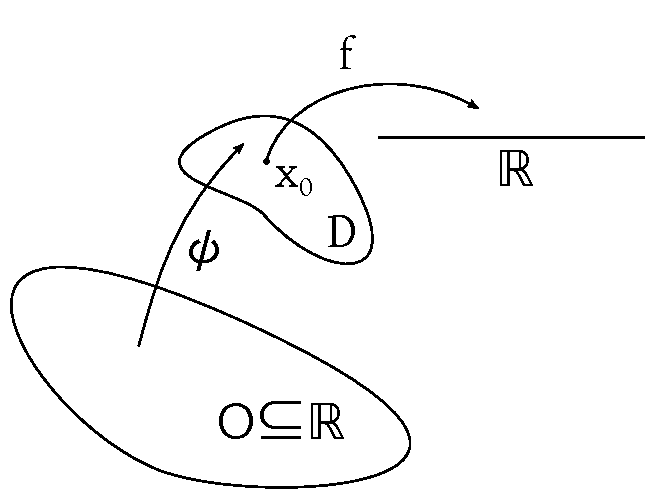
\includegraphics[width=0.4\textwidth]{img/coordinate_transformation.pdf}
      \caption{Coordinate transformation}
      \label{img:coordtrans}
    \end{center}
  \end{figure}
  This is illustrated in Figure~\ref{img:coordtrans} with $f: O \to D$ is differentiable everywhere and bijective.
  \[ f: 0 \to D \]
  is differentiable everywhere and bijective.
  \[ x = \varphi(y) \qquad x_0 = \varphi(y_0) \qquad \tilde{f} = f \circ \varphi: O \to \mathbb R \]
  Coordinate transformation of $f$.
  \[ D\tilde{f}(y_0) \underbrace{=}_{\text{chain rule}} Df(x_0) \cdot \underbrace{D\varphi(y_0)}_{\text{transformation by $D\varphi$}} \]
  \begin{align*}
    D\tilde{f}(y_0) &= \left(Df(x_0) \cdot D\varphi(y_0)\right)^t \\
    &= D\varphi^t(y_0) \cdot Df(x)^t \\
    &= D\varphi^t(y_0) \cdot \nabla f(x_0)
  \end{align*}

  \index[English]{Covariant transformation behavior}
  \index[German]{\foreignlanguage{ngerman}{Kovariantes Transformationsverhalten}}
  \index[English]{Contravariant transformation behavior}
  \index[German]{\foreignlanguage{ngerman}{Kontravariantes Transformationsverhalten}}

  Transformation behavior of $Df$ and $\nabla f$ is different.
  $Df$ is a covariant vector (covector) and $\nabla f$ is a contravariant vector (vector).
\end{rem}

Question: If all partial derivatives of a function exist, is $f$ differentiable? \\
Answer: In general no.

\begin{ex}[Counterexample]
  \[ f(x_1, x_2) = \begin{cases}
    x_1 \cdot \frac{x_1 x_2}{x_1^2 + x_2^2} & \text{ for } (x_1, x_2) \neq (0, 0) \\
    0                                     & \text{ for } (x_1, x_2) = (0, 0)
  \end{cases} \]
  $\partial_1 f$ and $\partial_2 f$ exist for $(x_1, x_2) \neq (0, 0)$.
  Consider directional derivatives of $f$ in point $\begin{bmatrix} 0 \\ 0 \end{bmatrix}$.
  Let $v = \begin{bmatrix} v_1 \\ v_2 \end{bmatrix}$.
  \[
  df(\vec{0}, v) = \lim_{t\to 0} \frac{f(t \cdot v) - 0}{t}
  = \lim_{t\to 0} \frac1{t} \left(tv_1 \frac{tv_1 \cdot tv_2}{(tv_1)^2 + (tv_2)^2}\right)
  = v_1 \frac{v_1 v_2}{v_1^2 + v_2^2}
  \]
  Hence in $\begin{bmatrix} 0 \\ 0 \end{bmatrix}$ all directional derivatives
  in directions $v \neq \begin{bmatrix} 0 \\ 0 \end{bmatrix}$ exist.
  \[ \partial_1 f(\vec{0}) = df(\vec{0}, e_1) = 1 \cdot \frac{1 \cdot 0}{1^2 + 0^2} = 0 \]
  \[ \partial_2 f(\vec{0}) = df(\vec{0}, e_2) = 0 \cdot \frac{0 \cdot 1}{0^2 + 1^2} = 0 \]
  Hence, if $f$ would be differentiable in $0$, then
  \[ Df(0) = \begin{bmatrix} 0 & 0 \end{bmatrix} \]
  Now consider $v = e_1 + e_2$
  \[ df(\vec{0}, v) = Df(0) \cdot v = \begin{bmatrix} 0 & 0 \end{bmatrix} \begin{bmatrix} 1 \\ 1 \end{bmatrix} = 0 \]
  But the determination from above of $df(\vec{0}, \vec{v})$ holds.
  \[ df(\vec{0}, \vec{v}) = 1 \cdot \frac{1 \cdot 1}{1^2 + 1^2} = \frac12 \neq 0 \]
  Recommendation: Plot this graph!
\end{ex}

\begin{figure}[h]
  \begin{center}
    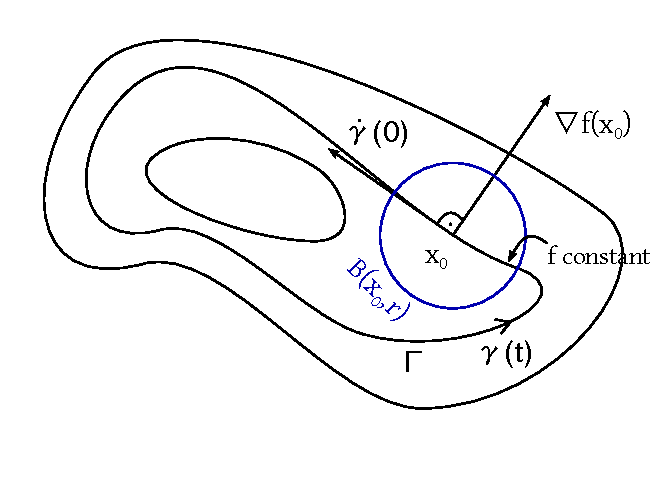
\includegraphics[width=0.4\textwidth]{img/level_lines.pdf}
    \caption{Directional derivative}
  \end{center}
\end{figure}

\begin{proof}[Show that $f$ is not differentiable]
  \[ f(\begin{bmatrix} x_1 \\ x_2 \end{bmatrix}) = \begin{cases}
    x_1 \cdot \frac{x_1 \cdot x_2}{x_1^2 + x_2^2}  & \text{ for } \begin{bmatrix} x_1 \\ x_2 \end{bmatrix} \neq \begin{bmatrix} 0 \\ 0 \end{bmatrix} \\
    0  & \text{ for } \begin{bmatrix} x_1 \\ x_0 \end{bmatrix} = \begin{bmatrix} 0 \\ 0 \end{bmatrix}
  \end{cases}
  \]
  We already know
  \[ \partial_1 f(\begin{bmatrix} 0 \\ 0 \end{bmatrix}) \neq \vec{0} \]
  Then it holds that
  \[ \partial_1 f(\begin{bmatrix} x_1 \\ x_2 \end{bmatrix}) = \frac{2 x_1 x_2 - x_1^2 x_2 \cdot 2x_1}{(x_1^2 + x_2^2)^2} \]
  \[ \partial_2 f(\begin{bmatrix} x_1 \\ x_2 \end{bmatrix}) = \frac{x_1^2 (x_1^2 + x_2^2) - x_1^2 \cdot x_2 \cdot 2x_2}{(x_1^2 + x_2^2)^2} \]
  \[ \partial_1 f(\begin{bmatrix} \varepsilon \\ \varepsilon \end{bmatrix}) =
    \frac{2 \varepsilon^2 \cdot 2 \varepsilon^2 - \varepsilon^2 \cdot \varepsilon \cdot 2\varepsilon}{(2 \varepsilon^2)^2} = \frac{2\varepsilon^4}{4 \varepsilon^4} = \frac12 \]
  \[ \partial_2 f(\begin{bmatrix} \varepsilon \\ \varepsilon \end{bmatrix}) = \frac{\varepsilon^2 \cdot 2\varepsilon^2 - \varepsilon^2 \cdot \varepsilon \cdot 2\varepsilon}{(2\varepsilon^2)^2} = 0 \]
  It holds that
  \[ \lim_{\varepsilon \to 0} \partial_2 f(\begin{bmatrix} \varepsilon \\ \varepsilon \end{bmatrix}) = 0 = \partial_2 f(\begin{bmatrix} 0 \\ 0 \end{bmatrix}) \]
  but
  \[ \lim_{\varepsilon \to 0} \partial_1 f(\begin{bmatrix} \varepsilon \\ \varepsilon \end{bmatrix}) = \frac12 \neq \partial_1 f(\begin{bmatrix} 0 \\ 0 \end{bmatrix}) \]
  Hence $\partial_1 f$ is non-continuous in $\begin{bmatrix} 0 \\ 0 \end{bmatrix}$.
\end{proof}

\index[English]{Level line}
\index[German]{\foreignlanguage{ngerman}{Niveaulinie}}
\begin{rem}
  Let $f: D \to \mathbb R^2$ be differentiable.
  Let $\Gamma \subseteq \mathbb R^2$ be a \emph{level line} (dt. \foreignlanguage{ngerman}{Niveaulinie}) of $f$,
  hence $\forall x \in \Gamma: f(x) = c = \text{const.}$.

  $\exists \gamma: (a,b) \to D, x_0 = \gamma(0)$, $0 \in (a,b)$.
  Assume $\Gamma \cap B(x_0, x) = \setdef{\gamma(t)}{t \in (a,b)}$,
  hence $\gamma$ can be locally represented as parametric curve.
  Then it holds that $f \circ \gamma: (a,b) \to \mathbb R$ is constant.
  \[ f \circ \gamma(t) = c \quad \forall t \in (a,b) \]
  Chain rule, $t=0$:
  \[ Df(\underbrace{\gamma(0)}_{=x_0}) \cdot \underbrace{\dot\gamma(0)}_{D\gamma(0)} = 0 \]
  \[ \langle \nabla f(x_0), \dot\gamma(0)\rangle = 0 \]

  \begin{figure}[!h]
    \begin{center}
      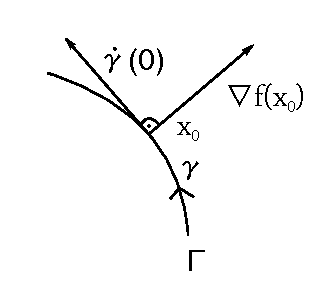
\includegraphics{img/tangential_vector.pdf}
      \caption{Tangential vector $\dot{\gamma}(0)$ on $\Gamma$ in $x_0$}
      \label{img:tan}
    \end{center}
  \end{figure}

  \begin{itemize}
    \item $\ang{\nabla f(x_0)}{\dot{\gamma}(0)} = 0$. Compare with Figure~\ref{img:tan}.
    \item $\nabla f(x_0)$ is normal to $\dot\gamma(0)$, hence normal to $\Gamma$.
  \end{itemize}
\end{rem}

\begin{theorem}
  Let $f: D \to \mathbb R$, $D \subset \mathbb R^m$ is open.
  Assume $\forall x \in D$ exist all partial derivatives
  $\partial_j f(x)$ for $j = 1, \ldots, m$ and every function $D \to \mathbb R$,
  $x \mapsto \partial_j f(x)$, is continuous.
  Then $f$ is differentiable in $D$.
\end{theorem}
\begin{proof}
\end{proof}

\meta{lecture}{9th of June 2016}{Wolfgang Ring}

Now consider the counterexample above:
\[
  f(\begin{bmatrix} x_1 \\ x_2 \end{bmatrix}) = \begin{cases}
    x_1 \frac{x_1 x_2}{x_1^2 + x_2^2}  & \text{for } \begin{bmatrix} x_1 \\ x_2 \end{bmatrix} \neq \begin{bmatrix} 0 \\ 0 \end{bmatrix} \\
    0                                & \text{for } \begin{bmatrix} x_1 \\ x_2 \end{bmatrix} = \begin{bmatrix} 0 \\ 0 \end{bmatrix}
  \end{cases}
\]

We know:
\[ \partial_1 f(\begin{bmatrix} 0 \\ 0 \end{bmatrix}) = \partial_2 f(\begin{bmatrix} 0 \\ 0 \end{bmatrix}) = 0 \]
Let $\begin{bmatrix} x_1 \\ x_2 \end{bmatrix} \neq \vec{0}$. Then it holds that
\begin{align*}
  \partial_1 f(\begin{bmatrix} x_1 \\ x_2 \end{bmatrix}) &= \frac{\overbrace{2 x_1 x_2}^{(x_1^2 + x_2^2)} - x_1^2 x_2 \cdot 2x_1}{(x_1^2 + x_2^2)^2} \\
  \partial_2 f(\begin{bmatrix} x_1 \\ x_2 \end{bmatrix}) &= \frac{x^2 (x_1^2 + x_2^2) - x_1^2 x_2 \cdot 2x_2}{(x_1^2 + x_2^2)^2} \\
  \partial_1 f(\begin{bmatrix} \varepsilon \\ \varepsilon \end{bmatrix}) &= \frac{2\varepsilon^2 \cdot 2\varepsilon^2 - \varepsilon^2 \varepsilon \cdot 2 \varepsilon}{(2\varepsilon^2)^2} \\
    &= \frac{2\varepsilon^4}{4\varepsilon^4} = \frac12 \\
  \partial_2 f(\begin{bmatrix} \varepsilon \\ \varepsilon \end{bmatrix}) &= \frac{\varepsilon^2 \cdot 2 \varepsilon^2 - \varepsilon^2 \varepsilon \cdot 2 \varepsilon}{(2\varepsilon^2)^2} = 0
\end{align*}

It holds that
\[ \lim_{\varepsilon\to0} \partial_2 f(\begin{bmatrix} \varepsilon \\ \varepsilon \end{bmatrix}) = 0 = \partial_2 f(\begin{bmatrix} 0 \\ 0 \end{bmatrix}) \]
but
\[ \lim_{\varepsilon\to0} \partial_1 f(\begin{bmatrix} \varepsilon \\ \varepsilon \end{bmatrix}) = \frac12 \neq \partial_1 f(\begin{bmatrix} 0 \\ 0 \end{bmatrix}) \]
Hence $\partial_1 f$ is non-continuous in $\begin{bmatrix} 0 \\ 0 \end{bmatrix}$.

\begin{proof}
  Idea: get close to $x_0 \in D$ along lines parallel to coordinate axes.
  Use Mean Value Theorem. Let $x_0 = \begin{bmatrix} x_0^1 \\ x_0^2 \\ \vdots \\ x_0^n \end{bmatrix} \in D$
  and $x = \begin{bmatrix} x^1 \\ \vdots \\ x^n \end{bmatrix} \in D$.
  We build path of $x_0$ to $x$ along coordinate lines.

  We let $\xi_0 = x_0$ and
  \[
  \xi_1 \coloneqq \begin{bmatrix} x^1 \\ x_0^2 \\ \vdots \\ x_0^n \end{bmatrix} \qquad
  \xi_2 \coloneqq \begin{bmatrix} x^1 \\ x^2 \\ x_0^3 \\ \vdots \\ x_0^n \end{bmatrix} \qquad
  \ldots \qquad
  \xi_k \coloneqq \begin{bmatrix} x^1 \\ \vdots \\ x^k \\ x_0^{k+1} \\ \vdots \\ x_0^n \end{bmatrix} \qquad
  \xi_n = X
  \]

  It holds that $\xi_k + (x^{k+1} - x_0^{k+1}) e_{k+1} = \xi_{k+1}$.
  \[ \varphi_k: (-a_k, 1 + a_k) \subseteq \mathbb R \to \mathbb R \qquad a_k > 0 \]
  \[ \varphi_k(t) = f(\xi_k + t(x^{k+1} - x_0^{k+1}) \cdot e_{k+1}) \]
  \[ \varphi_k(0) = f(\varphi_k) \qquad \varphi_k(1) = f(\xi_{k+1}) \]

  $\varphi$ is continuously differentiable on $(-a_k, 1 + a_k)$ because $\varphi_k = f \circ l_k$
  and $l_k(t) = \xi_k + t(x^{k+1} - x_0^{k+1}) e_{k+1}$. $f$ is (along $l_k$) continuously differentiable
  by precondition for continuity of the $(k+1)$-th partial derivative.
  \[ \varphi'_k(t) = \partial_{k+1} f(l_n(t)) \cdot (x^{k+1} - x_0^{k+1}) \]
\end{proof}

\begin{align*}
  &\lim_{h\to0} \frac1{h} \left(f(l_n(t+h)) - f(l_n(t))\right) \\
  &= \lim_{h\to0} \frac1{h} \left(f(\xi_k + \overbrace{(t+h)(x^{k+1} - x_0^{k+1})\cdot e_{k+1}}^{= v_k + h(x^{k+1} - x_0^{k+1}) e_{k+1}})\right) \\
  &- f\left(\xi_n + \overbrace{t(x^{k+1} - x_0^{k+1}) \cdot e_{k+1}}^{v_k}\right) \\
  &\overset{(*)}{=} \lim_{h\to0} \frac1{h} (-f(\xi_k + v_k) + f(\xi_k + h \cdot (x^{k+1} - x_0^{k+1}) e_{k+1})) \\
  &\overset{\text{claim}}{=} \partial_{k+1} f(\xi_k + v_k) \cdot (x^{k+1} - x_0^{k+1})
\end{align*}
This is true for $x^{k+1} = x_0^{k+1}$. For $x^{k+1} - x_0^{k+1} \neq 0$ it holds that
\begin{align*}
  (*) &= (x^{k+1} - x_0^{k+1}) \lim_{h\to0} \frac{1}{\underbrace{h(x^{k+1} - x_0^{k+1})}_{\tilde{h}}} \\
  &\cdot (-f(\xi_k + v_k) - f(\xi_k + v_k + \overbrace{h(x^{k+1} - x_0^{k+1})}^{\tilde{h}} \cdot e_{k+1}) \\
  &= (x^{k+1} - x_0^{k+1}) \cdot \underbrace{\lim_{\tilde{h}\to0} \left(-f(\xi_k + v_k) + f(\xi + v_k + \tilde{h} e_{k+1})\right)}_{\partial_{k+1} f(\xi_k + v_k)}
\end{align*}

Apply Mean Value Theorem to $\varphi_k$:
\[ \exists \tau_k \in (0,1): f(\xi_{k+1}) - f(\xi_k) = \varphi(1) - \varphi(0) \]
\[ = \varphi'(\tau_k) \cdot (1 - 0) = \partial_{k+1} f(\xi_k + \tau_k(x^{k+1} - x_0^{k+1}) \cdot e_{k+1}) \cdot (x^{k+1} - x_0^{k+1}) \]

Claim: $f$ is differentiable, hence
\[ Df(x_0) = \begin{bmatrix} \partial_1 f(x_0) & \ldots & \partial_n f(x_0) \end{bmatrix} \]
Show that,
\[ \frac{1}{\norm{x - x_0}} \norm{f(x) - f(x_0) - \begin{bmatrix} \partial_1 f(x_0) & \ldots & \partial_n f(x_0) \end{bmatrix} (x - x_0)} \to 0 \text{ for } x \to x_0 \]

\begin{align*}
  &\frac1{\norm{x - x_0}} \norm{\underbrace{f(x)}_{\xi_n} - \underbrace{f(x_0)}_{\xi_0} - \sum_{k=1}^n \partial_k f(x_0) (x^k - x_0^k)} \\
  &=\frac{1}{\norm{x - x_0}} \| \underbrace{f(\xi_n) - f(\xi_{n-1})}_{\varphi_{k-1}(1) - \varphi_{k-1}(0)} + f(\xi_{n-1}) - f(\xi_{n-2}) + \ldots + f(\xi_1) \\
  &\hspace{58pt}- f(\xi_1) - \sum_{k=1}^n \partial_k f(x_0) (x^k - x_0^k)\| \\
  &= \frac{1}{\norm{x - x_0}} \| \sum_{k=1}^n \partial_k f(\xi_{k-1} + \tau_{k-1} (x^k - x_0^k) \cdot e_k) (x^k - x_0^k) \\
  &\hspace{58pt}- \sum_{k=1}^n \partial_k f(x_0) (x^k - x_0^k) \| \\
  &\leq \frac{1}{\norm{x - x_0}} \cdot \sum_{k=1}^n \abs{x^k - x_0^k} \cdot \norm{\partial_k f(\xi_{k-1} + \tau_{k-1}(x^k - x_0^k) \cdot e_k) - \partial_k f(x_0)}
\end{align*}
It holds that $\abs{x^k - x_0^k} \leq \norm{x - x_0}$.
\[ \leq \sum_{k=1}^n \underbrace{\norm{\partial_k f(\xi_{k-1} + \tau_{k-1}(x^k - x_0) e_k) - \partial_k f(x_0)}}_{(**)} \]
Now let $\varepsilon > 0$ be arbitrary and $\delta$ sufficiently large such that
\[ \norm{\partial_k f(y) - \partial_k f(x_0)} < \frac{\varepsilon}{n} \]
if $\norm{y - x_0} < \delta$.

Now choose $\inorm{x - x_0} < \frac{\delta}{M}$ where $M$ will be defined later
and consider $\xi_{k-1} + \tau_{k-1} (x^k - x_0^k) \cdot e_k - x_0$,
\[
\begin{bmatrix} x^1 \\ x^2 \\ \vdots \\ x_0^k \\ x_0^{k+1} \end{bmatrix}
+ \tau_{n-1} \begin{bmatrix} 0 \\ \vdots \\ x^k - x_0^k \end{bmatrix}
- \begin{bmatrix} x_0^1 \\ \vdots \\ x_0^n \end{bmatrix}
\]
where $x^k - x_0^k$ can be found on the $k$-th index.
\[ = \begin{bmatrix} x^1 - x_0^1 \\ x^2 - x_0^2 \\ \vdots \\ \tau_{k-1}(x^k - x_0^k) \\ 0 \\ \vdots \\ 0 \end{bmatrix} \]

\[ \norm{\xi_{k-1} + \tau_{k-1} (x^k - x_0^k) e_k - x_0} \leq \sum_{j=1}^{k-1} \abs{x^j - x_0^j} \cdot \norm{e_j} + \tau_{k-1} \abs{x^k - x_0^k} \cdot \norm{e_k} \]
\[ \leq \underbrace{\max_{k=1,\ldots,n} \abs{x^j - x_0^j}}_{\underbrace{\inorm{x - x_0}}_{\delta / M}} \cdot \underbrace{\max_{l=1,\ldots,n} \norm{e_k}}_{M>0} < \delta \]
\[ \Rightarrow (**) = \norm{\partial_k f(\xi_{k-1} + \tau_{k-1}(x^k - x_0^k) e_k) \partial_k f(x_0)} < \frac\varepsilon{n} \]

If $\inorm{x - x_0} < \frac\delta{M}$, it holds that
\[ \frac{1}{\norm{x - x_0}} \norm{f(x) - f(x_0) - [\partial_1 f(x_0), \ldots, \partial_n f(x_0)](x - x_0)} < \varepsilon \]

\subsection{Generalization}

Let $f: D \subseteq \mathbb R^n \to \mathbb R^m$, $D \subseteq \mathbb R^n$ open.
Assume all partial derivatives $\partial_j f^i(x)$ exist and be continuous in $x$ in $D$ with $j = 1, \ldots, n$ and $j = 1, \ldots, m$. Then $f$ is differentiable in $D$ and it holds that
\[ Df(x) = \left(\partial_i f^j(x)\right)_{\substack{i=1,\ldots,m \\ j = 1,\ldots,n}} \]

\subsection{Maxima and Minima}
%
\index[English]{Relative maximum}
\index[English]{Relative minimum}
\index[English]{Local maximum}
\index[English]{Local minimum}
\index[English]{Strict local maximum}
\index[English]{Strict local minimum}
\index[German]{\foreignlanguage{ngerman}{Relatives Maximum}}
\index[German]{\foreignlanguage{ngerman}{Relatives Minimum}}
\index[German]{\foreignlanguage{ngerman}{Lokales Maximum}}
\index[German]{\foreignlanguage{ngerman}{Lokales Minimum}}
\index[German]{\foreignlanguage{ngerman}{Striktes lokales Maximum}}
\index[German]{\foreignlanguage{ngerman}{Striktes lokales Minimum}}
Let $D \subseteq \mathbb R^n$ and $f: D \to \mathbb R$. We call $x_0 \in D$
a \emph{relative maximum} (\emph{relative minimum}) or \emph{local maximum} (\emph{local minimum}) of $f$ if $\varepsilon > 0$ exists such that $\forall x \in B(x_0, \varepsilon) \cap D$ such that $f(x) \leq f(x_0)$ ($f(x) \geq f(x_0)$).
We call the maximum (minimum) \emph{strict}, if for $x \neq x_0$, the inequality holds strictly.

\subsection{Necessary optimality criterion}
%
\begin{theorem}[Necessary optimality criterion]
Let $D \subseteq \mathbb R^n$ open, let $x_0 \in D$ be a local maximum or a local minimum. Let $f$ be differentiable in $x_0$. Then for all $v \in \mathbb R^n \setminus \{\vec{0}\}$:
\[ df(x_0; v) = Df(x_0) \cdot v = 0 \]
Especially $Df(x_0) \cdot e_k = \partial_k f(x_0) = 0$ for $k = 1, \ldots, n$. Hence,
\[ Df(x_0) = \begin{bmatrix} 0 & 0 & \ldots & 0 \end{bmatrix}
\quad \text{ or equivalently } \quad
\nabla f(x_0) = \begin{bmatrix} 0 \\ 0 \\ \vdots \\ 0 \end{bmatrix} \]
\end{theorem}
%
\begin{proof}
  Let $l_{v,x_0}(t) = x_0 + t \cdot v$. If $x_0$ is a local maximum,
  it holds that
  \[ f(l_{v,x_0}(t)) \leq f(l_{v,x_0}(0)) = f(x_0) \]
  for sufficiently small $t$.
  So $f \circ l_{v,x_0}$ has a local maximum at $t = 0$.
  \[ (f \circ l_{v,x_0})'(0) = df(x_0; v) = 0 \]
  by necessary optimality criteria for functions in $\mathbb R$.
\end{proof}

\meta{lecture}{14th of June 2016}{Wolfgang Ring}

Recall: A set $X$ with a map $d: X \times X \to [0, \infty)$ is called \emph{metrical space} if
\begin{enumerate}
  \item $d(x, y) = 0 \Leftrightarrow x = y$
  \item $\forall x, y: d(x, y) = d(y, x)$
  \item $\forall x, y, z \in X: d(x, z) \leq d(x, y) + d(y, z)$
\end{enumerate}

Using metrics, we can define convergent sequences and Cauchy sequences.

$(x_n)_{n\in\mathbb N}$ is convergent with limit $x \in X$ if
\[
  \forall \varepsilon > 0 \exists N \in \mathbb N:
          [n \geq N \implies d(x_n, x) < \varepsilon]
\]
Cauchy sequence:
\[
\forall \varepsilon > 0 \exists N \in \mathbb N:
        [n,m \geq N \implies d(x_n, x_m) < \varepsilon]
\]

\begin{defi}
  A metric space $(X, d)$ is called \emph{complete}, if every Cauchy sequence in $X$
  is also a convergent sequence, hence has a limit.
\end{defi}

\begin{lemma}
  Every normed vector space $(V, \norm{.})$ induces also a metric space
  $d(v, w) = \norm{v - w}$.

  Let $V$ be complete and $A \subseteq V$ bounded. Then $A$ with metric
  $d(v,w) = \norm{v - w}$ is a complete metric space.
\end{lemma}

\begin{proof}[Metric properties of $d(v,w) = \norm{v - w}$]
  Let $A \subseteq V$ be bounded and let $(v_n)_{n \in \mathbb N}$ be a Cauchy
  sequence in $A$, hence $v_0 \in A \forall n \in \mathbb N$.
  Then $(v_n)_{n\in\mathbb N}$ is a Cauchy sequence in $V$.
  Because $V$ is complete, $\exists v \in V: v = \lim_{n\to\infty} v_n$.

  This likewise means that $v$ is a contact point of $A$.
  Because $A$ is bounded, it holds that $v \in A$ ($A = \overline{A}$).
  Hence $(v_n)_{n\in\mathbb N}$ has a limit point in $A$.
\end{proof}

\index[English]{Banach's fixed point theorem}
\index[German]{\foreignlanguage{ngerman}{Banach's Fixpunktsatz}}
\index[English]{Contraction}
\index[German]{\foreignlanguage{ngerman}{Kontraktion}}
\index[English]{Fixed point}
\index[German]{\foreignlanguage{ngerman}{Fixpunkt}}
\begin{theorem}[Banach's fixed point theorem]
  Let $X$ be a complete metrical space. $F: X \to X$ with property
  $\exists \sigma \in [0,1)$ such that $d(F(x), F(y)) \leq \sigma \cdot d(x,y)$
  (a derivative with this property is called \emph{contraction}).

  Then a uniquely defined point $\overline{x} \in X$ with $F(\overline{x}) = \overline{x}$. $\overline{x}$ is called \emph{fixed point} of $F$.
  \begin{figure}[!h]
    \begin{center}
      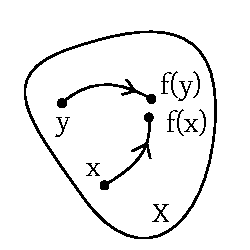
\includegraphics[width=0.2\textwidth]{img/banachs_fpt.pdf}
      \caption{Illustration for Banach's fixed point theorem}
    \end{center}
  \end{figure}
\end{theorem}

\begin{proof}
  Let $x_0 \in X$ be arbitrary.
  We define
  \[
  x_n = F(x_{n-1}) = \underbrace{F(F(\ldots(F(x_0))))}_{\text{nested } n \text{ times}}
  = F^{n}(x_0) = \underbrace{(F \circ F \circ F \ldots \circ F)}_{ \text{ times}}(x_0)
  \]
  for $n \in \mathbb N$ with $n \geq 1$.

  We show: $(x_n)_{n\in\mathbb N}$ is a Cauchy sequence. It holds that
  \[ d(\underbrace{x_n}_{=F(x_n)}, \ldots, \underbrace{x_n}_{F(x_{n-1})} \leq \sigma \cdot \underbrace{d(x_n, x_{n-1})}_{F(x_{n-1})} \]
  \[ \leq \vartheta^2 d(x_{n-1}, x_{n-2}) \leq \ldots \leq \vartheta^n d(x_1, x_0) \]

  Then for every $m,n \in \mathbb N$ with $m > n$.
  \begin{align*}
    d(x_m, x_n) &\leq d(x_m, x_{m-1}) + d(x_{m-1}, d_{m-2}) + \ldots + d(x_{n+1}, x_n) \\
    &\leq \vartheta^m d(x_1, x_0) + \vartheta^{m-1} \cdot d(x_1, x_0) + \ldots + \vartheta^{n+1} d(x_1, x_0) \\
    &= \vartheta^{n} \frac{1 - \vartheta^{m-n+1}}{1 - \vartheta} d(x_1, x_0) \\
    &< \vartheta^{n} \frac{1}{1 - \vartheta} d(x_1, x_0) \\
    &< \varepsilon \text{ if } \vartheta^n < \frac{\varepsilon (1 - \vartheta)}{d(x_1, x_0) + 1}
  \end{align*}
  Hence $\vartheta^n \to 0$ because $\vartheta < 1$ for sufficiently large $n$.

  So $(x_n)_{n \in \mathbb N}$ is a Cauchy sequence. Let $\overline{x}$ be the limit
  of this Cauchy sequence (completeness of $X$).

  $F$ is Lipschitz continuous, hence continuous in $X$.
  So it holds that $\lim_{n\to\infty} F(x_n) = F(\overline{x})$.
  \[ \lim_{n\to\infty} x_{n+1} = \overline{x} \]
  Followingly $\overline{x} = F(\overline{x}$, so $\overline{x}$ is a fixed point
  of $F$.

  It remains to show uniqueness:

  Let $\overline{y} = F(\overline{y})$. Assume $\overline{y} \neq \overline{x}$,
  hence $d(\overline{x}, \overline{y}) > 0$. Hence it holds that
  \[ d(\overline{x}, \overline{y}) = d(F(\overline{x}), F(\overline{y})) \]
  \[ \overset{\text{contraction}}{\leq} \vartheta d(\overline{x}, \overline{y}) \]
  \[ \implies 1 \leq \sigma \]
  This a contradiction.
\end{proof}

\index[English]{Local Inverse Map Theorem}
\index[German]{\foreignlanguage{ngerman}{Lokaler Umkehrsatz}}
\index[English]{Diffeomorphism}
\index[German]{\foreignlanguage{ngerman}{Diffeomorphismus}}
\begin{theorem}[Local Inverse Theorem, Theorem of the inverse map]
  Let $O \subseteq \mathbb R^n$ be open and let $f: O \to \mathbb R^m$ be
  continuously differentiable in $O$. Let $x_0 \in O$ such that
  $\underbrace{Df(x_0)}_{\mathbb R^{n\times n}}$  is regular (invertible).

  Then there exists an environment $U$ of $x_0$ such that $f: U \to f(U) \subseteq \mathbb R^m$ is bijective.

  Even more it holds that $f: U \to f(U)$ is a \emph{Diffeomorphism}.
  Hence $f$ is bijective and $f^{-1}: f(U) = V \to U$ is continuously differentiable.
  Furthermore it holds that
  \[ D(f^{-1})(\underbrace{y_0}_{f(x_0)}) = \left[Df(x_0)\right]^{-1} \]
\end{theorem}
\begin{proof}
  Consider $\tilde{f}(x) = f(x + x_0) - f(x_0)$.
  \[ \tilde{f}: O - x_0 = \set{z - x_0: z \in O} \to \mathbb R^n \]
  \[ \tilde{f}(0) = 0 \]
  \[ D\tilde{f}(0) = Df(x_0) \]
  It follows immediately that $\tilde{f}$ is a Diffeomorphism iff $f$ is a Diffeomorphism.

  Let $F: \tilde{O} \to \mathbb R^n$ with $F(x) = \underbrace{[Df(x_0)]^{-1}}_{\text{exists by hypothesis}} \cdot \tilde{f}(x)$. Then it holds that $F(0) = 0$.
  \[ DF(0) = [Df(x_0)]^{-1} \cdot \underbrace{D\tilde{f}(0)}_{Df(x_0)} = I \]
  So it holds that, $F$ is continuously differentiable in $\tilde{O}$ with $DF(0) = I$. We show: $F$ is a Diffeomorphism.

  We let $y \in \mathbb R^n$ such that,
  \[ \varphi_y(x) = y + x - F(x) \]
  Then it holds that $\varphi_y(x) = x \iff x = y + x - F(x) \iff y = F(x)$.
  Hence $x$ is the solution of $F(x) = y \iff x$ is fixed point of $\varphi_y$.

  $F$ is continuously differentiable.
  Because $F$ is continuously differentiable, it holds that $\varphi_y$ is continuously differentiable:
  \[ D\varphi_y(X) = I - DF(x) \]
  Because of continuous differentiability, $\underbrace{DF(x)}_{\mathbb R^{m\times n}}$ depends continuously on $x$.

  So, $\forall \varepsilon > 0 \exists \delta > 0:$
  \[ \norm{x - 0} < \delta \implies \underbrace{\norm{DF(x) - \underbrace{DF(0)}_{=I}}}_{\text{operator norm}} < \varepsilon \]
  Choose $r > 0$ such that
  \[ \norm{x} < 2r \implies \norm{DF(x) - I} < \frac12 \]
  and we choose $r$ sufficiently small such that $B(O,2r) \subseteq \tilde{O}$. This works only because $\tilde{O}$ is open.

  Let $x_1, x_2 \in B(O, 2r)$.
  \[ l_{x_1,x_2}: (-\varepsilon, 1 + \varepsilon) \to B(O, 2r) \]
  \[ l_{x_1,x_2}(t) = (1 - t) x_1 + t x_2 \]
  \[ l_{x_1,x_2}(0) = x_1 \qquad l_{x_1,x_2}(1) = x_2 \]

  Consider
  \[ \norm{\varphi_y(x_2) - \varphi_y(x_1)} = \norm{\varphi_y \circ l_{x_1,x_2}(1) - \varphi_y \circ l_{x_1,x_2}(0)} \]
  \[ = \norm{\int_0^1 \frac{d}{dt} [\varphi_y \circ l_{x_1,x_2}(t)] \, dt} \]
  \[ = \norm{\int_0^1 D\varphi_y(l_{x_1,x_2}(t)) \cdot (x_2 - x_1) \, dt} \]
  \[ \leq \int_0^1 \norm{D\varphi_y(l_{x_1,x_2}(t)) \cdot (x_2 - x_1)} \, dt \]
  \[ \leq \int_0^1 \norm{D\varphi_y(l_{x_1,x_2}(t))} \norm{x_2 - x_1} \, dt \]
  \[ = \int_0^1 \overbrace{\norm{I - DF(\underbrace{l_{x_1,x_2}(t)}_{\in B(O,2r)})}}^{\leq \frac12} \, dt \cdot \norm{x_2 - x_1} \]
  \[ \leq \frac12 \norm{x_1 - x_2} \]

  Hence $\varphi_y$ is a contraction with $\sigma = \frac12$.
  It remains to show that $\varphi_y: B(O,r) \to B(O,r)$ ($\varphi_y$ maps to itself) for sufficiently small $y$.

  Let $y \in B(O,r)$ and $x \in B(O, 2r)$. Then it holds that
  \[ \norm{\varphi_y(x)} \leq \underbrace{\norm{\varphi_y(x) - \varphi_y(0)}}_{\leq \frac12 \norm{x - 0} \text{ by contraction}} + \underbrace{\norm{\varphi_y(0)}}_{=\norm{y}} \]
  \[ \leq \frac12 \cdot 2r + r = 2r \]
  \[ \varphi_y(x) \in B(O, 2r) \subseteq B(O,2r) \]
  So for $y \in B(O,r)$ it holds tat
  \[ \varphi_y: \overline{B(O,2r)} \to \overline{B(y,2r)} \]
  Then by Banach's fixed point theorem, there exists some unique
  $x \in \overline{B(O,2r)}$ with $\varphi_y(x) = x$, hence $F(x) = y$.

  We show: $DF(x)$ is invertible for all $x \in U = F^{-1}(B(O,r)) \cap B(O,2n)$.

  We know:
  \[ \norm{v - DF(x) \cdot v} = \norm{(I - DF(x)) \cdot v} \]
  \[ \leq \norm{I - DF(x)} \cdot \norm{v} \leq \frac12 \norm{v}
  \qquad \forall x \in U \]
  Let $v \in \kernel{(I - DF(x))}$.
  Then it holds that
  \[ \norm{v} = \norm{v - DF(x) \cdot v + DF(x) \cdot v} \]
  \[ \leq \underbrace{\norm{v - DF(x) \cdot v}}_{\leq \frac12 \norm{v}} + \norm{DF(x) \cdot v}_{0} \]
  \[ \implies \frac12 \norm{v} \leq 0 \implies v = 0 \]
  For $x \in U$ it holds that $\kernel{DF(x)} = \set{0} \implies DF(x)$ is invertible.
\end{proof}

% FYI integral of a norm is smaller than the norm of an integral

\meta{lecture}{16th of June 2016}{Wolfgang Ring}

\begin{proof}[cont.]
  because (by $\norm{\varphi_y(x)} \leq 2r$, the conclusion using Banach's fixed point theorem)
  for the fixed point $x$ in $\varphi_y$, it holds that
  \[ \norm{x} = \norm{\varphi_y(x)} < 2r \]
  Hence for every $y \in B(O,r)$ there exists a unique $x \in B(O,2r)$ such that $F(x) = y$.

  Hence in $U = B(O,2r) \cap F^{-1}(B(O,r))$ the map $f$ is injective. So $F: U \to F(U) = B(O,r)$
  bijective. Furthermore $F^{-1}(B(O,r))$ is open\footnote{Preimages of open sets in continuous
  maps are also open. Will be shown later.}.
  Hence $U$ is open. Therefore $f$ (bijective backtransformation) bijective in some environment
  of $x_0$.

  We use a lemma, which is not proven here:
  \begin{lemma}
    Let $g: D \subseteq \mathbb R^n \to \mathbb R^n$ continuously differentiable in $D$.
    Let $g$ be bijective and $Dg(x)$ invertible for all $x \in D$.
    Then $g^{-1}: g(D) \to D$ is continuously differentiable in $g(D)$ and it holds that
    \[ Dg^{-1}(\underbrace{y}_{g(x)}) = \left[Dg(x)\right]^{-1} \]
  \end{lemma}
  The lemma is proven in Königsberger volume 2, 3rd edition, page 105.

  This implies that $F^{-1}$ is differentiable in $B(O,1)$ with given Jacobimatrix.
  Therefore also $f^{-1}$ is differentiable.
\end{proof}

\subsection{A theorem about implicit functions}
%
\begin{theorem}
  Let $U \subseteq \mathbb R^{n + m} = \mathbb R^n \times \mathbb R^m$ and let
  $f: U \to \mathbb R^m$ continuously differentiable.

  Notation: $(x,y) \in U$ with $x \in \mathbb R^n$ and $y \in \mathbb R^m$.
  For some $(x_0, y_0) \in U$ let it hold that $f(x_0, y_0) = \vec{0}$.

  Furthermore let
  \[
  Df(x_0, y_0) = \begin{bmatrix}
    \partial x_1 f^1 & \partial x_2 f^1 & \ldots & \partial x_n f^1 & \partial y_1 f^1 & \ldots & \partial y_m f^1 \\
    \partial x_1 f^2 & \partial x_2 f^2 & \ldots & \partial x_n f^2 & \partial y_1 f^2 & \ldots & \partial y_m f^2 \\
    \vdots           &                 & \ddots &                  &                 & \ddots & \vdots \\
    \partial x_1 f^m & \partial x_2 f^m & \ldots & \partial x_n f^m & \partial y_1 f^m & \ldots & \partial y_m f^m
    \end{bmatrix}
  \]
  The left half side of the matrix is $D_x f(x_0, y_0) \in \mathbb R^{m\times n}$ whereas the right half of the matrix
  is $D_yf(x_0, y_0) \in \mathbb R^{m\times m}$.

  Assumption:$D_y f(x_0, y_0)$ is invertible.

  Then there exists some environment $U'$ of $x_0$ in $\mathbb R^n$ and a continuously differentiable function
  $g: U' \to \mathbb R^m$ with $g(x_0) = y_0$ and $f(x, g(x)) = \vec{0} \in \mathbb R^m$.

  $y = g(x)$ solves the implicit equation $f(x,y) = 0$.
\end{theorem}

\begin{proof}
  Let $F(x,y) = \begin{bmatrix} x \\ f(x,y) \end{bmatrix} \in \mathbb R^{n + m}$. $F: U \to \mathbb R^{n + m}$.
  \[
    DF(x,y) = \begin{bmatrix}
      I & 0 \\
      D_x f(x,y) & D_y f(x,y)
    \end{bmatrix}
  \] \[
    DF(x_0, y_0) = \begin{bmatrix}
      I  & 0 \\
      D_x f(x_0, y_0) & D_y f(x_0, y_0)
    \end{bmatrix}
  \] \[
    \det(DF(x_0, y_0))
      = \det{I} \cdot \underbrace{\det{D_y f(x_0, y_0)}}_{\neq 0} \neq 0
  \]
  So $DF(x_0, y_0)$ is invertible.
  From the local invertibility theorem it follows that
  \[ \implies V \subset \mathbb R^{n+m}: V \text{ is open, environment of } (x_0, y_0) \]
  \[ F: V \to F(V) \]
  is a Diffeomorphism. Let $r, r' > 0$ such that
  \[ B(x_0, r) \times B(y_0, r') \subseteq V \]
  $U \times U' \coloneqq B(x_0, r) \times B(y_0, r')$ is an open ball in $\mathbb R^{n+m}$ with norm
  $\norm{(x,y)}_{\mathbb R^{n+m}} = \max\set{\norm{x}, \norm{y}}$ in $\mathbb R^{n+m}$.
  $V$ is open in regards of this norm.

  For all $(\xi, \eta) \in F(U \times U')$ there exists a unique $(x,y) \in U \times U'$
  with $(\xi, \eta)^t = F(x,y)$ (local invertibility).
  \[ \iff \xi = x \land \eta = f(x, y) \]
  $x$ and $y$ are uniquely defined by $(\xi, \eta)$.
  Now let
  \[
  \begin{bmatrix} x \\ y \end{bmatrix}
  = F^{-1}(\xi, \eta)
  = \begin{bmatrix}
    \xi \\ G(\xi, \eta)
  \end{bmatrix}
  \]
  We let $g(x) = G(x, \vec{0})$.
  Then it holds that
  \[
    \begin{bmatrix} x \\ 0 \end{bmatrix}
    = F(F^{-1}(x, \vec{0}))
    = F(x, \underbrace{g(x)}_{=G(x,0)})
    = \begin{bmatrix} x \\ f(x, g(x)) \end{bmatrix}
  \]
  So $\vec{0} = f(x, g(x))$.

  Continuous differentiability of $g(x) = G(x, 0)$
  follows from continuous differentiability of $G$
  (over $F^{-1}$) by the local invertibility theorem.
\end{proof}

\begin{ex}
  Consider $f(x,y) = x^2 y - x^3 y^2 - 2$.
  \begin{align*}
    f(-1, 1) &= 1 - (-1) - 2 = 0 \\
    \partial_x f(x,y) &= 2xy - 3 x^2 y^2 \\
    \partial_y f(x,y) &= x^2 - 2 x^3 y \\
    \partial_x f(-1,1) &= -5  \neq 0 \\
    \partial_y f(-1,1) &= 3   \neq 0
  \end{align*}
  Hence, equation
  \[ x^2 y - x^3 y^2 - 2 = 0 \]
  in environment $(-1, 1)$ can uniquely solve
  the problem with $x$ as well as $y$.
\end{ex}

\section{Higher partial derivatives}

Consider $f: D \to \mathbb R$ (we consider
$f: D \to \mathbb R^m$ component-wise).
Let $D \subseteq \mathbb R^n$ be open.
Let $f$ in $D$ be continuously differentiable,
hence $\partial x_j f(x)$ is a continuous function
in $D$. Assume $\partial x_j f$ is continuously
differentiable in $D$. Let $\partial x_i x_j f
\coloneqq \partial x_i (\partial x_j f)$.
Analogously for higher derivatives: If
$\partial x_{i_1} x_{i_2} x_{i_3} \ldots x_{i_n} f
= \partial x_{i_1} (\partial x_{i_2} (\ldots (\partial x_{i_n} f) \ldots))$
if $\partial x_{i_2} x_{i_3} \ldots x_{i_n} f$
is continuously differentiable.

\begin{ex}
  \[ f(x, y) = x^2 y - x^3 y^2 - 2 \]
  \begin{align*}
    \partial x f &= 2xy - 3x^2 y^2 \\
    \partial_y f &= x^2 - 2x^3 y \\
    \partial_{xx} f &= 2y - 6xy^2 \\
    \partial_{yx} f &= 2x - 6x^2y \\
    \partial_{xy} f &= 2x - 6x^2 y \\
    \partial_{yy} f &= 0 - 2x^3
  \end{align*}
  Apparently the 3 derivatives are equal,
  so the order of $x$ and $y$ does not seem to be relevant.
\end{ex}

\index[English]{Hesse matrix}
\index[German]{\foreignlanguage{ngerman}{Hesse Matrix}}
Especially for 2 derivatives.
\[
  D^2 f(x) = \begin{bmatrix}
    \partial x_1 x_2 f & \partial x_1 x_2 f & \ldots & \partial x_1 x_n f \\
    \partial x_2 x_1 f & \partial x_2 x_2 f & \ldots & \partial x_2 x_n f \\
    \vdots            & \ddots             & \ddots & \vdots \\
    \partial x_n x_1 f & \ldots            & \ldots & \partial x_1 x_n f
  \end{bmatrix}
  (x)
\]
$D^2 f(x)$ is called \emph{Hesse matrix} of $f$. Under general conditions
(see Theorem by Schwarz) $D^2 f(x)$ is symmetrical. Hence eigenvalues of
$D^2 f(x)$ are real and there exists some orthonormal basis of eigenvectors.

\index[English]{Saddle point}
\index[German]{\foreignlanguage{ngerman}{Sattelpunkt}}
\begin{theorem}[Sufficient optimality criterion]
  Let $f: D \to \mathbb R$ such that the partial derivatives up to second
  degree in $D$ exist and are continuous. Let $x_0 \in D$ such that $Df(x_0) = 0$
  (i.e. $\nabla f(x_0) = \begin{bmatrix} 0 \\ \vdots \\ 0 \end{bmatrix}$).
  If $D^2 f(x_0)$ is negative definite (i.e. all eigenvalues are negative)
  \[ \fun{v, D^2f(x_0) v} < 0 \qquad \forall v \neq 0 \]
  then $f$ in $x_0$ has a local maximum. If $D^2 f(x_0)$ is positive definite,
  then $f$ in $x_0$ has a local minimum. If $D^2 f(x_0)$ is indefinite,
  then $f$ in $x_0$ has \emph{no} local extremum.
  We say: $f$ in $x_0$ has a \emph{saddle point}.
\end{theorem}

\begin{proof}
  Will be given later.
\end{proof}

Existence of local or global maxima/minima is commonly shown by compactness.

\index[English]{Continuously differentiable $k$ times}
\index[German]{\foreignlanguage{ngerman}{$k$-mal stetig differenzierbar}}
\begin{defi}
  Let $f: D \to \mathbb R$. $D$ is open and all partial derivatives of $f$
  up to degree $k$ exist and are continuous in $D$.
  Then $f$ is called continuously differentiable $k$ times in $D$ and
  we let
  \[ \mathcal{C}^k(D) = \set{f: D \to \mathbb R:
    f \text{ is continuously differentiable } k \text{ times}}
  \]
  $\mathcal{C}^k(D)$ is a real vector space.
\end{defi}

\fbox{Hermann Amandus Schwarz (1843--1921)}
\begin{defi}
  Let $D \subseteq \mathbb R^n$ be open, $f \in \mathcal{C}^2(D)$. Then it holds
  that $\partial x_i x_j f = \partial x_j x_i f$ in $D$.
\end{defi}
\begin{proof}[Schwarz' Theorem, Symmetry of second derivatives]
  Let $x_0 \in D$ be arbitrary. Let $r > 0$ such that $B(x_0, r) \subseteq D$
  and let $h,k \in \mathbb R$ be sufficiently small such that
  $x_0 + he_i \in B(x_0, \frac r2) \iff \norm{h \cdot e_i} \leq \frac r2$
  and $x_0 + ke_j \in B(x, \frac r2) \iff \norm{k e_j} < \frac r2$.

  Then it holds that $x_0 + he_i + ke_j \in B(x_0, r) \iff \norm{he_i + ke_j} < r$
  follows immediately because $\norm{he_i + ke_j} \leq \norm{he_i} + \norm{ke_j} < \frac r2 + \frac r2$.
  \meta{lecture}{17th of June 2016}{Wolfgang Ring}

  Let $F(h,k) = f(x_0 + he_i + ke_j) - f(x_0 + he_i) - f(x_0 + ke_j) + f(x_0)$.
  Let $x_0$ and $k$ be fixed.
  \[ \varphi(\lambda) = f(x_0 + \lambda e_i + k e_j) - f(x_0 + \lambda e_i) \]
  \[ \varphi: I \to \mathbb R \qquad I = (-1,1) \]
  \begin{figure}[!h]
    \begin{center}
      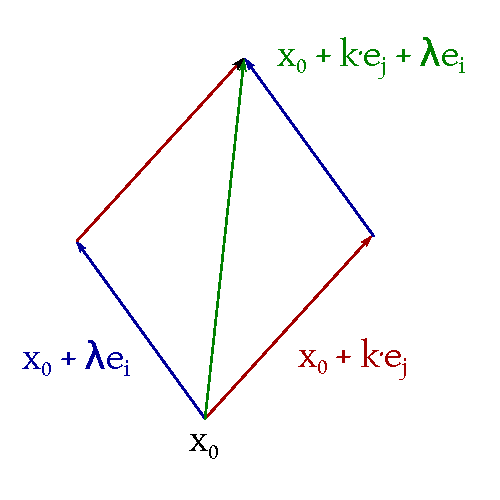
\includegraphics[width=0.4\textwidth]{img/schwarz-proof.pdf}
      \caption{$\varphi$ in the proof of Schwarz' Theorem}
      \label{img:schw-proof}
    \end{center}
  \end{figure}
  Compare with Figure~\ref{img:schw-proof}.

  \begin{align*}
    \varphi(0) &= f(x_0 + ke_j) - f(x_0) \\
    \varphi(h) &= f(x_0 + h\cdot e_i + k \cdot e_j) - f(x_0 + h \cdot e_i) \\
    \varphi(h) - \varphi(0) &= F(h,k)
  \end{align*}
  \[  \varphi: (-r, r) \to \mathbb R \]
  is continuously differentiable.
  The Intermediate Value Theorem gives us:
  \[ \exists \lambda \text{ with } \abs{\lambda} < \abs{h}: F(h,k) = \varphi(h) - \varphi(0) = h' \cdot \varphi'(\lambda) \]
  \[ = Df(x_0 + \lambda \cdot e_i + k \cdot e_j) \cdot e_i - Df(x_0 + \lambda e_i) \cdot e_i \]
  \[ = h \cdot \left[\partial x_i f(x_0 + \lambda \cdot e_i + k \cdot e_j) - \partial x_i f(x_0 + \lambda \cdot e_i)\right] \]
  Consider $\psi: (-r, r) \to \mathbb R$.
  \[ \psi(\mu) = \partial x_i f(x_0 + \lambda e_i + \mu e_j) \]
  $\psi$ is continuously differentiable, because $\partial x_i f$ is continuously differentiable.
  Hence
  \[
  F(h,k)
  = h \cdot [\psi(k) - \psi(0)]
  \underbrace{=}_{\text{IVT}, \abs{\mu} < \abs{\lambda}} h \cdot k \cdot \varphi'(\mu)
  = h \cdot k \partial x_i x_j f(x_0 + \lambda e_i + \mu e_j).
  \]
  Analogously: $\tilde{\varphi}(\mu) = f(x_0 + h \cdot e_i + \mu \cdot e_j) - f(x_0 + \mu \cdot e_j)$.

  Then it holds again that
  \[ F(h,k) = \tilde{\varphi}(k) - \tilde{\varphi}(0) \overbrace{=}^{\text{IVT}, \abs{\tilde{\mu}} < \abs{k}} k \cdot \tilde{\varphi}'(\mu) \]
  \[ = k \cdot \left[\partial x_j f(x_0 + he_i + \tilde{\mu} e_j) - \partial x_j f(x_0 + \tilde{\mu} \cdot e_j)\right] \]
  \[ \underbrace{=}_{\text{IVT}, \abs{\tilde{\lambda}} < \abs{h}} k \cdot h \cdot \left[\partial x_i x_j f(x_0 + \tilde{\lambda} e_i + \tilde{\mu} e_j)\right] \]
  \[ \implies h \cdot k \partial x_j \partial x_i f(x_0 + \lambda e_i + \mu e_j) \]
  \[ = k \cdot h \partial x_i \partial x_j f(x_0 + \tilde{\lambda} e_i + \tilde{\mu} e_j) \]
  \[
    \left.\begin{array}{c}
      \abs{\lambda} \abs{\tilde{\lambda}} < \abs{h} \\
      \abs{\mu} \abs{\tilde{\mu}} < \abs{k}
    \end{array}\right\}
    \text{ let $h, k$ go to zero (2nd derivatives are non-continuous}
  \]
  \[ \implies \partial x_j \partial x_i f(x_0) = \partial x_i \partial x_j f(x_0) \]
\end{proof}

\begin{ex}[Counterexamples]
  \[
  f(x_1, x_2) = \begin{cases}
    \frac{x_1 x_2 (x_1^2 - x_2^2)}{x_1^2 + x_2^2} & \text{ for } (x_1, x_2) \neq (0, 0) \\
    0 & \text{else}
  \end{cases}
  \]
  has second derivatives at every point. In $(0, 0)$ it holds that
  $\partial x_1 \partial x_2 f(0, 0) \neq \partial x_2 \partial x_1 f(0, 0)$.
\end{ex}

\begin{theorem}[Generalization of Schwarz' Theorem]
  Let $D \subseteq \mathbb R^n$ be open. $f \in \mathcal{C}^k(D)$.
  Then consider two variables you derive equal times with.
  Consider the corresponding resulting derivatives. They correspond
  (order of derivatives muss be smaller-equal $k$).

  For example:
  \[ \partial x_1 \partial x_3 \partial x_3 \partial x_1 = \partial x_1 \partial x_1 \partial x_3 \partial x_3 \]
\end{theorem}
\begin{proof}
  Can be done by complete induction.
\end{proof}

\index[English]{Multiindex}
\index[German]{\foreignlanguage{ngerman}{Multiindex}}
\begin{rem}[Multiindex notation]
  Let $I = (\alpha_1, \alpha_2, \ldots, \alpha_n) \in \mathbb N^n, \alpha_i \geq 0$.
  $I$ is called \emph{multiindex}. The number  $k = \abs{I} = \sum_{i=1}^n \alpha_i$
  is called \emph{order of $I$}.

  % TODO: normalize ``\partial smth'' to ``\partial_smth''
  Notation: $\partial_{x_l}^\alpha = \underbrace{\partial_{x_l} \partial_{x_l} \ldots \partial_{x_l}}_{\alpha \text{ times}}$ for $\alpha \in \mathbb N$.
  \[ \partial_{x_k}^0 f = f \quad\text{ and }\quad \partial_I f = \partial_{x_1}^{\alpha_1} \partial_{x_2}^{\alpha_2} \ldots \partial_{x_n}^{\alpha_n} \]

  Further notational remarks:
  \[ I! \coloneqq (\alpha_1!) (\alpha_2!) \ldots (\alpha_n!) = \prod_{i=1}^n (\alpha_i!) \]
  Let $x = (x_1, x_2, \ldots, x_n)^t$.
  Then we let $x^I = x_1^{\alpha_1} x_2^{\alpha_2} \ldots x_n^{\alpha_n} = \prod_{i=1}^n x_i^{\alpha_i}$.
\end{rem}

\begin{theorem}[Taylor's theorem]
  Let $f \in \mathcal{C}^{k+1}(D), D \subseteq \mathbb R^n$ be open.
  Let $x_0 \in D$ and $v$ sufficiently small such that the path between $x_0$ and $x_0 + v$ is entirely in $D$.

  Then some $w \in (0,1)$ exists such that
  \[ f(x_0 + v) = \underbrace{f(x_0) + \sum_{j=1}^k \sum_{i_1, i_2, \ldots, i_j = 1}^n \frac{1}{j!} \partial i_1, i_2, \ldots, i_j f(x_0) \cdot v_{i_1} \cdot v_{i_2} \cdot \ldots \cdot v_{i_m}}_{\text{Taylor polynomial of $f$ in $x_0$}}
  \] \[
  + \underbrace{\frac{1}{(j+1)!} \sum_{i_1, i_2, \ldots, i_{k+1}=1}^n \partial_{i_1, \ldots, i_{k+1}} f(x_0 + vw) \cdot v_{i_1} \cdot v_{i_2} \ldots v_{i_{k+1}}}_{R_{k+1}(f,v) \text{ as remaining term}}
  \]
\end{theorem}

Alternatively, we can write:
\[
  f(x_0 + v)
  = f(x_0) + \sum_{j=1}^k \sum_{\abs{I} = j} \frac{1}{I!} \partial_I f(x_0) \cdot v^I
  + \sum_{\abs{I}=k+1} \frac{1}{I!} \partial_I f(x_0 + vw) \cdot v^I
\]

\begin{proof}
  Let $B(x_0, r) \subseteq D$ and let $\abs{v} < r$. $\varphi: (-r, r) \to \mathbb R$.
  \[ \varphi(t) = f(x_0 + t \cdot v) = f \circ l_{x_0,v}(t) \]
  \[ l_{x_0,v}(t) = x_0 + t \cdot v \]
  Because $k$ is $(k+1)$ times continuously differentiable and the linear function
  $l_{x_0,v}$ can be differentiated arbitrary many times, so is $\varphi$ $k+1$ times differentiable.
  \[ \varphi'(t) = df(x_0 + t \cdot v) \cdot v = \sum_{i_1=1}^n \underbrace{\partial i_1 f(x_0 + tv)}_{\text{cont. diff. by $t$}} \cdot v_{i_1} \]
  \begin{align*}
    \varphi''(t) &= \sum_{i_1=1}^n \left(\sum_{i_2=1}^n \partial_{i_2} \partial_{i_1} f(x_0 + t \cdot v) \cdot v_{i_2}\right) \cdot v_{i_1} \\
    &= \sum_{i_1,i_2=1}^n \partial_{i_1,i_2} f(x_0 + t \cdot v) \cdot v_{i_1} v_{i_2}
  \end{align*}
  \[ \varphi^{(j)}(t) = \sum_{i_1,i_2,\ldots,i_j=0}^n \partial_{i_1,i_2,\ldots,i_j} f(x_0 + t v) \cdot v_{i_1} v_{i_2} \ldots v_{i_j} \]
\end{proof}

\begin{rem}[Taylor's theorem in the scalar case for $\varphi$]
  \[ \varphi(1) = \varphi(0) + \sum_{j=1}^k \frac{1}{j!} \varphi^{(j)}(0) + \frac{1}{(j+1)!} \varphi^{(j+1)}(v) \cdot 1^{j+1} \]
  with $v \in (0,1)$.
\end{rem}

\begin{rem}[Lagrange form of remaining term]
  For $\varphi$ and $\varphi^{(j)}$ we insert,
  \[ f(x_0 + v) = f(x_0) + \sum_{j=1}^k \frac{1}{j!} \sum_{i_1,i_2,\ldots,i_j=1}^n \partial_{i_1,i_2,\ldots,i_j} f(x_0) \cdot v_{i_1} \cdot v_{i_2} \cdot \ldots \cdot v_{i_j} \]
  \[ + \sum_{i_1,\ldots,i_{k+1}=1}^n \partial i_1 \ldots i_{k+1} f(x_0 + vw) \cdot v_{i_1} v_{i_2} \ldots v_{i_{k+1}} \]

  Taylor formula:
  \[ \partial_{i_1 i_2 \ldots i_j} f = \partial_{i'_1 i'_2 \ldots i'_j} f \]
  if $(i_1, i_2, \ldots, i_j) \in \mathbb N^j$ differs from $(i'_1, i'_2, \ldots, i'_j)$ only by its order.
  Let $I = (\alpha_1, \alpha_2, \ldots, \alpha_n) \in \mathbb N^n$ be a multiindex $I$ corresponding to
  derivative index
  \[ (\underbrace{1, 1, \ldots, 1}_{\alpha_1 \text{ times}}, \underbrace{2, 2, \ldots, 2}_{\alpha_2 \text{ times}}, \ldots, \underbrace{n, \ldots, n}_{\alpha_n \text{ times}}) \]
  \[ \abs{I} = j = \sum_{i=1}^n \alpha_i \qquad \tilde{I} \in \mathbb N^j \]
  How many permutations of $\tilde{I}$ are there in $\mathbb N$?

  Possibilities to distribute $\alpha_1$ ones over $j$ positions: $\binom{j}{\alpha_1}$.
  For every position of ones, $j - \alpha_1$ positions for twos remain.
  There exists $\binom{j-\alpha_1}{\alpha_2}$ possibilities to distribute the threes.
  $\binom{j-\alpha_1-\alpha_1}{\alpha_3}$, etc.

  Possibilities to distribute $\alpha_1$ ones, $\alpha_2$ twos, \dots, $\alpha_n$ n-es among $j$ positions:
  \[ A_I \coloneqq \binom{j}{\alpha_1} \binom{j-\alpha_1}{\alpha_2} \binom{j-\alpha_1-\alpha_2}{\alpha_3} \ldots \binom{j-\alpha_1-\alpha_2-\ldots-\alpha_{n-1}}{\alpha_n} \]
  is the number partial derivatives equivalent to $\partial_I$.
  \[ A_I = \frac{j!}{\alpha_1! (j-\alpha_1)!} \frac{(j-\alpha_1)!}{\alpha_2! (j - \alpha_1 - \alpha_2)!} \frac{(j-\alpha_1-\alpha_2)!}{\alpha_3!(j-\alpha_1 - \alpha_2 - \alpha_3)!} \]
  \[ \ldots \frac{(j-\alpha_1-\ldots-\alpha_{n-2})!}{\alpha_{n-1}!(j-\alpha_1-\ldots-\alpha_{n-1})!} \frac{(j-\alpha_1-\ldots-\alpha_{n-1})!}{\alpha_n! \underbrace{(j-\alpha_1-\ldots-\alpha_n)!}_{=0!=1}} \]
  Many terms cancel out. What remains is,
  \[ = \frac{j!}{\prod_{i=1}^n (\alpha_i)!} = \frac{j!}{I!} \]
  If $(i_1, \ldots, i_j)$ and $(i'_1, \ldots, i'_j)$ only distinguish by their order, then it holds that
  \[ v_{i_1} v_{i_2} \ldots v_{i_j} = v_{i'_1} \ldots v_{i'_j} = v^I \]
  Insert all these expressions in the Taylor formula and sum up equivalent expressions.
  \begin{align*}
    f(x_0 + v) &= f(x_0) + \sum_{j=1}^k \frac{1}{j!} \sum_{\abs{I}=j} \frac{j!}{I!} \partial_I f(x_0) \cdot v^I \\
    &+ \frac{1}{(k+1)!} \sum_{\card{I}=k+1} \frac{(k+1)!}{I!} \partial_I f(x_0 + vw) \cdot v^I
  \end{align*}
\end{rem}

\begin{ex}
  Let $f: \mathbb R^2 \to \mathbb R$, $f$ arbitrary often continuously differentiable.
  \begin{align*}
    f(x_0 + v)
    &= f(x_0) + \partial_1 f(x_0) \cdot v_1 + \partial_2 f(x_0) \cdot v_2 \\
    &+ \frac{1}{2! 0!} \cdot \partial_{(2,0)} f(x_0) \cdot v_1^2 \\
    &+ \frac{1}{1! 1!} \cdot \partial_{(1,1)} f(x_0) \cdot v_1 v_2
  \end{align*}
  The multiindex for $(1,1)$ is $(2,0)$.
  \[ + \frac{1}{0! 2!} \partial_{(0,2)} f(x_0) v_2^2 + \frac{1}{3! 0!} \partial_{(3,0)} f(x_0) v_1^3 + \frac{1}{2! 1!} \partial_{(2,1)} f(x_0) v_1^2 v_2 \]
  \[ + \frac{1}{1! 2!} \partial_{(1,2)} f(x_0) v_1 v_2^2 + \frac{1}{0! 3!} \partial_{(0,3)} f(x_0) v_2^3 + \ldots \]
  \[ = f(x_0) + \partial_1 f(x_0) v_1 + \partial_2 f(x_0) v_2 + \frac12 \partial_{11} f(x_0) v_1^2 \]
  \[ + \partial_{12} f(x_0) v_1 v_2 + \frac12 \partial_{22} f(x_0) v_2^2 + \frac16 \partial_{111} f(x_0) v_1^3 + \frac12 \partial_{112} f(x_0) v_1^2 v_2 \]
  \[ + \frac12 \partial_{122} f(x_0) v_1 v_2^2 + \frac16 \partial_{222} f(x_0) v_2^3 + \ldots \]
\end{ex}

\meta{lecture}{23rd of June 2016}{Wolfgang Ring}

Formula of 2nd degree: $\abs{I} = 2, j = 2$
\[ \sum_{i_1,i_2=1}^n \underbrace{\partial i_1 i_2 f(x_0)}_{[D_2 f(x_0)]_{i_1,i_2}} \cdot v_{i_1} v_{i_2} = \frac12 v^t \cdot D_2 f(x_0) \cdot v \]
where
\[ D_2f(x_0) =
\begin{bmatrix}
  \sum_{i_2=1}^n \partial_{1,i_2} f(x_0) \cdot v_{i_2} \\
  \sum_{i_2=1}^n \partial_{2,i_2} f(x_0) \cdot v_{i_2} \\
  \sum_{i_2=1}^n \partial_{n,i_2} f(x_0) \cdot v_{i_2}
\end{bmatrix}
\] \[
  v^t = (v_1, v_2, \ldots, v_n)
\]
Term of 2nd order in Taylor series:
\[ \frac12 v^t D_2 f(x_0) \cdot v \]

% TODO: normalize ``\partial_X'' (correct) versus ``\partial X'' (wrong)
\begin{theorem}[Taylor's Theorem, qualitative consideration]
  Let $f \in \mathcal{C}^K(D), x_0 \in D, D \subseteq \mathbb R^n$ open.
  Let $r>0$ such that $B(x_0, r) \subseteq D$ and let $\abs{v} < r$.
  Then it holds that
  \[ f(x_0 + v) = \sum_{j=0}^k \sum_{\abs{I} = j} \frac1{I!} \partial_I f(x_0) \cdot v^I + \underbrace{o(\norm{v}^k)}_{R_k(x_0;v)} \]
  where $o(\norm{v}^k) = g(v) \cdot \norm{v}^k$ with $\lim_{v\to0} g(v) = 0$.
\end{theorem}
\begin{proof}
  For this proof we use the Euclidean norm (then some estimates can be without constants).
  Because of equivalence of all norms, the proof follows for all norms.

  For Euclidean norm it holds that
  \[ \abs{v_i} = \sqrt{v_i^2} \leq \sqrt{\sum_{j=1}^n v_j^2} = \norm{v}_2 \]
  We use the Taylor formula with remaining term from before
  (we look at degree up to $k-1$).

  \[ f(x_0 + v) = \sum_{j=1}^{k-1} \sum_{\abs{I}=j} \frac{1}{\abs{I}!} \cdot \partial_I f(x_0) \cdot v^I + \sum_{\abs{I}=k} \frac{1}{I!} \cdot \partial_I f(x_0 + vw) v^I \]
  \[ + \sum_{\abs{I}=k} \frac{1}{I!} \partial_I f(x_0) v^I - \sum_{\abs{I}=k} \frac{1}{I!} \partial_I f(x_0) \cdot v^I \]
  \[ = \sum_{j=0}^k \sum_{\abs{I}=j} \frac{1}{I!} \partial_I f(x_0) v^I + \underbrace{\sum_{\abs{I}=k} \frac{1}{I!} \left[\partial_I f(x_0 + vw) - \partial_I f(x_0)\right] \cdot v^I}_{R_k(x_0;v)} \]

  \[ \abs{R_k(x_0, v)} \leq \sum_{\abs{I}=k} \frac{1}{I!} \abs{\partial_I f(x_0 + vw) - \partial_I f(x_0)} \cdot \underbrace{\abs{v_1^{i_1} v_2^{i_2} \ldots v_n^{i_n}}}_{\leq \norm{v}^{i_1} \cdot \norm{v}^{i_2} \ldots \norm{v}^{i_n}} \]
  \[ I = (i_1, i_2, \ldots, i_n) = \norm{v}^{i_1+\ldots+i_n} = \norm{v}^k \]
  and $D_I f(x_0 + vw) - D_I f(x_0) \to 0$ for $v\to 0$ because $f \in \mathcal{C}^k(D)$.

  So $\abs{R(x_0;v)} \leq \norm{v}^k \cdot \tilde{g}(v)$ with $\tilde{g}(v) \to 0$ for $v \to 0$, $\tilde{g}(v) \geq 0$.
  \[ \implies g(v) = \frac{\abs{R(x_0;v)}}{\norm{v}^k} \text{ for } v \neq \vec{0} \]
  \[ 0 \leq g(v) \leq \tilde{g}(v) \text{ and } \lim_{v\to0} g(v) = 0 \]
\end{proof}

\index[English]{Critical point}
\index[German]{\foreignlanguage{ngerman}{Kritischer Punkt}}
\begin{theorem}[Sufficient optimality criterion]
  Let $f: D \to \mathbb R$; $D \subseteq \mathbb R^n$ open. Let $x_0 \in D$ be a \emph{critical point} of $f$,
  hence $df(x_0) = \vec{0}$ or equivalently $\nabla f(x_0) = \vec{0}$.

  Assume
  \begin{enumerate}
    \item Let $D_2 f(x_0)$ be positive definite. Then $f$ has a strict local minimum in $x_0$.
    \item Let $D_2 f(x_0)$ be negative definite. Then $f$ has a strict local maximum in $x_0$.
    \item Let $D_2 f(x_0)$ be indefinite. Then $x_0$ is not an extremum. $x_0$ is called saddle point of $f$.
  \end{enumerate}
  $M$ is positive definite iff $v^t M v > 0 \quad \forall v \neq 0$.
\end{theorem}

\begin{figure}[!h]
  \begin{center}
    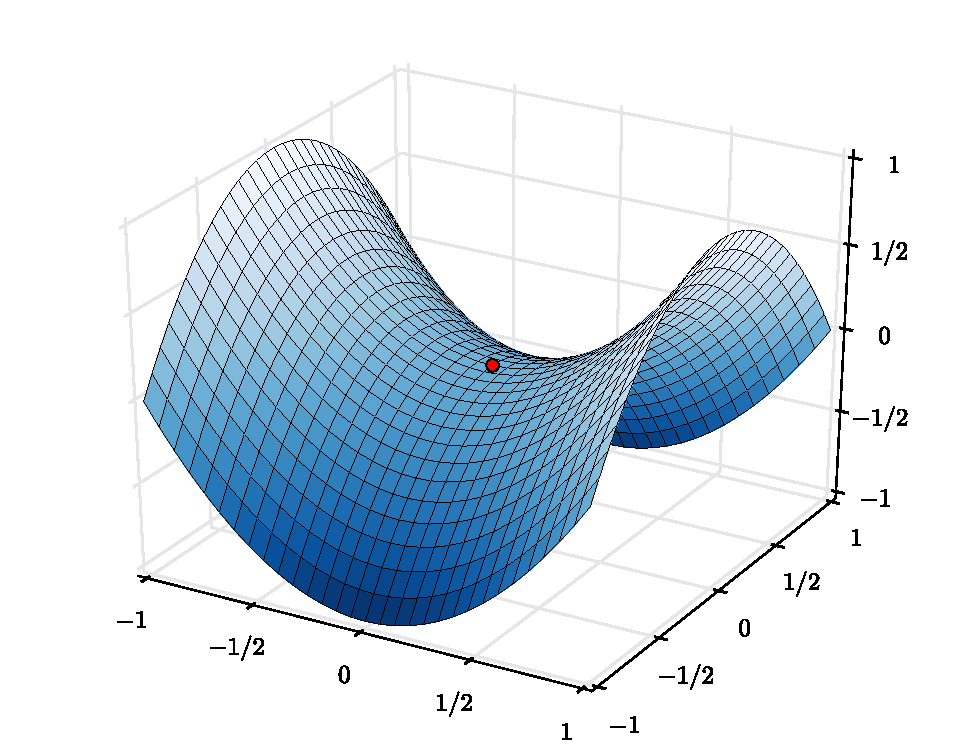
\includegraphics[width=0.4\textwidth]{img/saddle_point.pdf}
    \caption{Saddle point in $\mathbb R^2$, image by Nicoguaro}
    \label{img:saddlepoint}
  \end{center}
\end{figure}

\begin{proof}
  \begin{enumerate}
    \item
  Choose the Euclidean norm. Let $x_0$ be a critical point $D_2f(x_0)$ spd (symmetrically positive definite).
  Taylor:
  \[ f(x) = f(x_0) + \frac12 (x - x_0)^t D_2 f(x_0) (x - x_0) + o(\norm{x - x_0}) \]
  $D_2 f(x_0) = \vec{0}$ because $x_0$ is a critical point.
  \[ \implies f(x) - f(x_0) = \frac12 (x - x_0)^t D_2 f(x_0) (x - x_0) \norm{x - x_0}^2 \]
  because $\lim_{v\to 0} g(v) = 0$. Let
  \[ m = \min\set{\underbrace{\frac12 v^t D_2 f(x_0) v}_{>0 \quad \forall v \neq 0}: v \in \mathbb R^n, \norm{v} = 1} \]
  \[ S^{n-1} = \set{v \in \mathbb R^n: \norm{v} = 1} \qquad \text{$(n-1)$ sphere compact in $\mathbb R^n$} \]
  \[ v \mapsto \frac12 v^t D_2 f(x_0) v \]
  is continuous.
  So $m$ exists as minimum and $m > 0$.
  Let $\norm{x - x_0}$ be sufficiently small ($< \delta$) such that $0 \leq g(x - x_0) < \frac{m}{2}$.
  For $\norm{x - x_0} < \delta$ it holds that
  \[ f(x) - f(x_0) = \norm{x - x_0}^2 \left( \frac12
    \underbrace{\left(\frac{(x - x_0)^t}{\norm{x - x_0}}\right)^t}_{\eqqcolon v \in S^{n-1}}
    D_2 f(x_0) \frac{(x - x_0)}{\norm{x - x_0}} + g(x - x_0)
  \right)
  \]
  \[ \geq \norm{x - x_0}^2 (m - \frac{m}{2}) = \norm{x - x_0}^2 \frac{m}{2} > 0 \]
  for $x \neq x_0$ and $\norm{x - x_0} < \delta$.
  So $f(x) > f(x_0) \forall x\ \in B(x_0, \delta) \setminus \set{x_0}$.
  So $x_0$ is a strict minimum.

  \item analogously

  \item
  Let $D_2 f(x_0)$ be indefinite. Hence there exists eigenvalues $\lambda > 0$
  and $\mu < 0$ with eigenvectors $v,w$ such that
  \[ v^t \cdot D_2 f(x_0) \cdot v = v^t \cdot \lambda v = \lambda \norm{v}^2 > 0 \]
  and
  \[ w^t \cdot D_2 f(x_0) \cdot w = w^t \cdot \mu \cdot w = \mu \cdot \norm{w}^2 < 0 \]

  As in Taylor's formula:
  \[ \varphi(t) = f(x_0 + tv) \]
  \[ \varphi'(t) = \left\langle \nabla f(x_0 + tv); v\right\rangle \]
  \[ \varphi'(0) = 0 \text{ because } \nabla f(x_0) = \vec{0} \]
  \begin{align*}
    \varphi''(t) &= \sum_{i,j=1}^n \partial_{ij} f(x_0 + tv) \cdot v_i \cdot v_j \\
    &= \frac12 v^t D_2 f(x_0 + tv) \cdot v
    \varphi''(0) &= \frac12 v^t \cdot \lambda v > 0
  \end{align*}
  Hence $\varphi$ has a strict local minimum in $t=0$ (extreme value in 1 dimensional setting).
  \[ \varphi(t) = f(x_0 + tw) \]
  Analogously,
  \[ \psi'(0) = 0 \qquad \psi''(0) = \frac12 w^t \mu w < 0 \]
  hence $\psi$ has a strict local maximum in $t=0$.

  \begin{figure}[!h]
    \begin{center}
      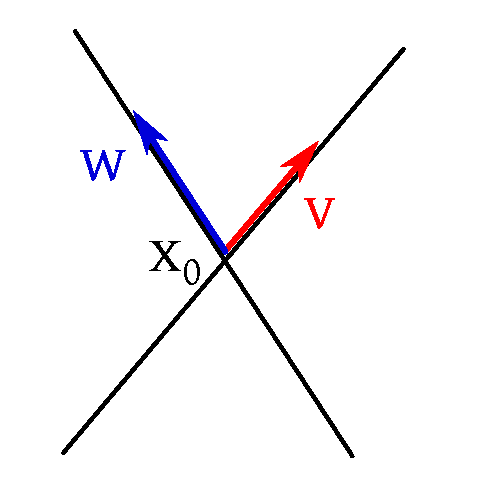
\includegraphics[width=0.2\textwidth]{img/min.pdf}
      \caption{
        $x_0$ is maximum by approximation along $w$.
        $x_0$ is minimum by approximation along $v$.
      }
      \label{img:min}
    \end{center}
  \end{figure}

  Compare with Figure~\ref{img:min}.
  Hence in every arbitrary small environment of $x_0$ there exists a point
  with larger function value ($x_0 + \varepsilon v$ for sufficiently small $\varepsilon$)
  and points with smaller function values ($x_0 + \varepsilon' w$ with $\varepsilon'$ sufficiently small).
  Hence $x_0$ is neither local maximum nor local minimum.
  \end{enumerate}
\end{proof}

\section{Additional results in topology}
\meta{lecture}{24th of June 2016}{Wolfgang Ring}
%
To discuss topology any further, we need additional results to fill some gaps
in our established theory. We look at those without context.

Reminder: $x_0 \in \mathbb R^n$. Then $U \subseteq \mathbb R^n$
with $x_0 \in U$ is called \emph{environment of $x_0$},
if $r>0$ exists such that $x_0 \in B(x_0,r) \subset U$.

$O \subseteq \mathbb R^n$ is open if and only if
$O$ is environment of every point $x \in O$.

\begin{lemma}
  $U$ is environment of $x_0 \in U$ if and only if
  there exists some open set in $\mathbb R^n$ with
  $x_0 \in O \subseteq U$.
\end{lemma}
\begin{proof}
  Let $U$ be an environment of $x_0$, then $B(x_0,r)
  = \set{x \in \mathbb R^n: \norm{x_0 - x} < r}$
  satisfies the properties of the open set $O$.
  Hence $B(x_0, r)$ is open in $\mathbb R^n$.
\end{proof}.

On the opposite, let $x_0 \in O \subseteq U$ with open $O$.
Then there exists, because $O$ is open, some $r > 0$:
$B(x_0,r) < O \implies B(x_0,r) \subseteq U$ because $O \subseteq U$.

Hence \enquote{environment} is a topological term
(hence can be defined with open sets only).

\index[English]{environments in $M$}
\index[German]{\foreignlanguage{ngerman}{Umgebung in $M$}}
\index[English]{environment relative to $M$}
\index[German]{\foreignlanguage{ngerman}{Umgebung relativ zu $M$}}
Let $M \subseteq \mathbb R^n$. We define environments and
open sets \emph{in M} (\emph{relative} to $M$).

\begin{defi}
  $O \subseteq M$ is called \emph{open} in $M$ if some open set
  $O^* \subseteq \mathbb R^n$ such that $O = M \cap O^*$.

  $U \subseteq M$ is called environment of $x_0$ \emph{in $M$} if
  some environment $U^*$ of $x_0$ in $\mathbb R^n$ exists such that
  $U = M \cap U^*$.
\end{defi}

\begin{ex}
  $M = Q \subseteq \mathbb R$.
  $O^* = (0,1)$ is open in $\mathbb R$.
  So $O = (0,1) \cap \mathbb Q = \set{g \in \mathbb Q: 0 < g < 1}$
  is open in $\mathbb Q$.

  But $O$ is \emph{not} an open set in $\mathbb R$ because in every
  interval $(q - \varepsilon, q + \varepsilon)$ for $q \in O$
  there are also irrational numbers.
\end{ex}

\begin{ex}
  Similarly, $M = [0,1]$. Then $\left(-\frac12, \frac12\right) \cap M = \left[0,\frac12\right)$
  is open in $M$, not open in $\mathbb R$.
\end{ex}

\begin{rem}
  Let $M \subseteq \mathbb R^n$ be open itself. Then $O \subseteq M$ is open in $M$
  if and only if $O$ is open.
\end{rem}
\begin{proof}
  Let $O = M \cap O^*$ be open in $M$ where $M$ and $O^*$ are open.
  Then $O$ is open in $\mathbb R^n$ as intersection of finitely many sets.

  On the opposite: Let $O \subseteq M$ be open in $\mathbb R^n$ itself.
  Then $O = M \cap O \implies O$ is open in $M$.
\end{proof}

\index[English]{Topology}
\index[German]{\foreignlanguage{ngerman}{Topologie}}
\index[English]{Relative topology}
\index[German]{\foreignlanguage{ngerman}{Relativtopologie}}
\begin{defi}
  Let $X$ be a set. $\tau \subseteq \mathcal{P}(X)$.
  Let $\tau$ satisfy properties:
  \begin{enumerate}
  \item $\psi \in \tau, x \in \tau$.
  \item Let $I$ be an index set and for every $i \in I$ let $O_i \in \tau$.
    Then it holds that $\bigcup_{i\in I} O_i \in \tau$.
  \item Let $O_1, \ldots, O_k \in \tau$, $k \in \mathbb N$.
    Then it holds that $\bigcap_{i=1}^k O_i \in \tau$.
  \end{enumerate}

  Then $\tau$ is called \emph{topology} in $X$. Elements $O$ of $\tau$ are called \emph{open sets}.

  Remark: $\set{O \subseteq \mathbb R^n: O \text{ is open}}$ is an topology in $\mathbb R^n$.
  Let $M \subseteq \mathbb R^n$. Then $\tau_M \coloneqq \set{O \subseteq M: O \text{ is open in } M}$
  is also a topology in $M$. $\tau_M$ is called \emph{relative topology} of $M$ in regards of $\mathbb R^n$.
\end{defi}

\begin{lemma}
  Let $M \subseteq \mathbb R^n$, $f: M \to \mathbb R^m$ and $x_0 \in M$.
  Then $f$ is continuous in $x_0$ iff for every environment $V$ of $y_0 = f(x_0)$ in $\mathbb R$
  it holds that $U = f^{-1}(V)$ is an environment of $x_0$ in $M$.

  $f: M \to \mathbb R^m$ is continuous in $M$ iff for every open set $O \subseteq \mathbb R^m$
  it holds that $f^{-1}(O)$ is open in $M$.
\end{lemma}

\begin{proof}
  First part:

  Let $\varepsilon > 0$ be arbitrary. Assume the preimages of environments of $y_0 = f(x_0)$
  are environments of $x_0$.
  Now let $V = B(y_0,\varepsilon)$ be an environment of $y_0$.
  Let
  \[ U = f^{-1}(V) = \set{x \in M: f(x) \in V} = \set{x \in M: \underbrace{\norm{f(x) - f(x_0)} < \varepsilon}_{\iff f(x) \in B(y_0,\varepsilon) = V}} \]
  By assumption $U$ is the environment of $x_0$ \emph{in $M$}.
  
  Hence $\exists \delta > 0: B(x_0, \delta) \cap M \subset U$.
  So for every $x \in B(x_0,\delta) \cap M$ it holds that
  $x \in U = f^{-1}(V)$ or equivalently $f(x) \in V$,
  hence $\norm{f(x) - f(x_0)} < \varepsilon$.

  We rewrite the implication of the last paragraph:
  $\forall x \in M$ with $\norm{x - x_0} < \delta$ it holds that
  $\norm{f(x) - f(x_0)} < \varepsilon$.
  Hence $f$ is continuous in $x_0$.

  On the opposite, let $f$ be continuous in $x_0$ and $V \subseteq \mathbb R^n$
  an arbitrary environment of $y_0 = f(x_0)$.
  Hence $\exists \varepsilon > 0: y_0 \in B(y_0, \varepsilon) \subseteq V$.
  Continuity implies $\exists \delta > 0: \forall x \in B(x_0,\delta) \cap M$
  it holds that $\norm{f(x) - f(x_0)} < \varepsilon$ with $f(x_0) = y_0$.
  Hence for these $x$ it holds that $f(x) \in B(y_0,\varepsilon) \subseteq V$.

  Equivalently $x \in f^{-1}(V)$.
  So it holds that $B(x_0,\delta) \cap M \subseteq f^{-1}(V)$.
  Then $f^{-1}(V)$ is environment of $x_0$ \emph{in $M$}.

  Second part:

  Let $f: M \to \mathbb R^m$ be continuous in every point of $M$.
  Let $O \subseteq \mathbb R^m$ be open. Then $O$ is environment of
  every point $y$ in $O$. Let $\tilde{O} = f^{-1}(O)$.
  If $\tilde{O} = \emptyset$, nothing has to be proven, because $\emptyset$ is open.
  Let $x \in \tilde{O}$ be arbitrary. Then it holds that $f(x) \in O$.
  Hence $O$ is environment of $y = f(x)$.

  By part 1, it holds that $\tilde{O}$ is environment of $x$.
  Hence $\tilde{O}$ is environment of every point $x \in \tilde{O}$,
  so $\tilde{O}$ is open in $M$.

  Now it remains to prove the other direction.
  
  On the opopsite, let the preimages of open sets be open and $x_0 \in M$ is arbitrary.
  Consider $y_0 = f(x_0) \in B(y_0,\varepsilon) \subseteq V$, hence $V$ is an
  arbitrary environment of $y_0$. Then it holds that $f^{-1}(B(y_0,\varepsilon))$
  is open in $M$. Furthermore it holds that
  \[ x_0 \in f^{-1}(B(y_0,\varepsilon)) \]
  Because $B(y_0,\varepsilon) \subseteq V$,
  \[ f^{-1}(B(y_0,\varepsilon)) \subseteq f^{-1}(V) \]
  where $f^{-1}(B(y_0,\varepsilon))$ is a relative open set, which contains $x_0$,
  so $f^{-1}(V)$ is an environment of $x_0$. By part1 is $f$ continuous in every point
  $x_0 \in M$.
\end{proof}

\section{Differentiability of linear and affine maps}
%
Let $A \in \mathbb R^{m\times n}$ and $f(x) = Ax + b$ ($b \in \mathbb R^m$).
$f: \mathbb R^n \to \mathbb R^m$. Because
\[ \norm{f(x) - f(y)} = \norm{Ax - Ay} \leq \norm{A} \cdot \norm{x - y} \]
Hence $f$ is Lipschitz continuous with constant $L = \norm{A}$.
$f$ is differentiable in every point $x \in \mathbb R^n$.
\[ \norm{f(x+h) - f(x) - Df(x) \cdot h} \]
We try $Df(x) = A$.
\[ = \norm{A (x + h) + b - Ax - b - A \cdot h} \]
\[ = \norm{\vec{0}} = 0 = O(\norm{H}) \]
So every affine function $f(x) = Ax + b$ is differentiable in $\mathbb R^n$
and it holds that $Df(x) = A$.

\meta{lecture}{28th of June 2016}{Wolfgang Ring}
\begin{lemma}
  Let $(X, d_X)$ and $(Y, d_Y)$ be metric spaces. Then by
  \[ d((x_1, y_1), (x_2, y_2)) = \max\set{d_X(x_1, x_2), d_Y(y_1, y_2)} \]
  with $(x_1, y_1), (x_2, y_2) \in X \times Y$ also $X \times Y$ is also
  a metric space.
\end{lemma}
\begin{proof}
  Symmetry follows by triangle inequality.
  Left as an exercise to the reader.
\end{proof}

\index[English]{Open cover}
\index[German]{\foreignlanguage{ngerman}{Offene Überdeckung}}
\index[English]{Partial open cover}
\index[German]{\foreignlanguage{ngerman}{Offene Teilüberdeckung}}
\begin{defi}
  Let $(K, \tau)$ be a topological space.
  Let $T \subseteq \mathbb{P}(X)$ be a topological space.
  We call $\set{U_i: i \in I}$ with $I$ as index set
  an \emph{open cover of $K$} if $U_1 \in \tau$ for all $i \in I$
  and $K \subseteq \bigcup_{i \in I} U_i$.

  The topological space $K$ is called compact if for every
  open cover $(U_i)_{i \in I}$ a finite index set
  $\set{i_1, i_2, \ldots, i_N} \subseteq I$ exists, such that
  \[ K \subseteq \bigcup_{j=1}^N U_{i_j} \]
  $(U_{i_j})_{j=1}^N$ is called \emph{finite partial cover} of $(U_i)_{i \in I}$.
\end{defi}

\index[English]{Sequence-compact space}
\index[German]{\foreignlanguage{ngerman}{Folgenkompakter Raum}}
\begin{defi}
  A metric space $K$ is called \emph{sequence-compact}
  if every sequence $(x_n)_{n \in \mathbb N}$ in $K$ has a convergent subsequence.
\end{defi}

\begin{theorem}
  Let $(K,d)$ be a compact metric spac.e Then $K$ is also
  sequence-compact.

  In other words:
  \begin{center} \enquote{Topologically compact implies sequence compact.} \end{center}
\end{theorem}
\begin{proof}
  Let $K$ be cover-compact.
  Let $(x_n)_{n \in \mathbb N}$ be an arbitrary sequence in $K$.
  % TODO: limit point / Haeufungspunkt is actually \omega-accumulating point
  Show that $(x_n)_{n \in \mathbb N}$ has a limit point (specifically: accumulating point).

  Assume $(x_n)_{n \in \mathbb N}$ does not have a limit point.
  $\forall y \in K \exists r_y > 0: B(y, r_y)$ contains only finitely many elements of the sequence.
  $B(y, r_y)$ is open.
  $(B(y, r_y))_{y \in K}$ is an open cover of $K$. Let $(B(y_i, r_{y_i}))_{i=1}^N$ a finite partial cover.
  The cover properties imply that $\forall n \in \mathbb N \exists i \in \set{1,\ldots,N}: x_n \in B(y_i, r_{y_i})$.
  On the other hand, every $B(y_i, r_{y_i})$ contains only finitely many sequence elements, hence
  $\bigcup_{i=1}^N B(y_i, r_{y_i})$ contains only finitely many sequence elements.

  This contradicts with statement that $\bigcup_{i=1}^N B(y_i, r_{y_i})$ contains all sequence elements.
\end{proof}

We also want to prove the opposite direction:
Sequence compact implies (topologically) compact.

\begin{lemma}
  Let $(K, d)$ be a sequence-compact metric space and let $(U_i)_{i \in I}$ be an open cover of $K$.
  Then there exists some $\delta > 0$ such that $\forall x \in K \exists i \in I$ with
  $B(x,\delta) \subseteq U_i$.
\end{lemma}
\begin{proof}
  Assume the statement does not hold. Then for every $\delta_n = \frac1n$ there exists
  some corresponding $x_n \in K$ such that $\forall i \in I: B(x_n, \delta_n) \not\subseteq U_i$.

  Due to sequence-compactness, $(x_n)_{n \in \mathbb N}$ is a convergent subsequence
  $(x_{n_k})_{n \in \mathbb N}$ with $x = \lim_{k\to\infty} x_{n_k}$.
  Because $(U_i)_{i \in I}$ cover $K$, there exists $i_x \in I$ such that $x \in U_{i_x}$
  where $U_{i_x}$ is open.
  So it holds that: $\varepsilon > 0: B(x, \varepsilon) \subseteq U_{i_k}$.
  Now let $n$ be sufficiently large such that $\delta_{n_k} = \frac{1}{n_k} < \frac{\varepsilon}{2}$
  and $d(x_{n_k}, x) < \frac{\varepsilon}{2}$.

  Let $y \in B(x_{n_{k_1}}, \delta_{n_k})$.
  \[ d(y, x) \leq f(y, x_{n_k}) + \underbrace{d(x_{n_k}, x)}_{< \frac\varepsilon2} < \varepsilon \]
  $f(y, x_{n_k})$ because $y \in B(x_{n_k}, \delta_{n_k})$ and $\delta_{n_k} < \frac{\varepsilon}{2}$.
  So it holds that $B(x_{n_k}, \delta_{n_k}) \subseteq B(x, \varepsilon) \subseteq U_{i_x}$.
  This is a contradiction to propery of $x_n - s$.
\end{proof}

\begin{theorem}
  Let $(K,d)$ be a sequence-compact topological space.
  Then $K$ is complete and compact.
\end{theorem}
\begin{proof}
  First we prove completeness.

  Let $(x_n)_{n \in \mathbb N}$ be a Cauchy sequence.
  Let $(x_{n_k})_{n \in \mathbb N}$ be a convergent subsequence with limit $x$.
  Then $x$ is also a limit of $(x_n)_{n \in \mathbb N}$.

  Reason: Let $\varepsilon > 0$ be arbitrary. Choose $N$ such that $n,m \geq N$.
  Then $d(x_n, x_m) < \frac{\varepsilon}{2}$. Choose $n_k \in \mathbb N$ such that
  $n_k \geq N$ such that $d(x_{n_k}, x) < \frac{\varepsilon}{2}$. Then for $n \geq N$
  it holds that
  \[ d(x_n, x) \leq d(x_n, x_{n_k}) + d(x_{n_k}, x) < \frac\varepsilon2 + \frac\varepsilon2 = \varepsilon \]
  So it holds that $x = \lim_{n\to\infty} x_n$.

  We show compactness.
  Sequence-compactness implies compactness.

  Let $(U_i)_{i \in I}$ be an open cover of $K$. Let $\delta > 0$
  as in the previous lemma. Hence $\forall x \in K \in i(x) \in I$ with
  $B(x, \delta) \subseteq U_{i(x)}$.

  We show:
  There are finitely many points $\set{y_1, y_2, \ldots, y_N}$ such that
  \[ K \subseteq \bigcup_{j=1}^N B(y_j, \delta) \subseteq \bigcup_{j=1}^N U_{i(y_j)} \]
  Then we have built a finite partial cover.

  We prove this by contradiction.
  Assume it does not hold. We construct $(y_i)_{i \in \mathbb N}$ inductively.
  Let $y_1 \in K$ be arbitrary. Then $K \subseteq B(y_0, \delta)$.
  Let $\set{y_1, \ldots, y_m}$ be already constructed.
  \[ K \not\subseteq \bigcup_{j=1}^m B(y_j, \delta) \]
  So there exists $y_{m+1} \in K \setminus \bigcup_{j=1}^m B(y_j, \delta)$,
  hence $y_{m+1} \not\in B(y_j, \delta)$ for $j = 1, \ldots, m$, hence
  $d(y_j, y_{m+1} > \delta$.

  Consider $(y_j)_{j \in \mathbb N}$. For $j \neq l$ it holds that
  $d(y_j, y_i) > \delta$. But $(y_j)_{j \in \mathbb N}$ is not a Cauchy
  sequence. Then $(y_j)_{j \in \mathbb N}$ also has no convergent subsequence,
  because every convergent subsequence must have the Cauchy property.
  This contradicts with sequence-compactness.

  So the proof is given and $\left(U_{i(y_j)}\right)_{j=1}^N$ is a finite partial cover of $K$.
\end{proof}

\index[German]{\foreignlanguage{ngerman}{Totalbeschränktheit}}
\index[English]{\foreignlanguage{english}{Total boundedness of $K$}}
\begin{defi}
  $K$ has the property
  \[ \forall \delta > 0 \exists \set{y_1, \ldots, y_N}: (N = N(\delta)) \]
  such that $K \subseteq \bigcup_{i=1}^N B(y_i, \delta)$.
  This property is called \emph{total boundedness of $K$}.
  ($K$ must not be compact and can be an arbitrary metric space)
\end{defi}

\begin{cor}
  \begin{center} compact $\iff$ complete and totally bounded \end{center}
\end{cor}

\subsection{Exchange theorems}

\begin{theorem}[Tube lemma]
  \label{tube-lemma}
  Let $X$ be an arbitrary metric space.
  Let $K$ be a compact metric space.
  Let $x_0 \in X$.

  We call set $\set{x_0} \times K$ the preimage (dt. Faser) over $x_0$ in $X \times K$.
  Compare with Figure~$\ref{img:faser}$.
  \begin{figure}[!h]
    \begin{center}
      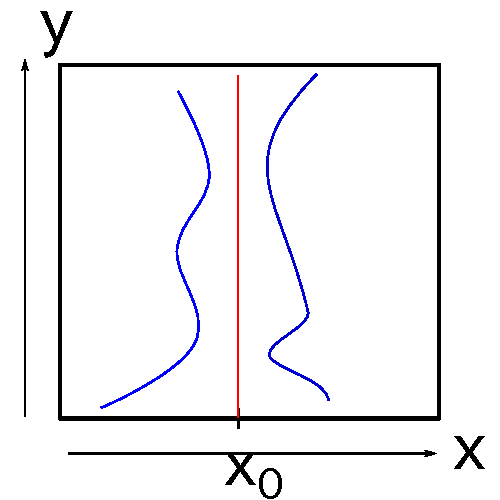
\includegraphics{img/faser.pdf}
      \caption{Faser over $x_0$ in $X \times K$}
      \label{img:faser}
    \end{center}
  \end{figure}

  Let $W \subset X \times K$ be open and $\set{x_0} \times K \subseteq W$.
  Then there exists some environment $U$ of $x_0$ in $X$ such that
  \[ \set{x_0} \times K \subseteq U \times K \subseteq W. \]

  A counterexample is given with $y = \frac{1}{\abs{x}}$ and $y = -\frac{1}{\abs{x}}$.
  \begin{figure}[!h]
    \begin{center}
      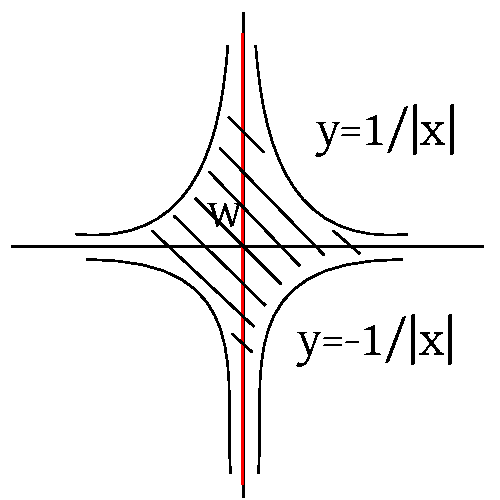
\includegraphics[width=0.4\textwidth]{img/counterexample.pdf}
      \caption{The counterexample}
      \label{img:counterexample}
    \end{center}
  \end{figure}
\end{theorem}
\begin{proof}
  Let $(x_0, y) \in \set{x_0} \times K \subset W$ because $W$ is open,
  there exists $B((x_0, y), r_y) \subseteq W$ with $r_y > 0$.

  \begin{align*}
    B((x_0, y), r_y) &= \set{(x,z): \max\set{d_X(x_0, x), d_K(y,z)} < r_y} \\
    &= \set{(x,z): d_X(x_0,x) < r_y \land d_K(y,z) < r_y} \\
    &= B_X(x_0, r_y) \times B_K(y, r_y)
  \end{align*}
  For $y \in K$, let $B_K(y, r_y)$ chosen as above. $\left(B_K(y, r_y)\right)_{y \in K}$ cover $K$.
  Because $K$ is compact, we choose a finite partial cover.
  Let $(B_k(y_i, r_{y_i}))_{i=1}^N$ be a finite partial cover.
  Then it holds that
  \[ \delta = \min\set{r_{y_i}: i = 1, \ldots, N} > 0 \]
  \[ \bigcup_{i=1}^N B_X(x_0, \delta) \times B_K(y_i, r_{y_i}) \subseteq \bigcup_{i=1}^N B_X(x_0, r_{y_i}) \times B(y_i, r_{y_i}) \subseteq W \]
  where $B_k(y_i, r_{y_i})$ cover $K$.
  \[ \bigcup_{i=1}^N \set{x_0} \times B(y_i, r_{y_i}) \subseteq \bigcup_{i=1}^N B_x(x_0, \delta) \times B(y_i, r_{y_i}) \]
  where $\bigcup_{i=1}^N \set{x_0} \times B(y_i, r_{y_i}) = \set{x_0} \times \bigcup_{i=1}^N B(y_i, r_{y_i}) = \set{x_0} \times K$.

  \begin{align*}
    \set{x_0} \times K \subseteq B_X(x_0, \delta) \times K
    &= B_X(x_0, \delta) \times \bigcup_{i=1}^N B(y_i, r_{y_i}) \\
    &= \bigcup_{i=1}^N \left(B_X(x_0, \delta) \times B(y_i, r_{y_i})\right) \subseteq W
  \end{align*}
\end{proof}

\begin{cor}
  Let $K, L$ be compact metric spaces. Then $K \times L$ are also compact.
\end{cor}
\begin{proof}
  Let $(W_i)_{i \in I}$ be an open cover of $K \times L$.

  Let $\set{x} \times L \subseteq K \times L$.
  Then there exists $\forall (x,y) \in F_y$ some $W_{i(y)}$ with $i(y) \in I$
  such that $(x,y) \in W_{i(y)}$ where $W_{i(y)}$ is open. Hence $\exists U_{i(y)}$
  % TODO: normalize {environment, neighborhood} to neighborhood
  and $V_{i(y)}$ as open neighborhood of $x$ in $K$ or equivalently
  of $y$ in $L$ such that $(x,y) \in U_{i(y)} \times V_{i(y)} \subseteq W_{i(y)}$.
  So for $x \in K$ it is fixed that the set system $(V_{i(y)})_{y \in L}$ is an open
  cover of $L$. Because $L$ is compact, there exists $i(y_1), \ldots, i(y_M)$ such that
  \[ L \subseteq \bigcup_{i=1}^M V_{i(y_j)} \]
  so it holds that
  \[ \set{x} \times L \subseteq \set{x} \times \bigcup_{j=1}^M V_i(y_j) \subseteq \bigcup_{j=1}^M U_{i(x_j)} \times V_{i(y_j)} \subseteq \bigcup_{j=1}^M W_{i(y_j)} \]
  So the preimage (dt. Faser) over $x$ is covered by finitely many $W$s.
  By the Tube lemma, let
  \[ U_x \times L \subseteq \bigcup_{j=1}^M W_{i(y_j)} \]
  where $\set{x} \times L \subseteq U_x$.
  $(U_x)_{x \in K}$ cover $K$. Let $(U_{x_i})_{l=1}^N$ be a finite partial cover.
  Every $U_{x_l} \times L$ is covered by finitely many $W$s. So
  \[ \underbrace{\bigcup_{i=1}^N U_{x_l}}_{K} \times L = K \times L \]
  is covered by finitely many $W$s.
  Hence $K \times L$ is compact.
\end{proof}

\meta{lecture}{30th of June 2016}{Wolfgang Ring}

\[ f: X \times [a,b] \to \mathbb R \]
where $X$ is a metric space. Let $f$ be continuous.
\[ d((x,t), (y,\tau)) = \max\set{d_X(x,y), \abs{t - \tau}} \]
is a metric on $X \times [a,b]$.
$f$ is continuous in $(x_0, t_0)$:
\[
  \forall \varepsilon > 0 \exists \delta > 0:
  d((x, \tau), (x_0, t_0)) < \delta \implies
  \abs{f(x, \tau) - f(x_0, t_0)} < \varepsilon
\]

For fixed $x \in X$, $t \mapsto f(x, t)$ is continuous in $[a,b]$. Hence,
\[ F(x) = \int_a^b f(x,t) \, dt \]
exists. $F: X \to \mathbb R$.

\begin{theorem}
  The function $F: X \to \mathbb R$ from above is continuous in $X$.
  Hence for $x = \lim_{n\to\infty} x_n$ it holds that
  \[ F(x) = \lim_{n\to\infty} F(x_n) = \lim_{n\to\infty} \int_a^b f(x_n,t) \, dt \]
  \[ F(x) = \int_a^b f(x,t) \, dt = \int_a^b \left(\lim_{n\to\infty} f(x_n, t)\right) \, dt \]
  due to continuity of $f$.
\end{theorem}

\begin{proof}
  Let $x_0 \in X$. Show continuity of $F$ in $x_0$.
  Let $\varepsilon > 0$ be arbitrary.
  \[ \varphi(x,t) = f(x,t) - f(x_0,t) \]
  Then $\varphi$ is continuous in $X \times [a,b]$ and $\varphi = 0$
  in preimage (dt. Faser) $\set{x_0} \times [a,b]$.

  We consider $W = \varphi^{-1}((-\varepsilon, \varepsilon))$ open in
  $X \times [a,b]$ because $\varphi$ is continuous and are preimages of
  open sets. $W$ is an open neighborhood of preimage (dt. Faser) $\set{x_0} \times [a,b]$.

  From the Tube Lemma (Theorem~\ref{tube-lemma}) it follows that
  \[ \exists \delta > 0: \set{x_0} \times [a,b] \subset B(x_0, \delta) \times [a,b] \subseteq W = \varphi^{-1}((-\varepsilon, \varepsilon)) \]
  Hence for all $(x,t)$ with $d(x,x_0) < \delta$ and $t \in [a,b]$ it holds that
  $\varphi(x,t) \in (-\varepsilon, \varepsilon)$, hence $\abs{\varphi(x,t)} < \varepsilon$.
  Now let $d_X(x,x_0) < \delta$,
  \begin{align*}
    \abs{F(x) - F(x_0)} &= \abs{\int_a^b \left(f(x,t) - f(x_0,t)\right) \, dt} \\
    &\leq \int_a^b \underbrace{\abs{f(x,t) - f(x_0, t)}}_{\varphi(x,t)} \, dt \\
    &< \varepsilon \cdot \int_a^b 1 \, dt \\
    &= \underbrace{\varepsilon (b - a)}_{\text{arbitrary small}}
  \end{align*}
  So $F$ is continuous in $x_0$.
\end{proof}

\begin{ex}[Application]
  Let $X = [c,d]$ and $f: [c,d] \times [a,b] \to \mathbb R$ is continuous.
  Then $F(x) = \int_a^b f(x,t) \, dt$ is continuous in $[c,d]$.
  Hence, there exists
  \[ \int_c^d F(x) \, dx = \int_c^d \int_a^b f(x,t) \, dt \, dx = \int_{x=c}^d \left( \int_{t=a}^b f(x,t) \, dt \right) \, dx \]
\end{ex}

\begin{theorem}[Derivative on integral]
  Let $U \subseteq \mathbb R$ be open, $f: U \times [a,b] \to \mathbb R$ be continuous. We let
  \[ F(x) = \int_a^b f(x,t) \, dt \]
  $f$ furthermore satisfies,
  \begin{itemize}
    \item For every $t \in [a,b]$ let $x \mapsto f(x,t)$ be partially differentiable
      in every coordinate direction.
    \item The partial derivatives $\partial_{x_k} f(x,t)$ are continuous functions
      in $U \times [a,b]$.
  \end{itemize}
  Then $F: U \to \mathbb R$ is continuously differentiable in $U$ and it holds that
  \[ \partial_{x_k} F(x) = \int_a^b \partial_{x_k} f(x,t) \, dt \]
\end{theorem}
\begin{proof}
  If suffices to show that every individual partial derivative
  exists and is continuous. Hence without loss of generality,
  $U \subseteq \mathbb R$, $f: U \times [a,b] \to \mathbb R$,
  hence $f(x,t) \in \mathbb R$.

  We let $\psi(x,t) = \partial_x f(x,t) - \partial_x f(x_0,t)$.
  $\psi$ is continuous in $U \times [a,b]$.
  In preimage (dt. Faser) $\set{x_0} \times [a,b]$, $\psi$ equals zero.
  Continuity of $\psi$ is given.
  \[ W = \psi^{-1}\left(\left(-\frac{\varepsilon}{b-a}, \frac{\varepsilon}{b-a}\right)\right) \]
  is open in $U \times [a,b]$. From the Tube lemma it follows that
  \[ \exists \delta > 0 \forall (x,t) \in \underbrace{(x_0 - \delta, x_0 + \delta) \cap U}_{\coloneqq V} \times [a,b] \]
  \[ \abs{\psi(x,t)} < \frac{\varepsilon}{b - a} \]

  Now let $(x,t) \in V \times [a,b]$ with $x \neq x_0$.
  \[ \frac{F(x) - F(x_0)}{x - x_0} - \int_a^b \partial_x f(x_0,t) \, dt = \int_a^b \left(\frac{f(x,t) - f(x_0,t)}{x - x_0} - \partial_x f(x_0,t)\right) \, dt \]
  where
  \[ \frac{f(x,t) - f(x_0,t)}{x - x_0} = \frac{\partial_x f(\xi(t),t) \cdot (x - x_0)}{(x - x_0)} \]
  with $\xi(t)$ between $x$ and $x_0$, hence $\abs{\xi(x) - x_0} < \abs{x - x_0} < \delta$ by the Intermediate Value Theorem.

  \[ = \int_a^b \left(\underbrace{\partial_x f(\xi(t), t) - \partial_x f(x_0,t)}_{\psi(\xi(t),t) \, dt}\right) \, dt \]
  \[ \abs{\frac{F(x) - F(x_0)}{x - x_0} - \int_a^b \partial_x f(x,t) \, dt} \]
  \[ = \underbrace{\abs{\int_a^b \psi(\xi(t),t)}}_{< \frac{\varepsilon}{b-a} \text{ because } \abs{\xi(t)-x_0} < \delta} \, dt \leq \frac{\varepsilon}{b - a} = \varepsilon \]
  Hence $F'(x_0) = \int_a^b \partial_x f(x,t) \, dt$.
\end{proof}

\begin{ex}[Application]
  Let $f: [c,d] \times [a,b]$ be continuous. Then it holds that
  \[ \int_{x=c}^d \left[ \int_{t=a}^b f(x,t) \, dt \right] \, dx = \int_{t=a}^b \left[ \int_{x=c}^d f(x,t) \, dx \right] \]
  Exchangability of iterated integration.
\end{ex}
\begin{proof}
  Define in $[c,d]$:
  \[ \phi_1(\xi) = \int_{x=c}^\xi \left[ \int_a^b f(x,t) \, dt \right] \, dx \]
  \[ \phi_2(\xi) = \int_{t=a}^b \left[ \int_c^\xi f(x,t) \, dx \right] \, dt \]
  From the Fundamental theorem of Differential calculus it follows that:
  \[ \phi_1'(x) = F(x) = \int_a^b f(x,t) \, dt \]
  $\phi_2$ is integrand $g(\xi,t) = \int_c^\xi f(x,t) \, dx$ is continuous
  by $\xi$ and differentiable with $\partial_\xi g(x,t) = f(x,t)$.
  By the theorem above it holds that
  \[ \phi_2'(x) = \int_a^b \partial_\xi g(x,t) \, dt = \int_a^b f(x,t) \, dt \]
  So it holds that $\phi_1'(x) = \phi_2'(x)$.
  So it holds that $\phi_1(x) = \phi_2(x) + k$.
  \[ \phi_1(c) = \int_c^c \int_a^b f(x,t) \, dt \, dx = 0 \]
  \[ \phi_2(c) = \int_a^b \underbrace{\int_c^c f(x,t) \, dx}_{=0} \, dt = 0 \]
  So it holds that $\phi_1(x) = \phi(x) \quad \forall x \in [c,d]$.
  \[ \phi_1(d) = \int_c^d \int_a^b f(x,t) \, dt \, dx \]
  \[ \phi_2(d) = \int_a^b \int_c^d f(x,t) \, dx \, dt \]
  where $\phi_1(d) = \phi_2(d)$. Hence, proof completed.
\end{proof}

This was a variation of the theorem by Fubini.

\meta{lecture}{1st of July 2016}{Wolfgang Ring}

\section{Introduction to Variation Calculus}
%
Optimization problem:
The unknown we search for is a function.
It is an infinite dimensional problem.

Formalization:
$L: [a,b] \times \mathbb R \times \mathbb R$ open.

Find $y: [a,b] \to \mathbb R$ such that
\[ J(y) = \int_a^b L(x, y(x), y'(x)) \, dx \]
needs to be minimal (maximal).

$y \in \mathcal C^2([a,b])$ with property $y(a) = \alpha, y(b) = \beta$.
Compare with Figure~\ref{img:var}.
\begin{figure}[!h]
  \begin{center}
    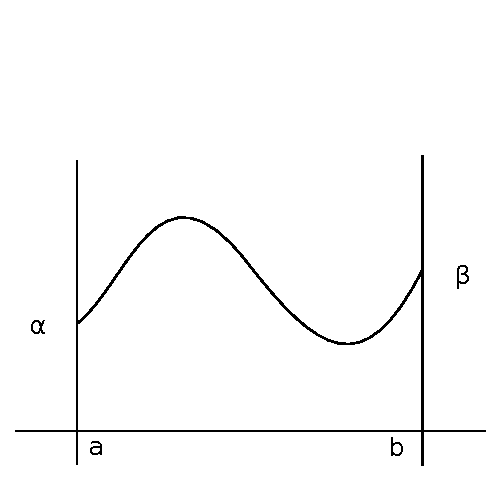
\includegraphics[width=0.3\textwidth]{img/variation.pdf}
    \caption{Setting for examples in Variation Calculus}
    \label{img:var}
  \end{center}
\end{figure}

\begin{ex}
  Find $y \in \mathcal H = \set{y \in \mathcal C^2[a,b]: y(a) = \alpha, y(b) = \beta}$ such that $F(x) \coloneqq \pi \int_a^b y(x) \sqrt{1 + (y'(x))^2} \, dx$
  which represents the surface of a rotational device with
  $F(x) \to \text{ min}$. Compare with Figure~\ref{img:rot}.
\end{ex}

\begin{figure}[!h]
  \begin{center}
    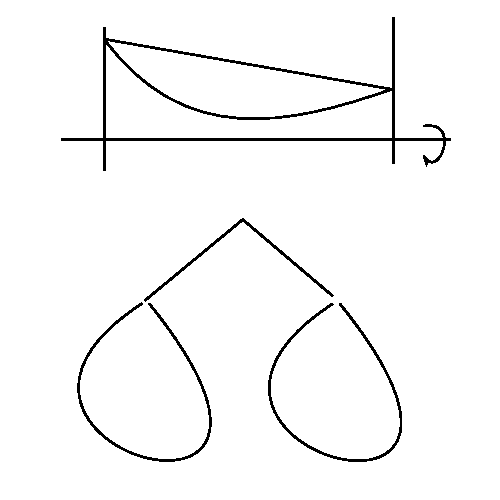
\includegraphics[width=0.3\textwidth]{img/var_problem_setting.pdf}
    \caption{Rotational device in our problem setting.}
    \label{img:rot}
  \end{center}
\end{figure}

Assume $y_{\text{min}}(x)$ is a solution to our problem.
For arbitrary $h$ such that $y_{\text{min}} + th \in H(\text{admissible set})$
it must holds that $F(y_{\text{min}} + th) \geq F(y_{\text{min}})$,
hence $f(t) = F(y_{\text{min}} + th)$ has a minimum in $t=0$ with $f'(0) = 0$.
\[ f(t) = \int_a^b L(x, y_{\text{min}}(x) + th(x), y'_{\text{min}}(x) + th'(x)) \, dx \to \text{min} \text{ at } t=0 \]

Necessary condition:
$f'(0) = 0$, derivative under integral
\[ \implies \int_a^b \left[\partial_y L(x, y_{\text{min}}(x), y_{\text{min}}'(x)) \cdot h(x) + \partial_p L(x, y_{\text{min}}(x), y_{\text{min}}'(x)) \cdot h'(x) \right] \, dx = 0 \]
$\forall h \in \mathcal C^2([a,b])$ with $h(a) = h(b) = 0$.

\[ \int_a^b \underbrace{\partial_p L(x, y_{\text{min}}(x), y_{\text{min}}'(x))}_{\coloneqq v} \cdot \underbrace{h'(x)}_{=u'} \, dx \]
We apply integration by parts:
\[ = \underbrace{h(x) \cdot \partial_p L(x, y_{\text{min}}(x), y_{\text{min}}'(x))}_{=0} \int_a^b - \int_a^b \partial_{xp} L(x, y_{\min}, y_{\min}') \]
\[ + \partial_{yp} L(x, y_{\min}, y_{\min}') \cdot y_{\min}' + \partial_{pp} L(x, y_{\min}, y_{\min}') \cdot y_{\min}'') \cdot h \, dx \]
So,
\[ \int_a^b \left[ \partial_y L(x, y, y') - \partial_{xp} L(x, y, y') - \partial_{yp} L(x, y, y') - \partial_{pp} L(x, y, y') \right] \cdot h \, dx = 0 \]
in $y = y_{\min}$. $\forall h \in \mathcal C^2([a,b])$ with $h(a) = h(b) = 0$.

\index[English]{Euler-Lagrange Equation}
\index[German]{\foreignlanguage{ngerman}{Euler-Lagrange Gleichung}}
It holds that
\[ Ly(x, y_{\min}, y_{\min}') - \partial_{xp} L(x, y_{\min}, y_{\min}') - \partial_{yp} L(x, y_{\min}, y_{\min}') y_{\min}' \]
\[ - \partial_{pp} L(x, y_{\min}, y_{\min}') y_{\min}'' = 0 \]
which is called \emph{Euler-Lagrange Equation} (EL).

Differential equation of second order for $y_{\min}$.
\[ y_{\min}(a) = \alpha \qquad y_{\min}(b) = \beta \]

\index[English]{Lagrange function}
\index[German]{\foreignlanguage{ngerman}{Lagrange Funktion}}
\index[English]{Variation}
\index[German]{\foreignlanguage{ngerman}{Variation}}
$L$ is called \emph{Lagrange function}.
$F(y_{\min} + th)$ is called \emph{variation of $y_{\min}$}.

Special case: $L = L(y, p)$, so it does not depend on $x$
(as for example in $L(y, p) = y \sqrt{1 + p^2}$).
Then it holds that
\[ L_y(y, y') - L_{yp}(y, y') \cdot y' - L_{pp}(y, y') \cdot y'' = 0 \]

\begin{lemma}
  If the Lagrange function does not depend on $x$,
  then for every solution $\varphi(x)$ of Euler-Lagrange
  equation, the expression
  \[ E_{\varphi}(x) = L_p(\varphi(x), \varphi'(x)) \cdot \varphi'(x) - L(\varphi(x), \varphi'(x)) \]
  is constant in regards of $x$.
\end{lemma}
\begin{proof}
  \[ E_{\varphi}'(x) = \text{(EL)} = 0 \]
  In our example,
  \[ L_p(y, p) = y \cdot \frac12 \cdot \frac{1}{\sqrt{1 + p^2}} \cdot 2p = \frac{yp}{\sqrt{1 + p^2}} \]
  \[ E_y = c \implies \frac{y y'}{\sqrt{1 + y'^2}} y' - y \sqrt{1 + y'^2} = c \]

  At the beginning of the derivation:
  \[ \partial_x [\partial_p L(y, y')] - \partial_y L(y, y') = 0 \]
  \[ \frac{d}{dx} \left[\frac{yy'}{\sqrt{1 + y'^2}}\right] - \sqrt{1 + y'^2} = 0 \]
  \[ \implies \frac{y}{\sqrt{1 + y'^2}} = \text{constant } c \]

  \[ y(x) = c \cosh{\frac{1}{c}(x - x_0)} \]
\end{proof}


%\index[English]{}
%\index[German]{\foreignlanguage{ngerman}{}}

\clearpage
\begin{otherlanguage}{ngerman}
\printindex[German]
\end{otherlanguage}
\printindex[English]

\end{document}

%%% Local Variables:
%%% mode: latex
%%% TeX-master: t
%%% End:
